\documentclass[a4paper,12pt,oneside]{book}
\usepackage[utf8]{inputenc}
\usepackage[USenglish]{babel}
\usepackage{amsmath}
%\usepackage[abbr]{harvard}
\usepackage{tabularx}
\usepackage{graphicx}
\usepackage{longtable}
\usepackage{fancyhdr}
\usepackage[hang,small,it]{caption}
\usepackage{mathdesign}
\usepackage{ctable}
\usepackage{rotating}
\usepackage{booktabs}

%\ShowDisplacementBoxes

%=======================================================================
% GENERAL SETTINGS
%=======================================================================
\oddsidemargin 40pt
\evensidemargin 40pt
\setlength{\captionmargin}{10pt}
\setlength{\parskip}{0.5em}
\setlength{\parindent}{0em}
\providecommand{\degrees}{{\char'027}}
\newcommand{\FigDir}{D:/UserData/sources/WOFOST/doc/figs}

%=======================================================================
% A BIT MORE COMPACT ITEM LIST
%=======================================================================
\newenvironment{itemize*}%
{\begin{itemize}%
        \setlength{\parskip}{0pt}%
        \setlength{\itemsep}{0pt}%
        \setlength{\parsep}{0pt}}%
    {\end{itemize}}

%more compact enumeration list
\newenvironment{enumerate*}%
{\begin{enumerate}%
        \setlength{\itemsep}{0pt}%
        \setlength{\parskip}{0pt}}%
    {\end{enumerate}}

%=======================================================================
% A BIT MORE COMPACT DESCRIPTION LIST
%=======================================================================
\renewcommand{\descriptionlabel}[1]{\hspace{\labelsep}\textrm{#1}}

\newenvironment{description*}%
{\begin{description}%
        \setlength{\itemsep}{0pt}%
        \setlength{\parskip}{0pt}}%
    {\end{description}}

%=======================================================================
% DEFINITION OF THE FANCY HEADERS
%=======================================================================
\pagestyle{fancy}
\renewcommand{\chaptermark}[1]{\markboth{#1}{}}
\renewcommand{\sectionmark}[1]{\markright{\thesection\ #1}}
\fancyhf{}
\fancyhead[LE,RO]{\bfseries\thepage}
\fancyhead[LO]{\bfseries\rightmark}
\fancyhead[RE]{\bfseries\leftmark}
\headheight 15pt

\fancypagestyle{plain}{%
    \fancyhead{} % get rid of headers
    \renewcommand{\headrulewidth}{0pt} % and the line
}
\renewcommand{\headrulewidth}{0.4pt}

%=======================================================================
% MIXED EQUATION NUMBERS
% This is to allow mixed equation number, see also:
% http://tex.stackexchange.com/questions/34566/mixed-subequation-numbering-within-an-array#34568
%=======================================================================
\usepackage{etoolbox}% http://ctan.org/pkg/etoolbox
\AtBeginEnvironment{align}{\setcounter{subeqn}{0}}% Reset subequation number at start of align
\newcounter{subeqn} \renewcommand{\thesubeqn}{\theequation\alph{subeqn}}%
\newcommand{\subeqn}{%
  \refstepcounter{subeqn}% Step subequation number
  \tag{\thesubeqn}% Label equation
}  

% PDF formatting
\usepackage[pdftitle={System description of the WOFOST 6.0 crop simulation model Implemented in CGMS},pdfpagemode=UseOutlines, pdfauthor={Allard de Wit}, pdfpagetransition=Dissolve, bookmarks=true]{hyperref}


\begin{document}

\frontmatter
\tableofcontents
\listoffigures
\listoftables
\cleardoublepage

\mainmatter

\chapter{Introduction} 

\section{About WOFOST}

WOFOST is the acronym for WOrld FOod STudies. It is the name of a model for
simulating the growth of crops. WOFOST has been continuously developed by
Wageningen Research and Wageningen University (and its predecessors) already
since the 1980-ies. The current version 8.0 is maintained by Wageningen 
Research and several implementation of the model are available which have been
developed for both research and operational applications.

for a generic introduction and overview to the WOFOST model see:
Wit, Allard de, Hendrik Boogaard, Davide Fumagalli, Sander Janssen, Rob Knapen, 
Daniel van Kraalingen, Iwan Supit, Raymond van der Wijngaart, and Kees van Diepen. 
“25 Years of the WOFOST Cropping Systems Model.” Agricultural Systems 168 
(January 1, 2019): 154–67. https://doi.org/10.1016/j.agsy.2018.06.018.

\section{Levels of crop production}
Three levels of plant
production are distinguished. The crop production systems at any of these levels can
be considered as members of a broad class. In order of decreasing yield, these levels
are (Penning de Vries et al. 1989):

{\it Potential yield level\/}\\
This is the potential production situation. The crop has ample water and nutrients.
Crop yield depends on the initial conditions, weather (temperature and radiation)
and crop features (mainly growing season length).
Dry matter production, in case of full canopy, amounts 150-350 kg ha$^{{\rm -1}}$d$^{{\rm -1}}$. This
production level will be reached in laboratory experiments, glasshouses and with
intensive farming systems.

{\it Attainable yield level\/}\\
In this scenario the yield of the crop is limited by the availability of water and/or nutrients 
during a part or the complete
growing season. In such a scenario the yield will be reduced but still crop management is assumed to be 
optimal.

{\it actual yield level\/}\\
In this scenario the crop yield can be further reduced by factors such as pest, disease, competition with weeds
or polutants such as ozone, salt or heavy metals. This yield level reflects what farmers actual
harvest from their fields. The gap between the different yield levels (yield gap) varies widely
across the globe and finding approaches to close the yield gap is a an area of intense research,
see http://yieldgap.org

Note that the WOFOST crop simulation models can be applied in the domain of potential crop
production and production with a water shortage and/or nutrient shortage.
(Potential and attainable yield levels). 


\section{Guide to this manual}

This manual covers a detailed description of the processes of crop growth and water movement as they are
implemented in WOFOST Version 8.0. First of all, ancillary calculation will be described including:
\begin{itemize}
	\item derived meteorological variables
	\item reference evapotranspiration
	\item day length and solar elevation
	\item extra terrestrial radiation
\end{itemize}

Next, the different components of the crop simulation itself will be described in detail:
\begin{itemize}
	\item phenology
	\item transpiration
	\item assimilation:
	\subitem gross photosynthesis rate
	\subitem Correction for temperature
	\subitem Correction for water/nutrient stress
	\item Maintenance respiration
	\item growth of the crop:
	\subitem Net photosynthesis rate
	\subitem growth respiration
	\subitem partitioning
	\subitem leaf growth and senescence 
	\subitem stems
	\subitem Roots
	\subitem storage organs	
	\item nutrients in the crop
\end{itemize}

Finally, the soil components are described which consist of several water balance implementations and the components for soil nutrients:
\begin{itemize}
	\item the 'classic' dual layer (rooted, unrooted) soil water balance 
	\item the multi-layer soil water balance including ground water influence
	\item the soil nutrient balance
\end{itemize}

\chapter{Ancillary calculations}


\section{Preparatory (weather) variables}


The average temperature is calculated as the average of the minimum and the maximum
temperature. This average temperature \={T} is equal to the so called air temperature (T) used
in the model calculations. The maximum and minimum temperature are measured daily values or
derived from other sources such as a weather forecasting model.

\begin{equation}
T ~=~{\frac{T _{\max } ~+~ T _{\min } }{2}}
\end{equation}

Where:\\[5pt]
\begin{tabularx}{\textwidth}{llXr}
	T &:& Average daily air temperature & [\degrees C]\\
	T$_{{\rm max}}$&:  & Maximum temperature & [\degrees C]\\
	T$_{{\rm min}}$&: &  Minimum temperature & [\degrees C]\\
\end{tabularx}

Similarly, the daytime average temperature can be estimated as: 

\begin{equation}
% eq 5.32
\label{eq:daytimetemp}
T_{day} = {\frac{T_{\max} + T}{2}} ~~~~ where ~~~~ T = {\frac{T_{\max } + T_{\min}}{2}}
\end{equation}



The difference between maximum and minimum temperature is used to calculate the
empiric constant of the wind function in the Penman equation.

\begin{equation}
\Delta T ~= ~T _{\max } ~-~ T _{\min } 
\end{equation}

Where:\\[5pt]
\begin{tabularx}{\textwidth}{llXr}
	$\Delta$T& :& Temperature difference  &[\degrees C]\\
	T$_{{\rm max}}$ &:& Maximum temperature &  [\degrees C]\\
	T$_{{\rm min}}$& :& Minimum temperature  &[\degrees C]
\end{tabularx}


As will be explained later in \S \ref{sec:penman}, the evaporative demand, EA, depends on the 
windspeed and the difference between saturated and actual vapor pressure. The windspeed
dependency is incorporated in the evaporative demand as the windspeed measured at a
height of two meters, and multiplied by an empirical coefficient (see also eq. 
\ref{eq:EvapDemand}). This
coefficient is temperature dependent and can be calculated as (Fr\`{e}re, 1979):

\begin{align}
\label{eq:BU}
BU &= 0.54 ~+ ~0.35\,{\frac{\Delta T\, - 12}{4}} & for~~~\Delta ~ T~\ge ~ 12 \degrees C \\[1em]
\nonumber
BU &= 0.54 & for~~~\Delta ~ T~<~12 \degrees C
\end{align}

Where:\\[5pt]
\begin{tabularx}{\textwidth}{llXr}
	BU & :& Empirical coefficient in the wind function &  [-]\\
	$\Delta$T& :& Temperature difference & [\degrees C] \\
\end{tabularx}
\hspace*{6em}

The air temperature can be used to calculate the latent heat of vaporization: 

\begin{equation}
{\it \lambda} ~=~ 2.501~ -~ (2.361 \cdot 10^{-3} )\, T
\end{equation}

Where:\\[5pt]
\begin{tabularx}{\textwidth}{llXr}
	$\lambda$& :& Latent heat of vaporization & [MJ kg$^{{\rm -1}}$]\\
	T &:& Average daily temperature & [\degrees C]\\
\end{tabularx}


As the value of the latent heat varies only slightly over normal temperature ranges a
single value for $\lambda$ may be taken. In the model for $\lambda$ a value of 2.45 MJ 
kg$^{{\rm -1}}$ is assumed (T=20\degrees C). The barometric pressure at sea level is 
used to calculate the psychrometric constant at sea level (Brunt, 1932).

\begin{equation}
\gamma _{o} ~=~ {{\frac{\it C _{p} \, P _{o} }{{\it  \epsilon \, \lambda } }} }\, 10 ^{-3} ~=~ 0.00163\,{\it P} _{\frac{o}{\it \lambda}} 
\end{equation}

Where:\\[5pt]
\begin{tabularx}{\textwidth}{llXr}
	$\gamma$$_{{\rm o}}$ & :& Psychrometric constant at sea level & [kPa 
	\degrees C$^{{\rm -1}}$]\\
	C$_{{\rm p}}$ & :& Specific heat of moist air = 1.013 10$^{{\rm -3}}$ & [MJ kg$^{{\rm -1}}$ 
	\degrees C$^{{\rm -1}}$]\\
	P$_{{\rm o}}$ & :& Atmospheric pressure at sea level & [kPa]\\
	$\epsilon$ & :& Ratio molecule weight water vapor / dry air = 0.622 & []\\
	$\lambda$ & :& Latent Heat of vaporization & [MJ kg$^{{\rm -1}}$]\\
\end{tabularx}


In the model however, a fixed value of $\gamma$$_{{\rm o}}$ = 0.67 is assumed. This 
value can be obtained by using for P the atmospheric pressure at sea level, which is 
assumed to be 101.3 kPa and $\lambda$ = 2.45 MJ kg$^{{\rm -1}}$. It should be mentioned, 
that the barometric pressure changes with altitude, so does also the psychrometer constant. 
Therefore, the two following equations are used to correct for altitude difference.

\begin{equation}
P~=~P _{o} \, e ^{{\frac{-0.034\, z}{T\, +\, 273}} }
\end{equation}

Where:\\[5pt]
\begin{tabularx}{\textwidth}{llXr}
	P &:& Atmospheric pressure at elevation z  & [kPa]\\
	P$_{{\rm o}}$ &:& Atmospheric pressure at sea level  & [kPa]\\
	T &:& Daily temperature  & [\degrees C]\\
	z &:& Elevation  & [m]
\end{tabularx}

\begin{equation}
\label{eq:Psycho}
\gamma ~=~ \gamma _{o} \,{\frac{P}{P _{o} }}
\end{equation}

Where:\\[5pt]
\begin{tabularx}{\textwidth}{llXr}
	$\gamma$ &:& Psychrometric constant at elevation z & [kPa \degrees C]\\
	$\gamma$$_{{\rm o}}$ &:& Psychrometric constant at sea level & [kPa \degrees C]\\
	P &:& Atmospheric pressure at elevation z & [kPa]\\
	P$_{{\rm o}}$ &:& Atmospheric pressure at sea level & [kPa]\\
\end{tabularx}

The saturated vapor pressure is related to the mean daily air temperature and may be
approxi\-mated with the equation of Goudriaan (1977). 

\begin{equation}
\label{eq:SVP}
e_{s} ~=~ 0.610588\, \cdot \, e ^{{\frac{17.32491\, T}{T\, +\, 238.102}} }
\end{equation}

Where:\\[5pt]
\begin{tabularx}{\textwidth}{llXr}
	e$_{{\rm s}}$ &:& Saturated vapor pressure  & [kPa]\\
	T &:& Air temperature & [\degrees C]
\end{tabularx}

From this equation the derivate, i.e. the slope of the saturated vapor pressure-temperature
curve is established.

\begin{equation}
\label{eq:SlopeSVP}
\Delta ~=~{\frac{238.102 \cdot 17.32491 \cdot e_{s} }{(T + 238.102)^{2} }}
\end{equation}

Where:\\[5pt]
\begin{tabularx}{\textwidth}{llXr}
	$\Delta$ &:& Slope of the saturation vapor pressure curve  & [kPa \degrees C$^{{\rm -1}}$]\\
	e$_{{\rm s}}$ &:& Saturated vapor pressure &  [kPa]\\
	T &:& Air temperature & [\degrees C]
\end{tabularx}

The measured vapor pressure is not allowed to exceed the calculated saturated vapor
pressure.

\section{Methods to estimate global radiation}

In case no observations for the incoming solar radiation are available, the formula
postulated by \AA ngstr\"{o}m (1924) can be used to estimate this parameter using sunshine
duration observations.

\begin{equation}
\label{eq:GlobRad}
S _{g,d} ~=~S _{o,d} \, (A\, +\, B\,{\frac{n}{D}} )
\end{equation}

Where:\\[5pt]
\begin{tabularx}{\textwidth}{llXr}
	S$_{{\rm g,d}}$ &:& Incoming daily global solar radiation  & [J m$^{{\rm -2}}$ d$^{{\rm -1}}$]\\
	S$_{{\rm o,d}}$ &:& Daily extra-terrestrial radiation (see eq. \ref{eq:Angot}) 
	& [J m$^{{\rm -2}}$ d$^{{\rm -1}}$]\\
	A &:& Empirical constant  & [-]\\
	B &:& Empirical constant  & [-]\\
	n &:& Bright sunshine hours per day  & [hr]\\
	D &:& Astronomical day length (see e.q. \ref{eq:irrad_diffuse})  & [hr]
\end{tabularx}

It should be mentioned that the empirical constants A and B of the \AA ngstr\"{o}m formula 
can be found with linear regression by comparing the incoming global radiation with the
relative sunshine duration n/D, taking into consideration the daily extra-terrestrial
radiation. A is the intercept and B the slope of the regression. It should also be mentioned
that the regression constants A and B have a physical meaning. A can be considered as
the fraction of extra terrestrial radiation on overcast days. The sum of A and B can be
considered as the fraction of radiation received on clear days.
For several regions in Europe the \AA ngstr\"{o}m constants have been established by Supit
(1994). Indicative values for empirical constants in the \AA ngstr\"{o}m formula are 
depicted in Table \ref{tab:angstAB}.

\begin{table}
	\centering
	\caption{Indicative values for empirical constants in the \AA ngstr\"{o}m formula in
		relation to latitude and climate used by the FAO (Fr\`{e}re \& Popov, 1979)}
	\label{tab:angstAB}
	\begin{tabular}{lcc}
		\hline
		Zone &   A &  B  \\
		\hline
		Cold and temperate zones   &  0.18 &  0.55\\
		Dry tropical zones  &   0.25  & 0.45\\
		Humid tropical zones  &   0.29 &  0.42\\
		\hline
	\end{tabular}
\end{table}

It should be clear that the constants {\bf A} and {\bf B} (acronym: {\bf COEFA} and {\bf COEFB}) should be
provided by the user. However, in case these constants are not available, in the JRC
version of WOFOST 6.0 (in subroutine {\bf METEO}), the following approximation is used:

\begin{align*}
A &=~0.4885~-~0.0052 \, LAT \\
B &=~0.1563~+~0.0074 \, LAT 
\end{align*}

Where:\\[5pt]
\begin{tabularx}{\textwidth}{llXr}
	A &:& Empirical constant  & [-]\\
	B &:& Empirical constant  & [-]\\
	LAT &:& Latitude  & [degrees]\\
\end{tabularx}

As an improvement, in future versions of WOFOST, the method developed by Supit
(1994) will be introduced in the model. This method calculates the incoming global
radiation as a function of cloud cover and sunshine duration. It can be considered as an
extension of the formula developed by Hargreaves (1985). 
Using this method, the accuracy of the results is slightly less in comparison to 
the results obtained with the \AA ngstr\"{o}m formula.

\begin{equation}
S _{g,d} ~=~ c _{a} \, S _{o,d} \, (\sqrt{(T _{\max} ~-~T _{\min} )} ~+~ 
c _{b} \sqrt{(1-{Cloud/8})} ~) ~+~c _{c} 
\end{equation}

Where:\\[5pt]
\begin{tabularx}{\textwidth}{llXr}
	S$_{{\rm g,d}}$ &:& Incoming daily global solar radiation  & [J m$^{{\rm -2}}$ d$^{{\rm -1}}$]\\
	S$_{{\rm o,d}}$ &:& Daily extra-terrestrial radiation (see eq. \ref{eq:Angot})  & 
	[J m$^{{\rm -2}}$ d$^{{\rm -1}}$]\\
	Cloud &:& Mean total cloud cover during daytime  & [octas]\\
	T$_{{\rm max}}$ &:& Maximum temperature  & [\degrees C]\\
	T$_{{\rm min}}$ &:& Minimum temperature  & [\degrees C]\\
	c$_{{\rm a}}$,c$_{{\rm b}}$,c$_{{\rm c}}$ &:& Empirical regression constants   & [-]
\end{tabularx}

For five regions in Europe the constants c$_{{\rm a}}$, c$_{{\rm b}}$ and c$_{{\rm c}}$ 
have been established (Supit, 1994).

As a second improvement, the Hargreaves formula (1985) will be introduced in the
model. In case no observations of either incoming radiation, sunshine duration and
cloudcover are available, this formula, will be used. The accuracy of this method is less
then the accuracy of the two earlier mentioned methods.

\begin{equation}
S _{g,d} ~=~ c _{d} \, S _{o,d} \, \sqrt{(T _{\max} ~-~T _{\min} )} ~+~c _{e} 
\end{equation}

Where:\\[5pt]
\begin{tabularx}{\textwidth}{llXr}
	S$_{{\rm g,d}}$ &:& Incoming daily global solar radiation  & [J m$^{{\rm -2}}$ d$^{{\rm -1}}$]\\
	S$_{{\rm o,d}}$ &:& Daily extra-terrestrial radiation (see eq. \ref{eq:Angot})  & 
	[J m$^{{\rm -2}}$ d$^{{\rm -1}}$]\\
	T$_{{\rm max}}$ &:& Maximum temperature  & [\degrees C]\\
	T$_{{\rm min}}$ &:& Minimum temperature  & [\degrees C]\\
	c$_{{\rm d}}$,c$_{{\rm e}}$  &:& Empirical regression constants  & [-]\\
\end{tabularx}

For six regions in Europe the constants c$_{{\rm d}}$ and c$_{{\rm e}}$ have been 
established (Supit, 1994). In section \ref{sec:daylength} it is explained how the 
daily extra-terrestrial radiation, S$_{{\rm o,d}}$, can be calculat\-ed.

\section{Reference evapotranspiration}

Strictly speaking, transpiration is the loss of water from the plants, and evaporation is the
loss of water from the soil or from a free-water surface. Evapotranspiration covers both
transpiration and evaporation.
The principal driving force for evaporation is the gradient of vapour pressure between the
evaporating surface and the surrounding air. The vapour pressure at the evaporating
surface is equal to the saturated vapour pressure at the prevailing temperature of that
surface. The vapour pressure of the air is a function of the ambient temperature and its
relative humidity. The rate of evaporation depends on the diffusion resistance between the
evaporating surface and the air.
The magnitude of the resistance is strongly related to wind speed. The two environ\-mental
variables, air humidity and wind speed combined determine the 'evaporative demand' of
the air.

The problem in the approach above is that the temperature of the evaporating surface is
usually not known from standard meteorological observations. Evaporation  of 1 mm
layer of water requires 2.45 MJ m$^{{\rm -2}}$ of energy and can therefore be described through
quantification of an energy balance. The energy dissipation, required for evaporation,
leads to cooling of the evaporating surface which reduces the vapour gradient. Hence, a
driving force is required to maintain the corresponding surface temperature, and thus,
maintain the vapour pres\-sure gradient. The energy for this driving force is supplied by the
net solar radiation received by the canopy and or soil.
Net radiation is the balance between incoming (short-wave) radiation from the sun and
radiation losses due to reflection and outgoing (long-wave) radiation. Heat supplied by
moving air is another source of energy, but this is usually negligible, except in situations
where the vegetation is surrounded by extensive bare areas (oasis). Only 5-8\% of
incoming radiation is dissipated in photosynthesis, which is, therefore, disregarded here.
Respiration yields an insignificant amount of energy. To simplify the treatment of
evapotranspiration, it is considered to be governed by two factors: radiation and evaporative demand.

Penman (1948) was the first to describe evapotranspiration in physical mathematical
terms. He calculated evaporation from free-water surfaces, wet bare soil and low grass
swards for 10-day periods. The original Penman reference evapotranspiration has now been 
superseded by the 
Penman-Monteith reference evapotranspiration. The latter has a better physical basis and
is standardized and promoted by the Food and Agriculture Organization. WOFOST uses the
Penman-Monteith equation to compute the crop reference evapotranspiration but still applies
the older Penman approach as reference evapotranspiration for open water and bare soil.
Moreover, the option to use the older Penman approach as reference evapotranspiration is still
available in order to compare with historical studies.

The value calculated according to the P/PM equations is the potential evapotranspiration, 
i.e. without limitations with respect to the supply of liquid water to the
evaporating surface. This ET0 value is often used as a reference value, to
which actual crop water demand is related. To translate ET0 into crop water require\-ments,
so called crop factors can be used (e.g. Doorenbos \& Pruitt, 1977; Feddes {\it et al.},
1978). See also \S \ref{sec:evapotranspiration}.

Note that the equations used to compute ET0 provide the value in mm/day while internally
this is converted into cm/day.

\subsection{Terms in the Penman formula}
\label{sec:penman}

The Penman formula (equation \ref{eq:ET0}) consists of two segments. The first part, the radiative
term, calculates the net absorbed radiation. The second part, the aerodynamic term,
calculates the evapora\-tive demand of the atmo\-sphere (Choisnel {\it et al}., 1992; Fr\`{e}re and
Popov, 1979; Penman, 1956, 1948). The resulting equations are used to calculate the
potential evapora\-tion rates from a water surface, from bare soil surfaces and the potential
evapotranspira\-tion rate from a crop canopy.

\begin{equation}
\label{eq:ET0}
ET0 ~=~ W ~R _{na} ~+~(1\, -\, W) ~E _{a} 
\end{equation}

Where:\\[5pt]
\begin{tabularx}{\textwidth}{llXr}
	ET0&:& Evapo(transpi)ration & [mm d$^{{\rm -1}}$] \\
	W&:& Temperature related weighing factor &  [-] \\
	R$_{{\rm na}}$&: & Net absorbed radiation in equivalent evaporation & [mm d$^{{\rm -1}}$] \\
	EA&: &  Evaporative demand in equivalent evaporation & [mm d$^{{\rm -1}}$] \\
\end{tabularx}

The temperature related weighing factor W in equation \ref{eq:ET0} is defined as 
(Fr\`{e}re and Popov, 1979; Penman, 1948, 1956).

\begin{equation}
W ~=~{\frac{\Delta}{(\Delta ~+~ \gamma )}} 
\end{equation}

Where:\\[5pt]
\begin{tabularx}{\textwidth}{llXr}
	$\Delta$ &:& Slope of the saturation vapor pressure curve (see eq. \ref{eq:SlopeSVP})  & [kPa \degrees C$^{{\rm -1}}$]\\
	$\gamma$ &:& Psychrometric constant (see eq. \ref{eq:Psycho})  & [kPa \degrees C$^{{\rm -1}}$]
\end{tabularx}

To calculate net outgoing long wave radiation Penman (1956) used an equation which is
derived from the formula postulated by Brunt (1932). The net outgoing long wave
radiation increases with increasing values for the mean air temperature and the relative
sunshine duration and decreases with increasing vapor pressure.

\begin{equation}
R _{nl} \uparrow  ~=~ \sigma \,\, (T+273) ^{4} \,\, (0.56\,\, -\,\, 0.079\, \sqrt{e _{a} } )\,\, (0.1\,\, +\,\, 0.9\,\,{\frac{n}{D}} )
\end{equation}


Where:\\[5pt]
\begin{tabularx}{\textwidth}{llXr}
	R$_{{\rm nl}}$$\uparrow$ &:& Net outgoing long-wave radiation & [J m$^{{\rm -2}}$ d$^{{\rm -1}}$]\\
	$\sigma$ &:& Stefan Boltzm\-ann constant = 4.90 x 10$^{{\rm -9}}$ & [J m$^{{\rm -2}}$ K$^{{\rm -4}}$ s$^{{\rm -1}}$]\\
	T &:& Air temperature & [\degrees C]\\
	e$_{{\rm a}}$ &:& Actual vapor pressure & [kPa]\\
	n/D &:& Relative sunshine duration & [-]\\
\end{tabularx}

The relative sunshine duration, n/D, is established in the model using:

\begin{equation}
{\frac{n}{D}} ~=~{\frac{T_{atm} ~-~A}{B}}
\end{equation}

Where:\\[5pt]
\begin{tabularx}{\textwidth}{llXr}
	n/D &:& Relative sunshine duration  & [-]\\
	T$_{{\rm atm}}$ &:& Atmospheric transmission (see eq. \ref{eq:Tatm})  & [-]\\
	A &:& Empirical constant in the \AA ngstr\"{o}m equation  & [-]\\
	B &:& Empirical constant in the \AA ngstr\"{o}m equation  & [-]\\
\end{tabularx}


The calculation of the atmospheric transmission, T$_{{\rm atm}}$, will be explained in 
\S \ref{sec:daylength}.

Part of the actual received radiation is reflected by the surface. The fraction reflected
(albedo) is different for a water surface, a soil surface and a crop canopy. The absorbed
fraction of radiation actually received minus the net outgoing radiation equals the net
absorbed radiation, which is divided by the latent heat of vaporization of water to express
the amount of radiation in depth of evaporative water layer (mm d$^{{\rm -1}}$).

\begin{equation}
\label{eq:AbsGlobRad}
R _{na} ~=~{\frac{(1\, -\, \alpha )\,\, R _{av} \, -\, R _{nl} \uparrow  }{\lambda}}
\end{equation}


Where:\\[5pt]
\begin{tabularx}{\textwidth}{llXr}
	R$_{{\rm na}}$ &:& Net absorbed radiation  & [mm d$^{{\rm -1}}$]\\
	$\alpha$ &:& Albedo or reflection coefficient of regarded surface  & [-]\\
	R$_{{\rm av}}$ &:& Average radiation  & [J m$^{{\rm -2}}$ d$^{{\rm -1}}$]\\
	R$_{{\rm nl}}$$\uparrow$ &:& Net outgoing long-wave radiation  & [J m$^{{\rm -2}}$ d$^{{\rm -1}}$]\\
	$\lambda$ &:& Latent heat  & [J kg$^{{\rm -1}}$]\\
\end{tabularx}


The soil's albedo depends on the surface color and on the moisture content. Albedo
values for dry soil vary from 0.14 (clay) to 0.37 (dune sand). Ten Berge (1986) described
the depen\-dence of the albedo value on soil moisture in relation to the average water
content of the top soil layer. See Table \ref{tab:AlbedoSoils}. 
In WOFOST 7.1 the following values for the albedo are assumed: for bare soil
0.15, for a canopy  0.25 and for a water surface a value of 0.05.

\begin{table}
	\centering
	\caption{Albedo values for wet and dry soils (ten Berge, 1986)}
	\label{tab:AlbedoSoils}
	\begin{tabular}{lcc}
		\hline
		soil type & wet & dry\\
		\hline
		Dune sand  &   0.24 &  0.37 \\
		Sandy loam &    0.10-0.19 &  0.17-0.23\\
		Clay loam &    0.10-0.14 &  0.20-0.23\\
		Clay &    0.08 &  0.14\\
		\hline
	\end{tabular}
\end{table}

The evaporative demand of the atmosphere depends on the difference between saturated
and actual vapor pressure and on the wind function. For crop canopies the evaporative
demand is somewhat higher than for soil or water surfaces due to a higher surface
roughness. This is reflected in a higher value for {\it factor} in the wind function.

\begin{equation}
\label{eq:EvapDemand}
EA~=~0.26\, (e _{s} \, -\, e _{a} )\,\, (factor\, +\, BU\, u(2))
\end{equation}

Where:\\[5pt]
\begin{tabularx}{\textwidth}{llXr}
	EA &:& Evaporative demand  & [mm d$^{{\rm -1}}$]\\
	e$_{{\rm s}}$ &:& Saturated vapor pressure (see eq. \ref{eq:SVP})  & [kPa]\\
	e$_{{\rm a}}$ &:& Actual vapor pressure  & [kPa]\\
	{\it factor} &:& Empirical constant  & [-]\\
	BU &:& Coefficient in wind function (see eq. \ref{eq:BU})  & [-]\\
	u(2) &:& Mean windspeed at 2 m height  & [m s$^{{\rm -1}}$]\\
\end{tabularx}

The following values for {\it factor} are assumed (Fr\`{e}re, 1979). For crop canopies {\it factor} =
1.0 and for a free water a surface {\it factor} = 0.5.

Substituting equations \ref{eq:EvapDemand} and \ref{eq:AbsGlobRad} in equation \ref{eq:ET0} yields

\begin{equation}
\label{eq:Penman}
ET0 ~=~{\frac{(\Delta R _{na~} +~\gamma EA)}{\Delta ~+~\gamma }}
\end{equation}

Where:\\[5pt]
\begin{tabularx}{\textwidth}{llXr}
	ET0 &:& Evapo(transpiration)  & [mm d$^{{\rm -1}}$]\\
	R$_{{\rm na}}$ &:& Net absorbed radiation  & [mm d$^{{\rm -1}}$]\\
	EA &:& Evaporative demand  & [mm d$^{{\rm -1}}$]\\
	$\Delta$ &:& Slope of the saturation vapor pressure curve   & [kPa \degrees C$^{{\rm -1}}$]\\
	$\gamma$ &:& Psychrometric constant  & [kPa \degrees C$^{{\rm -1}}$]
\end{tabularx}

With the equations \ref{eq:AbsGlobRad}, \ref{eq:EvapDemand}, \ref{eq:Penman} and the different values for factor and albedo, the evapo(transpi)ration from a wet bare soil surface E0$_{{\rm s}}$, a water surface, E0$_{{\rm w}}$, and a crop canopy, ET0, can be easily calculated.

Measured or estimated daily global irradiation (wavelength 300-3000 nm) is input in the
model (R$_{{\rm av}}$=S$_{{\rm g,d}}$ is assumed). It should be mentioned that the dimension of E0$_{{\rm s}}$, E0$_{{\rm w}}$ and ET0 is mm d$^{{\rm -1}}$ in subroutine {\bf PENMAN}. However, in all the other routines the dimension of these variables is cm d$^{{\rm -1}}$. In the routine {\bf METEO} the dimension of E0$_{{\rm s}}$, E0$_{{\rm w}}$ and ET0 is changed to cm d$^{{\rm -1}}$.


\subsection{Terms in the Penman-Monteith formula}

The Penman-Monteith equation implemented in WOFOST closely follows the algorithm laid down in 
FAO Irrigation and drainage paper 56 ("Crop evapotranspiration - Guidelines for computing crop 
water requirements") by Allen et al. (1998) which is available online \footnote{http://www.fao.org/3/X0490E/x0490e00.htm}
and will not be repeated here.

Standard values for the reference canopy reflection and canopy resistance of 0.23 and 70 $s m^{-1}$ are used and
the soil heat flux is explicitly set to zero. Moreover, some of the terms in the FAO PM equation have been
rearranged for clarity. For example the magic number "0.408" in the FAO equation can be more easily 
understood as one divided by the latent heat for vaporisation.


\section{Day length and solar elevation}
\label{sec:daylength}

Subroutine {\bf ASTRO} calculates day length, some intermediate variables for the calculation
of the solar elevation, the integral of the solar elevation over a day and the fraction of
diffuse radiation.

Day length is a function of the angle of the sun above the horizon (solar elevation). Solar
elevation is the angle between the sun rays and the earth's surface. Solar elevation is
determined by latitude, the day and the hour on a certain day.
The dependency on the hour of a certain day is simple to explain. The sun rises and the
sun sets every day. Just before sun rise and just after sun set the solar elevation is zero. 
At the equator on days that the sun is in zenith (the point in the sky directly overhead) at 
12 o'clock solar time it holds that:

\begin{equation}
\sin \beta = \cos (15(t _{h} -12))
\end{equation}

Where:\\[5pt]
\begin{tabularx}{\textwidth}{llXr}
	$\beta$ &:& Solar elevation  & [degrees]\\
	t$_{{\rm h}}$ &:& Hour of the day  & [h]\\
\end{tabularx}

The angle of the sun changes during the day because the earth rotates once around its axis
every 24 hours at a speed of 15\degrees per hour (= 360/24).  

To explain the dependency of solar elevation on latitude and day number first the situation
is regarded when the sun is in zenith. This is at 12 o'clock solar time (not to be mixed up
with noon). The solar declination, the place were the sun is in zenith at 12 o'clock solar
time, changes every day. On the 21$^{\rm st}$ of June the sun stands perpen\-dicular above 
the northern tropic of Cancer (+23.45\degrees N) and on the 22$^{\rm nd}$ of December the 
stands perpendicular above the tropic of Capricorn (-23.45\degrees S). In figure 
\ref{fig:solardecl} the situation is depicted for 22$^{\rm nd}$ of December when the sun 
reaches its highest point at the tropic of Capricorn at the southern hemisphere. On the 
northern hemisphere this results in the shortest day of the year.

\begin{figure}[p]
	\centering
	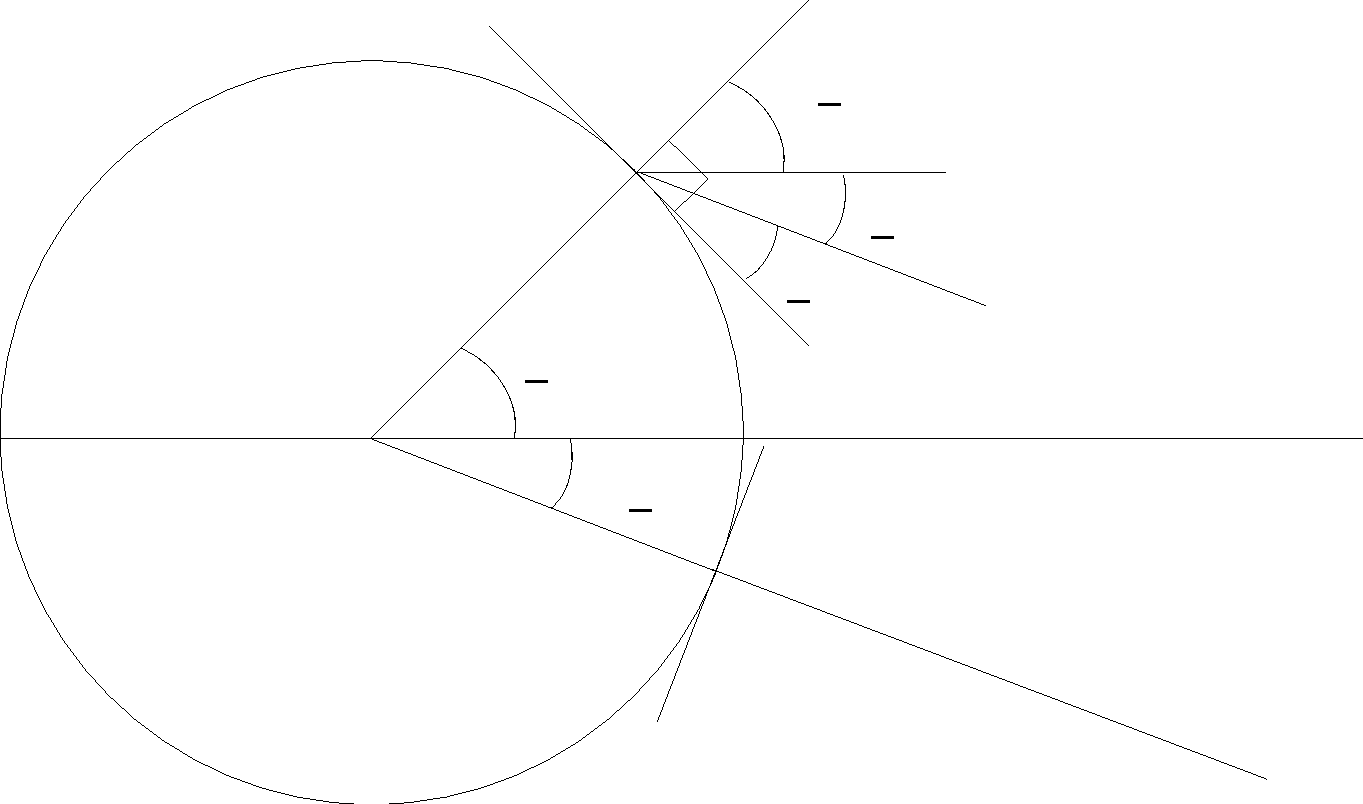
\includegraphics[width=93mm]{\FigDir/AARDE3.pdf}
	\caption{Solar declination}
	\label{fig:solardecl}
	%\begin{forcewidth}{9.33cm}
	% \begin{center}\InputPS{\FigDir/AARDE3.eps} \end{center}
	%\end{forcewidth}
\end{figure}

The solar declination during the year can be approached by a cosine function. (Note a shift of ten days).

\begin{equation}
\delta ~=~ -23.45 \cos ( 2 \pi {\frac{t _{d} + 10}{365}} )
\end{equation}

Where:\\[5pt]
\begin{tabularx}{\textwidth}{llXr}
	$\delta$ &:& Solar declination   & [de\-grees]\\
	t$_{{\rm d}}$ &:& Number of the day since 1 January   & [-]\\
\end{tabularx}

The distance of the sun to the earth is considered to be infinite, therefore declination 
can be considered equal for all places on earth. The orbit of the earth around the sun is a
non concentric ellipse (see figure \ref{fig:orbit}), therefore the solar radiation received 
at the top of the atmosphere during the year is not constant. At the first of January the 
earth is closest to the sun, radiation at the top of the atmosphere will then be higher as 
during other days.

\begin{figure}p]
	\centering
	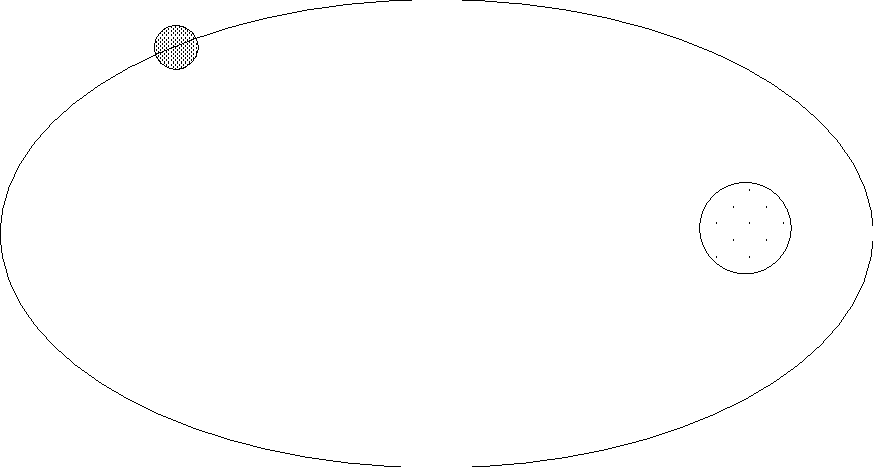
\includegraphics[width=80mm]{\FigDir/ELIPS.pdf}
	\caption{Orbit of the earth around the sun}
	\label{fig:orbit}
	%\begin{forcewidth}{7.77cm}
	%% \begin{center}\InputPS{\FigDir/ELIPS.eps} \end{center}
	%\end{forcewidth}
\end{figure}

The average solar radiation at the top of the atmosphere is estimated at 1370 W m$^{\rm -2}$. A daily solar radiation constant can than be calculated as a cosine times the average solar radiation at the top of the atmosphere multiplied by correction factor to correct for the elliptical orbit of the earth around the sun. This correction factor is estimated to be 0.033.

\begin{equation}
\label{eq:SolarConst}
S _{c,d} = S _{c} (1+0.033 \cos (2 \pi {\frac{t _{d} }{365}} ))
\end{equation}

Where:\\[5pt]
\begin{tabularx}{\textwidth}{llXr}
	S$_{{\rm c,d}}$ &:& Solar constant at the top of the atmosphere for a certain day  & [J m$^{{\rm -2}}$ s$^{{\rm -1}}$]\\
	S$_{{\rm c}}$ &:& Average solar radiation at the top of atmosphere (1370 J m$^{{\rm -2}}$ s$^{{\rm -1}}$; I.E.A., 1978) & [J m$^{{\rm -2}}$ s$^{{\rm -1}}$]\\
	t$_{{\rm d}}$ &:& Number of day since 1 January  & [-]\\
\end{tabularx}

Note that during the winter in Europe the solar radiation at the top of the atmo\-sphere is at 
its maximum! The height of the sun at any moment throughout the day and at any place and date can be
calculated with (subroutine {\bf ASTRO}):

\begin{equation}
\label{eq:SolarElevation}
\sin \beta = \sin \lambda \sin \delta + \cos \lambda \cos \delta \cos (2 \pi {\frac{(t _{h} +12)}{24}} )
\end{equation}

Where:\\[5pt]
\begin{tabularx}{\textwidth}{llXr}
	$\beta$ &:& Solar elevation  & [degrees]\\
	$\lambda$ &:& Latitude  & [degrees]\\
	$\delta$ &:& Solar declination  & [degrees]\\
	t$_{{\rm h}}$ &:& Hour of the day (solar time)  & [h]\\
\end{tabularx}

To compute day length for photoperiod-sensitive species, it must be realized that, even
when the sun is still below the horizon the light level is high enough to trigger the
photoperiodicity mechan\-ism. Photoperiodic day length is 0.5 h longer than the 
astronomi\-cal day length at the equator and about 0.8 h in temperate zones, depending 
on the date of the year. The light level to which photoperiodism is sensitive is quite low and not well
quantified. Vergara \& Chang (1985) determined it to be 1.5-15 mW m$^{{\rm -2}}$ for 
rice crops; Salisbury (1981) determined the level to be higher. As a compromise a value of 50 mW
m$^{{\rm -2}}$ is used in the model, which corresponds with a sun angle of -4 degrees. The
photosynthetic active period and the astro\-nomical day length can be calculated as:

\begin{equation}
% eq 4.25
\label{eq:AstroDaylength}
D ~=~ 12~+~{\frac{24}{180}} \, \arcsin \, (\,{\frac{-\sin {\frac{p}{180}} + sinLD}{cosLD}} )
\end{equation}

Where:\\[5pt]
\begin{tabularx}{\textwidth}{llXr}
	D &:& Day length  & [h]\\
	sinLD &:& Seasonal offset of sine of solar height = sin$\delta$sin$\lambda$  & [-]\\
	cosLD &:& Amplitude of sine of solar height = cos$\delta$cos$\lambda$  & [-]\\
	p &:& correction constant  & [degrees]\\
\end{tabularx}

The correction constant for the photosynthetic day length is -4 degrees. For the astronomical 
day length the correction constant is -0.833 degrees (i.e. solar height for which
the upper edge of the solar disk appears on the horizon). However, in the model for the
calculation of the astronomical day length, a correction constant of 0 degrees is used. 

The calculation of the photoperiodic day length makes no sense when the sun is continuously 
at higher inclinations, therefore this calculation method is limited to -66.5+4 and
66.5-4 degrees of latitude.

The integral of the solar height over the day can be obtained as twice the integral from
sunrise ($\beta$=0\degrees ) to 12 o'clock solar time ($\beta$ = 90\degrees  + $\delta$ - $\lambda$):

\begin{equation}
\label{eq:IntgrlSolarHeigh}
\int \sin \beta dt _{h} ~=~ 3600( D \sin \lambda \sin \delta +{\frac{24}{\pi }} \cos \lambda \cos \delta \sqrt{1-\tan^{2} \lambda \tan^{2} \delta } )
\end{equation}

Where:\\[5pt]
\begin{tabularx}{\textwidth}{llXr}
	$\int$sin$\beta$  &:& Integral solar height & [s]\\
	D  &:& Day length & [h]\\
	$\beta$  &:& Solar elevation & [degrees]\\
	t$_{{\rm h}}$  &:& Hour of the day & [h]\\
\end{tabularx}

Multiplication of equation \ref{eq:SolarConst} with \ref{eq:IntgrlSolarHeigh} yields the 
daily extra-terrestrial radiation which is also known as the Angot radiation. Note that 
the dimension of the daily extra-terrestrial is radiation J m$^{{\rm -2}}$ d$^{{\rm -1}}$.

\begin{equation}
% eq 4.27
\label{eq:Angot}
S_{o,d} = S _{c,d} ~ \int \sin \beta dt _{h} 
\end{equation}

Where:\\[5pt]
\begin{tabularx}{\textwidth}{llXr}
	S$_{{\rm o,d}}$ &:& Daily extra-terrestrial radiation  & [J m$^{{\rm -2}}$ d$^{{\rm -1}}$]\\
	S$_{{\rm c,d}}$ &:& Solar constant at the top of the atmosphere 
	for a certain day (see eq. \ref{eq:SolarConst}
	)  & [J m$^{{\rm -2}}$ s$^{{\rm -1}}$]\\
	t$_{{\rm d}}$ &:& Number of day since 1 January  & [-]\\
\end{tabularx}

In the model the integral of the effective solar height, a modification of equation \ref{eq:Angot} is
also calculated. This modified integral takes the effect of the daily course in atmospheric
transmis\-sion into account. Transmission is lower near the margins of the day because of
haze in the morning and clouds in the afternoon. Besides that, path length of solar
radiation in the atmosphere is longer (Spitters {\it et al}., 1986). This modified integral 
can be calculated as:

\begin{align}
% eq 4.28
\label{eq:IntSolarHeight}
\int \sin \beta_{m} &= \int \sin \beta (1+csin \beta ) dt_{h}  \\
&= 3600 \cdot \left \{
\begin{tabular}{c}
$D ( \sin \lambda \sin \delta + 0.4 
(( \sin \lambda \sin \delta )^{2} + 0.5( 
\cos \lambda \cos \delta ) ^{2} )) ~ + \nonumber$ \\[1em]
${\frac{12}{\pi}} \cos \lambda \cos 
\delta (2+3 \cdot 0.4 \sin \lambda \sin \delta ) 
\sqrt{1-\tan^{2} \lambda \tan^{2} \delta } \nonumber$
\end{tabular}
\right \}
\end{align}

Where:\\[5pt]
\begin{tabularx}{\textwidth}{llXr}
	$\int \sin \beta_{m}$  &:& Integral of effective solar height   & [s]\\
	D  &:& Day length       & [h]\\
	c  &:& Coefficient of regression on transmission on solar angle = 0.4  & [-]\\
	$\beta$  &:& Solar elevation   & [degrees]\\
	$\lambda$  &:& Latitude   & [degrees]\\
	$\delta$  &:& Solar declination   & [degrees]\\
	t$_{{\rm h}}$  &:& Hour of the day  f & [h]\\
\end{tabularx}

A distinction is made between diffuse sky light, with incidence under various angles and
direct sunlight with an angle of incidence equal to the solar declination. It is important 
to distin\-guish these fluxes because of the large difference in illumination intensity 
between shaded leaves and sunlit leaves and therefore the difference in the CO$_{{\rm 2}}$ 
assimila\-tion light response of single leaves, which is non-linear. Shaded leaves receive 
only diffuse radiation. Sunlit leaves receive both direct and diffuse radiation. The 
diffuse flux is the result of the scattering of sun rays by clouds, aerosols and gases in 
the atmo\-sphere. The propor\-tion of diffuse light in the total incident light flux depends 
on the status of the atmosphere, i.e. cloudi\-ness, concentra\-tion of aerosols. This 
fraction is calculated from the atmospheric transmis\-sion using an empirical function. 
This relationship is based on data from different meteorologi\-cal stations from a wide 
range of latitudes and longitudes (Spitters {\it et al}., 1986). 

The atmospheric transmission is the ratio between actual radiation and the quantity that
would have reached the earth's surface in the absence of an atmosphere (i.e. Angot
radiation). This ratio can be calculated as:

\begin{equation}
\label{eq:Tatm}
T _{atm} ~=~ s _{\frac{g,d}{S _{c,d} \int \sin \beta }}
\end{equation}

Where:\\[5pt]
\begin{tabularx}{\textwidth}{llXr}
	T$_{{\rm atm}}$ &:& Atmospheric transmission  & [-]\\
	S$_{{\rm g,d}}$ &:& Daily global radiation  & [J m$^{{\rm -2}}$ d$^{{\rm -1}}$]\\
	S$_{{\rm c,d}}$ &:& Solar constant at the top of the atmosphere for a certain day 
	(see eq. \ref{eq:SolarConst} and \ref{eq:Angot})  & [J m$^{{\rm -2}}$ s$^{{\rm -1}}$]\\
	$\int \sin \beta$  &:& Integral of solar height   & [s]\\
\end{tabularx}

Relationships between the share of the diffuse flux in the global irradiance 
(S$_{{\rm df}}$/S$_{{\rm g}}$) and the atmospheric transmission 
(S$_{{\rm g}}$/S$_{{\rm o}}$) are found in several research reports concerning the use
of solar energy in solar collectors. The relation is characterized by an approximately
linear trend for transmissions ranging between 0.35 and 0.75. At low transmissions,
nearly all of the incoming radiation is diffuse so that the curve bends off.
There is some variation among published relations, arising from differences in atmospheric 
conditions, especially relative sunshine duration, water content of the atmosphere,
and cloud type, but also lack of fit of the presented regression equation from the data and
differences in the method of measuring the diffuse radiation.

The relation used in WOFOST Version 6.0 has been derived by de Jong (1980) and has
been recommended by Spitters {\it et al}. (1986).

\begin{align}
% eq 4.30
\label{eq:irrad_diffuse}
{\frac{S _{df,d} }{S _{g, d} }} &= 1 & 
for ~~ {\frac{S _{g,d} }{S _{o,d} }} \le 0.07 \nonumber \\
{\frac{S _{df,d} }{S _{g,d} }} &= 1-2.3({\frac{S _{g,d} }{S _{o,d} }} -0.07) ^{2} & 
for ~~ 0.07 < {\frac{S _{g,d} }{S _{o,d} }} \le 0.35  \nonumber \\
{\frac{S _{df,d} }{S _{g,d} }} &= 1.33-1.46{\frac{S _{g,d} }{S _{o,d} }} &
for ~~ 0.35 < {\frac{S _{g,d} }{S _{o,d} }} \le 0.75 \nonumber \\
{\frac{S _{df,d} }{S _{g,d} }} &= 0.23 &
for ~~ {\frac{S _{g,d} }{S _{o,d} }} > 0.75 \nonumber \\
\end{align}

Where:\\[5pt]
\begin{tabularx}{\textwidth}{llXr}
	S$_{{\rm df,d}}$ &:& Daily diffuse radiation  & [J m$^{{\rm -2}}$ d$^{{\rm -1}}$]\\
	S$_{{\rm g,d}}$ &:& Daily global radiation  & [J m$^{{\rm -2}}$ d$^{{\rm -1}}$]\\
	S$_{{\rm o,d}}$ &:& Daily extra-terrestrial radiation (see eq. \ref{eq:Angot})  & 
	[J m$^{{\rm -2}}$ d$^{{\rm -1}}$]\\
\end{tabularx}

The relationships are remarkably constant over climates and latitudes so that the presented
equations will be valid for a wide range of conditions (Spitters {\it et al}., 1986).

Measured or estimated daily total solar irradiation (wavelength 300-3000 nm) is input for
the model. Only half of this incoming radiation is photosynthetical active (PAR,
Photosynthetically active radiation, wavelength 400 - 700 nm). The photosynthetically active
diffuse radiation, perpendicular to the direction of the solar rays can be calculated as:

\begin{equation}
% eq 4.31
\label{eq:PAR}
D _{p} ~=~ S _{\frac{df,d}{S _{g,d} }} ~~ T _{atm} ~0.5S _{c,d} 
\end{equation}


Where:\\[5pt]
\begin{tabularx}{\textwidth}{llXr}
	D$_{{\rm p}}$ &:& Diffuse irradiation perpendicular to the direction of light  & 
	[J m$^{{\rm -2}}$ s$^{{\rm -1}}$]\\
	T$_{{\rm atm}}$ &:& Atmospheric transmission (see eq. \ref{eq:Tatm})  & [-]\\
	S$_{{\rm c,d}}$ &:& Solar constant at the top of the atmosphere for a certain day  & 
	[J m$^{{\rm -2}}$ s$^{{\rm -1}}$]\\
	S$_{{\rm g,d}}$ &:& Daily global radiation  & [J m$^{{\rm -2}}$ d$^{{\rm -1}}$]\\
	S$_{{\rm df,d}}$ &:& Daily diffuse radiation (see eq. \ref{eq:irrad_diffuse})  & 
	[J m$^{{\rm -2}}$ d$^{{\rm -1}}$]\\
\end{tabularx}



\chapter{Crop development and growth}

\section{Overview of the crop growth model}

The WOFOST model describes phenological development, growth and yield formation of
a crop from emergence till maturity on the basis of crop genetic properties and 
environmental conditions. The model simulates dry matter accumulation of a crop as a function
of irradiation, temperature and crop characteristics in time steps of one day. 
The basis for calculating dry matter production, is the rate of gross CO$_{{\rm 2}}$ assimilation of
the canopy. This rate is dependent on the radiation energy absorbed by the canopy, which
is a function of incoming radiation and of crop leaf area. From the absorbed radiation and
the photosynthetic characteristics of single leaves, the daily rate of CO$_{{\rm 2}}$ assimilation of the
crop is calculated. Part of the carbohydrates produced (CH$_{{\rm 2}}$O) are used to provide energy
for the maintenance of the existing live biomass (maintenance respiration). The remaining
carbohydrates are converted into structural matter. In this conversion, some of the weight
is lost as growth respiration. The growth rate is thus obtained as:

\begin{equation}
% eq 5.1
\Delta W ~=~ C _{e} ~( A ~-~ R _{m} )
\end{equation}

Where:\\[5pt]
\begin{tabularx}{\textwidth}{llXr}
	$\Delta$W &:& Growth rate    &   
	[kg Dry Matter ha$^{{\rm -1}}$ d$^{{\rm -1}}$]\\
	A  &:& Gross assimilation   rate &  
	[kg CH$_{{\rm 2}}$O ha$^{{\rm -1}}$ d$^{{\rm -1}}$]\\
	R$_{{\rm m}}$  &:& Maintenance respiration rate    &  
	[kg CH$_{{\rm 2}}$O ha$^{{\rm -1}}$ d$^{{\rm -1}}$]\\
	C$_{{\rm e}}$ &:& Conversion efficiency off assimilates total crop   &   
	[kg Dry Matter kg$^{{\rm -1}}$ CH$_{{\rm 2}}$O]\\
\end{tabularx}

The dry matter produced is partitioned amongst the various plant organs such as roots,
leaves, stems and storage organs, using partitioning factors that are a function of the
phenological development stage of the crop (Spitters et al., 1989). The fraction partitioned
to the leaves, determines leaf area development and hence the dynamics of light interception. 
The dry weights of the plant organs are obtained by integrating their growth rates
over time (see eq. \ref{eq:euler_integration}).

Leaf mass is subdivided into age classes. During the development of the crop a part of
living biomass dies due to senescence. Some simulated crop growth processes are
influenced by temperature, like for example the maximum rate of photosynthesis and the
maintenance respiration. Other processes like the partitioning of assimilates or decay of
crop tissue are steered by the phenological stage. The phenological development stage is
calculated as a function of ambient temperature and possibly modified by the effect of day
length. An overview of all these processes is depicted in \ref{fig:CropGrowthProc2}.

\begin{figure}[p]
	\centering
	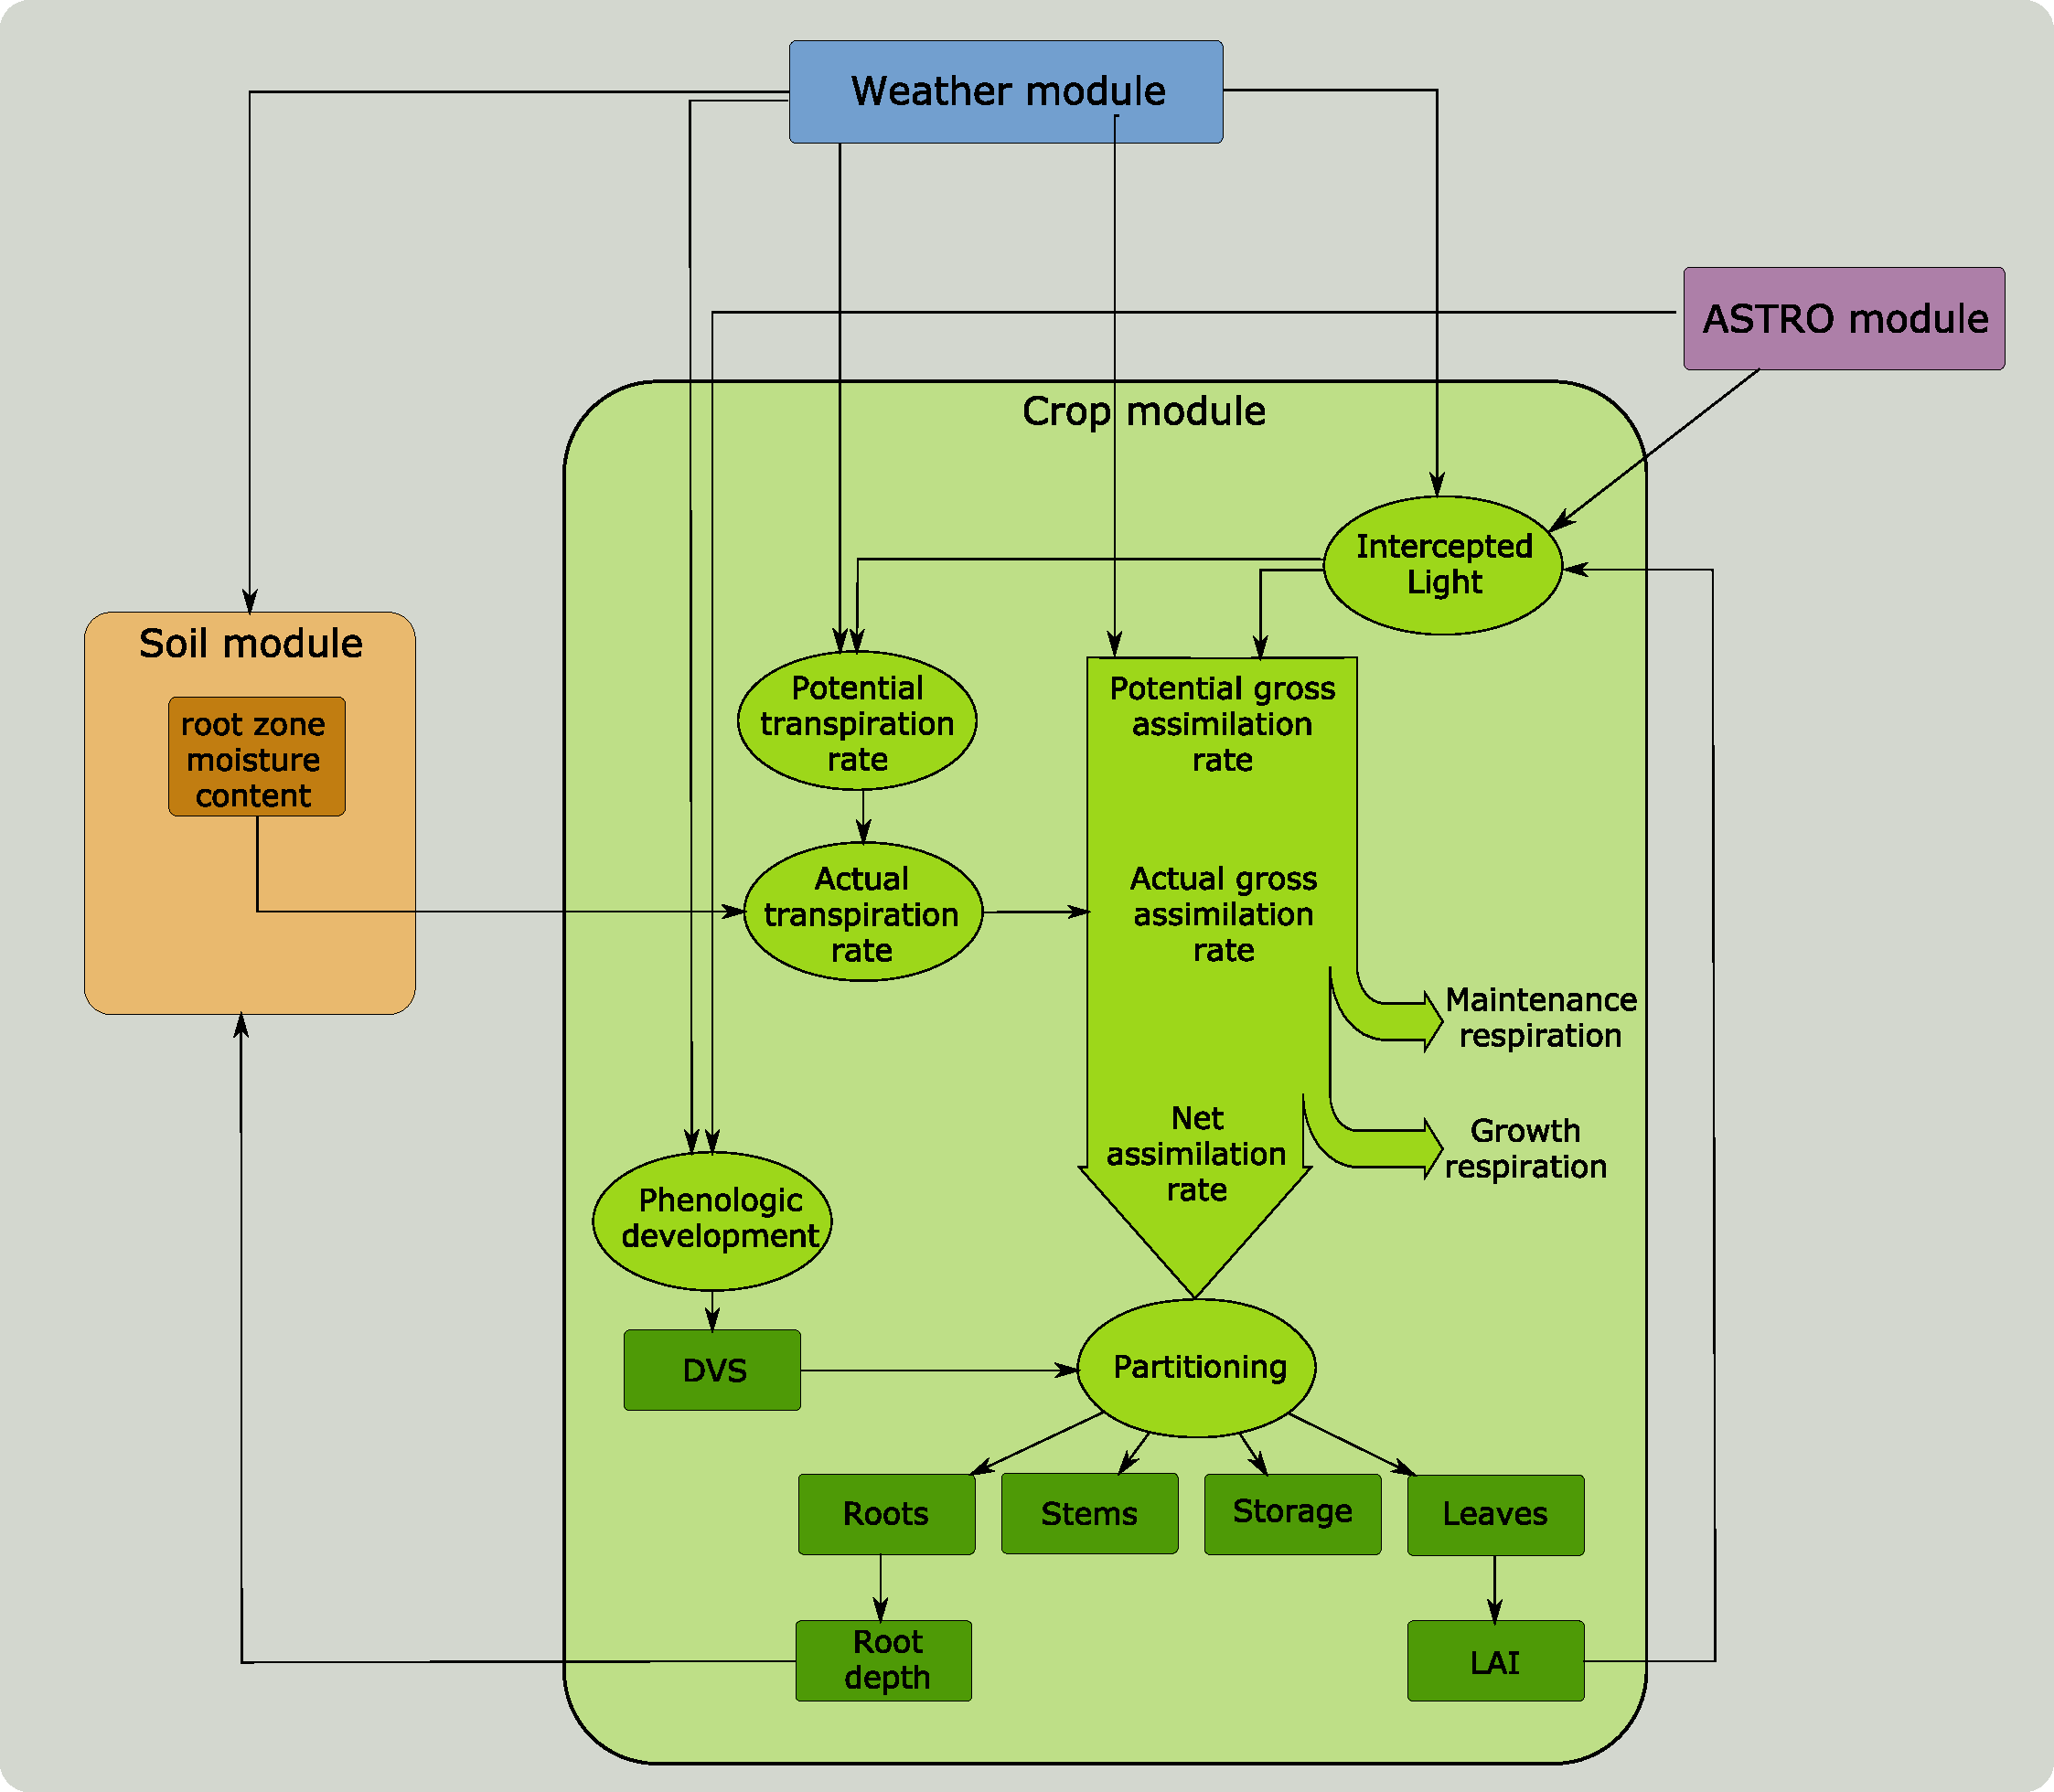
\includegraphics[width=\textwidth ]{\FigDir/wofost_schema_v3.pdf}
	\caption{Schematic overview of the major processes implemented in WOFOST and their linkages.}
	\label{fig:CropGrowthProc2}
\end{figure}

\section{Phenological development of a crop}

The physiological age of a plant is defined by the development stage (DVS), which on its turn is
characterized by the formation of the various organs and their appearance. The most
important phenological change is the one from vegetative to the reproductive stage, which
determines the most important change in the dry matter allocation over organs. As many
physiological and morphological processes change with the phenological stage of the
plant, accurate quantification of phenological development is essential in any simulation
model for crop growth. In WOFOST, the development stage is expressed in a dimensionless variable, 
having the value -0.1 at sowing, 0 at seedling emergence, 1 at flowering and 2 at maturity. 

In recent years the BBCH scale (https://en.wikipedia.org/wiki/BBCH-scale) was developed to provide 
a framework for defining phenological scales for a variety of crops. The phenological stages
used by WOFOST roughly correspond to BBCH scales 0 (sowing), 1 (leaf development), 6 (flowering)
and 9 (senescence). Converting the internal of WOFOST to use the BBCH scale for phenology is 
not trivial because many WOFOST parameters are defined as a function of DVS. Nevertheless,
in calibration studies it was demonstrated that specific DVS values can be linked consistently
to specific BBCH stages. Although the exact DVS values for a crop to reach a specific BBCH
stages can be variety specific.


\subsection{Crop emergence}

As start of the growing season the date of sowing or of emergence can be chosen. For a
photosynthesis-driven model like WOFOST, the simulation of crop growth starts at
emergence. If the sowing date is chosen by the model user, the day of emergence is
determined by the model. The crop emergence can be
defined as a function of the effective daily temperature sum since sowing date. Emergence
takes place when the effective daily temperature sum reaches the threshold temperature
for emergence (acronym: {\bf TSUMEM}). This threshold temperature is crop specific and
should be given by the user. The daily effective temperature depends on the base
temperature {\bf TBASEM}, below which no germination processes take place, and the maximum daily
temperature, beyond which the germination activity does not increase anymore {\bf TEFFMX}.
Both are crop specific. An example of this effective daily temperature as a function of daily
average temperature is depicted in figure \ref{fig:TEFFMAX}.

\begin{figure}[p]
	% fig 5.2
	\centering
	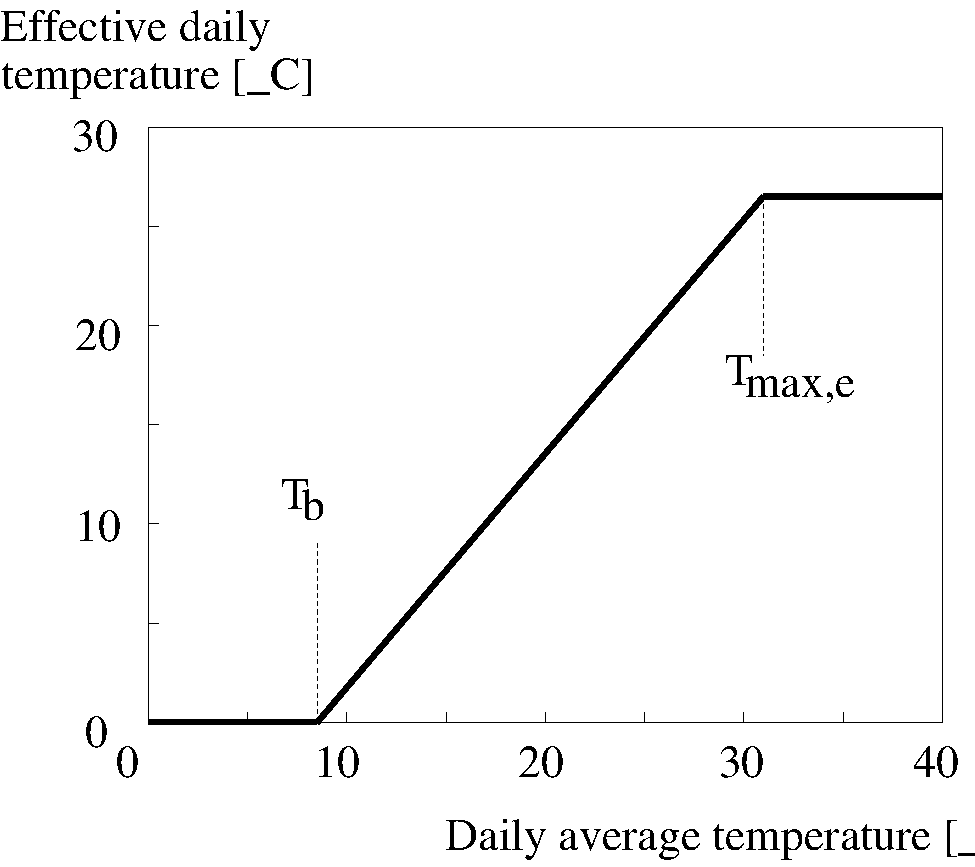
\includegraphics[width=120mm]{\FigDir/TEFFMAX.pdf}
	\caption{Effective temperature from sowing to emergence} 
	\label{fig:TEFFMAX}
\end{figure}

The following relationship can be defined for the effective temperature sum:

\begin{align}
T_{e} &= 0            & T \le T _{b} \nonumber  \\
T_{e} &= T~-~ T _{b}  & T _{b} ~<~T ~ < ~T _{\max ,e} \nonumber  \\
T_{e} &= T _{\max ,e} & T _{b} T \ge  T _{\max \, ,\, e}
\end{align}

Where:\\[5pt]
\begin{tabularx}{\textwidth}{llXr}
	T$_{{\rm e}}$ &:& Effective daily temperature & 
	[\degrees C]\\
	T$_{{\rm max,e}}$ &:& Maximum temperature beyond which phenological 
	activity does not increase    &    [\degrees C]\\
	T$_{{\rm b}}$ &:& Base temperature below which phenological development stops & 
	[\degrees C]\\
	T  &:& (Average) daily temperature & [\degrees C]
\end{tabularx}

Species originating from temperate regions show a base temperature of
0$-$3\degrees C, while species of subtropical and tropical origins have a base temperature of
9$-$14\degrees C (Angus {\it et al.}, 1981). Within a species, cultivars may vary substantially 
in their temperature requirements. The temperature sum, therefore, must be characterized for
each cultivar or group of cultivars (maturity classes).   

\subsection{Phenological development stage}
\label{sec:DVS}

A crop passes through successive phenological development stages. In WOFOST these stages 
are expressed in degree-days and defined by two parameters. The TSUM1 parameter defines
the number of degree-days for the emergence-anthesis period, while the TSUM2 parameter
defines the number of degree-days for the anthesis-maturity period. 
The length of these stages (in days) depends on the development rate. Development rates are 
controlled by vernalization requirements, day length and temperature. In the model before
anthesis, all factors can be active. After anthesis only temperature influence is possible.

Temperature is the main environmental factor affecting the development rate. Higher
temperatures increase the development rate leading to shorter growing periods. This rate
responds to temperature according to a curvilinear relationship. However, it has often
been demonstrated, that over a wide range of temperatures, the development rate
increases more or less linearly with temperature (van Dobben, 1962; van Keulen \&
Seligman, 1987).

In the model a flexible relation is used where the effective increase in temperature
sum, used for the calculation of the development rate, is dependent on the daily temperature 
(Summerfield \& Roberts, 1987). This relation is specified in an AFGEN table, 
allowing to account for non-linearity (lower and upper threshold values and optimum
ranges). The average temperature is the independent variable in the AFGEN table (see
Appendix 2). 

The development rate based on temperature can be reduced by the effect of vernalization and 
day length and can thus be obtained by:

\begin{equation}
% eq 5.3
\label{eq:5.3}
D_{r,t} = {f_{vern}}{f_{dayl}}{\frac{DT_{s}}{\sum T_{i}}}
\end{equation}

Where:\\[5pt]
\begin{tabularx}{\textwidth}{llXr}
	$f_{{\rm vern,t}}$ &:& Reduction factor for vernalization at time step t  & [-]\\
	$f_{{\rm dayl,t}}$ &:& Reduction factor for day length at time step t  & [-]\\
	D$_{{\rm r,t}}$ &:& Development rate at time step t  & [d$^{{\rm -1}}$]\\
	DT$_{{\rm s}}$ &:& Daily effective temperature & [\degrees C]\\
	$\sum$T$_{{\rm i}}$ &:& Temperature sum required to complete stage i & [\degrees C d]\\
\end{tabularx}

The temperature dependent correction factor, {\bf DT$_{{\rm s}}$} (acronym: {\bf DTSMTB}) and 
the temperature sum required to complete stage i, {\bf $\sum$T$_{{\rm i}}$} (acronym: 
{\bf TSUM1} or {\bf TSUM2}) are crop dependent and should be provided by the user.

The development stage at time step t is the integral of the development rate over the time
(i.e. time span from emergence to current time step) and can be calculated according to:

\begin{equation}
\label{eq:5.4}
D_{s,t} ~=~ D_{s,t-1} + D_{r,t} \Delta t
\end{equation}

Where:\\[5pt]
\begin{tabularx}{\textwidth}{llXr}
	D$_{{\rm s,t}}$ &:& Development stage at time step t    &    [-]\\
	D$_{{\rm r,t}}$ &:& Development rate at time step t     &   [d$^{{\rm -1}}$]\\
	$\Delta$t &:& Time step   &     [d]\\
\end{tabularx}

\subsection{Day length}

For certain crops or cultivars, during the vegetative stage (i.e. D$_{{\rm s}}$ $<$ 1), the 
effect of day length should be taken into account (e.g. "photosensitivity"). Moreover, crops 
that are sown in autumn
in temperate climate often require exposure to the prolonged cold of winter in order to be
able to flower. This effect is called the "vernalization requirement" of the crop.

Approaches that describe the effect of day length 
quantitatively are given amongst others by  Weir {\it et al.} (1984), Hadley {\it et al}. (1984) 
and Reinink {\it et al.} (1986). In WOFOST, a reduction factor for the development rate as a 
function of the day length is introduced. In case of photosensitivity can be calculated as:

\begin{equation}
\label{eq:5.5}
f_{red} ~=~{\frac{D ~-~D _{c} }{D _{o} ~-~ D _{c} }} ~~~~~~~~~0~\le ~f _{red} ~\le ~1
\end{equation}

Where:\\[5pt]
\begin{tabularx}{\textwidth}{llXr}
	$f_{{\rm dayl}}$ &:& Development rate reduction factor as function of day length   &     [-]\\
	D &:& Present day length (see eq. \ref{eq:AstroDaylength})   &     [h]\\
	D$_{{\rm c}}$ &:& Critical day length for development (lower threshold)    &    [h]\\
	D$_{{\rm o}}$ &:& Optimum day length for development (upper threshold)    &    [h]\\
\end{tabularx}

The user should provide information whether the development rate depends on temperature, 
on day length or on temperature and day length (acronym: {\bf IDSL}). The critical
daylength, {\bf D$_{{\rm c}}$} (acronym: {\bf DLC}) and the optimum daylength, 
{\bf D$_{{\rm o}}$} (acronym: {\bf DLO}) are crop dependent and should also be provided by 
the user. 

Note that in modern cultivars, photosensitivity is much less pronounced than in traditional
cultivars, and that for the purpose of modelling the day length influence can often be ignored.
However, for winter crops influence of day length and vernalization must be taken into
account in order to avoid that the choice of the sowing date in autumn has a large impact on 
the flowering and maturity date of the crop.


\subsection{Vernalization}

Vernalization is the induction of a plant's flowering process by exposure to the prolonged cold of winter, or by an artificial equivalent. After vernalization, plants have acquired the ability to flower, but they may require additional seasonal cues or weeks of growth before they will actually flower (source: Wikipedia). 

In WOFOST vernalization is simulated by assuming that a crop requires a number of (cultivar-specific)
vernalization days in order to reach its vernalization requirement. One vernalization day is added to the 
vernalization state 
when the daily average temperature is within the optimal temperature range for vernalization. A fractional
day or zero  is added when the temperature is outside of this range. This is rate of vernalization
(acronym: {\bf VERNR}) is decribed using an AFGEN table (acronym:  {\bf VERNRTB}) which describes the
temperature response curve for vernalization (figure ???).

The reduction factor on development rate is than derived by linearly scaling the current vernalization state 
((acronym:  {\bf VERN}))  between a base vernalization ((acronym:  {\bf VERNBASE})) and the number of 
days required to saturate the vernalization requirement (acronym:  {\bf VERNSAT}). The reduction 
factor can thus be expressed as: 

\begin{equation}
\label{eq:vern_factor}
f_{vern} ~=~{\frac{V ~-~V_{base} }{V _{sat} ~-~ V_{base} }} ~~~~~~~~~0~\le ~f _{vern} ~\le ~1
\end{equation}

Where:\\[5pt]
\begin{tabularx}{\textwidth}{llXr}
	$f_{{\rm vern}}$ &:& Development rate reduction factor as function of vernalization state   &     [-]\\
	$V$ &:& Present vernalization state of the crop   &     [days]\\
	$V_{{\rm base}}$ &:& Base vernalization for development (lower threshold)    &    [days]\\
	$V_{{\rm sat}}$ &:& Saturated vernalization for development (upper threshold)    &    [days]\\
\end{tabularx}

Note that it is possible for crops under certain conditions to de-vernalize, but this effect is not taken
into account in WOFOST.

\subsection{End of the crop cycle}

The simulation of crop growth stops when the development stage reaches the stage at
which the crop will be harvested (acronym: {\bf DVSEND}). For crops that are harvested
at maturity {\bf DVSEND}) will be equal to 2.0. However, for crops that are deliberately
harvested earlier (e.g. silage maize) the value can be lower. For crops that are harvested
at a defined date, the value for {\bf DVSEND}) will be ignored.

\section{Daily assimilation} 

Daily dry matter production is the most detailed part of the model. The following steps
can be distinguished and will be described separately:
\begin{itemize}
	\item Total instantaneous gross CO$_{{\rm 2}}$ assimilation of the canopy 
	[\S \ref{sec:InstantGrossAssimilation}]
	\item Total daily gross CO2 assimilation rate of the canopy 
    [\S \ref{sec:DailyGrossAssimilation}]
	\item Actual daily gross photosynthesis rate of the canopy
	including temperature and development stage effect
    [\S \ref{sec:DailyGrossPhotosynthesis}]
	\item Reductions due to water and nutrient shortages
    [\S \ref{sec:PhotosynthesisReductionFactors}]
\end{itemize}

The daily rate of CO$_{{\rm 2}}$ assimilation of the crop is driven by the intercepted light and can
be obtained by integrating the total instantaneous CO$_{{\rm 2}}$ assimilation rate of the canopy over
the day. The total instantaneous assimilation rate is calculated in subroutine {\bf ASSIM}, the
integration of the total instantaneous assimilation rate in subroutine {\bf TOTASS}. Both
calculations make use of the 3-point Gaussian integration method for calculating daily total 
gross assimilation (Goudriaan, 1986; Spitters, 1986).
Finally, actual gross photosynthesis is computed by applying correction factors for temperature,
water stress and nutrient stress onto the total daily assimilation

\subsection{Total daily gross CO$_{{\rm 2}}$ assimilation rate of the canopy}
\label{sec:DailyGrossAssimilation}

To calculate the total daily gross CO$_{{\rm 2}}$ assimilation rate of the whole canopy, an integration over time should be performed. Therefore, for given fluxes of photosynthetically
active radiation, at three different periods of the day, the total instantaneous gross canopy
CO$_{{\rm 2}}$ assimilation rate is computed. Afterwards, the integral of the total instantaneous
gross canopy CO$_{{\rm 2}}$ assimilation rate over time, as a weighted average of the selected three
hours, is calculated (Gaussian integration, see Appendix 1).

For the calculation of the total instantaneous gross canopy CO$_{{\rm 2}}$ assimilation rate, an
integration over depth of the gross instantaneous assimilation rate has to be performed.
Therefore, at three different depths in the canopy the gross instantaneous assimilation rate
is calculated, whereafter the integral of the gross instantaneous assimilation rate over
depth, as a weighted average of the selected depths, is computed (Gaussian integration,
see Appendix 1)

Integration, to calculate the daily total assimilation, is only necessary if instantaneous
assimilation will take place. Instantaneous assimilation will be zero if the leaf area index
equals zero (no photosynthetic activity). A second restriction for the integration is the
maximum CO$_{{\rm 2}}$ assimilation rate as a function of development stage, which is crop
dependent. When this maximum assimilation rate at light saturation equals zero also no
instantaneous assimilation will take place and no integration has to be performed.

As is mentioned before, in order to integrate the gross instantaneous assimilation rate
over the day, three points in time are selected to calculate the photosynthetically active
radiation. In this particular case, the radiation is homogeneously distributed over the day
according to the sine of the solar elevation, so the weighted average CO$_{{\rm 2}}$ 
assimilation rate can therefore be calculated for half a day only.

The three points in time are selected from noon to sunset (this explains the use of the
constants 0.5 and 12.00):

\begin{equation}
% eq 5.6
t_{h} = 12 + 0.5 \cdot D \cdot (0.5 ~+~ p\, \sqrt{0.15}) ~~~ for ~~~ p = -1,0,1
\end{equation}

Where:\\[5pt]
\begin{tabularx}{\textwidth}{llXr}
	D &:& Day length (see eq. \ref{eq:AstroDaylength})    &    [h]\\
	t$_{{\rm h}}$ &:& Hour of the day  &      [h]\\
	p &:& Gaussian integration points  &      [-]\\
\end{tabularx}

The incoming radiation and therefore gross assimilation rate, changes with solar elevation. 
The solar height as a function of the hour of the day can be calculated with:

\begin{equation}
\label{eq:5.7}
\sin \beta ~=~ \sin \lambda \, \sin \sigma ~+~ \cos \lambda \, \cos \sigma \, \cos \, 
(\, 2 \pi \,{\frac{t _{h} ~+~ 12}{24}} )
\end{equation}


Where:\\[5pt]
\begin{tabularx}{\textwidth}{llXr}
	$\beta$ &:& Solar elevation   &    [degrees]\\
	$\sigma$ &:& Solar declination    &    [degrees]\\
	$\lambda$ &:& Latitude     &   [degrees]\\
	t$_{{\rm h}}$ &:& Hour of the day    &    [h]\\
\end{tabularx}

Measured or estimated daily global solar radiation  (wavelength 300 - 3000 nm) is input
in the model. Only half of this incoming radiation is photosynthetically active (PAR,
Photosynthetically Active Radiation, wavelength 400 - 700 nm). This fraction, which is
generally called 'light' or 'visible radiation', is used in the calculation procedure of the
CO$_{{\rm 2}}$ assimilation rate of the canopy. In the model, the instantaneous incoming 
photosynthetically active radiation is calculated by multiplying half of the daily global radiation
with the ratio of the actual effective solar elevation and the integral of the effective solar
height (see also eq. \ref{eq:IntSolarHeight}):

\begin{equation}
\label{eq:5.8}
I _{0} ~=~ 0.5\, S _{g,d} \,{\frac{\sin \beta \, (\, 1~+~0.4\, \sin \beta \, )}{\int \, \sin \beta _{m} }}
\end{equation}

Where:\\[5pt]
\begin{tabularx}{\textwidth}{llXr}
	I$_{{\rm 0}}$ &:& Photosynthetically active radiation flux    &    
	[J m$^{{\rm -2}}$ s$^{{\rm -1}}$]\\
	S$_{{\rm g,d}}$ &:& Daily global radiation   &     
	[J m$^{{\rm -2}}$ d$^{{\rm -1}}$] \\
	$\beta$ &:& Solar elevation    &    [degrees]\\
	$\int \sin \beta_{{\rm m}}$ &:& The corrected integral of solar height over the day 
	for non homogeneous atmospheric transmission (eq. \ref{eq:IntSolarHeight})   
	&     [s]\\
\end{tabularx}

The calculated photosynthetically active radiation flux consists of a diffuse flux and a
direct flux. The diffuse flux is the result of scattering of sun rays by clouds, aerosols and
gases in the atmosphere. The proportion of diffuse light in the total incident light flux
depends on the status of the atmosphere (see also eq. \ref{eq:irrad_diffuse}). This fraction 
is calculated from the atmospheric transmission using an empirical function (Spitters 
{\it et al.}, 1986).

\begin{equation}
% eq 5.9
I_{0,df} ~=~ D _{p~} \sin \beta
\end{equation}

Where:\\[5pt]
\begin{tabularx}{\textwidth}{llXr}
	I$_{{\rm 0,df}}$ &:& Diffuse part of the photosynthetically active radiation flux 
	at top of the canopy    &    [J m$^{{\rm -2}}$ s$^{{\rm -1}}$]\\
	D$_{{\rm p}}$ &:& Diffuse radiation perpendicular to the direction 
	light (see eq. 4.31)    &    [J m$^{{\rm -2}}$ s$^{{\rm -1}}$]\\
	sin$\beta$ &:& Solar elevation (see eq. \ref{eq:5.7})    &    [degrees]\\
\end{tabularx}

The direct part can be easily obtained by subtracting the diffuse part from the
photosynthetically radiation flux:

\begin{equation}
% eq 5.10
I_{0,dr} ~=~ I_{0} ~-~I_{0,df} 
\end{equation}

Where:\\[5pt]
\begin{tabularx}{\textwidth}{llXr}
	I$_{{\rm 0,dr}}$ &:& Direct part of the photosynthetically active radiation flux 
	at top of the canopy    &    [J m$^{{\rm -2}}$ s$^{{\rm -1}}$]\\
	I$_{{\rm 0}}$ &:& Photosynthetically active radiation flux (see eq. \ref{eq:5.8})    &  
	[J m$^{{\rm -2}}$ s$^{{\rm -1}}$]\\
	I$_{{\rm 0,df}}$ &:& Diffuse part of the photosynthetically active radiation flux 
	at top of the canopy     &   [J m$^{{\rm -2}}$ s$^{{\rm -1}}$]\\
\end{tabularx}

Once the photosynthetically active radiation fluxes have been established, the 
instantaneous gross assimilation rate of the canopy can be calculated (see \S
\ref{sec:InstantGrossAssimilation}). And the integration over time can take place.
The integral of the total gross canopy assimilation rate over time is calculated as the
weighted average of the three selected hours of the day. Multiplying by the day length
results in the total daily gross rate of CO$_{{\rm 2}}$ assimilation. 

\begin{equation}
\label{eq:5.11}
A_{d} = D {\frac{A_{C,-1} ~+~ 1.6 A_{C,0} ~+~ A_{C,1} }{3.6}}
\end{equation}

Where:\\[5pt]
\begin{tabularx}{\textwidth}{llXr}
	A$_{{\rm d}}$ &:& Total gross assimilation rate    &    
	[kg ha$^{{\rm -1}}$ d$^{{\rm -1}}$]\\
	D &:& Day length (see eq. \ref{eq:AstroDaylength})   &     [h]\\
	A$_{{\rm C}}$ &:& Total inst. gross assimilation rate for
	the whole canopy, p= -1,0,1 (see eq. \ref{eq:5.31})    &
	[kg ha$^{{\rm -1}}$ h$^{{\rm -1}}$]\\
\end{tabularx}

\subsection{Total instantaneous gross CO$_{2}$ assimilation of the canopy}  
\label{sec:InstantGrossAssimilation}

In the subroutine {\bf ASSIM}, the total instantaneous rate of CO$_{{\rm 2}}$ assimilation of the canopy is
calculated from the incoming fluxes of diffuse and direct photosynthetic active radiation,
solar elevation and leaf area index and several parameters.

\subsubsection{Reflection and extinction}
The total incoming photosynthetically active radiation flux is partly reflected by the
canopy. The reflection coefficient is defined as the fraction of the downward radiation
flux that is reflected by the whole canopy. According to Goudriaan (1977), the reflection
coefficient of a green leaf canopy with a random spherical leaf angle equals:

\begin{equation}
\label{eq:5.12}
\rho = {\frac{1- \sqrt{1-\sigma}}{1 + \sqrt{1-\sigma}}} \cdot {\frac{2}{1+1.6 \sin \beta }}
\end{equation}

Where:\\[5pt]
\begin{tabularx}{\textwidth}{llXr}
	$\rho$ &:& Reflection coefficient of a green leaf canopy    &    [-]\\
	$\sigma$ &:& Scattering coefficient fraction (transmission and reflection) 
	of single leaves for visible radiation   
	{\small (=0.2; Goudriaan, cited by Spitters, 1986)}  &     [-]\\  
	$\beta$ &:& Solar elevation (see eq. \ref{eq:SolarElevation})    &    [degrees]\\
\end{tabularx}

The first term denotes the reflection of the canopy of horizontal leaves and the second
term is the approximate correction factor for a spherical leaf angle distribution.

A fraction (1-$\rho$) of the incoming visible radiation is potentially available for absorption by
the canopy. Radiation fluxes attenuate exponentially within a canopy with increasing leaf
area from the top downwards:

\begin{equation}
\label{eq:5.13}
I_{L~} = I_{0} (1~-~\rho ) e^{-\kappa LAI_{L} }
\end{equation}

Where:\\[5pt]
\begin{tabularx}{\textwidth}{llXr}
	I$_{{\rm L}}$   &:& Net photosynthetic active radiation flux at 
	depth L in the canopy    &    [J m$^{{\rm -2}}$ s$^{{\rm -1}}$]\\
	I$_{{\rm 0}}$   &:& Photosynthetically active radiation flux (see eq. \ref{eq:5.8})  & 
	[J m$^{{\rm -2}}$ s$^{{\rm -1}}$]\\
	LAI$_{{\rm L}}$ &:& Cumulative leaf area index (from top downwards) 
	relative depth L & [ha ha$^{{\rm -1}}$]\\
	$\rho$          &:& Reflection coefficient of the canopy   &     [-]\\
	$\kappa$        &:& Extinction coefficient for photosynthetic active 
	radiation flux   &     [-]\\
\end{tabularx}

The diffuse and the direct flux have different extinction coefficients, giving rise to
different light profiles within the canopy for diffuse and direct radiation. Therefore three
different radiation fluxes are distinguished:
\begin{itemize}
	\item the diffuse flux, with extinction coefficient $\kappa_{df}$;
	\item the total direct flux, with extinction coefficient $\kappa_{dr,t}$;
	\item the direct component of direct light, with extinction coefficient $\kappa_{dr,bl}$.
\end{itemize}

Radiation becomes diffuse when sun rays are partly absorbed and partly scattered (i.e.
reflected or transmitted) by a leaf. The subscript {\it bl} (black) is used, the leaves show
neither transmission nor reflection. The extinction coefficient of 'black leaves'
can be calculated as:

\begin{equation}
% eq 5.14
\label{eq:5.14}
\kappa_{bl} ~=~{\frac{0.5}{\sin \beta }}
\end{equation}

Where:\\[5pt]
\begin{tabularx}{\textwidth}{llXr}
	$\kappa$$_{{\rm bl}}$ &:& Extinction coefficient for the direct radiation flux   &     [-]\\
	$\beta$ &:& Solar elevation    &    [degree]\\
\end{tabularx}

For a spherical leaf area distribution (homogeneous, random), the extinction coefficient
for the diffuse radiation flux equals:

\begin{equation}
\label{eq:5.15}
\kappa_{df} ~=~ \kappa_{bl} \, \sqrt{1~-~ \sigma }
\end{equation}

Where:\\[5pt]
\begin{tabularx}{\textwidth}{llXr}
	$\kappa$$_{{\rm df}}$ &:& Extinction coefficient for the diffuse radiation flux    &    [-]\\
	$\sigma$ &:& Scattering coefficient fraction of single leaves for 
	visible radiation    &    [-]\\
\end{tabularx}

In the model, the extinction coefficient for the diffuse radiation flux, 
{\bf $\kappa$$_{{\rm df}}$} (acronym: {\bf KDIF})
is not computed but should be provided by the user. It can be measured directly 
under diffuse sky conditions.

In equation \ref{eq:5.14}, 0.5 points to the average projection on the ground surface of leaves
showing a spherical angle distribution, and 0.8 in equation \ref{eq:5.16} is the value of 0.5/sin$\beta$
averaged over elevation $\beta$ of incident radiation under an overcast sky.

The average extinction coefficient for the diffuse radiation flux is about 0.72 (Goudriaan,
1977). However, in many situations, the leaf angle distribution is not spherical. For
example in rice, the leaves are clustered (especially in the beginning as a result of
planting on hills), and have a very vertical orientation. Other leaf angle distributions can
be accounted for by a procedure described by Goudriaan (1986), which calculates the
extinction coefficient for the diffuse radiation flux on the basis of the frequency 
distribution of leaves with angles in different classes.

In the model however, the leaf angle distribution is accounted for by using a so called
cluster factor which is the measured extinction coefficient for diffuse radiation flux,
relative to the theoretical one for a spherical leaf area distribution. The cluster factor can
be calculated as: 

\begin{equation}
\label{eq:5.16}
C _{f} ~=~{\frac{ \kappa _{df} }{0.8\, \sqrt{1 ~-~ \sigma } }}
\end{equation}

Where:\\[5pt]
\begin{tabularx}{\textwidth}{llXr}
	C$_{{\rm f}}$ &:& Cluster factor    &    [-]\\
	$\kappa$$_{{\rm df}}$ &:& Extinction coefficient for diffuse radiation flux   &     [-]\\
	$\sigma$ &:& Scattering coefficient fraction of single leaves for
	visible radiation  &      [-]\\
\end{tabularx}

The direct component can be calculated as (Goudriaan, 1977):

\begin{equation}
\label{eq:5.17}
\kappa _{dr,bl} ~=~{ C _{f} }\,{\frac{0.5}{\sin \beta }}
\end{equation}

Where:\\[5pt]
\begin{tabularx}{\textwidth}{llXr}
	$\kappa$$_{{\rm dr,bl}}$ &:& Extinction coefficient for the direct component of direct light   &     [-] \\
	C$_{{\rm f}}$ &:& Cluster factor     &   [-]\\
	$\beta$ &:& Solar elevation     &   [degrees]\\
\end{tabularx}

The extinction coefficient for the total direct radiation flux can be calculated as (Goudriaan, 1977):

\begin{equation}
\label{eq:5.18}
\kappa _{dr,t} ~=~ \kappa _{dr,bl} \sqrt{1~-~\sigma }
\end{equation}

Where:\\[5pt]
\begin{tabularx}{\textwidth}{llXr}
	$\kappa_{dr,t}$ &:& Extinction coefficient for total direct radiation flux   &    [-]\\
	$\kappa_{dr,bl}$ &:& Extinction coefficient for the direct component of direct light  &   [-]\\
	$\sigma$ &:& Scattering coefficient     &    [-]\\
\end{tabularx}

\subsubsection{Absorption}
Three depths in the canopy are selected according to the Gaussian integration method (see
Appendix 1) and at those levels the leaf area index, the amount of absorbed radiation and
the leaf CO$_{{\rm 2}}$ assimilation is calculated. The total instantaneous assimilation is easily
obtained by multiplying the instantaneous assimilation with the total leaf area index (eq.
\ref{eq:5.31}). In the following text the calculation processes, concerning the instantaneous
assimilation, will be explained in detail. Calculation of the leaf area index will be
explained in \S \ref{sec:5.4.5}.

Canopy assimilation is calculated as a weighted average of the assimilation at three
horizons within the canopy. The leaf area index of the selected horizons can be written as
(Goudriaan, 1986):

\begin{equation}
% eq 5.19 a-d
LAI_{L} = (0.5 + p \sqrt{0.15}) \cdot LAI~~~~for~~~~p = -1,0,1
\end{equation}


Where:\\[5pt]
\begin{tabularx}{\textwidth}{llXr}
	LAI$_{{\rm L}}$ &:& Leaf area index at relative distance L in the canopy 
	(L=0 at the top)    &    [ha ha$^{{\rm -1}}$]\\
\end{tabularx}

The light absorbed at a certain depth in the canopy is obtained by taking the derivative of
equation \ref{eq:5.13} with respect to the cumulative leaf area index:

\begin{equation}
% eq 5.20
I_{a,L} = {\frac{-dI _{0\, ,\, L} }{dL}} = \kappa (1 -  \rho) I_{0} \cdot e^{- \kappa LAI_{L}}
\end{equation}

Where:\\[5pt]
\begin{tabularx}{\textwidth}{llXr}
	I$_{{\rm a,L}}$ &:& Amount absorbed of total radiation flux
	\footnote{With the 'Total radiation flux' in this paragraph the total photosynthetically 
		active radiation flux is meant.} at relative depth L    &    
	[J m$^{{\rm -2}}$ s$^{{\rm -1}}$]\\
	I$_{{\rm 0,L}}$ &:& Net photosynthetic active radiation at relative depth L in 
	the canopy    &    [J m$^{{\rm -2}}$ s$^{{\rm -1}}$]\\
	I$_{{\rm 0}}$ &:& Photosynthetically active radiation flux at top of the 
	canopy   &     [J m$^{{\rm -2}}$ s$^{{\rm -1}}$]\\
	L &:& Relative depth in the canopy   &     [-]\\
	$\kappa$ &:& The extinction coefficient for the PAR flux    &     [-]\\
	$\rho$ &:& Reflection coefficient of the canopy (see eq. \ref{eq:5.12})   &     [-]\\
\end{tabularx}

If expressed for the different light components, the absorbed fluxes for the different
components per unit leaf area at a certain depth in the canopy are:

\stepcounter{equation}
\begin{align}
% equation 5.21a-c
I_{a,df} &={\frac{-dI_{df,L}}{dL}} &
&= \kappa_{df} (1 - \rho)\, I_{0,df} \cdot e^{-\kappa_{df} \, LAI_{L}} \subeqn  \\
I_{a,dr,t} &= {\frac{-dI_{dr,t,L}}{dL}} & 
&= \kappa_{dr,t} (1-\rho) I_{0,dr} \cdot e^{-\kappa_{dr,t} LAI_{L}} \subeqn  \\
% TODO: check if below I_{a,dr,dr} should be changed to I_{a,dr,bl}
I_{a,dr,dr} &= {\frac{-dI_{dr,L}}{dL}} &
&= \kappa_{dr,bl} (1-\sigma) I_{0,dr} \cdot e^{-\kappa_{dr,bl} LAI_{L}} \subeqn
\end{align}

Where:\\[5pt]
\begin{tabularx}{\textwidth}{llXr}
	I$_{{\rm a,.}}$ &:& Amount absorbed of specified radiation flux   &      
	[J m$^{{\rm -2}}$ s$^{{\rm -1}}$]\\
	I$_{{\rm .,L}}$ &:& Net specified component of PAR flux at relative depth L    &    
	[J m$^{{\rm -2}}$ s$^{{\rm -1}}$]\\
	I$_{{\rm 0}}$ &:& Photosynthetically active radiation flux at top of the canopy
	(see eq. \ref{eq:5.8})   &   [J m$^{{\rm -2}}$ s$^{{\rm -1}}$]\\
	L &:& Relative depth in the canopy   &     [-]\\
	$\kappa$$_{{\rm .}}$ &:& The extinction coefficient for specified radiation 
	(see eq. \ref{eq:5.15}, \ref{eq:5.17} and \ref{eq:5.18})    &    [-]\\
	$\rho$ &:& Reflection coefficient of the canopy (see eq. \ref{eq:5.12})   &     [-]\\
	$\sigma$ &:& Scattering coefficient    &    [-]\\
	bl &:& Black &\\
	df &:& Diffuse &\\
	dr &:& Direct &\\
	t &:& Total &\\
\end{tabularx}

Note that of the direct component of the direct flux the non-scattered part (1-$\sigma$) is
absorbed.

The total absorbed flux for shaded leaves can be calculated as the sum of the absorbed
flux of diffuse radiation and absorbed flux of the diffuse radiation of the indirect
component of direct radiation. The last one is equal to the difference of the absorbed flux
of the total radiation minus the absorbed flux of the direct component of the direct
radiation.

\begin{equation}
\label{eq:5.22}
I _{a,sh} ~=~ I _{a,df} ~+~ (I_{a,dr,t} ~-~ I_{a,dr,dr} )
\end{equation}

Where:\\[5pt]
\begin{tabularx}{\textwidth}{llXr}
	I$_{{\rm a,sh}}$ &:& Absorbed amount of the total radiation flux by shaded leaves
	&    [J m$^{{\rm -2}}$ s$^{{\rm -1}}$]\\
	I$_{{\rm a,df}}$ &:& Absorbed amount of the diffuse radiation flux
	&     [J m$^{{\rm -2}}$ s$^{{\rm -1}}$]\\
	I$_{{\rm a,dr,t}}$ &:& Absorbed amount of the total direct radiation flux
	&     [J m$^{{\rm -2}}$ s$^{{\rm -1}}$]\\
	I$_{{\rm a,dr,dr}}$ &:& Absorbed amount of direct component of the  direct radiation flux
	& [J m$^{{\rm -2}}$ s$^{{\rm -1}}$]\\
\end{tabularx}


\subsubsection{Instantaneous gross assimilation}
The CO$_{{\rm 2}}$ assimilation-light response can be obtained by introducing the absorbed amount
of light into an assimilation-light response function of individual leaves. This assimilation-light
response curve is computed using an exponential function that requires the instantaneous assimilation 
rate at light saturation and the initial angle to be defined:

\begin{equation}
\label{eq:5.23}
A_{L} = A_{m} (1-\exp({{-\epsilon I_{a}}/{A_{m}}}))
\end{equation}

Where:\\[5pt]
\begin{tabularx}{\textwidth}{llXr}
	A$_{{\rm L}}$ &:& Inst.\footnote{ Inst. = Instantaneous} gross assimilation 
	rate at relative depth L (per unit leaf area)    &    
	[kg ha$^{{\rm -1}}$ h$^{{\rm -1}}$]\\
	A$_{{\rm m}}$ &:& Inst. gross assimilation rate at light saturation    & 
	[kg ha$^{{\rm -1}}$ h$^{{\rm -1}}$]\\
	$\epsilon$ &:& Initial light use efficiency   &   [(kg ha$^{{\rm -1}}$ 
	h$^{{\rm -1}}$)/(J m$^{{\rm -2}}$ s$^{{\rm -1}}$])\\
	I$_{{\rm a}}$ &:& Absorbed amount of the total radiation flux     &   
\end{tabularx}

The instantaneous gross assimilation rate at light saturation, {\bf A$_{{\rm m}}$} (acronym: {\bf AMAXTB}) is
crop specific. It is a function of the crop development stage and corrected for the ambient CO$_{2}$ 
concentration (acronym: {\bf CO2AMAXTB}). The initial light use efficiency, {\bf $\epsilon$}
(acronym: {\bf EFFTB}), is also crop dependent. It is defined as a function of daily mean temperature and
corrected for ambient CO2 concentration ((acronym: {\bf CO2EFFTB})). 

Introducing the absorbed amount of radiation by shaded leaves (eq. \ref{eq:5.22}) into 
equation \ref{eq:5.23} yields:

\begin{equation}
\label{eq:5.24}
A_{sh} = A_{m} \big(1-\exp({{-\epsilon I_{a,sh} }/{A_m}} ) \big)
\end{equation}

Where:\\[5pt]
\begin{tabularx}{\textwidth}{llXr}
	A$_{{\rm sh}}$ &:& Inst. gross assimilation rate for shaded leaves  & 
	[kg ha$^{{\rm -1}}$ h$^{{\rm -1}}$]\\
	A$_{{\rm m}}$ &:& Inst. gross assimilation rate at light saturation & 
	[kg ha$^{{\rm -1}}$ h$^{{\rm -1}}$]\\
	$\epsilon$ &:& Initial light use efficiency  &  
	[(kg ha$^{{\rm -1}}$ h$^{{\rm -1}}$)/(J m$^{{\rm -2}}$ s$^{{\rm -1}}$)]\\
	I$_{{\rm a,sh}}$ &:& Absorbed amount of the total radiation flux  by shaded leaves (see eq. \ref{eq:5.22})   &
	[J m$^{{\rm -2}}$ s$^{{\rm -1}}$]\\
\end{tabularx}

For the sunlit leaf area, the average absorption intensity may be substituted in equation
\ref{eq:5.23}. However, it is more accurate to account for the variation in leaf angle and thus in
illumination intensity (Spitters, 1986). The direct flux is absorbed by a leaf perpendicular
to the direct beam with an intensity of: 

\begin{equation}
\label{eq:5.25}
I_{a,dr,sl} = {\frac{(1-\sigma) I_{0,dr}}{\sin \beta }}
\end{equation}

Where:\\[5pt]
\begin{tabularx}{\textwidth}{llXr}
	I$_{{\rm a,dr,sl}}$ &:& Absorbed amount of the direct radiation flux by leaves
	perpendicular to the direct beam    &    [J m$^{{\rm -2}}$ s$^{{\rm -1}}$]\\
	I$_{{\rm 0,dr}}$ &:& Direct flux of visible radiation at the top of 
	the canopy &  [J m$^{{\rm -2}}$ s$^{{\rm -1}}$]\\
	$\sigma$ &:& Scattering coefficient  &[-]\\
	$\beta$ &:& Solar elevation   & [degrees]\\
\end{tabularx}

The amount of absorbed direct radiation by leaves (eq. \ref{eq:5.25}) depends on the sine of
incidence at the leaf surfaces. Therefore, for sunlit leaves, CO$_{{\rm 2}}$ assimilation rates have to
be calculated separately for leaves with different angles and integrated over the sine of
incidence. In the model a spherical leaf angle distribution is assumed, so no integration
over leaf angles is needed.

Integration over the sine of incidence for the sunlit leaves yields (Goudriaan, personal
communication):

\begin{equation}
% eq 5.26
A_{sl} = A_{m} \bigg( 
1-(A_{m} - A_{sh})  {\frac{1~- \exp({{-I _{a,dr,sl} \, \epsilon}}/{A_m}) }
	{\epsilon\, I _{a,dr,sl} }}
\bigg)
\end{equation}

Where:\\[5pt]
\begin{tabularx}{\textwidth}{llXr}
	A$_{{\rm sl}}$ &:& Inst. gross assimilation rate for sunlit leaves  &
	[kg ha$^{{\rm -1}}$ h$^{{\rm -1}}$]\\
	A$_{{\rm sh}}$ &:& Inst. gross assimilation rate for shaded leaves  &
	[kg ha$^{{\rm -1}}$ h$^{{\rm -1}}$]\\
	A$_{{\rm m}}$ &:& Inst. gross assimilation rate at light saturation &
	[kg ha$^{{\rm -1}}$ h$^{{\rm -1}}$]\\
	I$_{{\rm a,dr,sl}}$ &:& Absorbed amount of the direct radiation flux by leaves
	perpendicular to the direct beam  &  [J m$^{{\rm -2}}$ s$^{{\rm -1}}$]\\
	$\epsilon$ &:& Initial light use efficiency  &   [(kg ha$^{{\rm -1}}$ 
	h$^{{\rm -1}}$)/(J m$^{{\rm -2}}$ s$^{{\rm -1}}$)]\\
\end{tabularx}

The assimilation rate per unit leaf area at a specific depth in the canopy is the sum of the
assimilation rates of sunlit and shaded leaves, taking into account the proportion of sunlit
and shaded leaf area at that depth in the canopy. 

The fraction sunlit leaf area equals the fraction of the direct radiation reaching that layer:

\begin{equation}
% eq 5.27
f_{sl} =  e^{-\kappa_{dr,bl} \cdot LAI_{L}}
\end{equation}

Where:\\[5pt]
\begin{tabularx}{\textwidth}{llXr}
	f$_{{\rm sl}}$ &:& Fraction sunlit leaf area   &     [-]\\
	$\kappa$$_{{\rm dr,bl}}$ &:& Extinction coefficient for the direct component of
	direct radiation (see eq. \ref{eq:5.17})   &     [-]\\
	LAI$_{{\rm L}}$ &:& Cumulative leaf area index at relative depth L in canopy  &      [-]
\end{tabularx}

The total instantaneous assimilation rate at a relative depth L can be calculated as:

\begin{equation}
\label{eq:5.28}
A_{T,L} = f_{sl} A_{sl} + (1 - f_{sl}) A_{sh} 
\end{equation}

Where:\\[5pt]
\begin{tabularx}{\textwidth}{llXr}
	A$_{{\rm T,L}}$ &:& Total inst. gross assimilation rate at a relative depth L   &
	[kg ha$^{{\rm -1}}$ h$^{{\rm -1}}$]\\
	A$_{{\rm sl}}$ &:& Inst. gross assimilation rate for sunlit leaves  & 
	[kg ha$^{{\rm -1}}$ h$^{{\rm -1}}$]\\
	A$_{{\rm sh}}$ &:& Inst. gross assimilation rate for shaded leaves  & 
	[kg ha$^{{\rm -1}}$ h$^{{\rm -1}}$]\\
	f$_{{\rm sl}}$ &:& Fraction sunlit leaf area  &  [-]\\
\end{tabularx}

The total instantaneous assimilation rate for the whole canopy per unit leaf area can be
established using the Gaussian integration method, as a weighted average of the assimilation 
at three levels within the canopy.
However, first the leaf area index of the levels selected have to be established:

\begin{equation}
\label{eq:5.29}
LAI_{L} = (0.5+p \sqrt{0.15})LAI~~~~for~~~~p=-1,0,1
\end{equation}

Where:\\[5pt]
\begin{tabularx}{\textwidth}{llXr}
	LAI$_{{\rm L}}$ &:& Leaf area index at relative depth L in canopy    &    [ha ha$^{{\rm -1}}$]\\
	LAI &:& Total leaf area of the crop (see \S \ref{sec:5.4.5}) &   [ha ha$^{{\rm -1}}$]\\
\end{tabularx}

Introducing the values of the leaf area index of the three selected layers in the equations
mentioned before, will yield the instantaneous assimilation at these horizons. The
weighted average of these values yields the total instantaneous assimilation rate for the
whole canopy per unit leaf area.

The weighted average of the total instantaneous assimilation rates can be calculated as:

\begin{equation}
% eq 5.30
A_{C,l} = {\frac{(A_{T,L,-1} + 1.6 A_{T,L,0} + A_{T,L,1})}{3.6}}
\end{equation}

Where:\\[5pt]
\begin{tabularx}{\textwidth}{llXr}
	A$_{{\rm C,l}}$ &:& Total instantaneous canopy assimilation 
	rate (per unit leaf area)    &    [kg ha$^{{\rm -1}}$ h$^{{\rm -1}}$]\\
	A$_{{\rm T,L,p}}$ &:& Total instantaneous gross assimilation rate at relative 
	depth L (see eq. \ref{eq:5.28}) at p= -1,0,1 (see eq. \ref{eq:5.29})    &    
	[kg ha$^{{\rm -1}}$ h$^{{\rm -1}}$]\\
\end{tabularx}

This total instantaneous assimilation rate is calculated per unit leaf area and must
therefore be multiplied with the leaf area index to yield the total assimilation rate for the
whole canopy:

\begin{equation}
\label{eq:5.31}
A_{C} = A_{C,l} \cdot LAI
\end{equation}

Where:\\[5pt]
\begin{tabularx}{\textwidth}{llXr}
	A$_{{\rm C}}$ &:& Total inst. gross assimilation rate for
	the whole canopy  &  [kg ha$^{{\rm -1}}$ h$^{{\rm -1}}$]\\
	A$_{{\rm C,l}}$ &:& Total inst. gross canopy assimilation rate 
	per unit leaf area &  [kg ha$^{{\rm -1}}$ h$^{{\rm -1}}$]\\
	LAI &:& Total leaf area of the crop (see \S \ref{sec:5.4.5})  & [ha ha$^{{\rm -1}}$]\\
\end{tabularx}

Note that the green parts of the stems and the storage organs (like panicles) may absorb a
substantial amount of radiation. Therefore, the green area index of these organs is added
to the total leaf area. The green area index of the stems and storage organs can be
calculated by multiplying the dry weight of the organ with respectively the specific stem
area and the specific pod area (see also \S \ref{sec:5.4.5} and eq. \ref{eq:5.24}). The specific 
stem area and specific pod area are crop specific and should be provided by the user.


\subsection{Reduction factor for daily gross assimilation rate}
\label{sec:DailyGrossPhotosynthesis}

In the previous section, the assimilation was treated as a function of the intercepted light and of
photosynthetic crop characteristics such as initial light use efficiency and maximum leaf
CO$_{{\rm 2}}$ assimilation at light saturation. The value of some crop characteristics are dependent
on phenological crop stage. In addition, the assimilation process can be hampered by
suboptimum temperatures and/or by reduced availability of CO$_{{\rm 2}}$ due to closure of the leaf
stomata as means to reduce transpiration. Finally, also nutrient deficiency can cause a reduction
in the assimilation rate.

Thus, the gross assimilation rate depends on development stage, on temperature, on the transpiration rate
and on plant nutrient status. In this paragraph this dependency will be briefly explained.

\subsubsection{Development stage}
As mentioned before, the instantaneous gross assimilation rate at light saturation, also
called the maximum leaf CO$_{{\rm 2}}$ assimilation rate, {\bf A$_{{\rm m}}$} (acronym: 
{\bf AMAXTB}) is a function of
the development stage and is crop specific. An AFGEN table with the development stage
as the independent variable is used to describe this dependency (see also \S \ref{sec:DVS}). For an
example see figure \ref{fig:AMAXTB}.

\begin{figure}[p]
	% figure 5.3
	\centering
	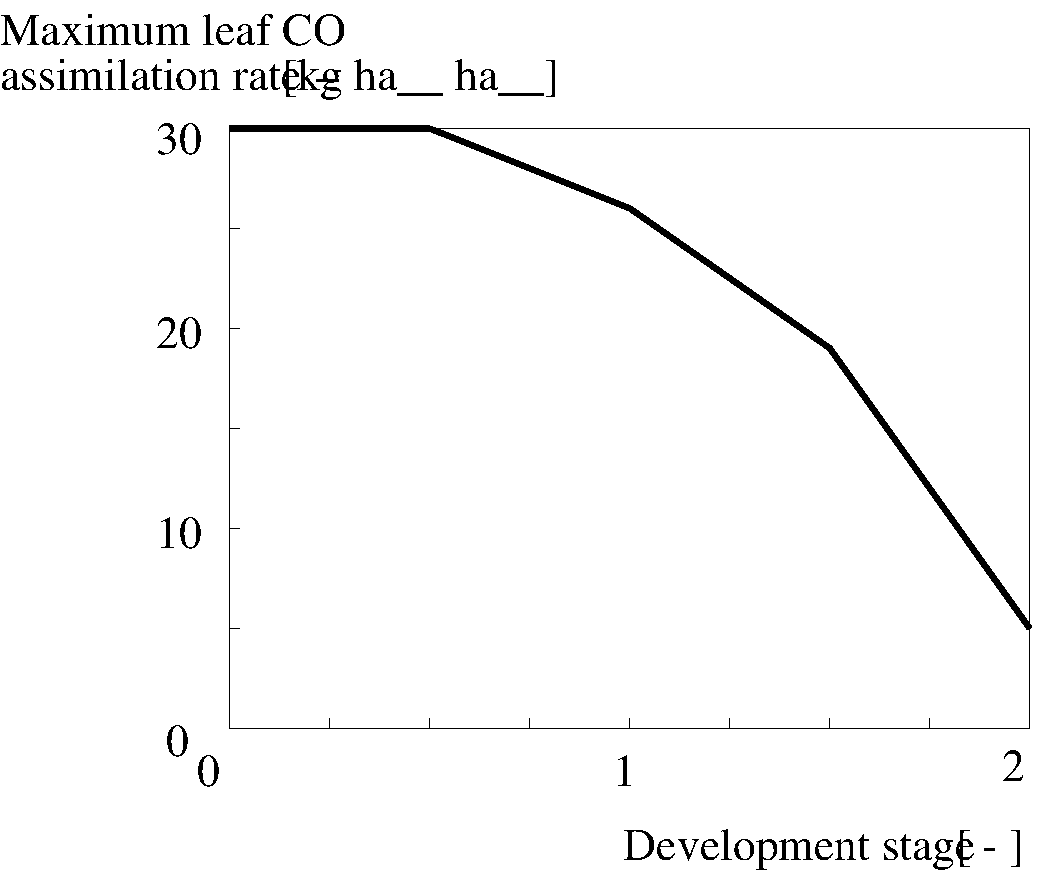
\includegraphics[width=85mm]{\FigDir/AMAXTB.pdf}
	\caption{Maximum leaf CO$_{{\rm 2}}$ assimilation the rate as a function of development of
		the development stage.}
	\label{fig:AMAXTB}
\end{figure}

\subsubsection{Daytime temperature}
The maximum leaf CO$_{{\rm 2}}$ assimilation rate, A$_{{\rm m}}$, has to be corrected for sub-optimal average
daytime temperatures. The correction factor is determined by the average daytime
temperature and is also crop specific. An AFGEN table (acronym: {\bf TMPFTB}) with the
average day time temperature (\ref{eq:daytimetemp}) as the independent variable is used to describe this
dependency (see also Appendix 2). For an example see figure \ref{fig:TMPFTB}. 
The correction factor has to be multiplied with A$_{{\rm m}}$. 

\begin{figure}[p]
	%figure 5.4
	\centering
	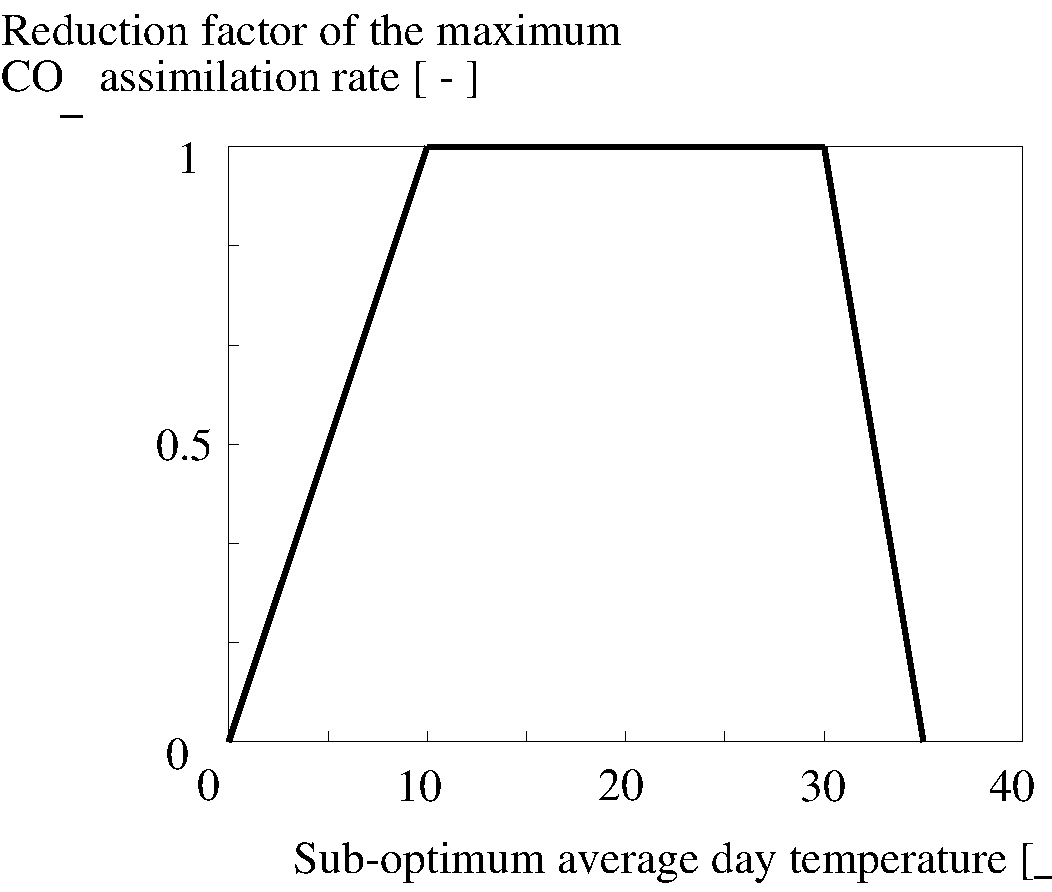
\includegraphics[width=140mm]{\FigDir/TMPFTB.pdf}
	\caption{Reduction factor of the maximum leaf CO$_{{\rm 2}}$ assimilation as a function of
		average temperature.}
	\label{fig:TMPFTB}
\end{figure}

\subsubsection{Nighttime temperature}
The gross CO$_{{\rm 2}}$ assimilation rate cannot exceed the maximum CO$_{{\rm 2}}$ assimilation rate. It
should also be noted that assimilation is an enzymatic process and such processes are
temperature dependent (Downes, 1970). However, there seems to be a considerable
adaption of the assimilation processes to fluctuating and varying temperatures (de Wit {\it et
	al.}, 1978). A wide temperature range for optimum photosynthetic performance under field
conditions is observed (Wardlaw, 1974). Low nighttime temperatures also affect the
assimilation. At night the assimilates, produced during daytime, are transformed into
structural biomass. This process is hampered by low temperature. If these low temperatures prevail 
for a several days, the assimilates accumulate in the plant and the assimilation rate diminishes 
and ultimately halts.

In the model, this temperature effect is accounted for by introducing a correction factor,
which should be multiplied with A$_{{\rm m}}$. This correction factor is a function of low minimum
temperature and is crop specific. An AFGEN table (acronym: {\bf TMNFTB}) is used to
describe this dependency.

As a measure for quantifying the effect of low minimum temperature, the seven day
running average of minimum temperature is used as the independent variable in the
AFGEN table (see also Appendix 2).

\begin{equation}
% eq 5.33
T _{low} ~=~\begin{array}{c}{i=7}  \\
\sum  \\
{i=1}\end{array}{\frac{\, T _{\min ,i} }{7}}
\end{equation}

Where:\\[5pt]
\begin{tabularx}{\textwidth}{llXr}
	T$_{{\rm min}}$  &:& Daily minimum temperature   &     [\degrees C]\\
	T$_{{\rm low}}$ &:& Seven day running average of minimum temperature    &    [\degrees C]\\
	i &:& Day    &    [-]
\end{tabularx}


\subsubsection{Photosynthesis in terms of CH$_{{\rm 2}}$O}
In the photosynthesis process, CO$_{{\rm 2}}$ is reduced to carbohydrates (CH$_{{\rm 2}}$O) using the energy
supplied by the absorbed light. The overall chemical reaction of this complex process is:

\begin{equation}
% equation 5.34
6\, CO_{2} ~+~ 6\, H_{2}O ~~ \underrightarrow{light} ~~ C_{6} H_{12} O_{6} ~+~ 6\, O_{2}
\end{equation}

or in simplified form:

\begin{equation}
% equation 5.35
CO_{2} ~+~ H_{2} O~~ \underrightarrow{light} ~~ CH_{2} O ~+~ O_{2}
\end{equation}

For each kg of CO$_{{\rm 2}}$ absorbed, 30/44 kg of CH$_{{\rm 2}}$O is formed, the numerical values
representing the molecular weights of CH$_{{\rm 2}}$O and CO$_{{\rm 2}}$ respectively.

\begin{equation}
% equation 5.36
R _{d}^{1} ~=~ A _{d}^{1} \,\,{\frac{30}{44}}
\end{equation}

Where:\\[5pt]
\begin{tabularx}{\textwidth}{llXr}
	R$^{{\rm 1}}$$_{{\rm d}}$ &:& Gross daily CH$_{{\rm 2}}$O assimilation rate 
	(not corrected for water stress) &   [kg ha$^{{\rm -1}}$ d$^{{\rm -1}}$]\\
	A$^{{\rm 1}}$$_{{\rm d}}$ &:& Gross daily CO$_{{\rm 2}}$ assimilation rate 
	(see eq. \ref{eq:5.11}) (corrected for low minimum temperature)   &    [kg ha$^{{\rm -1}}$ d$^{{\rm -1}}$]\\   
\end{tabularx}

As mentioned earlier, the gross daily CO$_{{\rm 2}}$ assimilation rate, A$^{{\rm 1}}$$_{{\rm d}}$, 
can be calculated by multiplying the total hourly instantaneous assimilation rate (eq. \ref{eq:5.31}) 
with the day length (eq. \ref{eq:AstroDaylength}). 


%\subsection{Reductions for water, oxygen and nutrient stress}
%\label{sec:PhotosynthesisReductionFactors}

\subsubsection{Water stress}
The calculated daily assimilation in CH$_{{\rm 2}}$O per ha will be reduced when crop transpiration
is reduced. The latter is caused by reduced water update by roots either due to water shortage or water 
surplus causing oxygen stress. In the model the effects of water stress on assimilation are related 
to the ratio of actual transpiration and potential transpiration (van Keulen \& Seligman, 1987).
The reduction factor for transpiration reduction can thus be calculated as.

\begin{equation}
\label{eq:5.37}
RF_{tra} ~=~ {\frac{T _{a} }{T _{p} }}
\end{equation}

Where:\\[5pt]
\begin{tabularx}{\textwidth}{llXr}
	$RF_{{\rm tra}}$ &:& Reduction factor for reduced transpiration rates   & [-]\\
	T$_{{\rm a}}$ &:& Actual transpiration   &     [cm d$^{{\rm -1}}$]\\
	T$_{{\rm p}}$ &:& Potential transpiration   &     [cm d$^{{\rm -1}}$]\\
\end{tabularx}

In \S \ref{sec:evapotranspiration} the calculation of the potential, T$_{{\rm p}}$, and actual 
the transpiration, T$_{{\rm a}}$, will be explained.

\subsubsection{Nutrient stress}

Stress factors are calculated based on the mass concentrations of N/P/K in
the leaf and stem biomass of the plant. For each pool of nutrients, four
concentrations are calculated based on the biomass for leaves and stems:
\begin{itemize}
	\item the actual concentration $C_{a}$ based on the actual amount of nutrients
	divided by the actual leaf and stem biomass.
	\item The maximum concentration $C_{m}$, being the maximum that the plant can absorb
	into its leaves and stems.
	\item The critical concentration $C_{c}$, being the concentration that is needed to
	maintain growth rates that are not limited by N/P/K. For P and K, the
	critical concentration is usually equal to the maximum concentration.
	For N, the critical concentration can be lower than the maximum
	concentration. This concentration is sometimes called 'optimal
	concentration'.
	\item The residual concentration $C_{r}$ which is the amount that is locked
	into the plant structural biomass and cannot be mobilized anymore.
\end{itemize}

The stress index for each nutrient is determined as a simple ratio between those 
concentrations according to:

\begin{equation}
SI = \frac{C_{a} - C_{r}}{C_{c} - C_{r}}
\end{equation}

This equation is applied in analogue to N, P and K and results in the
nitrogen nutrition index ($NNI$), phosphorous nutrition index ($PNI$) and
Potassium nutrition index ($KNI$). Next, the NPK index ($NPKI$) is calculated
as the minimum of $NNI$, $PNI$, $KNI$. 

\begin{equation}
NPKI = min(NNI, KNI, PNI)
\end{equation}

Finally, the reduction factor for
assimilation ($RF_{NPK}$) is calculated using the response parameter for nutrient
shortage on light use efficiency ($NLUE_{NPK}$).

\begin{equation}
RF_{NPK} = 1 - NLUE_{NPK}(1 - NPKI)^{2} ~~~~~~~~~0~\le ~RF_{NPK} ~\le ~1
\end{equation}


\begin{figure}[p]
	\centering
	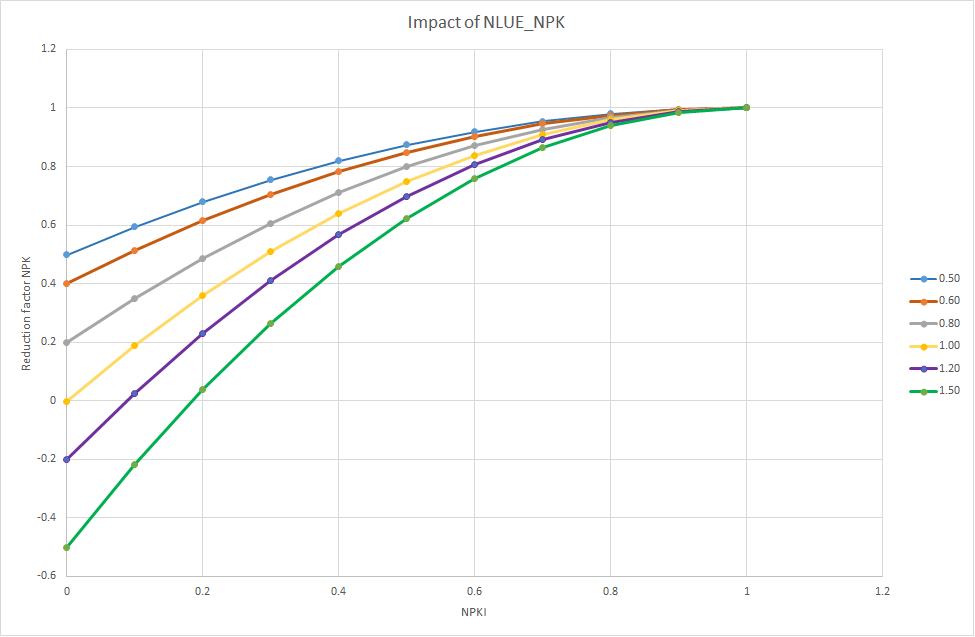
\includegraphics[width=140mm]{\FigDir/Impact_NLUE_NPK.png}
	\caption{Reduction factor of the gross photosynthesis rate as a function of
		$NPKI$ and for different values of $NLUE_{NPK}$.}
	\label{fig:NLUE_NPK}
\end{figure}


\subsubsection{Combined transpiration and nutrient stress}

In situations where both transpiration and nutrients are limiting the daily assimilation rate,
the model will select the minimum value of the reduction factors $RF_{TRA}$ and $RF_{NPK}$. This
reduction factor is multiplied by the assimilation rate in order to compute the actual gross
assimilation rate.


\section{Maintenance respiration}

Some of the carbohydrates formed are respired to provide energy for maintaining the
existing biostructures. The maintenance processes include resynthesis of degraded proteins
(especially enzymes) and maintenance of ionic gradients across cell membranes. The
higher the metabolic activity of the plant, the higher the maintenance costs (Penning de
Vries, 1975), probably due to a higher enzyme turnover and higher transport costs.

Maintenance respiration provides the energy for living organisms to maintain their
biochemical and physiological status. Through the reaction which is the reverse of CO$_{{\rm 2}}$
reduction in the CO$_{{\rm 2}}$ assimilation, the radiation energy which was fixed in the
photosynthetic process is released in a suitable form (ATP and NADPH):

\begin{equation}
% eq 5.38
CH _{2} O ~+~ O _{2} ~\longrightarrow~ CO _{2} ~+~ H _{2} O ~+~ energy
\end{equation}

This maintenance respiration consumes roughly 15 - 30\% of the carbohydrates produced
by a crop in a growing season (Penning de Vries {\it et al.}, 1979). This indicates the
importance of accurate quantification of this process in the model.

\subsection{Maintenance respiration as a function of the weight of dry matter}
The maintenance costs may be estimated on the basis of the quantities of proteins and
minerals present in the biomass and on crop metabolic activity, as presented by De Wit {\it et
	al.} (1978). This method, however, requires information on the nitrogen and mineral
contents of the vegetation.
Based on the results of this analysis, typical values for the maintenance coefficients of
various plant organs have been derived by Penning de Vries \& van Laar (1982).
In the model, these coefficients are used to calculate the maintenance requirements of the
crop. According to this approach the maintenance requirements are approximately 
proportional to the dry weights of the plant organs to be maintained: 

\begin{equation}
\label{eq:5.39}
R _{m,r} ~ = ~\begin{array}{c} {i=1}  \\
\sum  \\
{i=4}\end{array} \, c _{m,i} \, W _{i}
\end{equation}

Where:\\[5pt]
\begin{tabularx}{\textwidth}{llXr}
	R$_{{\rm m,r}}$ &:& Maintenance respiration rate at reference 
	temperature of 25 \degrees C &   [kg ha$^{{\rm -1}}$ d$^{{\rm -1}}$]\\
	c$_{{\rm m,i}}$ &:& Maintenance coefficient of organ i  & [kg kg$^{{\rm -1}}$ d$^{{\rm -1}}$]\\
	W$_{{\rm i}}$ &:& Dry matter weight organ i (see eq. \ref{eq:5.49})   &     [kg ha$^{{\rm -1}}$]\\
	i &:& Leaves (lv), storage organs (so), stems (st) or roots (rt)\\ 
\end{tabularx}

The maintenance coefficient of organ i, {\bf c$_{{\rm m,i}}$}, is crop dependent and should be provided by
the user. Acronyms used in the model: {\bf RML} (lv), {\bf RMO} (so), {\bf RMS} (st) and {\bf RMR} (rt).

In \S \ref{sec:DMpartitioning}, $\Delta$W$_{{\rm i}}$, the increase of the dry matter weight of 
organ i per time step, will be
discussed. Integration of $\Delta$W$_{{\rm i}}$ over the previous time steps yields the total dry matter
weight of organ i (dead and alive). Integration of the net increase of dry matter, $\Delta$Wn$_{{\rm i}}$,
(see eq. \ref{eq:5.48}) over the previous time steps yields the living dry matter weight of organ i
(see eq \ref{eq:5.49}).

\subsection{Dependency of the maintenance respiration on development stage}
The calculated maintenance respiration rate (eq. \ref{eq:5.39}) has to be corrected for senescence.
This correction factor is crop specific and is defined as a function of development stage
(see figure 5.5). An AFGEN table (acronym: {\bf RFSETB}) with the development stage as
independent variable, is used to describe this dependency. The maintenance respiration
should be multiplied with this factor.  Note that differences in nitrogen contents in the different organs 
due to aging of the plant may cause differences in the maintenance coefficients. Although the 
N content per plant organ is simulated by WOFOST8, there is no impact on the maintenance respiration.

\begin{figure}[htbp]
	%figure 5.5
	\centering
	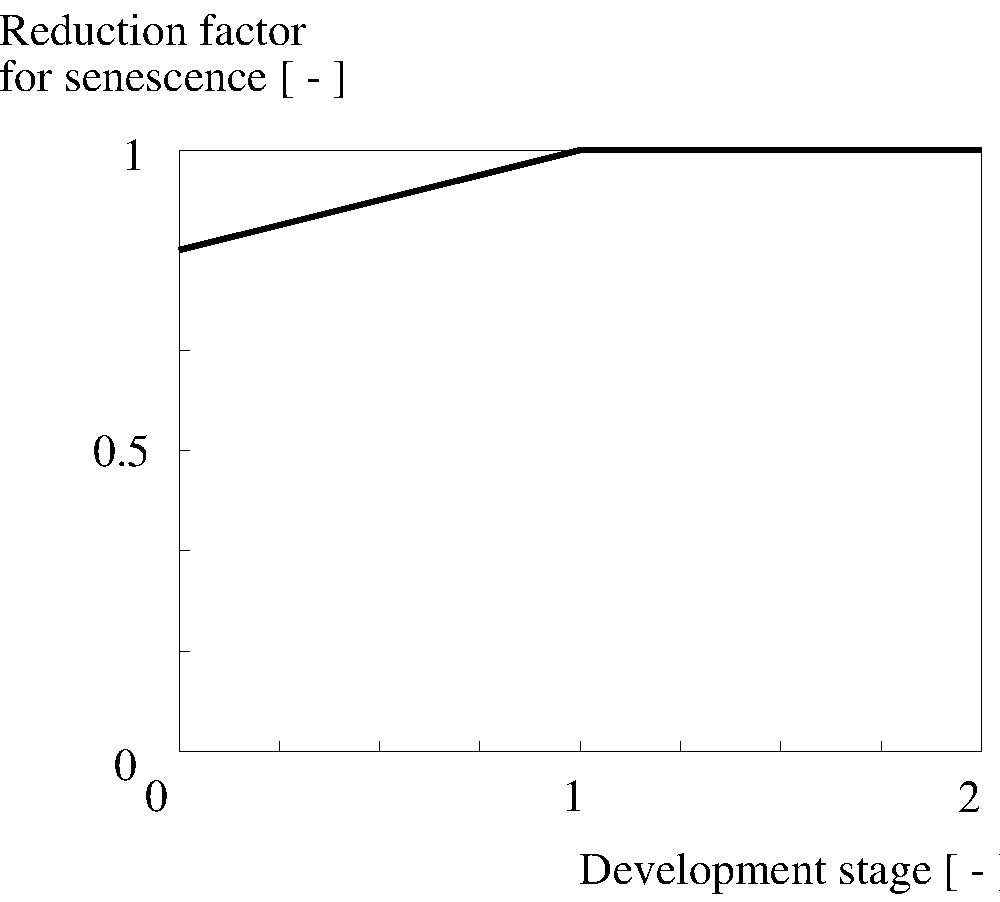
\includegraphics[width=85mm]{\FigDir/RFSETB.pdf}
	\caption{Reduction factor for senescence as a function of development stage}
	\label{fig:RFSETB}
\end{figure}

\subsection{Dependency of the maintenance respiration on temperature}
Higher temperatures accelerate the turnover rates in plant tissue and hence the costs of
maintenance. An increase in temperature of 10\degrees C increases maintenance respiration by a
factor of about 2 (Kase \& Catsky, 1984; Penning de Vries \& van Laar, 1982). However,
in order to be more flexible, in the model a variable {\bf Q$_{{\rm 10}}$} (acronym: {\bf Q10}) is introduced.
Q$_{{\rm 10}}$ is defined as the relative increase of the respiration rate per 10\degrees C temperature
increase. Q$_{{\rm 10}}$ should be provided by the user. The rate of the maintenance respiration at a
certain temperature, can be calculated with:

\begin{equation}
\label{eq:5.40}
R _{m,T} ~=~ R _{m,r} \, Q _{10}^{~~{\frac{T-T _{r} }{10}} }
\end{equation}

Where:\\[5pt]
\begin{tabularx}{\textwidth}{llXr}
	R$_{{\rm m,T}}$ &:& Maintenance respiration rate at 
	temperature T &    [kg ha$^{{\rm -1}}$ d$^{{\rm -1}}$]\\
	R$_{{\rm m,r}}$ &:& Maintenance respiration rate at reference 
	temperature of 25 \degrees C (see eq. \ref{eq:5.39})   &     [kg ha$^{{\rm -1}}$ d$^{{\rm -1}}$]\\
	Q$_{{\rm 10}}$ &:& Relative increase of the respiration rate
	per 10\degrees C temperature increase    &    [-]\\
	T &:& Average daily temperature    &     [\degrees C]\\
	T$_{{\rm r}}$ &:& Reference temperature {\small [=25 \degrees C in 
		the model]}    &    [\degrees C]\\
\end{tabularx}


For tropical species, the reference temperature may be 10\degrees C higher than for species from
temperate climates. The maintenance requirements of a crop are likely to be adapted to
the higher growth temperatures. However, in WOFOST 8.0 the reference temperature is
fixed at 25\degrees C for all crops.

As stated before, maintenance respiration rate depends on the amount of dry matter in the
various organs, the relative maintenance rate per organ and the temperature. It cannot
exceed the actual gross assimilation rate. It is assumed that the vegetation will not be
'self-consuming' in terms of carbohydrates. Actual gross assimilation rate minus 
maintenance respiration rate results in the amount of assimilates available for conversion into
structural material. When the crop ages, its metabolic activity and therefore its
maintenance requirements decreases. This effect could be accounted for by relating 
the maintenance coefficients to the N content of the tissues (van Keulen \& Seligman, 1987).


\section{Transpiration and evaporation}
\label{sec:evapotranspiration}

Transpiration, or the rate of water loss from the plants depends on the energy available
for vaporization, on the difference in vapor pressure between the plant and the surrounding 
air and on the resistance to water vapor diffusion from the stomatal cavity to the
atmosphere (van Keulen \& Seligman, 1987). Potential transpiration is the water loss from
a field crop which covers the soil completely and has an optimum supply of water from
the soil. 

\subsection{Evaporation and transpiration}
Potential evapotranspiration of a crop ET0 is the sum of potential transpiration T$_{{\rm m}}$ and
soil evaporation E0$_{{\rm s}}$.

\begin{equation}
\label{eq:6.2}
ET0 ~=~ E0_{s} ~+~ T_{m} 
\end{equation}

Where:\\[5pt]
\begin{tabularx}{\textwidth}{llXr}
	ET0 &:& Potential evapotranspiration rate (see \S 4.1.3) & [cm d$^{{\rm -1}}$]\\
	E0$_{{\rm s}}$ &:& Potential evaporation of a bare soil (see \S 4.1.3)  & [cm d$^{{\rm -1}}$]\\
	T$_{{\rm m}}$ &:& Maximum crop transpiration rate (see eq. 6.4)  & [cm d$^{{\rm -1}}$]\\
\end{tabularx}

For some crops the potential evapotranspiration can be higher than the Penman-Monteith
reference evapotranspiration. 
Therefore, in the model a correction factor, a so called  crop coefficient
(acronym: {\bf CFET}) is introduced to account for this effect. The Penman-Monteith evapotranspiration
should be multiplied by this crop coefficient (Feddes, 1978; Doorenbos \& Pruitt, 1977).
The evaporation is reduced due to the presence of vegetation, which intercepts the solar
energy and reduces the windspeed. The evaporation of the soil as a function of the leaf
area index (Goudriaan, 1977; Ritchie, 1972; 1971) can be estimated as:

\begin{equation}
\label{eq:6.3}
E0 _{s} ~=~ ET0 \cdot e^{-\kappa_{gb} \cdot LAI}
\end{equation}

Where:\\[5pt]
\begin{tabularx}{\textwidth}{llXr}
	E0$_{{\rm s}}$ &:& Potential bare soil evaporation  & [cm d$^{{\rm -1}}$]\\
	$\kappa$$_{{\rm gb}}$ &:& Extinction coefficient for global radiation  & [-]\\
	LAI &:& Leaf area index  & [ha ha$^{{\rm -1}}$]\\
\end{tabularx}

The potential transpiration rate can be calculated by combining equations \ref{eq:6.2} and 
\ref{eq:6.3}.

\begin{equation}
\label{eq:6.4}
T _{m} ~=~ ET0\, (1~-~e ^{-\kappa _{gb} \, LAI} )
\end{equation}

Where:\\[5pt]
\begin{tabularx}{\textwidth}{llXr}
	T$_{{\rm m}}$ &:& Maximum crop transpiration rate & [cm d$^{{\rm -1}}$]\\
	ET0 &:& Potential evapotranspiration rate & [cm d$^{{\rm -1}}$]\\
	$\kappa$$_{{\rm gb}}$ &:& Extinction coefficient for global radiation & [-]\\
	LAI &:& Leaf area index (see \S \ref{sec:5.4.5}) & [ha ha$^{{\rm -1}}$]\\
\end{tabularx}

The extinction coefficient for global radiation can be estimated as a factor times the
extinction coefficient of diffuse radiation:

\begin{equation}
\label{eq:6.5}
\kappa_{gb} ~=~ 0.75\, \kappa_{df} 
\end{equation}

Where:\\[5pt]
\begin{tabularx}{\textwidth}{llXr}
	$\kappa_{{\rm gb}}$ &:& Extinction coefficient for global radiation & [-]\\
	$\kappa_{{\rm df}}$ &:& Extinction coefficient for diffuse light & [-]\\
\end{tabularx}

The maximum evaporation rate from a shaded water surface can be calculated in the same
way as equation \ref{eq:6.4}: 

\begin{equation}
\label{eq:6.6}
E_{w,\max } ~=~ E0_{w} \cdot e^{-\kappa_{gb} LAI}
\end{equation}

Where:\\[5pt]
\begin{tabularx}{\textwidth}{llXr}
	E$_{{\rm w,max}}$ &:& Maximum evaporation rate from a shaded water surface & 
	[cm d$^{{\rm -1}}$]\\
	E0$_{{\rm w}}$ &:& Potential evaporation rate from a water surface 
	(see \S \ref{sec:penman}) & [cm d$^{{\rm -1}}$]\\
	$\kappa$$_{{\rm gb}}$ &:& Extinction coefficient for global radiation & [-]\\
	LAI &:& Leaf area index & [ha ha$^{{\rm -1}}$]\\
\end{tabularx}

The maximum evaporation rate from a shaded bare soil surface can also be calculated in
the same way as in equation \ref{eq:6.4} and \ref{eq:6.6}:

\begin{equation}
\label{eq:6.7}
E_{s,\max } ~=~ E0 _{s} \,\,\, e ^{-\kappa  _{gb} LAI}
\end{equation}

Where:\\[5pt]
\begin{tabularx}{\textwidth}{llXr}
	E$_{{\rm s,max}}$ &:& Maximum evaporation rate from a shaded 
	soil surface & [cm d$^{{\rm -1}}$]\\
	E0$_{{\rm s}}$ &:& Potential evaporation rate from a bare soil 
	surface & [cm d$^{{\rm -1}}$]\\
	$\kappa$$_{{\rm gb}}$ &:& Extinction coefficient for total global radiation & [-]\\
	LAI &:& Leaf area index & [ha ha$^{{\rm -1}}$]\\
\end{tabularx}

\subsection{Reduction of the transpiration due to water stress}

For the potential yield level the actual transpiration rate is always equal to the maximum
transpiration rate, because sufficient water is available. The actual transpiration rate is
calculated from the maximum transpiration rate, taking into account reductions for
shortage or excess of water in the root zone. Water uptake by the roots depends on the
difference in potential between the water in the plant and in the soil, and on the resistance
to transport of moisture from the soil to the atmosphere (van Keulen \& Seligman, 1987).
In contrast to Feddes {\it et al}. (1978) not soil water potential, but soil water content is
chosen as the independent variable (Gollan {\it et al}., 1986; Schulze 1986).

Up to a point, the water potential in the plant can be adapted in order to maintain
potential transpiration. At what soil moisture content the transition from potential
transpiration to a transpiration deficit takes place, is difficult to quantify. In the model,
the actual transpiration for the water limited run is obtained by multiplying the potential
transpiration with a reduction factor. This reduction factor is defined as (van Diepen {\it et al}., 1988):

\begin{equation}
\label{eq:6.8}
R_{ws} ~=~{\frac{\theta_{t} ~-~ \theta  _{wp} }{ \ _{ws} ~-~ \theta_{wp} }}
\end{equation}

Where:\\[5pt]
\begin{tabularx}{\textwidth}{llXr}
	$R_{{\rm ws}}$ &:& Reduction factor for transpiration in case of
	water shortage & [-]\\
	$\theta_{{\rm t}}$ &:& Actual soil moisture content (see eq. 6.1 and 
	6.34) & [cm$^{{\rm 3}}$ cm$^{{\rm -3}}$]\\
	$\theta_{{\rm wp}}$ &:& Soil moisture content at wilting 
	point & [cm$^{{\rm 3}}$ cm$^{{\rm -3}}$]\\
	$\theta_{{\rm ws}}$ &:& Critical soil moisture & [cm$^{{\rm 3}}$ cm$^{{\rm -3}}$]\\ 
\end{tabularx}

The critical soil moisture content is defined as the quantity of stored soil moisture below
which water uptake is impaired and the crop begins to close its stomata. It is not a fixed
value. Restriction of water uptake due to water stress starts at a higher water content
when the potential transpiration rate is higher (Denmead \& Shaw, 1962). The critical
moisture content can be calculated as (van Diepen {\it et al}., 1988):

\begin{equation}
\label{eq:6.9}
\theta_{ws} ~=~ (1\, -\, p )\, (\theta_{fc} \, -\, \theta_{wp} )\, +\, \theta_{wp} 
\end{equation}

Where:\\[5pt]
\begin{tabularx}{\textwidth}{llXr}
	$\theta$$_{{\rm ws}}$ &:& Critical soil moisture content & [cm$^{{\rm 3}}$ cm$^{{\rm -3}}$]\\
	p &:& Soil water depletion fraction as a function 
	of pot. evapotranspiration & [cm$^{{\rm 3}}$ cm$^{{\rm -3}}$]\\
	$\theta$$_{{\rm fc}}$ &:& Soil moisture content at field capacity & [cm$^{{\rm 3}}$ cm$^{{\rm -3}}$]\\
	$\theta$$_{{\rm wp}}$ &:& Soil moisture content at wilting point & [cm$^{{\rm 3}}$ cm$^{{\rm -3}}$]\\
\end{tabularx}

The soil moisture content at field capacity, {\bf $\theta$$_{{\rm fc}}$} (acronym: {\bf SMFCF}), 
and the soil moisture content at wilting point, {\bf $\theta$$_{{\rm wp}}$} (acronym: {\bf SMW}), 
are soil specific and should be given by the user. The soil water depletion fraction, p, is 
a function of the potential evapotranspiration rate (for a closed canopy) and the crop group 
number. It is established in subroutine
{\bf SWEAF}. In literature, instead of the term soil water depletion fraction, also the 
expression easily available water is used. Easily available water is defined as the amount of
water between $\theta$$_{{\rm fc}}$ and $\theta$$_{{\rm wp}}$ which can be extracted from the root 
zone without reducing the
transpiration. Indicative p-values for the most important crops at different values of ET0
are presented in Table 6.1. The crop group number ranges from 1 (drought-sensitive) to 5
(drought-resistant). An example of a classification of the different crop groups is
presented in Table 6.2.

\begin{table}
	% Table 6.1
	\caption{Soil water depletion fraction (p) as a function of potential evapotranspiration 
		of a closed crop canopy for different crop groups (Doorenbos {\it et al}.,1978).}
	\label{tbl:soilwatdeplfraction}
	\begin{tabularx}{\textwidth}{Xrrrrrrrrr}
		\hline
		\multicolumn{10}{c}{Crop ET0 in cm d-1}\\
		\hline
		group$^{\rm *}$ & 0.2 & 0.3 & 0.4 & 0.5 & 0.6 & 0.7 & 0.8 & 0.9 & 1.0\\
		1 & 0.45 & 0.38 & 0.30 & 0.25 & 0.23 & 0.20 & 0.18 & 0.16 & 0.15\\
		2 & 0.60 & 0.50 & 0.43 & 0.35 & 0.30 & 0.28 & 0.25 & 0.23 & 0.20\\
		3 & 0.75 & 0.65 & 0.55 & 0.45 & 0.40 & 0.38 & 0.33 & 0.30 & 0.25\\
		4 & 0.85 & 0.75 & 0.65 & 0.55 & 0.50 & 0.48 & 0.43 & 0.38 & 0.35\\
		5 & 0.92 & 0.85 & 0.75 & 0.65 & 0.60 & 0.55 & 0.50 & 0.48 & 0.45\\
		\hline 
	\end{tabularx} 
\end{table}


\begin{table}
	% Table 6.2
	\caption{Example of crops in the different crop groups (Doorenbos {\it et al}., 1978).}
	\label{tbl:ExampleCropGroups}
	\begin{tabularx}{\textwidth}{lX}
		\hline
		Group no & Representative crop types\\
		\hline
		1 & leaf vegetables, strawberry\\     
		1-2 & cabbage, onion\\
		2 & clover, carrot, early tobacco\\     
		2-3 & banana, pepper\\
		3 & grape, pea, potato\\
		3-4 & bean, sunflower, tomato, water melon, grass\\
		4 & citrus, groundnut, pineapple\\
		4-5 & alfalfa cotton, tobacco, cassava, sweet potato, grains\\
		5 & olive, safflower, sorghum, soybean, sugarcane\\
		\hline
	\end{tabularx}
\end{table}

The soil water depletion fraction for very high values of potential evapotranspiration of a
closed canopy can be as low as 0.10. For very low values of potential evapotranspiration
of a closed canopy this fraction can be as high as 0.96.
Note that it is possible that the reduction factor R$_{{\rm ws}}$ (eq. \ref{eq:6.8}) might obtain 
values higher
than unity and lower than zero for certain values of p and $\theta$$_{{\rm t}}$. Since this does not make
any sense, in the model the highest possible value for R$_{{\rm ws}}$ is set to unity and the lowest
possible value is set to zero.
An empirical formula can be used to calculate the fraction of easily available soil water,
yielding identical values as the ones given in the Table \ref{tbl:soilwatdeplfraction} 
(van Diepen {\it et al}., 1988).

\begin{equation}
\label{eq:6.10}
p~={\frac{~1}{ \alpha _{p} ~+~ \beta _{p} ~ET0}} ~-~ 0.10\, (\, 5~-~No _{cg} \, )
\end{equation}

Where:\\[5pt]
\begin{tabularx}{\textwidth}{llXr}
	p &:& Fraction of easily available soil water  & [cm$^{{\rm 3}}$ cm$^{{\rm -3}}$]\\
	$\alpha$$_{{\rm p}}$ &:& Regression constant {\small (=0.76 van Diepen et al., 1988)}  & [-]\\
	$\beta$$_{{\rm p}}$ &:& Regression constant {\small (=1.5 van Diepen et al., 1988)}  & [d cm-$^{{\rm 1}}$]\\
	ET0 &:& Potential evapotranspiration rate  & [cm d$^{{\rm -1}}$]\\
	No$_{{\rm cg}}$ &:& Crop Group number {\small (=1 to 5, Doorenbos et al., 1978)}  & [-]\\
\end{tabularx}

Note that crop group number, {\bf No$_{{\rm cg}}$} (acronym: {\bf DEPNR}) is input in the model and should
be provided by the user.

For crop group 1 and 2 this estimate is not very accurate and an additional correction is
applied to reproduce the table values correctly (van Diepen {\it et al}., 1988):

\begin{equation}
%eq 6.11
p~=~p~+~{\frac{ET0 ~-~ 0.6}{No _{cg} \, (\, No _{cg} ~+~3\, )}}
\end{equation}

Where:\\[5pt]
\begin{tabularx}{\textwidth}{llXr}
	where p &:& Fraction of easily available soil water  & [cm$^{{\rm 3}}$ cm$^{{\rm -3}}$]\\
	ET0 &:& Potential evapotranspiration rate  & [cm d$^{{\rm -1}}$]\\
	No$_{{\rm cg}}$ &:& Crop Group number {\small (=1 to 5, Doorenbos et al., 1978)}  & [-]\\
\end{tabularx}

\subsection{Reduction of the transpiration due to oxygen stress}
The transpiration rate of the plants can also be reduced when the root zone is completely
saturated. Root systems which have been developed in aerobic soils do not have airducts
and degenerate within several days when anaerobic conditions (waterlogging) are imposed
(Penning de Vries {\it et al}., 1989). Flooding quickly depletes the O$_{{\rm 2}}$ in the soil and root cells
disintegrate when their metabolic activities are hampered by oxygen depletion. For
detailed information on the physiological effects of excess water on a crop see Jackson
and Drew (1984).

Reduction in transpiration occurs when the actual soil moisture content exceeds the
critical soil moisture content for aeration. The critical soil moisture content for aeration
can be calculated as:

\begin{equation}
\label{eq:6.12}
\theta_{air} ~=~ \theta_{\max} ~-~\theta_{c} 
\end{equation}

Where:\\[5pt]
\begin{tabularx}{\textwidth}{llXr}
	$\theta$$_{{\rm air}}$ &:& Critical soil moisture content for aeration & [cm$^{{\rm 3}}$ cm$^{{\rm -3}}$]\\
	$\theta$$_{{\rm max}}$ &:& Soil porosity & [cm$^{{\rm 3}}$ cm$^{{\rm -3}}$]\\
	$\theta$$_{{\rm c}}$ &:& Critical air content & [cm$^{{\rm 3}}$ cm$^{{\rm -3}}$]\\
\end{tabularx}

The soil porosity, {\bf $\theta$$_{{\rm max}}$} (acronym: {\bf SMO}) and the critical soil air 
content, {\bf $\theta$$_{{\rm c}}$} (acronym:{\bf CRAIRC}), are soil specific and should 
be provided by the user. 

In the model, maximum reduction is reached after four successive days of anaerobic
conditions. In reality however, this period depends on the development stage and on the
species. If at the fifth successive day oxygen shortage occurs the reduction remains the
same as on the fourth day. The reduction factor for the transpiration rate due to oxygen
shortage can be calculated as (van Diepen, personal communication):

\stepcounter{equation}
\begin{align}
\label{eq:6.13a-b}
R_{os,\max } &= \frac{ \theta  _{\max } ~-~ \theta  _{t} }{\theta _{\max } ~-~ \theta  _{air} } \subeqn  \\
R_{os} &= 1 - \frac{No _{d} }{4} \, (\, 1\, -\, R _{os,\max } \, ) ~~~ with~~ No_{d} ~\le ~ 4 \subeqn
\end{align}

Where:\\[5pt]
\begin{tabularx}{\textwidth}{llXr}
	R$_{{\rm os,max}}$ &:& Maximum reduction factor due to oxygen shortage & [-]\\
	R$_{{\rm os}}$ &:& Reduction factor due to oxygen shortage & [-]\\
	$\theta$$_{{\rm air}}$ &:& Critical soil moisture content for aeration 
	& [cm$^{{\rm 3}}$ cm$^{{\rm -3}}$]\\
	$\theta$$_{{\rm max}}$ &:& Soil porosity & [cm$^{{\rm 3}}$ cm$^{{\rm -3}}$]\\
	$\theta$$_{{\rm t}}$ &:& Actual soil moisture content (see eq. \ref{eq:6.34}) 
	& [cm$^{{\rm 3}}$ cm$^{{\rm -3}}$]\\
	No$_{{\rm d}}$ &:& Number of successive days with oxygen stress & [-]\\
\end{tabularx}

For crops which roots develop airducts, like for example rice, and for crops grown on
perfectly drained land, the reduction factor for oxygen shortage equals unity. If this ratio
is less then unity, the actual transpiration rate is reduced proportionally.

Usually, in freely draining soils oxygen stress does not play any role. It may occur when
the critical soil moisture content for aeration is greater than the soil moisture content at
field capacity and when the subsoil is very slowly permeable. In case of groundwater
influence, oxygen shortage may occur regularly. However, the process of transpiration
reduction due oxygen shortage is poorly parametrized and therefore values for the
reduction factor are rather speculative. 

\subsection{Actual transpiration}
As a result of water excess and/or water shortage the reduction factor for the transpiration rate can be
calculated as:

\begin{equation}
\label{eq:6.14}
RF_{tra} = R_{ws} \,\, R_{os}
\end{equation}

Figure \ref{fig:TaTp_vs_soilmoisture} provides an overview of the ratio $\frac{T_a}{T_p}$ as
a function of soil moisture level $\theta$. 


\begin{figure}[p]
	\centering
	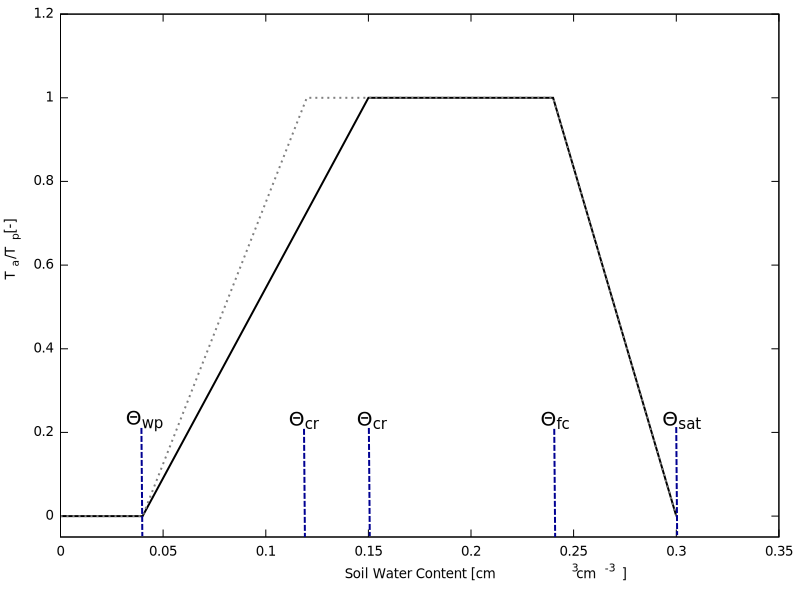
\includegraphics[width=120mm]{\FigDir/figure7.pdf}
	\caption{The relation between soil water content, $\theta$, and Ta/Tp for a crop/soil combination. 
		$\theta_{{\rm wp}}$, $\theta_{cr}$, $\theta_{{\rm wp}}$ and $\theta_{{\rm sat}}$ represent the water
		 content of the soil at wilting point, the critical point for potential transpiration, field capacity 
		 and saturation, respectively. The dashed line represents either a more drought resistant species under
		 the same field conditions, or the same species under a lower evaporative demand, caused by different
		 weather conditions (Penning de Vries et al., 1989; van Laar et al., 1992)}
	\label{fig:TaTp_vs_soilmoisture}
\end{figure}

\section{Nutrients}


\section{Growth}

The amount of the absorbed CH$_{{\rm 2}}$O that remains after correction and reduction of the
gross CO$_{{\rm 2}}$ assimilation rate (e.g. the net assimilation rate) is available to be 
converted into dry matter. Growth, 
in fact is the increase in dry matter ignoring its water content. The net assimilation rate
is thus simply the difference between the gross actual assimilation rate and the losses due to
maintenance respiration:

\begin{equation}
	R_{n} = R_{d} ~-~ R _{m,T} 
\end{equation}

Where:\\[5pt]
\begin{tabularx}{\textwidth}{llXr}
	R$_{{\rm n}}$ &:& Net assimilation rate   &     [kg ha$^{{\rm -1}}$ d$^{{\rm -1}}$]\\
	R$_{{\rm d}}$ &:& Actual daily CH$_{{\rm 2}}$O assimilation rate (see eq. \ref{eq:5.37})   &   
	[kg ha$^{{\rm -1}}$ d$^{{\rm -1}}$]\\
	R$_{{\rm m,T}}$ &:& Maintenance respiration rate at 
	temperature T (see eq. \ref{eq:5.40})   &     [kg ha$^{{\rm -1}}$ d$^{{\rm -1}}$]\\
\end{tabularx}

As it is assumed that the maintenance respiration cannot be larger than the actual gross 
assimilation rate, the net assimilation rate will be zero or larger.

The pattern of dry matter distribution over the various plant organs is closely related to
the development stage of the crop. Development is defined as progression in the successive 
phenological stages. It is characterized by the formation rate of the various vegetative
and reproductive organs and their order of appearance. However, before the growth rates
of the different organs can be computed, first the growth respiration has to be taken into account.

\subsection{Growth respiration}

The conversion of the net assimilate rate into structural plant material requires energy which is
called 'growth respiration' in WOFOST.
In this conversion process of the glucose molecules, CO$_{{\rm 2}}$ and
H$_{{\rm 2}}$O are released. This is a partial combustion of glucose to provide energy required in
the various biochemical pathways. Hence, biosynthesis of the various structural compounds can 
be considered a process of cut and paste, the scraps representing the weight
lost in growth respiration.
Each structural compound is formed along a distinct, non crop-specific pathway.
Following these reactions, the weight of glucose required to produce a unit of the
compound can be calculated (Penning de Vries {\it et al.}, 1974). The transport costs of the
molecules are included. Two active passages of membranes are assumed. Each active
passage requires 1 ATP, which is provided by respiring $^{{\rm 1}}$/$_{{\rm 3}}$$_{{\rm 8}}$ molecule of glucose.

The assimilates required to produce a unit weight of a certain plant organ can now be
calculated from its chemical composition and the assimilate requirements of the various
chemical compounds. Storage organs (grains, tubers, etc.) vary to much in composition
among species for one general value of their assimilate requirements to be given. The
conversion efficiency represents the inverse of the assimilate requirement.

At higher temperatures the conversion processes are accelerated, but the pathways are
identical (Spitters {\it et al.} 1989). Hence, the assimilate requirements do not vary with
temperature. 

As explained, conversion into dry matter costs energy, therefore a conversion factor is
defined. This factor depends on the conversion efficiency of assimilates and on the
partitioning factors of the different organs. The dry matter is multiplied with this overall
conversion efficiency factor to calculate the dry matter increase. The conversion 
efficiency of carbohydrates into structural plant material is calculated as a weighted average
of the efficiencies for the various plant organs.

\begin{equation}
\label{eq:5.42}
C _{e} ~={\frac{~1}{
		\begin{array}{c}
		{i=3}  \\
		\sum  \\
		{i=1}
		\end{array} {pc_{i}}/{C_{e,i}} \cdot (1-pc_{rt} ) + {pc_{rt}}/{C_{e,rt}} 
}}
\end{equation}

Where:\\[5pt]
\begin{tabularx}{\textwidth}{llXr}
	C$_{{\rm e}}$ &:& Conversion efficiency factor of assimilates, total crop  &   
	[kg kg$^{{\rm -1}}$]\\
	C$_{{\rm e,i}}$ &:& Conversion efficiency factor of the assimilates 
	of a specified organ  &      [kg kg$^{{\rm -1}}$]\\
	pc$_{{\rm i}}$ &:& Partitioning factor of organ i   &
	[kg kg$^{{\rm -1}}$]\\
	i &:& Leaves (lv), storage organs (so), stems (st)\\
	rt &:& roots\\
\end{tabularx}

The conversion efficiency factor for the assimilates of a specified organ, {\bf C$_{{\rm e,i}}$}, is crop
specific and should be given by the user. Acronyms used in the model: {\bf CVL} (lv), {\bf CVO}
(so), {\bf CVR} (rt) and {\bf CVS} (st).

The dry matter growth rate of the total crop can be calculated as:

\begin{equation}
% eq 5.43
\Delta W~=~ C_{e} \cdot R_{n} 
\end{equation}

Where:\\[5pt]
\begin{tabularx}{\textwidth}{llXr}
	$\Delta$W &:& Dry matter growth rate total crop   &
	[kg ha$^{{\rm -1}}$ d$^{{\rm -1}}$]\\
	C$_{{\rm e}}$ &:& Conversion efficiency factor of assimilates,
	total crop (see eq. \ref{eq:5.42})    &    [kg kg$^{{\rm -1}}$] \\
	R$_{{\rm n}}$ &:& Net assimilation rate (see \ref{eq:5.41})   &
	[kg ha$^{{\rm -1}}$ d$^{{\rm -1}}$]\\
\end{tabularx}

\subsection{Dry matter partitioning}
\label{sec:DMpartitioning}

In WOFOST the dry matter is partitioned over the 4 parts of the
plant. In the model, total dry matter growth is partitioned according to fixed distribution
factors, defined as a function of development stage. Dry matter is first partitioned
between shoots and roots. 

\stepcounter{equation}
\begin{align}
% eqn 5.44a,b
\Delta W_{rt} &= pc_{rt} \cdot \Delta W   \subeqn  \\
\Delta W_{sh} &= (1 - pc_{rt}) \Delta W \subeqn
\end{align}


Where:\\[5pt]
\begin{tabularx}{\textwidth}{llXr}
	$\Delta$W &:& Dry matter growth rate total crop   &
	[kg ha$^{{\rm -1}}$ d$^{{\rm -1}}$]\\
	$\Delta$W$_{{\rm rt}}$ &:& Dry matter growth rate roots    &
	[kg ha$^{{\rm -1}}$ d$^{{\rm -1}}$]\\
	$\Delta$W$_{{\rm sh}}$ &:& Dry matter growth rate shoots    &
	[kg ha$^{{\rm -1}}$ d$^{{\rm -1}}$]\\
	pc$_{{\rm rt}}$ &:& Partitioning factor of roots    &
	[kg kg$^{{\rm -1}}$]\\
\end{tabularx}

The growth rate of leaves, stems and storage organs is simply the product of the dry
matter growth rate of the shoots and the fraction allocated to these organs.

\begin{equation}
\label{eq:5.45}
\Delta W_{i} ~=~ pc_{i} \cdot \Delta W_{sh} 
\end{equation}

Where:\\[5pt]
\begin{tabularx}{\textwidth}{llXr}
	$\Delta$W$_{{\rm i}}$ &:& Dry matter growth rate of organ i &
	[kg ha$^{{\rm -1}}$ d$^{{\rm -1}}$]\\
	$\Delta$W$_{{\rm sh}}$ &:& Dry matter growth rate of shoots   &
	[kg ha$^{{\rm -1}}$ d$^{{\rm -1}}$]\\
	pc$_{{\rm i}}$ &:& Partitioning factor of organ i    &
	[kg kg$^{{\rm -1}}$]\\
	i &:& Leaves (lv), storage organs (so), stems (st)
\end{tabularx}

The partitioning factors, {\bf pc$_{{\rm i}}$}, are a function of development stage and are crop specific. In
the model, the dependency is described using AFGEN tables with the development stage
as the independent variable (see Appendix 2). Acronyms used in the model: {\bf FLTB} (lv),
{\bf FOTB} (so), {\bf FRTB} (rt) and {\bf FSTB} (st).

At any development stage the following relation must be valid, if not, the simulation will
be stopped (see also fig. 5.6):

\begin{equation}
% eq 5.46
pc_{lv} + pc_{st} + pc_{so} = 1
\end{equation}

Where:\\[5pt]
\begin{tabularx}{\textwidth}{llXr}
	pc$_{{\rm i}}$ &:& Partitioning factor of organ i   &
	[kg kg$^{{\rm -1}}$]\\
	i &:& Leaves (lv), storage organs(so), stems (st)
\end{tabularx}

\begin{figure}[p]
	% fig 5.6
	\centering
	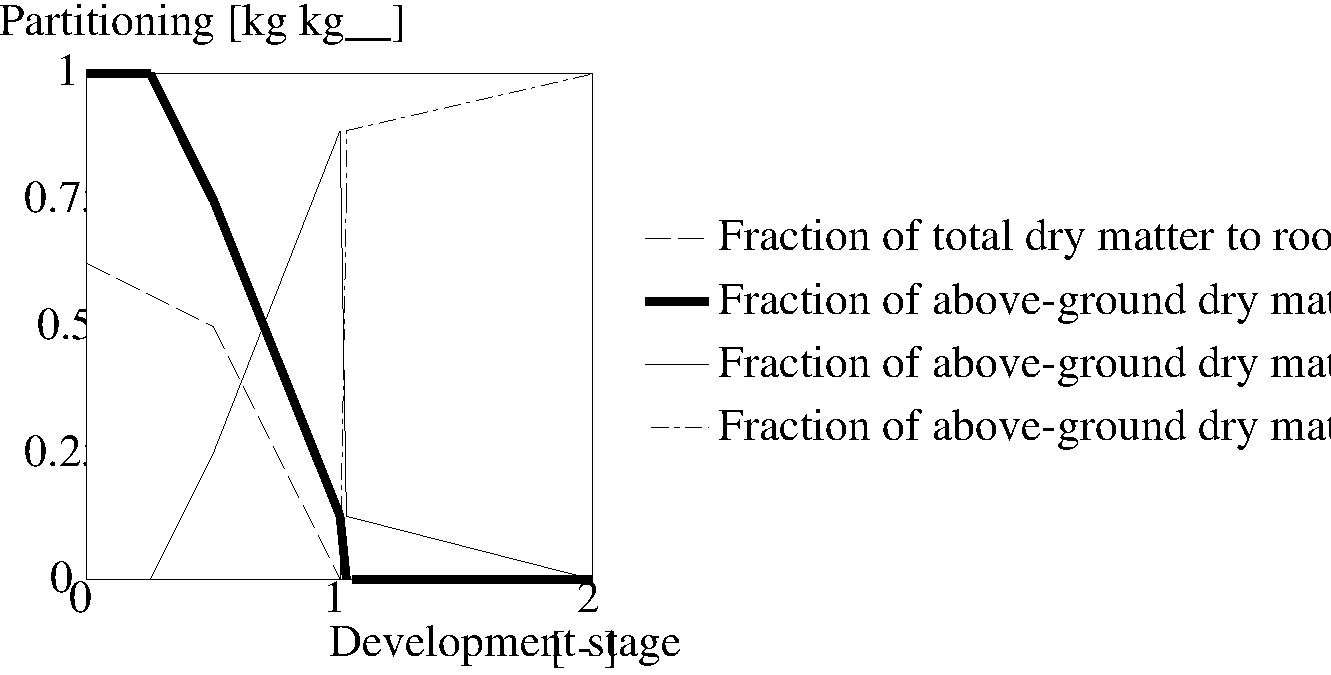
\includegraphics[width=120mm]{\FigDir/FRTB.pdf}
	\caption{Partitioning factors of the different organs as a function of development stage}
	\label{fig:partitioning}
\end{figure}

The actual gross CO$_{{\rm 2}}$ assimilation rate has to be identical to the amount of structural plant
material produced plus the amounts used for maintenance respiration and conversion (see
figure 5.1). The carbon balance has to be zero. 

\begin{equation}
\label{eq:5.47}
0 = {\frac{R_{d} - R_{m,T} - R_{g} \big( pc_{rt} + (pc_{lv} + pc_{st} + pc_{so}) \cdot (1 - pc_{rt}) \big) }{R_d}}  
\end{equation}

Where:\\[5pt]
\begin{tabularx}{\textwidth}{llXr}
	R$_{{\rm g}}$ &:& Growth respiration rate (see eq. \ref{eq:5.41})   &
	[kg ha$^{{\rm -1}}$ d$^{{\rm -1}}$]\\
	R$_{{\rm d}}$ &:& Actual daily CH$_{{\rm 2}}$O assimilation rate (see eq. \ref{eq:5.37})   &
	[kg ha$^{{\rm -1}}$ d$^{{\rm -1}}$]\\
	R$_{{\rm m,T}}$ &:& Maintenance respiration rate (see eq. \ref{eq:5.40})   &
	[kg ha$^{{\rm -1}}$ d$^{{\rm -1}}$]\\
	pc$_{{\rm i}}$ &:& Partitioning factor of organ i    &
	[kg kg$^{{\rm -1}}$]\\
	i &:& Leaves (lv), storage organs (so), stems (st), roots (rt)\\
\end{tabularx}

As mentioned earlier, it is assumed that maintenance respiration can not exceed the actual
gross assimilation rate. However, in case the daily CH$_{{\rm 2}}$O assimilation rate comes close to
zero, this might happen and therefore simulation should be stopped. Introducing a
division by R$_{{\rm d}}$ in the carbon check (eq. \ref{eq:5.47}) will identify the occurrence of such an
event.It should be mentioned that in subsequent versions of the WOFOST model, the carbon
balance check will be simplified.

%\subsection{Growth and leaf senescence  }
%\label{sec:5.4.5}
%
%As is explained in paragraph \ref{sec:DMpartitioning}, the growth rate of a leaves, stems or 
%storage organs is obtained by
%multiplying the growth rate of the shoot by the fraction allocated to that organ.
%Its total dry biomass (dead and alive) is obtained by integrating this growth rate over
%time. Taking the death rate of the different organs into account, the integration of the net
%increase of dry matter, $\Delta$Wn$_{{\rm i}}$, (see eq. \ref{eq:5.48}) over the previous time steps 
%yields the living dry matter weight of organ i (see eq. \ref{eq:5.49}).
%
%This approach of the partitioning of dry matter is descriptive, as the distribution keys are
%defined as a function of the development stage of the crop only. The influence of
%environmental factors could be included by applying modification factors to these keys,
%depending on temperature, water and nutrient status of the crop, and its reserve level
%(Loomis {\it et al.}, 1979; van Keulen \& Seligman, 1987). In the WOFOST model, however,
%this is not applied. Some more attention is paid to the crop growth by introducing a death
%rate for leaves, roots and stems. Death rate is a function of the development stage of the
%plant and is crop and organ specific.

\subsection{Growth of stems, roots and storage organs}

In the model, the death rate of the storage organs is considered to be zero. For the roots
and the stems increase in living biomass can be easily determined as the growth rate
minus death rate. This yields the net growth rate (eq. \ref{eq:5.48}). The death rate is crop
specific and is defined as the daily amount of the living biomass which no longer
participates in the plant processes. The death rate of stems and roots is considered to be a
function of development stage (see fig. \ref{fig:DeathRoots}). This dependency is described using an
AFGEN table with the development stage as the independent variable (see also Appendix
2). The death rate of leaves is more complicated. Leaf senescence due to shading (high
LAI), water stress and also due to exceedance of the life span should be accounted for.


\begin{figure}[p]
	%Fig. 5.7
	\centering
	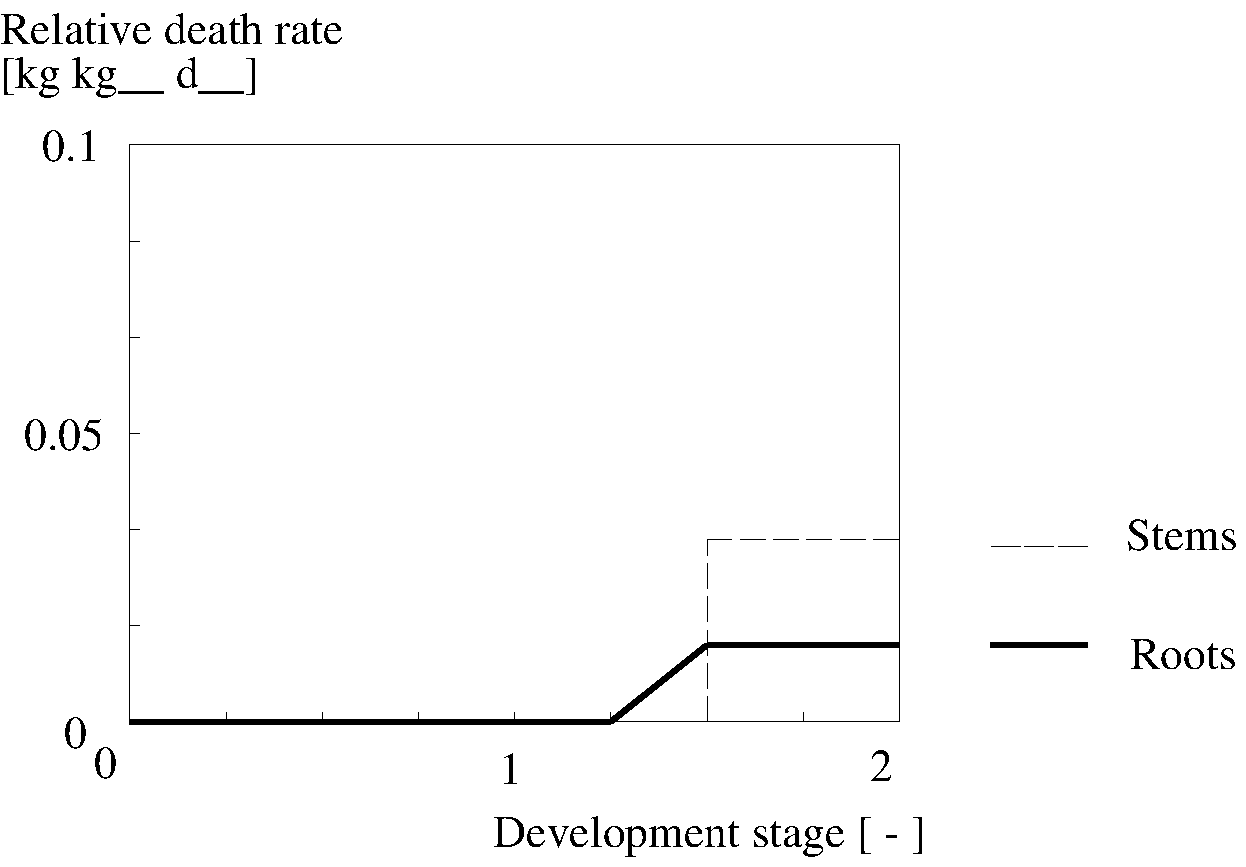
\includegraphics[width=100mm]{\FigDir/RDRRTB.pdf}
	\caption{Death rate of roots and stems as a function of development rate}
	\label{fig:DeathRoots}
	%\begin{forcewidth}{10.05cm}
	% \begin{center}\InputPS{\FigDir/RDRRTB.eps} \end{center}
	%\end{forcewidth}
\end{figure}


The net growth rate of the stems and roots can described by:

\begin{equation}
\label{eq:5.48}
\Delta Wn _{i~} =~\,\,\Delta W _{i~} -~ {\rm \dag } _{i} \,\, W _{i} 
\end{equation}

Where:\\[5pt]
\begin{tabularx}{\textwidth}{llXr}
	$\Delta$Wn$_{{\rm i}}$ &:& Net dry matter growth rate of organ i   &
	[kg ha$^{{\rm -1}}$ d$^{{\rm -1}}$]\\
	$\Delta$W$_{{\rm i}}$ &:& Dry matter growth rate of organ i (see eq. \ref{eq:5.45})   &
	[kg ha$^{{\rm -1}}$ d$^{{\rm -1}}$]\\
	W$_{{\rm i}}$ &:& Dry matter weight organ i  &
	[kg ha$^{{\rm -1}}$]\\
	\dag $_{{\rm i}}$ &:& Death rate organ i   &
	[kg kg$^{{\rm -1}}$ d$^{{\rm -1}}$]\\
	i &:& Stems (st), roots (rt)\\
\end{tabularx}

The death rates of stems and roots are crop specific and should be provided by the user.
A dependency of the development stage is assumed. AFGEN tables (acronym: {\bf RDRRTB}
(rt), {\bf RDRSTB} (st)) with the development stage as the independent variable are used to
describe this dependency.

Although the process which describes the death rate of leaves is more complicated than
the calculation of the death rate of stems and roots, the calculation to establish the total
dry weight of living leaves is the same as the computation of the dry matter weight of
stems and roots. The total dry matter weight of living leaves, stems and roots can be
found by integration over time of the net dry matter growth, $\Delta$Wn$_{{\rm i}}$, yields 
the dry matter.

\begin{equation}
\label{eq:5.49}
W _{t,i} ~=~W _{t-1\, ,\, i} ~+~\Delta Wn _{i} \,\Delta t
\end{equation}

Where:\\[5pt]
\begin{tabularx}{\textwidth}{llXr}
	W$_{{\rm i,t}}$ &:& Dry matter weight organ i at time step t   &
	[kg ha$^{{\rm -1}}$]\\
	$\Delta$Wn$_{{\rm i}}$ &:& Net dry matter growth rate of organ i   &
	[kg ha$^{{\rm -1}}$ d$^{{\rm -1}}$]\\
	$\Delta$t &:& Times step   &
	[d]\\
	i &:& Stems (st), roots (rt), leaves (lv)\\
\end{tabularx}

The equation \ref{eq:5.49} is recursive. In the model, the initial values of the dry weight of the
various organs are calculated. An initial value for the total dry weight of the crop
(acronym: {\bf TDWI}) should be provided by the user. This value is multiplied by the
partioning factors, pc$_{{\rm i}}$, at emergence, yielding the initial values of dry weight of the
various organs.

\subsection{Growth of leaves}
The area of green leaves is the major determinant for light absorption and photosynthesis
of the crop. Under optimal conditions, light intensity and temperature are the environmental factors influencing the rate of leaf area expansion. Light intensity determines the
rate of photosynthesis and hence the supply of assimilates to the leaves.

Temperature affects the rates of cell division and extension (Ng \& Loomis, 1984; Sheehy
{\it et al.}, 1980; Acock {\it et al.}, 1978). During the early stages of crop growth, temperature is
the overriding factor. The rate of leaf appearance and final leaf size are constrained by
temperature through its effect on cell division and extension, rather than by the supply of
assimilates (Hunt, 1982; Causton \& Venus, 1981; van Dobben, 1962). The growth curve
in the early stage has an exponential form. Some unpublished field data have shown that
the exponential model should be restricted to the situation where the development stage, 
D$_{{\rm s,t}}$ $<$ 0.3 and LAI $<$ 0.75 (see also eq. \ref{eq:5.4}). In the model, however, it is assumed that
the exponential growth rate of the leaf area index is valid until the source-limited increase
of the leaf area index equals the exponential growth rate.

The growth rate of the leaf area index per time step in the early, exponential growth
stage, can be calculated as:

\begin{equation}
% eq:5.50
L _{Exp,t} ~=~LAI _{{t~RL~T}_{e}}
\end{equation}

Where:\\[5pt]
\begin{tabularx}{\textwidth}{llXr}
	L$_{{\rm Exp,t}}$ &:& Growth rate of the leaf area index at time step t
	during exponential growth stage   &    [ha ha$^{{\rm -1}}$ d$^{{\rm -1}}$]\\
	LAI$_{{\rm t}}$ &:& Leaf area index at time step t    &
	[ha ha$^{{\rm -1}}$]\\
	RL &:& Maximum relative increase of leaf area index   &
	[\degrees C$^{{\rm -1}}$ d$^{{\rm -1}}$]\\
	T$_{{\rm e}}$ &:& Daily effective temperature (see 5.2c)   &
	[\degrees C]\\
\end{tabularx}

In theory, the maximum relative increase of the leaf area index, {\bf RL}, is a function of
effective temperature. For a relative wide range of temperatures {\bf RL} responds more or
less linearly to temperature (Hunt {\it et al.}, 1985; Causton \& Venus, 1981; van Dobben,
1962). In the model however, a fixed value per crop type is assumed (acronym: 
{\bf RGRLAI}). This value should be given by the user.

The accumulated leaf area index at time step t during the exponential growth stage can be
described as:

\begin{equation}
\label{eq:5.51}
LAI _{t~} =~LAI _{t-1} ~+~L _{Exp\, ,\, t} ~\Delta t
\end{equation}

Where:\\[5pt]
\begin{tabularx}{\textwidth}{llXr}
	L$_{{\rm Exp,t}}$ &:& Growth rate of the leaf area index at time step t
	during exponential growth stage    &    [ha ha$^{{\rm -1}}$ d$^{{\rm -1}}$]\\
	LAI$_{{\rm t}}$ &:& Leaf area index at time step t   &
	[ha ha$^{{\rm -1}}$]\\
	$\Delta$t &:& Time step   &    [d]
\end{tabularx}

The equation\ref{eq:5.51} is recursive. In the model, {\bf LAI$_{{\rm t}}$} is initialized by 
setting the starting
value equal to the leaf area index at emergence (acronym: {\bf LAIEM}). The leaf area index
at emergence is crop specific and should be provided by the user.

During the development of the crop, leaf area expansion is increasingly restricted by
assimilate supply (i.e. source limited increase). Branching and tillering generate an
increasing number of sites per plant, where leaf initiation can take place. As mentioned
earlier, in the model it is assumed that the exponential growth rate of leaf area index will
continue until it equals the source limited growth rate of the leaf area index.

The growth rate of the leaf area index at time step t during the source limited growth 
stage can be described by:

\begin{equation}
\label{eq:5.52}
L _{Sc,t} ~=~\Delta Wn _{lv} ~S _{la} 
\end{equation}

Where:\\[5pt]
\begin{tabularx}{\textwidth}{llXr}
	L$_{{\rm Sc,t}}$ &:& Growth rate of the leaf area index at time step t
	during the source limited growth stage    &
	[ha ha$^{{\rm -1}}$ d$^{{\rm -1}}$]\\
	$\Delta$Wn$_{{\rm lv}}$ &:& Net dry matter growth of leaves at time step t    &
	[kg ha$^{{\rm -1}}$ d$^{{\rm -1}}$]\\
	S$_{{\rm la}}$ &:& Specific leaf area at time step t   &
	[ha kg$^{{\rm -1}}$]\\
\end{tabularx}

The net dry matter growth of leaves, $\Delta$Wn$_{{\rm lv}}$, can be found by subtracting the weight of
leaves which died during the current time step from the dry matter growth of leaves,
$\Delta$W$_{{\rm lv}}$. This process will be described later in more detail in this paragraph.

The specific leaf area, {\bf S$_{{\rm la}}$} (acronym: {\bf SLATB}), is defined as the increase of the leaf area
of the crop per kg weight increase of the living leaves. S$_{{\rm la}}$ is crop specific and a function
of the development stage (see figure 8). In the model this dependency is described using
an AFGEN table with the development stage as the independent variable (see also
Appendix 2).

The accumulated leaf area index at time step t during the source limited growth stage can
be described as:

\begin{equation}
\label{eq:5.53}
LAI _{t~} =~LAI _{t-1} ~+~L _{Sc\, ,\, t} ~\Delta t
\end{equation}

Where:\\[5pt]
\begin{tabularx}{\textwidth}{llXr}
	L$_{{\rm Sc,t}}$ &:& Growth rate of the leaf area index at time step t
	during the source limited growth stage     &   [ha ha$^{{\rm -1}}$ d$^{{\rm -1}}$]\\
	LAI$_{{\rm t}}$ &:& Leaf area index at time step t     &
	[ha ha$^{{\rm -1}}$]\\
	$\Delta$t &:& Time step    &    [d]\\
\end{tabularx}

The equation \ref{eq:5.53} is recursive. In the model, {\bf LAI$_{{\rm t}}$} is initialized by 
setting the starting
value equal to the leaf area index at emergence (acronym: {\bf LAIEM}). The leaf area index
at emergence is crop specific and should be provided by the user.

In the model, however, the accumulated leaf area cannot be calculated directly. The leaf
area index has to be corrected for leaf senescence which occurred during the current time
step. The leaf senescence can be caused by physiological ageing, water stress and/or high
leaf area index (i.e. mutual shading). Later in this text, more attention will be paid to
these effects.

In order to correct for leaf senescence, the specific leaf area of each time step, S$_{{\rm la}}$, the
growth of the dry matter weight of leaves per time step, $\Delta$W$_{{\rm lv}}$ and the physiological age,
P$_{{\rm age}}$ (see eq. \ref{eq:5.57}), have to be stored in three different arrays. These arrays are organized
as follows: the first element of the arrays represents the most recent age class (or time
step) and the last element of the arrays represents the oldest age class (or time step). It
should be clear that the position of an element in the arrays represents its age class, in
time steps. The dry matter weight of the leaves, which have died during the current time
step, has to be. subtracted from the growth of dry matter weight per time step. One array
contains thus the net dry matter growth of the leaves per time step, $\Delta$Wn$_{{\rm lv}}$. 
The procedure which describes this process will be explained later in this text. 

After the correction for leaf senescence, the accumulated leaf area can be established. The
net dry matter weight of the leaves, $\Delta$Wn$_{{\rm lv,}}$  in the remaining and new leaf classes is
multiplied with the specific leaf areas (see eq. \ref{eq:5.52}) to get the growth rate of the leaf area
index of the living leaves per age class. Multiplication with $\Delta$t and summation over the
classes (eq. \ref{eq:5.53}) yields the total leaf area index. The green area index of the stems and
the storage organs is added to this amount. The total dry matter weight of living leaves
can be found in a similar way by using equation \ref{eq:5.49}.

\begin{figure}[p]
	%Fig. 5.8   
	\centering
	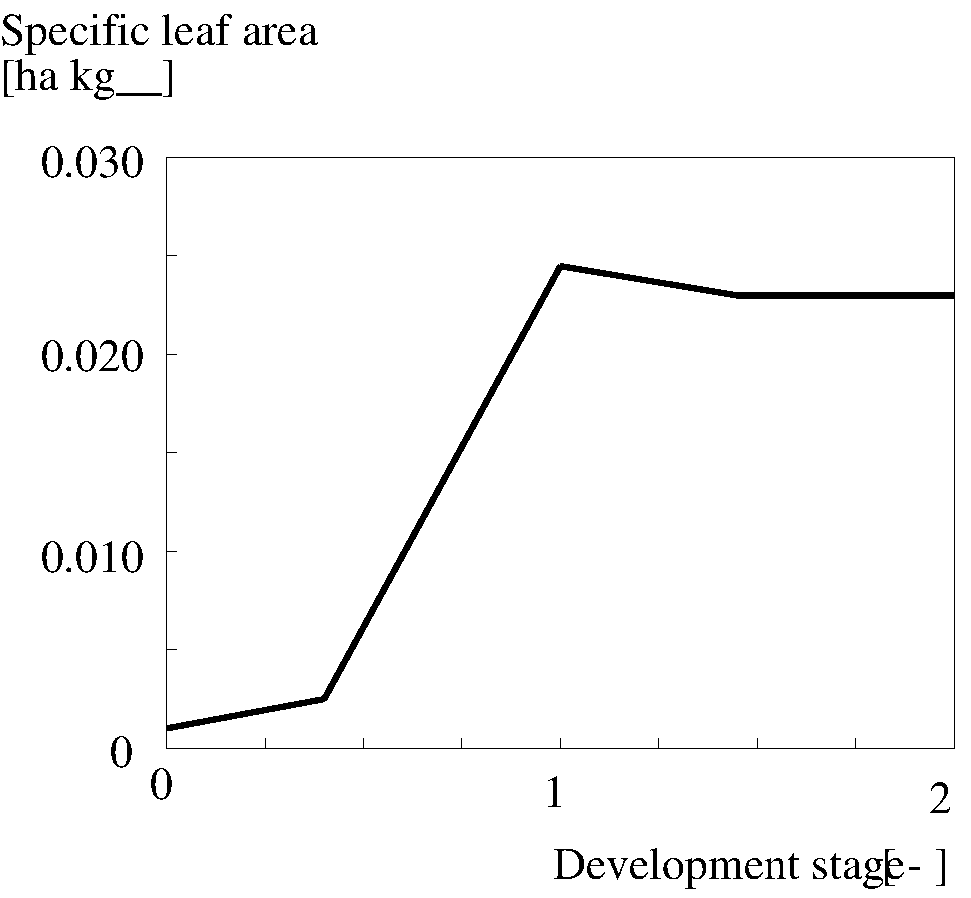
\includegraphics[width=120mm]{\FigDir/SLATB.pdf}
	\caption{Specific leaf area as a function of development stage}
	\label{fig:SpecificLeafArea}
	%\begin{forcewidth}{10.05cm}
	% \begin{center}\InputPS{\FigDir/SLATB.eps} \end{center}
	%\end{forcewidth}
\end{figure}

As is mentioned earlier, the green area index of the stems and storage organs, may absorb
a substantial amount of radiation. Therefore it should be added to the total leaf area
index. The green area index of these organs can be calculated by:

\begin{equation}
% eq:5.54
GAI_{i} ~=~SS _{i} W _{i} 
\end{equation}

Where:\\[5pt]
\begin{tabularx}{\textwidth}{llXr}
	GAI$_{{\rm i}}$ &:& Green area index of organ i    &
	[ha ha$^{{\rm -1}}$]\\
	SS$_{{\rm i}}$ &:& Specific green area of organ i    &
	[ha kg$^{{\rm -1}}$]\\
	W$_{{\rm i}}$ &:& Dry matter organ i (see eq. \ref{eq:5.49})    &
	[kg ha$_{{\rm -1}}$]\\
	i &:& Stems (st), storage organs (so)\\
\end{tabularx}

The specific green area of stems (acronym: {\bf SSA}) and storage organs (acronym: {\bf SPA}) are
crop specific and should be provided by the user. The specific storage organ area is also
known as the specific pod area.

Special attention should be paid to the fact that during the exponential growth stage, the
specific leaf is not established. Therefore, during this period, for each time step, the
specific leaf area has to be calculated according to:

\begin{equation}
% eq:5.55
S_{\exp,t} ~=~ {\frac{L_{\exp,t}}{\Delta W_{lv} }}
\end{equation}

Where:\\[5pt]
\begin{tabularx}{\textwidth}{llXr}
	S$_{{\rm exp,t}}$ &:& Specific leaf area at time step t during the 
	exponential growth stage    &     [ha kg$^{{\rm -1}}$]\\
	$\Delta$W$_{{\rm lv}}$ &:& Dry matter increase of leaves (see eq. \ref{eq:5.45})   &
	[kg ha$_{{\rm -1}}$ d$^{{\rm -1}}$]\\
	L$_{{\rm \exp,t}}$ &:& Growth rate of the leaf area index at time step t
	during exponential growth stage (see eq. \ref{eq:5.51})   &
	[ha ha$^{{\rm -1}}$ d$^{{\rm -1}}$]\\
\end{tabularx}


In de model, it is assumed that senescence does not occur during the exponential growing
stage. This means that $\Delta$W$_{{\rm lv}}$ can be used in stead of the net dry matter growth, $\Delta$Wn$_{{\rm lv}}$.

\subsection{Death of leaves (senescence)}
As stated before, leaf senescence is more complicated. Senescence refers to the loss of
capacity to carry out essential physiological processes and to the loss of living biomass.
The fundamental processes involve physiological ageing and protein breakdown. These
processes are difficult to quantify. Leaves are assumed to die when they have completed
their life cycle. The dying rate may be accelerated as a result of drought stress or of
mutual shading.

{\it physiologic ageing}\\
Leaves die due to exceedance of the life span for leaves (i.e. physiologic ageing). Life
span is defined as the maximum time in days a leaf can live at a constant temperature of
35\degrees C. Life span is crop specific. The concept of lifespan is compatible with a definition
in terms of temperature sum as given by Gallagher (1979).
The physiologic ageing factor per time step can be calculated as:

\begin{equation}
% eq:5.56
f _{rai} ~=~{\frac{ T~-~T _{b\, ,\, age} }{35~-~ T _{b\, ,\, age} }}
\end{equation}

Where:\\[5pt]
\begin{tabularx}{\textwidth}{llXr}
	f$_{{\rm rai}}$ &:& Physiologic ageing factor for leaf age increase   &
	[-]\\
	T &:& Daily (average) temperature   &
	[\degrees C]\\
	T$_{{\rm b,age}}$ &:& Lower threshold temperature for physiologic ageing   &
	[\degrees C]\\
\end{tabularx}

The lower threshold temperature for physiologic ageing, {\bf T$_{{\rm b,age}}$} (acronym: {\bf TBASE}), is
crop specific and should be provided by the user. The integral of the physiologic ageing
factor over time yields the physiologic age. 

\begin{equation}
\label{eq:5.57}
P _{age,t} ~=~ P _{age,t-1} ~+~f_{rai} \Delta t
\end{equation}

Where:\\[5pt]
\begin{tabularx}{\textwidth}{llXr}
	P$_{{\rm age,t}}$ &:& Physiologic age at time step t & [d]\\
	f$_{{\rm rai}}$ &:& Physiologic ageing factor for leaf age increase & [-]\\
	$\Delta$t &:& time step & [d]\\
\end{tabularx}

Leaves may attain the age defined by the crop specific life span (acronym: {\bf SPAN}).
However, as is mentioned earlier, they can not exceed it. In the model the ages of the
leaf classes are checked. The first class younger than the defined life span becomes the
oldest class. Note that death of old leaves takes place after ageing, being the result of the
daily shifting from one leaf class to the next (Johnson \& Thornley, 1983). In this way,
the life time of leaves is the maximum number of days that a leaf class contributes to the
LAI and to photosynthesis.

{\it Death rate due to water stress}\\
The potential death rate of leaves due to water stress can be calculated as:

\begin{equation}
% eq:5.58
\Delta W_{d}^{1} ~=~ W_{lv} \, (\, 1\, -\,{\frac{T _{a} }{T _{p} }} \, )\, {\rm \dag } _{\max ,lv} 
\end{equation}

Where:\\[5pt]
\begin{tabularx}{\textwidth}{llXr}
	$\Delta$W$^{{\rm 1}}$$_{{\rm d}}$ &:& Potential death rate of leaves due to water stress   &
	[kg  ha$^{{\rm -1}}$ d$^{{\rm -1}}$]\\
	\dag $_{{\rm max,lv}}$ &:& Maximum relative death rate of leaves due to
	water stress   &     [kg kg$^{{\rm -1}}$ d$^{{\rm -1}}$]\\
	W$_{{\rm lv}}$ &:& Dry matter weight of the leaves (see eq. \ref{eq:5.49})  &
	[kg ha$^{{\rm -1}}$]\\
	T$_{{\rm a}}$ &:& Actual transpiration (see \S \ref{sec:evapotranspiration})    &
	[cm d$^{{\rm -1}}$]\\
	T$_{{\rm p}}$ &:& Potential transpiration (see \S \ref{sec:evapotranspiration})   &
	[cm d$^{{\rm -1}}$]\\
\end{tabularx}

The maximum relative death rate of leaves due to water stress, {\bf \dag $_{{\rm max,lv}}$} 
(acronym: {\bf PERDL}) is crop specific and should be provided by the user.

{\it Death rate due to high leaf area index}\\
Leaf senescence also occurs due to high leaf area index (i.e. mutual shading). A relative
death rate due to self$-$shading is defined which increases linearly from zero at a certain,
critical leaf area index, to its maximum value at twice this critical leaf area index. Typical
values for the maximum relative death rate and the critical LAI are 0.03 d$^{{\rm -1}}$ and 4 
ha ha$^{{\rm -}{1}}$, respectively (Spitters {\it et al.} 1989).

The potential death rate of leaves due to high LAI can be calculated as:

\begin{equation}
% eq:5.59
\Delta W_{d}^{2} ~=~ W_{lv} \cdot 0.03 \cdot {\frac{LAI - LAI_c}{LAI_c}}
\end{equation}

Where:\\[5pt]
\begin{tabularx}{\textwidth}{llXr}
	$\Delta$W$^{{\rm 2}}$$_{{\rm d}}$ &:& Potential death rate of leaves due to 
	high LAI   &    [kg ha$^{{\rm -1}}$ d$^{{\rm -1}}$]\\
	W$_{{\rm lv}}$ &:& Dry matter weight of the leaves  &  [kg ha$^{{\rm -1}}$]\\
	LAI &:& Leaf area index   &    [ha ha$^{{\rm -1}}$]\\
	LAI$_{{\rm c}}$ &:& Critical leaf area index   &     [ha ha$^{{\rm -1}}$]\\
\end{tabularx}

The critical leaf area index, LAI$_{{\rm c}}$, can be computed by:

\begin{equation}
% eq:5.60
LAI_{c} = {\frac{3.2}{\kappa_{df} }}
\end{equation}

Where:\\[5pt]
\begin{tabularx}{\textwidth}{llXr}
	LAI$_{{\rm c}}$ &:& Critical leaf area index    &    [ha ha$^{{\rm -1}}$]\\
	$\kappa$$_{{\rm df}}$ &:& Extinction coefficient for 
	the diffuse radiation flux   &    [-]\\
\end{tabularx}

The last term of the right hand side of the equation 5.59 must be between 0 and 0.03. A 
value lower than 0 will be set to 0 and a value higher than 0.03 will be set to 0.03. In the
model, the highest value of the two calculated potential death rates of leaves, 
$\Delta$W$^{{\rm 1}}$$_{{\rm d}}$ and $\Delta$W$^{{\rm 2}}$$_{{\rm d}}$, is selected 
for further calculations of the reduction of dry matter weight increase,
per time step of the leaf classes, as is will be explained now. 

The weight of leaves which have died during the current time step, can be calculated by
multiplying the death rate (due to water stress and/or high LAI), with the time step.

\begin{equation}
% eq:5.61
W_{d} = \max(\Delta W_{d}^{1} , \Delta W_{d}^{2})\cdot \Delta t
\end{equation}

Where:\\[5pt]
\begin{tabularx}{\textwidth}{llXr}
	W$_{{\rm d}}$ &:& Weight of leaves that have died during 
	current time step    &    [kg ha$^{{\rm -1}}$]\\
	$\Delta$W$^{{\rm 1}}$$_{{\rm d}}$ &:& Potential death rate of leaves due 
	to water stress   &      [kg ha$^{{\rm -1}}$ d$^{{\rm -1}}$]\\
	$\Delta$W$^{{\rm 2}}$$_{{\rm d}}$ &:& Potential death rate of leaves due to 
	high LAI   &     [kg ha$^{{\rm -1}}$ d$^{{\rm -1}}$]\\
	$\Delta$t &:& Time step    &    [d]\\
\end{tabularx}

The weight of the leaves which have died, W$_{{\rm d}}$, is subtracted from the weight of the oldest
leaf class. If there is only one class the result should be positive. When more leaf classes
exist, the oldest leaf class may be emptied completely, the remainder is subtracted from
the next leaf class. Emptying the oldest leaf class goes on, until the original amount is
dissipated completely and the remaining amount of leaves remains positive. All leaves are
shifted every time step (daily) to the next class.

\subsection{Root growth}
\label{sec:rootgrowth}

Growth of roots in terms of depth is implemented in a straightforward way in WOFOST. 
The model assumes that at the start of the crop simulation, the crop has an initial rooting 
depth which is usually set to 10 cm. After initialization, the crop grows with a fixed daily 
increase in rooting depth until either a crop-specific maximum depth or a soil-defined maximum 
depth is reached. In versions of WOFOST that implement a shallow groundwater table, the 
increase in root depth will also cease if the roots are within 10cm of the groundwater 
table and the crop cannot form airducts. WOFOST does not define a root density profile 
and assumes that plant roots can subtract water equally from the entire rooted layer.

Growth of roots in terms of biomass follows the same logic as other plant organs in that
the roots receive a fraction of the net daily assimilates based on the partitioning 
fraction to roots for that day. Similar to stems, death of root material depends on 
the development stage through a relative death rate that causes a fraction of the 
roots to die after a certain development stage.

In the model there is no relationship between the amount of biomass partitioned to the roots 
and the increase of the depth of the roots, with the exception that the increase in root
depth will cease if there is no partitioning of biomass to roots anymore. Also there is 
no impact of environmental conditions (such as drought) on root growth.

In the model, root growth is implemented in a straightforward way. One needs to specify
the following crop and soil specific parameters:
\begin{itemize}
	\item Initial rooting depth, {\bf RD$_{{\rm i}}$} (acronym: {\bf RDI});
	\item Maximum rooting depth determined by the crop, {\bf RD$_{{\rm crop}}$} (acronym: {\bf RDMCR});
	\item Maximum daily increase in rooting depth, {\bf RR$_{{\rm max}}$} (acronym: {\bf RRI});
	\item Maximum rooting depth determined by the soil, {\bf RD$_{{\rm soil}}$} (acronym: {\bf RDMSOL}).
\end{itemize}

The daily increase of the rooting depth is a function of development stage and is crop
specific. The root growth can be calculated as:

\begin{equation}
% eq:5.62
\Delta RD~=~RR_{\max} \cdot \Delta t
\end{equation}

Where:\\[5pt]
\begin{tabularx}{\textwidth}{llXr}
	$\Delta$RD &:& Increase of the rooting depth   &   [cm]\\
	RR$_{{\rm max}}$ &:& Maximum daily increase in rooting depth  &  [cm d$^{{\rm -}{1}}$]\\
	$\Delta$t &:& Time step   &  [d]\\
\end{tabularx}

In the model it is assumed that the extension growth of the roots continues until the
maximum rooting depth is reached. The rooting depth can be established by:

\begin{equation}
% eq:5.63
RD _{t~} =~RD _{t-1} ~+~\Delta RD
\end{equation}

Where:\\[5pt]
\begin{tabularx}{\textwidth}{llXr}
	RD$_{{\rm t}}$ &:& Rooting depth at time step t   &  [cm]\\
	$\Delta$RD &:& Increase of the rooting depth    & [cm]\\
\end{tabularx}

In the model, the maximum rooting depth is established by taking the lowest value of the\\
maximum rooting depth determined by the crop, RD$_{{\rm crop}}$, the maximum rooting depth
determined by the soil, RD$_{{\rm soil}}$, and the depth the roots would reach in the potential
production situation. It is assumed that the maximum rooting depth is always equal or
higher than the initial rooting depth.

In theory, extension growth of the roots ceases when no more assimilates are available,
when an impermeable layer in the profile is reached, when the root tip reaches a soil
compartment with a moisture content at or below wilting point (Salim {\it et al.}, 1965) or
when the root tip reaches the groundwater table. This last situation only occurs in case
the crop cannot form airducts. In the model, however, only the following situations are
distinguished. The root extension stops when no more assimilates are available, but then
the complete simulation process ceases (eq. \ref{eq:5.47}). Root extension also stops, when the
root tip comes within ten centimeters of the groundwater table and the crop cannot form
airducts. The user should provide information if the crop can produce airducts (acronym:
{\bf IAIRDU}) or not.



%\chapter{SIMULATION OF CONTINUOUS PROCESSES}

This chapter introduces the principles of Euler integration and the method adopted to
couple different subprocesses without transgressing the rules of Euler integration. It is
based on the work of van Kraalingen (1991). A basic knowledge of the state variable
approach, as it is used in continuous simulation, is assumed (see e.g. van Kraalingen,
1991; Penning de Vries \& van Laar, 1982; de Wit \& Goudriaan, 1978).

Various integration methods can be used in the simulation of continuous systems, ranging
from simple rectangular integration (Euler) to higher order integration algorithms 
(trapezoidal, Runge-Kutta, etc.), possibly with a variable time step. From the point of 
view of program structure, a program that accommodates Euler integration only, is less 
complicated and easier to understand than one accommodating higher order methods of 
integration. However, this less complicated structure requires changes to be made in the
integration section of the simulating subroutines to allow higher order integration methods
to be used (see Rappoldt \& van Kraalingen 1990). The simulation of crop growth in
FORTRAN often uses Euler integration with a fixed time step (i.e. 1 day) because it
makes the program structure is less complicated and more understandable. Figure \ref{fig:euler}
shows the correct order in which calculations should be executed when Euler integration
is used:

\begin{figure}[p]
% Fig 3.1
\centering
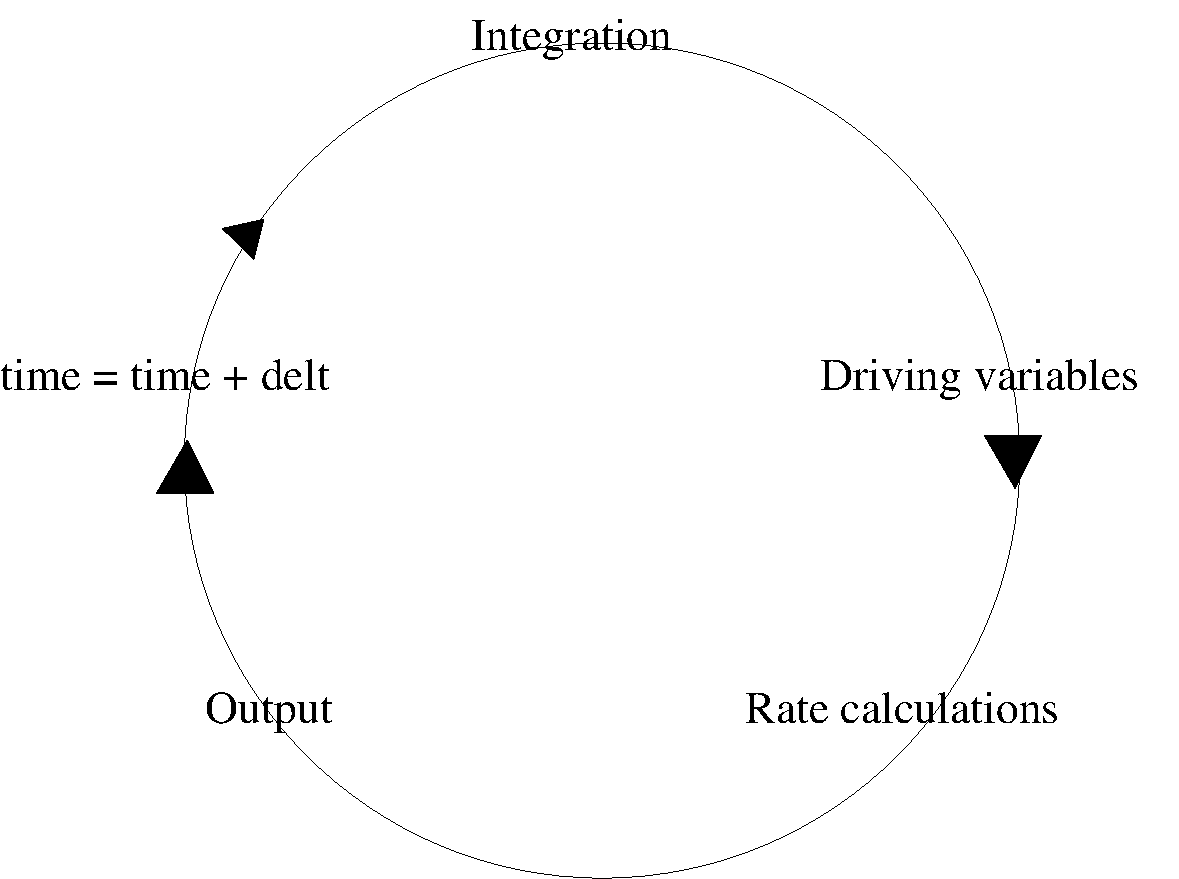
\includegraphics[width=140mm]{\FigDir/FSE0.pdf}
\caption{Order of calculations when simulating continuous systems using Euler 
         integration (van Kraalingen, 1991)}
\label{fig:euler}
\end{figure}

Note that in this sequence, at the point where output is generated, state variables and rates
of change correspond to the time for which they were calculated. 

In theory, the sequence in which various state variables are updated, is not important
because their values should not depend on each other but should be fully determined by
the rate variables. In practice, however, state variables may sometimes be derived from
other state variables (e.g. root/shoot ratio or total weight of leaves equals weight of dead
leaves plus weight of green leaves). It is important to put the state calculations and rate
calculations in the right order.

To ensure that the results of the simulation are correct, the different types of calculations
(integration, driving variables and rate calculations) should be strictly separated. All states
should be updated, then all driving variables should be calculated, after which all rates of
change can be determined. If this rule is not applied rigorously, there is a risk that some
rates will pertain to states at the current time whereas others will pertain to states from
the previous time step.

Since the calculations of rates and states cannot be mixed during a time step but should be
executed separately, all the state calculations have to be merged into one block as do all
the rate calculations. Often, different subprocesses are interacting. In many cases these
interactions among the subprocesses are only weak. The water content at different depths
in the soil, for example, is needed for the plant/soil system in the plant submodel. This is
then used to determine water uptake for transpiration in dependence of rooting depth. The
submodels for the plant and soil water thus share a limited amount of information,
however, they may contain very detailed descriptions of plant growth and soil moisture
redistribution with many different rate and state calculations.

In view of the above, it is not a good solution to combine all the state calculations from
the different subprocesses into one large program section and all the rate calculations in
another. But it is feasible to separate the state and rate calculations within the subprocess
descriptions and have a calling program decide which of the two to execute. With this
method, the states can be calculated separately from the rates, whereas rates and states
pertaining to the same subprocess are within the same subprogram. This technique is also
discussed by van Kraalingen and Rappoldt (1989).

This concept of 'task-controlled execution' is illustrated in figure \ref{fig:fse_struct} The program lines
of the plant and soil water subprocesses are separated into rate and state sections and only
one of these is executed during a single call. Note that this program structure performs
the calculations in exactly the same order as the circle given in figure \ref{fig:euler}.

So far, the initialization of the states variables or where to enter the simulation circle and
where to leave it, is not discussed, (see figure \ref{fig:euler}). It is convenient to leave the circle
somewhere between time update and integration, because there the time and corresponding 
rates have been written to the output device and after the time update it seems logical
to check whether the finish time (end date of simulation) has been exceeded or whether
further simulation is required. Consequently, the circle should also be entered between
time update and integration.

The most convenient way to initialize the subprocesses is to have this operation controlled
by the main program. This makes reruns possible, because in the main  program the
whole model can be reset to its initial state and be run again, with different weather data
for instance. These refinements to figure \ref{fig:euler} are shown in figure \ref{fig:fse_order}.

\begin{figure}[p]
%fig 3.2
\centering
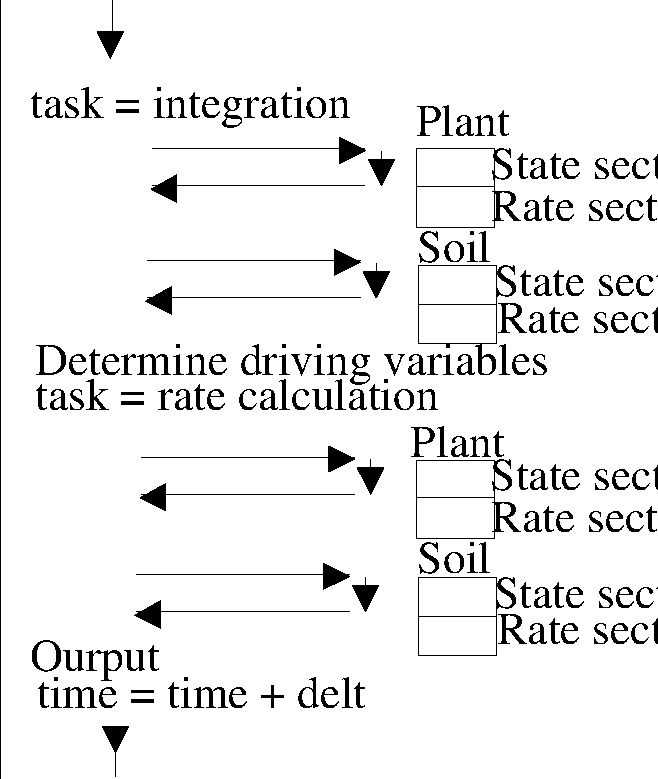
\includegraphics[width=140mm]{\FigDir/FSE1.pdf}
\caption{General structure for incorporating several subprocesses 
containing integration and rate calculation into a single simulation model (van Kraalingen,
1991).}
\label{fig:fse_struct}
\end{figure}

The question mark between time = time+delt and integration in figure \ref{fig:fse_order}, indicates the
point at which it is decided whether or not to execute another time step. If the decision is
"no", the model proceeds to the terminal section; if it is "yes" the circle is run once
more. After proceeding to the terminal section, it must be decided whether a rerun is
required. If the decision is "yes" the model has to be re-initialized and a new simulation
run is started.

As shown in figure \ref{fig:fse_order}, the modularity of the subprocess descriptions is preserved by
introducing the concept of task-controlled execution (the calling program decides what the
subroutine should do: either integration or rate calculation). To be able to do reruns, the
various subprocess descriptions that can also be driven by the task variable have to be
initialized externally, and some terminal calculations (e.g. harvest index) have to be done.
Therefore, a subprocess in the program should recognize four different tasks: {\bf Initialization}, 
{\bf Integration}, {\bf Rate Calculation} and {\bf Terminal Calculation}.

\begin{figure}[p]
%Fig. 3.3 
\centering
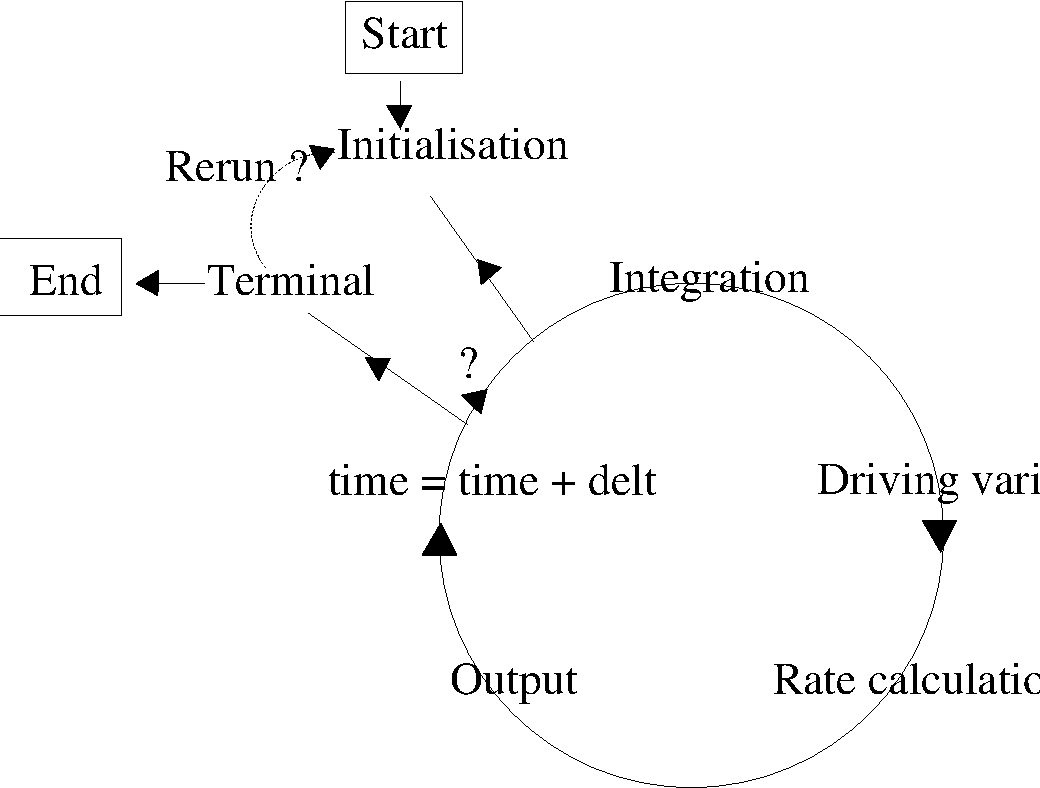
\includegraphics[width=140mm]{\FigDir/FSE2.pdf}
\caption{Order of calculations when simulating continuous systems using Euler
integration, illustrating where to enter and leave the circle and how reruns
are implemented (van Kraalingen, 1991)}
\label{fig:fse_order}
\end{figure}

A consequence of this structure, the first step after initialization is integration. This does
no harm if the rates have been set to zero explicitly, so that the first integration has no
effect on the value of the states. In practice this means incorporating many rate assignments 
which are set equal to zero into the model. To avoid this, integration can be
skipped if the previous task was initialization (during which the states have been assigned
values anyway). The subsequent rate calculation will then use the state variables to
initialize the rates of change.

It should be noted that there exists a clear distinction between the use of the Euler
integration and the Gaussian integration, which is used extensively in chapters five and
six. See also Appendix 1. The Euler integration is used to integrate the processes on a
larger scale than the Gaussian method. The Euler integration as discussed above, is used
to integrate all the crop growth processes over the growing period (i.e. all the time steps
executed), while the Gaussian integration is used to integrate the individual processes over
for example depth, or one day (i.e one time step). 

The integration of the rate variables over time in order to get the state variables, is 
implemented as follows.

\begin{equation}
\label{eq:euler_integration}
Q _{t~} =~Q _{t-1} ~+~\Delta Q _{t} \,\Delta t
\end{equation}

Where:\\[5pt]
\begin{tabularx}{\textwidth}{llXr}
 Qt &:& State variable at time step t    &   [unit]\\
 $\Delta$Q$_{{\rm t}}$ &:& Rate variable at time step t   &    [unit d$^{{\rm -1}}$]\\
 $\Delta$t &:& Time step   &    [d]\\
\end{tabularx}

%\include{chapter4}
%\chapter{CROP}

\section{Overview of the crop growth model}

The WOFOST model describes phenological development, growth and yield formation of
a crop from emergence till maturity on the basis of crop genetic properties and 
environmental conditions. The model simulates dry matter accumulation of a crop as a function
of irradiation, temperature and crop characteristics in time steps of one day. 
The basis for calculating dry matter production, is the rate of gross CO$_{{\rm 2}}$ assimilation of
the canopy. This rate is dependent on the radiation energy absorbed by the canopy, which
is a function of incoming radiation and of crop leaf area. From the absorbed radiation and
the photosynthetic characteristics of single leaves, the daily rate of CO$_{{\rm 2}}$ assimilation of the
crop is calculated. Part of the carbohydrates produced (CH$_{{\rm 2}}$O) are used to provide energy
for the maintenance of the existing live biomass (maintenance respiration). The remaining
carbohydrates are converted into structural matter. In this conversion, some of the weight
is lost as growth respiration. The growth rate is thus obtained as:

\begin{equation}
% eq 5.1
\Delta W ~=~ C _{e} ~( A ~-~ R _{m} )
\end{equation}

Where:\\[5pt]
\begin{tabularx}{\textwidth}{llXr}
$\Delta$W &:& Growth rate    &   
    [kg Dry Matter ha$^{{\rm -1}}$ d$^{{\rm -1}}$]\\
A  &:& Gross assimilation   rate &  
    [kg CH$_{{\rm 2}}$O ha$^{{\rm -1}}$ d$^{{\rm -1}}$]\\
R$_{{\rm m}}$  &:& Maintenance respiration rate    &  
    [kg CH$_{{\rm 2}}$O ha$^{{\rm -1}}$ d$^{{\rm -1}}$]\\
C$_{{\rm e}}$ &:& Conversion efficiency off assimilates total crop   &   
    [kg Dry Matter kg$^{{\rm -1}}$ CH$_{{\rm 2}}$O]\\
\end{tabularx}

The dry matter produced is partitioned amongst the various plant organs such as roots,
leaves, stems and storage organs, using partitioning factors that are a function of the
phenological development stage of the crop (Spitters et al., 1989). The fraction partitioned
to the leaves, determines leaf area development and hence the dynamics of light interception. 
The dry weights of the plant organs are obtained by integrating their growth rates
over time (see eq. \ref{eq:euler_integration}).

Leaf mass is subdivided into age classes. During the development of the crop a part of
living biomass dies due to senescence. Some simulated crop growth processes are
influenced by temperature, like for example the maximum rate of photosynthesis and the
maintenance respiration. Other processes like the partitioning of assimilates or decay of
crop tissue are steered by the phenological stage. The phenological development stage is
calculated as a function of ambient temperature and possibly modified by the effect of day
length. An overview of all these processes was depicted in figure \ref{fig:CropGrowthProcesses} 
(\S \ref{sec:2.1}), which is repeated here below for easy reference. See figure \ref{fig:CropGrowthProc2}.

The simulation of phenological development and biomass formation is performed in
subroutine {\bf CROPSI} (general version) or {\bf CRSIM} (JRC version). The simulated processes
include the rate of phenological development, CO$_{{\rm 2}}$ assimilation, maintenance respiration,
dry matter partitioning resulting in biomass accumulation, growth and senescence of
leaves, transpiration and extension of roots. 

Elaborate calculations of rates of change are performed in specific subroutines called by
{\bf CROPSI} or {\bf CRSIM}. These routines are {\bf TOTASS} and {\bf ASSIM} for the daily assimilation
rate and {\bf EVTRA} for the evapotranspiration rates. All the equations used to describe these
processes are treated in the following sections.

\begin{figure}[p]
\centering
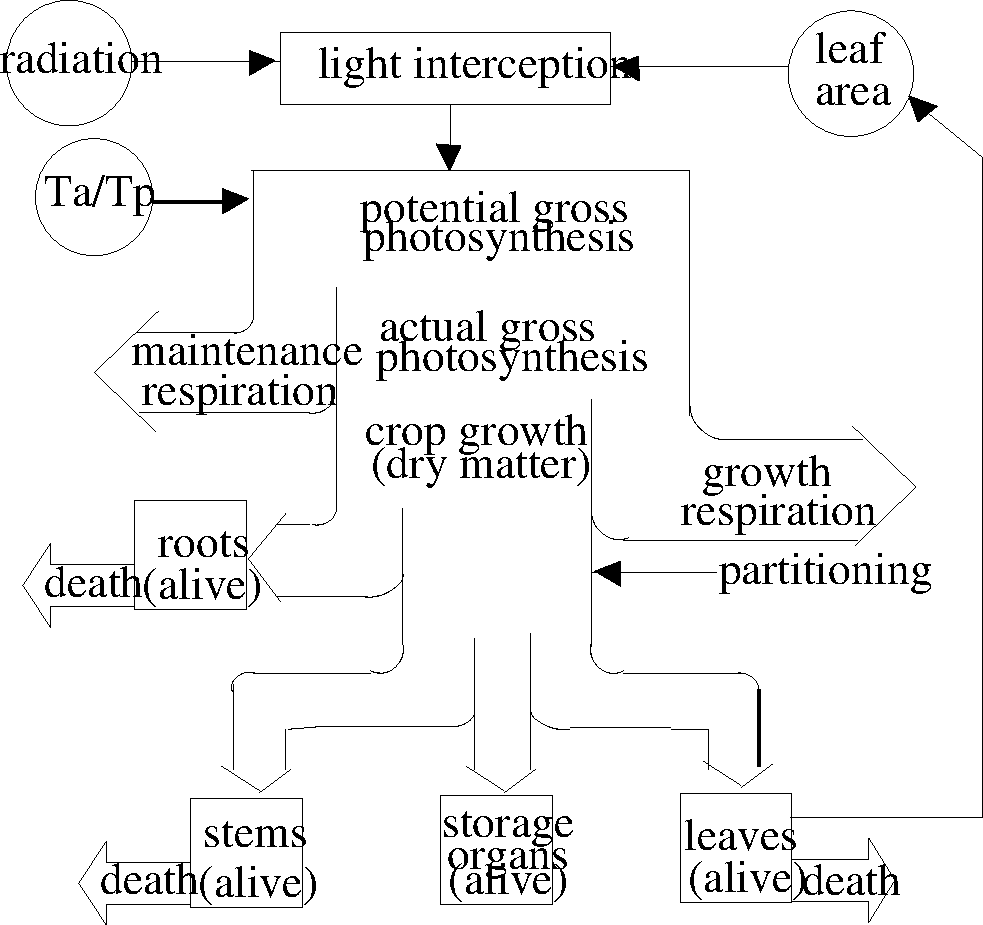
\includegraphics{\FigDir/ASIMTREE.pdf}
\caption{Crop growth processes. \small T$_{{\rm a}}$ and T$_{{\rm p}}$ are the actual and potential 
transpiration rate. (de Koning et al, 1993)}
\label{fig:CropGrowthProc2}
% \begin{center}\InputPS{\FigDir/ASIMTREE.eps} \end{center}
\end{figure}

\section{Phenological development of a crop}

The physiological age of a plant is defined by the development stage, which on its turn is
characterized by the formation of the various organs and their appearance. The most
important phenological change is the one from vegetative to the reproductive stage, which
determines the most important change in the dry matter allocation over organs. As many
physiological and morphological processes change with the phenological stage of the
plant, accurate quantification of phenological development is essential in any simulation
model for crop growth. For many annual crops, the development stage can conveniently
be expressed in a dimensionless variable, having the value 0 at seedling emergence, 1 at
flowering and 2 at maturity (van Heemst {\it et al.}, 1986a; 1986b). 

\subsection{Crop emergence}

As start of the growing season the date of sowing or of emergence can be chosen. For a
photosynthesis-driven model like WOFOST, the simulation of crop growth starts at
emergence. If the sowing date is chosen by the model user, the day of emergence is
determined by the model in subroutine {\bf CROPSI} or {\bf CRSIM}. The crop emergence can be
defined as a function of the effective daily temperature sum since sowing date. Emergence
takes place when the effective daily temperature sum reaches the threshold temperature
for emergence (acronym: {\bf TSUMEM}). This threshold temperature is crop specific and
should be given by the user. The daily effective temperature depends on the base
temperature, below which no phenological processes take place, and the maximum daily
temperature, beyond which the phenological activity does not increase anymore, are also
crop specific. An example of this effective daily temperature as a function of daily
average temperature is depicted in figure \ref{fig:TEFFMAX}.

\begin{figure}[p]
% fig 5.2
\centering
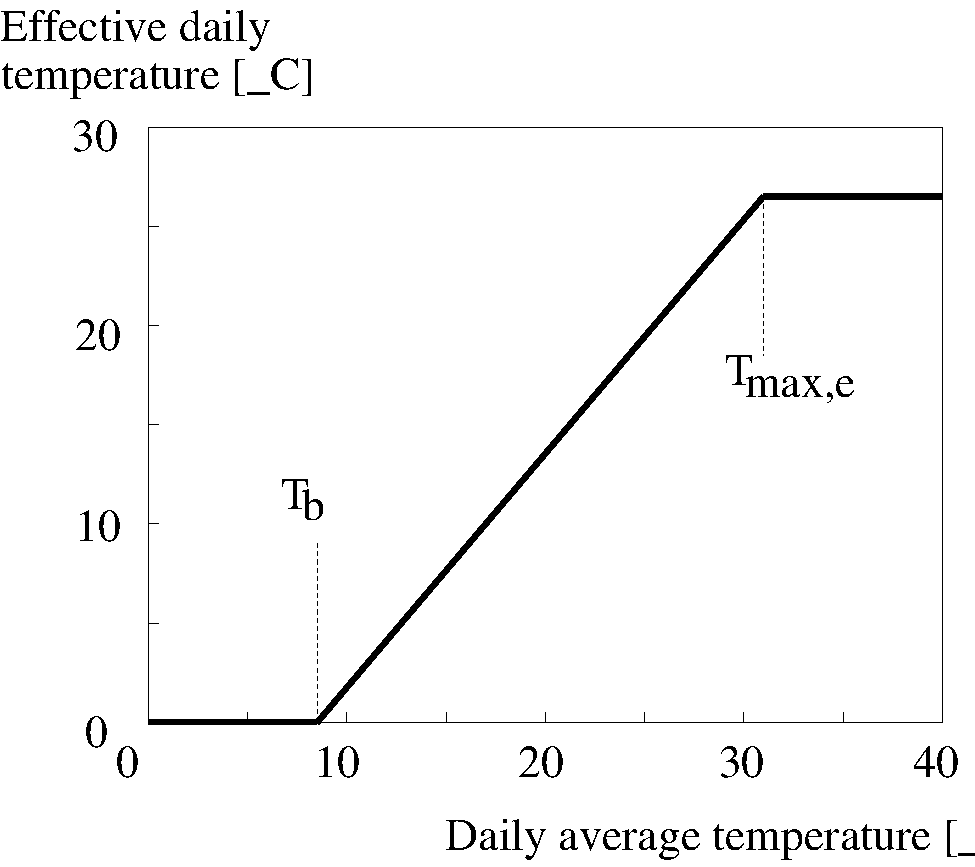
\includegraphics[width=120mm]{\FigDir/TEFFMAX.pdf}
\caption{Effective temperature from sowing to emergence} 
\label{fig:TEFFMAX}
% \begin{center}\InputPS{\FigDir/TEFFMAX.eps} \end{center}
\end{figure}

The following relationship can be defined for the effective temperature sum:

\begin{align}
T_{e} &= 0            & T \le T _{b} \nonumber  \\
T_{e} &= T~-~ T _{b}  & T _{b} ~<~T ~ < ~T _{\max ,e} \nonumber  \\
T_{e} &= T _{\max ,e} & T _{b} T \ge  T _{\max \, ,\, e}
\end{align}

Where:\\[5pt]
\begin{tabularx}{\textwidth}{llXr}
T$_{{\rm e}}$ &:& Effective daily temperature & 
    [\degrees C]\\
T$_{{\rm max,e}}$ &:& Maximum temperature beyond which phenological 
    activity does not increase    &    [\degrees C]\\
T$_{{\rm b}}$ &:& Base temperature below which phenological development stops & 
    [\degrees C]\\
T  &:& (Average) daily temperature & [\degrees C]
\end{tabularx}

The base temperature, {\bf T$_{{\rm b}}$} (acronym: {\bf TBASEM}), is defined as the lower threshold
temperature below which phenological activity stops. It is a crop specific variable and
should be provided by the user. The maximum temperature beyond which phenological
activity does not increase, {\bf T$_{{\rm max,e}}$} (acronym: {\bf TEFFMX}) is also crop specific and should be
given by the user. Species originating from temperate regions show a base temperature of
0$-$3\degrees C, while species of subtropical and tropical origins have a base temperature of
9$-$14\degrees C (Angus {\it et al.}, 1981). Within a species, cultivars may vary substantially in their
temperature requirements. The temperature sum, therefore, must be characterized for
each cultivar or group of cultivars (maturity classes).   

As mentioned earlier, the start of the growing season can be either the sowing date or the
day of emergence. If the sowing date is chosen, it should be provided by the user or it
can be calculated by the model (see Appendix 4).

\subsection{Phenological development stage}
\label{sec:DVS}

The phenological development rate and development stage are calculated in subroutine
{\bf CROPSI} or {\bf CRSIM}. A crop passes through successive phenological development stages.
The length of these stages depends on the development rate. Development rates before
and after anthesis are controlled day length and/or temperature. In the model before
anthesis, both factors, temperature and day length, can be active. After anthesis only
temperature influence is possible.
Temperature is the main environmental factor affecting the development rate. Higher
temperatures accelerate the development rate leading to shorter growing periods. This rate
responds to temperature according to a curvilinear relationship. However, it has often
been demonstrated, that over a wide range of temperatures, the development rate
increases more or less linearly with temperature (van Dobben, 1962; van Keulen \&
Seligman, 1987).

The development rate (for most crops) is expressed on a numerical scale that ranges from
0 to 2, with 0 being emergence, 1 anthesis and 2 maturity. The development rate is
defined as that part of the scale that is accumulated per day for a given variety. For
example, if the time lapse between emergence and anthesis is 50 days, the average
development rate during the pre-anthesis phase is 1/50 or 0.02 d$^{{\rm -1}}$. The development stage
can also be related to the temperature sum, expressed in degree days, that is the sum of
daily temperatures over the period emergence-anthesis or anthesis-maturity. 

The development rate per day is then the ratio of daily temperature and temperature sum
(van Heemst, 1986a; 1986b). This assumes a proportionality between temperature and
development rate. However, its validity is limited.

In the model a more flexible relation is used where the effective increase in temperature
sum, used for the calculation of the development rate, is dependent on the daily temperature 
(Summerfield \& Roberts, 1987). This relation is specified in an AFGEN table, 
allowing to account for non-linearity (lower and upper threshold values and optimum
ranges). The average temperature is the independent variable in the AFGEN table (see
Appendix 2). The development rate can thus be obtained by:

\begin{equation}
% eq 5.3
\label{eq:5.3}
D_{r,t} = {\frac{DT_{s}}{\sum T_{i}}}
\end{equation}

Where:\\[5pt]
\begin{tabularx}{\textwidth}{llXr}
D$_{{\rm r,t}}$ &:& Development rate at time step t  & [d$^{{\rm -1}}$]\\
DT$_{{\rm s}}$ &:& Temperature dependent correction factor & [\degrees C]\\
$\sum$T$_{{\rm i}}$ &:& Temperature sum required to complete stage i & [\degrees C d]\\
\end{tabularx}

The temperature dependent correction factor, {\bf DT$_{{\rm s}}$} (acronym: {\bf DTSMTB}) and 
the temperature sum required to complete stage i, {\bf $\sum$T$_{{\rm i}}$} (acronym: 
{\bf TSUM1} or {\bf TSUM2}) are crop dependent and should be provided by the user.

The development stage at time step t is the integral of the development rate over the time
(i.e. time span from emergence to current time step) and can be calculated according to:

\begin{equation}
\label{eq:5.4}
D_{s,t} ~=~ D_{s,t-1} + D_{r,t} \Delta t
\end{equation}

Where:\\[5pt]
\begin{tabularx}{\textwidth}{llXr}
D$_{{\rm s,t}}$ &:& Development stage at time step t    &    [-]\\
D$_{{\rm r,t}}$ &:& Development rate at time step t     &   [d$^{{\rm -1}}$]\\
$\Delta$t &:& Time step   &     [d]\\
\end{tabularx}

For certain species or cultivars, during the vegetative stage (i.e. D$_{{\rm s}}$ $<$ 1), the 
effect of day length should be taken into account. Approaches that describe such effects 
quantitatively are given amongst others by  Weir {\it et al.} (1984), Hadley {\it et al}. (1984) 
and Reinink {\it et al.} (1986). In the model, a reduction factor for the development rate as a 
function of the day length is introduced. In case of photosensitivity, this reduction factor 
should be multiplied with equation \ref{eq:5.3} and can be calculated as:

\begin{equation}
\label{eq:5.5}
f_{red} ~=~{\frac{D ~-~D _{c} }{D _{o} ~-~ D _{c} }} ~~~~~~~~~0~\le ~f _{red} ~\le ~1
\end{equation}

Where:\\[5pt]
\begin{tabularx}{\textwidth}{llXr}
f$_{{\rm red}}$ &:& Development rate reduction factor as function of day length   &     [-]\\
D &:& Present day length (see eq. \ref{eq:AstroDaylength})   &     [h]\\
D$_{{\rm c}}$ &:& Critical day length for development (lower threshold)    &    [h]\\
D$_{{\rm o}}$ &:& Optimum day length for development (upper threshold)    &    [h]\\
\end{tabularx}

The user should provide information whether the development rate depends on temperature, 
on day length or on temperature and day length (acronym: {\bf IDSL}). The critical
daylength, {\bf D$_{{\rm c}}$} (acronym: {\bf DLC}) and the optimum daylength, 
{\bf D$_{{\rm o}}$} (acronym: {\bf DLO}) are crop dependent and should also be provided by 
the user. 

Note that in modern cultivars, photosensitivity is much less pronounced than in traditional
cultivars, and that for the purpose of modelling the day length influence can be ignored
by choosing an appropriate temperature sum, which lead to  an equivalent crop life cycle.

The simulation of crop growth stops when the development stage reaches the stage at
which the crop will be harvested (acronym: {\bf DVSEND}). This development stage should be
provided by the user. 

\section{Daily assimilation  } 

Daily dry matter production is the most detailed part of the model. The following steps
can be distinguished and will be described separately:
\begin{itemize}
\item Total daily gross CO2 assimilation rate of the canopy 
    [\S \ref{sec:DailyGrossAssimilation}]
\item Total instantaneous gross CO$_{{\rm 2}}$ assimilation of the canopy 
    [\S \ref{sec:InstantGrossAssimilation}]
\end{itemize}
 
The daily rate of CO$_{{\rm 2}}$ assimilation of the crop is driven by the intercepted light and can
be obtained by integrating the total instantaneous CO$_{{\rm 2}}$ assimilation rate of the canopy over
the day. The total instantaneous assimilation rate is calculated in subroutine {\bf ASSIM}, the
integration of the total instantaneous assimilation rate in subroutine {\bf TOTASS}. Both
calculations make use of the Gaussian integration method (Scheid, 1968), a simple and
fast method of numerical integration. This integration method is explained in Appendix 1.
For calculating daily total assimilation, this 3-point integration method performs very well
(Goudriaan, 1986; Spitters, 1986)

\subsection{Total daily gross CO2 assimilation rate of the canopy}
\label{sec:DailyGrossAssimilation}

To calculate the total daily gross CO$_{{\rm 2}}$ assimilation rate of the whole canopy, an integration over time should be performed. Therefore, for given fluxes of photosynthetically
active radiation, at three different periods of the day, the total instantaneous gross canopy
CO$_{{\rm 2}}$ assimilation rate is computed. Afterwards, the integral of the total instantaneous
gross canopy CO$_{{\rm 2}}$ assimilation rate over time, as a weighted average of the selected three
hours, is calculated (Gaussian integration, see Appendix 1).

For the calculation of the total instantaneous gross canopy CO$_{{\rm 2}}$ assimilation rate, an
integration over depth of the gross instantaneous assimilation rate has to be performed.
Therefore, at three different depths in the canopy the gross instantaneous assimilation rate
is calculated, whereafter the integral of the gross instantaneous assimilation rate over
depth, as a weighted average of the selected depths, is computed (Gaussian integration,
see Appendix 1)

Integration, to calculate the daily total assimilation, is only necessary if instantaneous
assimilation will take place. Instantaneous assimilation will be zero if the leaf area index
equals zero (no photosynthetic activity). A second restriction for the integration is the
maximum CO$_{{\rm 2}}$ assimilation rate as a function of development stage, which is crop
dependent. When this maximum assimilation rate at light saturation equals zero also no
instantaneous assimilation will take place and no integration has to be performed.

As is mentioned before, in order to integrate the gross instantaneous assimilation rate
over the day, three points in time are selected to calculate the photosynthetically active
radiation. In this particular case, the radiation is homogeneously distributed over the day
according to the sine of the solar elevation, so the weighted average CO$_{{\rm 2}}$ 
assimilation rate can therefore be calculated for half a day only.

The three points in time are selected from noon to sunset (this explains the use of the
constants 0.5 and 12.00):

\begin{equation}
% eq 5.6
t_{h} = 12 + 0.5 \cdot D \cdot (0.5 ~+~ p\, \sqrt{0.15}) ~~~ for ~~~ p = -1,0,1
\end{equation}

Where:\\[5pt]
\begin{tabularx}{\textwidth}{llXr}
D &:& Day length (see eq. 4.25)    &    [h]\\
t$_{{\rm h}}$ &:& Hour of the day  &      [h]\\
p &:& Gaussian integration points  &      [-]\\
\end{tabularx}

The incoming radiation and therefore gross assimilation rate, changes with solar elevation. 
The solar height as a function of the hour of the day can be calculated with:

\begin{equation}
\label{eq:5.7}
\sin \beta ~=~ \sin \lambda \, \sin \sigma ~+~ \cos \lambda \, \cos \sigma \, \cos \, 
(\, 2 \pi \,{\frac{t _{h} ~+~ 12}{24}} )
\end{equation}


Where:\\[5pt]
\begin{tabularx}{\textwidth}{llXr}
$\beta$ &:& Solar elevation   &    [degrees]\\
$\sigma$ &:& Solar declination    &    [degrees]\\
$\lambda$ &:& Latitude     &   [degrees]\\
t$_{{\rm h}}$ &:& Hour of the day    &    [h]\\
\end{tabularx}

Measured or estimated daily global solar radiation  (wavelength 300 - 3000 nm) is input
in the model. Only half of this incoming radiation is photosynthetically active (PAR,
Photosynthetically Active Radiation, wavelength 400 - 700 nm). This fraction, which is
generally called 'light' or 'visible radiation', is used in the calculation procedure of the
CO$_{{\rm 2}}$ assimilation rate of the canopy. In the model, the instantaneous incoming 
photosynthetically active radiation is calculated by multiplying half of the daily global radiation
with the ratio of the actual effective solar elevation and the integral of the effective solar
height (see also eq. \ref{eq:IntSolarHeight}):

\begin{equation}
\label{eq:5.8}
I _{0} ~=~ 0.5\, S _{g,d} \,{\frac{\sin \beta \, (\, 1~+~0.4\, \sin \beta \, )}{\int \, \sin \beta _{m} }}
\end{equation}

Where:\\[5pt]
\begin{tabularx}{\textwidth}{llXr}
I$_{{\rm 0}}$ &:& Photosynthetically active radiation flux    &    
    [J m$^{{\rm -2}}$ s$^{{\rm -1}}$]\\
S$_{{\rm g,d}}$ &:& Daily global radiation   &     
    [J m$^{{\rm -2}}$ d$^{{\rm -1}}$] \\
$\beta$ &:& Solar elevation    &    [degrees]\\
$\int \sin \beta_{{\rm m}}$ &:& The corrected integral of solar height over the day 
    for non homogeneous atmospheric transmission (eq. \ref{eq:IntSolarHeight})   
    &     [s]\\
\end{tabularx}

The calculated photosynthetically active radiation flux consists of a diffuse flux and a
direct flux. The diffuse flux is the result of scattering of sun rays by clouds, aerosols and
gases in the atmosphere. The proportion of diffuse light in the total incident light flux
depends on the status of the atmosphere (see also eq. \ref{eq:irrad_diffuse}). This fraction 
is calculated from the atmospheric transmission using an empirical function (Spitters 
{\it et al.}, 1986).

\begin{equation}
% eq 5.9
I_{0,df} ~=~ D _{p~} \sin \beta
\end{equation}

Where:\\[5pt]
\begin{tabularx}{\textwidth}{llXr}
I$_{{\rm 0,df}}$ &:& Diffuse part of the photosynthetically active radiation flux 
   at top of the canopy    &    [J m$^{{\rm -2}}$ s$^{{\rm -1}}$]\\
D$_{{\rm p}}$ &:& Diffuse radiation perpendicular to the direction 
   light (see eq. 4.31)    &    [J m$^{{\rm -2}}$ s$^{{\rm -1}}$]\\
sin$\beta$ &:& Solar elevation (see eq. \ref{eq:5.7})    &    [degrees]\\
\end{tabularx}

The direct part can be easily obtained by subtracting the diffuse part from the
photosynthetically radiation flux:

\begin{equation}
% eq 5.10
I_{0,dr} ~=~ I_{0} ~-~I_{0,df} 
\end{equation}
 
Where:\\[5pt]
\begin{tabularx}{\textwidth}{llXr}
I$_{{\rm 0,dr}}$ &:& Direct part of the photosynthetically active radiation flux 
   at top of the canopy    &    [J m$^{{\rm -2}}$ s$^{{\rm -1}}$]\\
I$_{{\rm 0}}$ &:& Photosynthetically active radiation flux (see eq. \ref{eq:5.8})    &  
   [J m$^{{\rm -2}}$ s$^{{\rm -1}}$]\\
I$_{{\rm 0,df}}$ &:& Diffuse part of the photosynthetically active radiation flux 
   at top of the canopy     &   [J m$^{{\rm -2}}$ s$^{{\rm -1}}$]\\
\end{tabularx}

Once the photosynthetically active radiation fluxes have been established, the 
instantaneous gross assimilation rate of the canopy can be calculated (see \S
 \ref{sec:InstantGrossAssimilation}). And the integration over time can take place.
The integral of the total gross canopy assimilation rate over time is calculated as the
weighted average of the three selected hours of the day. Multiplying by the day length
results in the total daily gross rate of CO$_{{\rm 2}}$ assimilation. 

\begin{equation}
\label{eq:5.11}
A_{d} = D {\frac{A_{C,-1} ~+~ 1.6 A_{C,0} ~+~ A_{C,1} }{3.6}}
\end{equation}

Where:\\[5pt]
\begin{tabularx}{\textwidth}{llXr}
A$_{{\rm d}}$ &:& Total gross assimilation rate    &    
[kg ha$^{{\rm -1}}$ d$^{{\rm -1}}$]\\
D &:& Day length (see eq. \ref{eq:AstroDaylength})   &     [h]\\
A$_{{\rm C}}$ &:& Total inst. gross assimilation rate for
   the whole canopy, p= -1,0,1 (see eq. \ref{eq:5.31})    &
   [kg ha$^{{\rm -1}}$ h$^{{\rm -1}}$]\\
\end{tabularx}

\subsection{Total instantaneous gross CO$_{2}$ assimilation of the canopy}  
\label{sec:InstantGrossAssimilation}

In the subroutine {\bf ASSIM}, the total instantaneous rate of CO$_{{\rm 2}}$ assimilation of the canopy is
calculated from the incoming fluxes of diffuse and direct photosynthetic active radiation,
solar elevation and leaf area index and several parameters.

\subsubsection{Reflection and extinction}
The total incoming photosynthetically active radiation flux is partly reflected by the
canopy. The reflection coefficient is defined as the fraction of the downward radiation
flux that is reflected by the whole canopy. According to Goudriaan (1977), the reflection
coefficient of a green leaf canopy with a random spherical leaf angle equals:

\begin{equation}
\label{eq:5.12}
\rho = {\frac{1- \sqrt{1-\sigma}}{1 + \sqrt{1-\sigma}}} \cdot {\frac{2}{1+1.6 \sin \beta }}
\end{equation}

Where:\\[5pt]
\begin{tabularx}{\textwidth}{llXr}
$\rho$ &:& Reflection coefficient of a green leaf canopy    &    [-]\\
$\sigma$ &:& Scattering coefficient fraction (transmission and reflection) 
   of single leaves for visible radiation   
   {\small (=0.2; Goudriaan, cited by Spitters, 1986)}  &     [-]\\  
$\beta$ &:& Solar elevation (see eq. \ref{eq:SolarElevation})    &    [degrees]\\
\end{tabularx}
 
The first term denotes the reflection of the canopy of horizontal leaves and the second
term is the approximate correction factor for a spherical leaf angle distribution.

A fraction (1-$\rho$) of the incoming visible radiation is potentially available for absorption by
the canopy. Radiation fluxes attenuate exponentially within a canopy with increasing leaf
area from the top downwards:

\begin{equation}
\label{eq:5.13}
I_{L~} = I_{0} (1~-~\rho ) e^{-\kappa LAI_{L} }
\end{equation}

Where:\\[5pt]
\begin{tabularx}{\textwidth}{llXr}
I$_{{\rm L}}$   &:& Net photosynthetic active radiation flux at 
    depth L in the canopy    &    [J m$^{{\rm -2}}$ s$^{{\rm -1}}$]\\
I$_{{\rm 0}}$   &:& Photosynthetically active radiation flux (see eq. \ref{eq:5.8})  & 
    [J m$^{{\rm -2}}$ s$^{{\rm -1}}$]\\
LAI$_{{\rm L}}$ &:& Cumulative leaf area index (from top downwards) 
    relative depth L & [ha ha$^{{\rm -1}}$]\\
$\rho$          &:& Reflection coefficient of the canopy   &     [-]\\
$\kappa$        &:& Extinction coefficient for photosynthetic active 
    radiation flux   &     [-]\\
\end{tabularx}

The diffuse and the direct flux have different extinction coefficients, giving rise to
different light profiles within the canopy for diffuse and direct radiation. Therefore three
different radiation fluxes are distinguished:
\begin{itemize}
\item the diffuse flux, with extinction coefficient $\kappa_{df}$;
\item the total direct flux, with extinction coefficient $\kappa_{dr,t}$;
\item the direct component of direct light, with extinction coefficient $\kappa_{dr,bl}$.
\end{itemize}

Radiation becomes diffuse when sun rays are partly absorbed and partly scattered (i.e.
reflected or transmitted) by a leaf. The subscript {\it bl} (black) is used, the leaves show
neither transmission nor reflection. The extinction coefficient of 'black leaves'
can be calculated as:

\begin{equation}
% eq 5.14
\label{eq:5.14}
\kappa_{bl} ~=~{\frac{0.5}{\sin \beta }}
\end{equation}

Where:\\[5pt]
\begin{tabularx}{\textwidth}{llXr}
$\kappa$$_{{\rm bl}}$ &:& Extinction coefficient for the direct radiation flux   &     [-]\\
$\beta$ &:& Solar elevation    &    [degree]\\
\end{tabularx}

For a spherical leaf area distribution (homogeneous, random), the extinction coefficient
for the diffuse radiation flux equals:

\begin{equation}
\label{eq:5.15}
 \kappa_{df} ~=~ \kappa_{bl} \, \sqrt{1~-~ \sigma }
\end{equation}

Where:\\[5pt]
\begin{tabularx}{\textwidth}{llXr}
$\kappa$$_{{\rm df}}$ &:& Extinction coefficient for the diffuse radiation flux    &    [-]\\
$\sigma$ &:& Scattering coefficient fraction of single leaves for 
   visible radiation    &    [-]\\
\end{tabularx}

In the model, the extinction coefficient for the diffuse radiation flux, 
{\bf $\kappa$$_{{\rm df}}$} (acronym: {\bf KDIF})
is not computed but should be provided by the user. It can be measured directly 
under diffuse sky conditions.

In equation \ref{eq:5.14}, 0.5 points to the average projection on the ground surface of leaves
showing a spherical angle distribution, and 0.8 in equation \ref{eq:5.16} is the value of 0.5/sin$\beta$
averaged over elevation $\beta$ of incident radiation under an overcast sky.

The average extinction coefficient for the diffuse radiation flux is about 0.72 (Goudriaan,
1977). However, in many situations, the leaf angle distribution is not spherical. For
example in rice, the leaves are clustered (especially in the beginning as a result of
planting on hills), and have a very vertical orientation. Other leaf angle distributions can
be accounted for by a procedure described by Goudriaan (1986), which calculates the
extinction coefficient for the diffuse radiation flux on the basis of the frequency 
distribution of leaves with angles in different classes.

In the model however, the leaf angle distribution is accounted for by using a so called
cluster factor which is the measured extinction coefficient for diffuse radiation flux,
relative to the theoretical one for a spherical leaf area distribution. The cluster factor can
be calculated as: 

\begin{equation}
\label{eq:5.16}
C _{f} ~=~{\frac{ \kappa _{df} }{0.8\, \sqrt{1 ~-~ \sigma } }}
\end{equation}

Where:\\[5pt]
\begin{tabularx}{\textwidth}{llXr}
C$_{{\rm f}}$ &:& Cluster factor    &    [-]\\
$\kappa$$_{{\rm df}}$ &:& Extinction coefficient for diffuse radiation flux   &     [-]\\
$\sigma$ &:& Scattering coefficient fraction of single leaves for
   visible radiation  &      [-]\\
\end{tabularx}

The direct component can be calculated as (Goudriaan, 1977):

\begin{equation}
\label{eq:5.17}
\kappa _{dr,bl} ~=~{ C _{f} }\,{\frac{0.5}{\sin \beta }}
\end{equation}

Where:\\[5pt]
\begin{tabularx}{\textwidth}{llXr}
$\kappa$$_{{\rm dr,bl}}$ &:& Extinction coefficient for the direct component of direct light   &     [-] \\
C$_{{\rm f}}$ &:& Cluster factor     &   [-]\\
$\beta$ &:& Solar elevation     &   [degrees]\\
\end{tabularx}

The extinction coefficient for the total direct radiation flux can be calculated as (Goudriaan, 1977):

\begin{equation}
\label{eq:5.18}
\kappa _{dr,t} ~=~ \kappa _{dr,bl} \sqrt{1~-~\sigma }
\end{equation}

Where:\\[5pt]
\begin{tabularx}{\textwidth}{llXr}
$\kappa_{dr,t}$ &:& Extinction coefficient for total direct radiation flux   &    [-]\\
$\kappa_{dr,bl}$ &:& Extinction coefficient for the direct component of direct light  &   [-]\\
$\sigma$ &:& Scattering coefficient     &    [-]\\
\end{tabularx}

\subsubsection{Absorption}
Three depths in the canopy are selected according to the Gaussian integration method (see
Appendix 1) and at those levels the leaf area index, the amount of absorbed radiation and
the leaf CO$_{{\rm 2}}$ assimilation is calculated. The total instantaneous assimilation is easily
obtained by multiplying the instantaneous assimilation with the total leaf area index (eq.
\ref{eq:5.31}). In the following text the calculation processes, concerning the instantaneous
assimilation, will be explained in detail. Calculation of the leaf area index will be
explained in \S \ref{sec:5.4.5}.

Canopy assimilation is calculated as a weighted average of the assimilation at three
horizons within the canopy. The leaf area index of the selected horizons can be written as
(Goudriaan, 1986):

\begin{equation}
% eq 5.19 a-d
LAI_{L} = (0.5 + p \sqrt{0.15}) \cdot LAI~~~~for~~~~p = -1,0,1
\end{equation}

 
Where:\\[5pt]
\begin{tabularx}{\textwidth}{llXr}
LAI$_{{\rm L}}$ &:& Leaf area index at relative distance L in the canopy 
    (L=0 at the top)    &    [ha ha$^{{\rm -1}}$]\\
\end{tabularx}

The light absorbed at a certain depth in the canopy is obtained by taking the derivative of
equation \ref{eq:5.13} with respect to the cumulative leaf area index:

\begin{equation}
% eq 5.20
I_{a,L} = {\frac{-dI _{0\, ,\, L} }{dL}} = \kappa (1 -  \rho) I_{0} \cdot e^{- \kappa LAI_{L}}
\end{equation}

Where:\\[5pt]
\begin{tabularx}{\textwidth}{llXr}
I$_{{\rm a,L}}$ &:& Amount absorbed of total radiation flux
    \footnote{With the 'Total radiation flux' in this paragraph the total photosynthetically 
        active radiation flux is meant.} at relative depth L    &    
    [J m$^{{\rm -2}}$ s$^{{\rm -1}}$]\\
I$_{{\rm 0,L}}$ &:& Net photosynthetic active radiation at relative depth L in 
    the canopy    &    [J m$^{{\rm -2}}$ s$^{{\rm -1}}$]\\
I$_{{\rm 0}}$ &:& Photosynthetically active radiation flux at top of the 
    canopy   &     [J m$^{{\rm -2}}$ s$^{{\rm -1}}$]\\
L &:& Relative depth in the canopy   &     [-]\\
$\kappa$ &:& The extinction coefficient for the PAR flux    &     [-]\\
$\rho$ &:& Reflection coefficient of the canopy (see eq. \ref{eq:5.12})   &     [-]\\
\end{tabularx}

If expressed for the different light components, the absorbed fluxes for the different
components per unit leaf area at a certain depth in the canopy are:

\stepcounter{equation}
\begin{align}
% equation 5.21a-c
I_{a,df} &={\frac{-dI_{df,L}}{dL}} &
         &= \kappa_{df} (1 - \rho)\, I_{0,df} \cdot e^{-\kappa_{df} \, LAI_{L}} \subeqn  \\
I_{a,dr,t} &= {\frac{-dI_{dr,t,L}}{dL}} & 
           &= \kappa_{dr,t} (1-\rho) I_{0,dr} \cdot e^{-\kappa_{dr,t} LAI_{L}} \subeqn  \\
% TODO: check if below I_{a,dr,dr} should be changed to I_{a,dr,bl}
I_{a,dr,dr} &= {\frac{-dI_{dr,L}}{dL}} &
            &= \kappa_{dr,bl} (1-\sigma) I_{0,dr} \cdot e^{-\kappa_{dr,bl} LAI_{L}} \subeqn
\end{align}

Where:\\[5pt]
\begin{tabularx}{\textwidth}{llXr}
I$_{{\rm a,.}}$ &:& Amount absorbed of specified radiation flux   &      
    [J m$^{{\rm -2}}$ s$^{{\rm -1}}$]\\
I$_{{\rm .,L}}$ &:& Net specified component of PAR flux at relative depth L    &    
    [J m$^{{\rm -2}}$ s$^{{\rm -1}}$]\\
I$_{{\rm 0}}$ &:& Photosynthetically active radiation flux at top of the canopy
    (see eq. \ref{eq:5.8})   &   [J m$^{{\rm -2}}$ s$^{{\rm -1}}$]\\
L &:& Relative depth in the canopy   &     [-]\\
$\kappa$$_{{\rm .}}$ &:& The extinction coefficient for specified radiation 
    (see eq. \ref{eq:5.15}, \ref{eq:5.17} and \ref{eq:5.18})    &    [-]\\
$\rho$ &:& Reflection coefficient of the canopy (see eq. \ref{eq:5.12})   &     [-]\\
$\sigma$ &:& Scattering coefficient    &    [-]\\
bl &:& Black &\\
df &:& Diffuse &\\
dr &:& Direct &\\
t &:& Total &\\
\end{tabularx}

Note that of the direct component of the direct flux the non-scattered part (1-$\sigma$) is
absorbed.

The total absorbed flux for shaded leaves can be calculated as the sum of the absorbed
flux of diffuse radiation and absorbed flux of the diffuse radiation of the indirect
component of direct radiation. The last one is equal to the difference of the absorbed flux
of the total radiation minus the absorbed flux of the direct component of the direct
radiation.

\begin{equation}
\label{eq:5.22}
I _{a,sh} ~=~ I _{a,df} ~+~ (I_{a,dr,t} ~-~ I_{a,dr,dr} )
\end{equation}

Where:\\[5pt]
\begin{tabularx}{\textwidth}{llXr}
I$_{{\rm a,sh}}$ &:& Absorbed amount of the total radiation flux by shaded leaves
    &    [J m$^{{\rm -2}}$ s$^{{\rm -1}}$]\\
I$_{{\rm a,df}}$ &:& Absorbed amount of the diffuse radiation flux
   &     [J m$^{{\rm -2}}$ s$^{{\rm -1}}$]\\
I$_{{\rm a,dr,t}}$ &:& Absorbed amount of the total direct radiation flux
   &     [J m$^{{\rm -2}}$ s$^{{\rm -1}}$]\\
I$_{{\rm a,dr,dr}}$ &:& Absorbed amount of direct component of the  direct radiation flux
   & [J m$^{{\rm -2}}$ s$^{{\rm -1}}$]\\
\end{tabularx}


\subsubsection{Instantaneous gross assimilation}
The CO$_{{\rm 2}}$ assimilation-light response can be obtained by introducing the absorbed amount
of light into an assimilation-light response function of individual leaves. Satisfactory
results can be acquired with (Peat, 1970):

\begin{equation}
\label{eq:5.23}
A_{L} = A_{m} (1-\exp({{-\epsilon I_{a}}/{A_{m}}}))
\end{equation}

Where:\\[5pt]
\begin{tabularx}{\textwidth}{llXr}
A$_{{\rm L}}$ &:& Inst.\footnote{ Inst. = Instantaneous} gross assimilation 
     rate at relative depth L (per unit leaf area)    &    
     [kg ha$^{{\rm -1}}$ h$^{{\rm -1}}$]\\
A$_{{\rm m}}$ &:& Inst. gross assimilation rate at light saturation    & 
     [kg ha$^{{\rm -1}}$ h$^{{\rm -1}}$]\\
$\epsilon$ &:& Initial light use efficiency   &   [(kg ha$^{{\rm -1}}$ 
     h$^{{\rm -1}}$)/(J m$^{{\rm -2}}$ s$^{{\rm -1}}$])\\
I$_{{\rm a}}$ &:& Absorbed amount of the total radiation flux     &   
     [J m$^{{\rm -2}}$ s$^{{\rm -1}}$]\\
\end{tabularx}

The instantaneous gross assimilation rate at light saturation, {\bf A$_{{\rm m}}$} (acronym: {\bf AMAXTB}) is
crop specific and should be provided by the user. It is a function of the development
stage. An AFGEN table with the development stage as the independent variable is used to
describe this dependency (see also Appendix 2). The initial light use efficiency, {\bf $\epsilon$}
(acronym: {\bf EFF}), is also crop dependent and should be provided by the user. It is
assumed, that the initial light use efficiency is always higher than 2.0 [kg ha$^{{\rm -1}}$ 
leaf h$^{{\rm -1}}$]. 

Introducing the absorbed amount of radiation by shaded leaves (eq. \ref{eq:5.22}) into 
equation \ref{eq:5.23} yields:

\begin{equation}
\label{eq:5.24}
A_{sh} = A_{m} \big(1-\exp({{-\epsilon I_{a,sh} }/{A_m}} ) \big)
\end{equation}

Where:\\[5pt]
\begin{tabularx}{\textwidth}{llXr}
A$_{{\rm sh}}$ &:& Inst. gross assimilation rate for shaded leaves  & 
    [kg ha$^{{\rm -1}}$ h$^{{\rm -1}}$]\\
A$_{{\rm m}}$ &:& Inst. gross assimilation rate at light saturation & 
    [kg ha$^{{\rm -1}}$ h$^{{\rm -1}}$]\\
$\epsilon$ &:& Initial light use efficiency  &  
    [(kg ha$^{{\rm -1}}$ h$^{{\rm -1}}$)/(J m$^{{\rm -2}}$ s$^{{\rm -1}}$)]\\
I$_{{\rm a,sh}}$ &:& Absorbed amount of the total radiation flux  by shaded leaves (see eq. \ref{eq:5.22})   &
     [J m$^{{\rm -2}}$ s$^{{\rm -1}}$]\\
\end{tabularx}

For the sunlit leaf area, the average absorption intensity may be substituted in equation
\ref{eq:5.23}. However, it is more accurate to account for the variation in leaf angle and thus in
illumination intensity (Spitters, 1986). The direct flux is absorbed by a leaf perpendicular
to the direct beam with an intensity of: 

\begin{equation}
\label{eq:5.25}
I_{a,dr,sl} = {\frac{(1-\sigma) I_{0,dr}}{\sin \beta }}
\end{equation}

Where:\\[5pt]
\begin{tabularx}{\textwidth}{llXr}
I$_{{\rm a,dr,sl}}$ &:& Absorbed amount of the direct radiation flux by leaves
   perpendicular to the direct beam    &    [J m$^{{\rm -2}}$ s$^{{\rm -1}}$]\\
I$_{{\rm 0,dr}}$ &:& Direct flux of visible radiation at the top of 
   the canopy &  [J m$^{{\rm -2}}$ s$^{{\rm -1}}$]\\
$\sigma$ &:& Scattering coefficient  &[-]\\
$\beta$ &:& Solar elevation   & [degrees]\\
\end{tabularx}

The amount of absorbed direct radiation by leaves (eq. \ref{eq:5.25}) depends on the sine of
incidence at the leaf surfaces. Therefore, for sunlit leaves, CO$_{{\rm 2}}$ assimilation rates have to
be calculated separately for leaves with different angles and integrated over the sine of
incidence. In the model a spherical leaf angle distribution is assumed, so no integration
over leaf angles is needed.

Integration over the sine of incidence for the sunlit leaves yields (Goudriaan, personal
communication):

\begin{equation}
% eq 5.26
A_{sl} = A_{m} \bigg( 
   1-(A_{m} - A_{sh})  {\frac{1~- \exp({{-I _{a,dr,sl} \, \epsilon}}/{A_m}) }
                             {\epsilon\, I _{a,dr,sl} }}
   \bigg)
\end{equation}

Where:\\[5pt]
\begin{tabularx}{\textwidth}{llXr}
A$_{{\rm sl}}$ &:& Inst. gross assimilation rate for sunlit leaves  &
    [kg ha$^{{\rm -1}}$ h$^{{\rm -1}}$]\\
A$_{{\rm sh}}$ &:& Inst. gross assimilation rate for shaded leaves  &
    [kg ha$^{{\rm -1}}$ h$^{{\rm -1}}$]\\
A$_{{\rm m}}$ &:& Inst. gross assimilation rate at light saturation &
    [kg ha$^{{\rm -1}}$ h$^{{\rm -1}}$]\\
I$_{{\rm a,dr,sl}}$ &:& Absorbed amount of the direct radiation flux by leaves
    perpendicular to the direct beam  &  [J m$^{{\rm -2}}$ s$^{{\rm -1}}$]\\
$\epsilon$ &:& Initial light use efficiency  &   [(kg ha$^{{\rm -1}}$ 
    h$^{{\rm -1}}$)/(J m$^{{\rm -2}}$ s$^{{\rm -1}}$)]\\
\end{tabularx}

The assimilation rate per unit leaf area at a specific depth in the canopy is the sum of the
assimilation rates of sunlit and shaded leaves, taking into account the proportion of sunlit
and shaded leaf area at that depth in the canopy. 

The fraction sunlit leaf area equals the fraction of the direct radiation reaching that layer:

\begin{equation}
% eq 5.27
f_{sl} =  e^{-\kappa_{dr,bl} \cdot LAI_{L}}
\end{equation}
 
Where:\\[5pt]
\begin{tabularx}{\textwidth}{llXr}
f$_{{\rm sl}}$ &:& Fraction sunlit leaf area   &     [-]\\
$\kappa$$_{{\rm dr,bl}}$ &:& Extinction coefficient for the direct component of
   direct radiation (see eq. \ref{eq:5.17})   &     [-]\\
LAI$_{{\rm L}}$ &:& Cumulative leaf area index at relative depth L in canopy  &      [-]
\end{tabularx}

The total instantaneous assimilation rate at a relative depth L can be calculated as:

\begin{equation}
\label{eq:5.28}
A_{T,L} = f_{sl} A_{sl} + (1 - f_{sl}) A_{sh} 
\end{equation}

Where:\\[5pt]
\begin{tabularx}{\textwidth}{llXr}
A$_{{\rm T,L}}$ &:& Total inst. gross assimilation rate at a relative depth L   &
     [kg ha$^{{\rm -1}}$ h$^{{\rm -1}}$]\\
A$_{{\rm sl}}$ &:& Inst. gross assimilation rate for sunlit leaves  & 
     [kg ha$^{{\rm -1}}$ h$^{{\rm -1}}$]\\
A$_{{\rm sh}}$ &:& Inst. gross assimilation rate for shaded leaves  & 
     [kg ha$^{{\rm -1}}$ h$^{{\rm -1}}$]\\
f$_{{\rm sl}}$ &:& Fraction sunlit leaf area  &  [-]\\
\end{tabularx}

The total instantaneous assimilation rate for the whole canopy per unit leaf area can be
established using the Gaussian integration method, as a weighted average of the assimilation 
at three levels within the canopy.
However, first the leaf area index of the levels selected have to be established:

\begin{equation}
\label{eq:5.29}
LAI_{L} = (0.5+p \sqrt{0.15})LAI~~~~for~~~~p=-1,0,1
\end{equation}

Where:\\[5pt]
\begin{tabularx}{\textwidth}{llXr}
LAI$_{{\rm L}}$ &:& Leaf area index at relative depth L in canopy    &    [ha ha$^{{\rm -1}}$]\\
LAI &:& Total leaf area of the crop (see \S \ref{sec:5.4.5}) &   [ha ha$^{{\rm -1}}$]\\
\end{tabularx}

Introducing the values of the leaf area index of the three selected layers in the equations
mentioned before, will yield the instantaneous assimilation at these horizons. The
weighted average of these values yields the total instantaneous assimilation rate for the
whole canopy per unit leaf area.

The weighted average of the total instantaneous assimilation rates can be calculated as:

\begin{equation}
% eq 5.30
A_{C,l} = {\frac{(A_{T,L,-1} + 1.6 A_{T,L,0} + A_{T,L,1})}{3.6}}
\end{equation}

Where:\\[5pt]
\begin{tabularx}{\textwidth}{llXr}
A$_{{\rm C,l}}$ &:& Total instantaneous canopy assimilation 
   rate (per unit leaf area)    &    [kg ha$^{{\rm -1}}$ h$^{{\rm -1}}$]\\
A$_{{\rm T,L,p}}$ &:& Total instantaneous gross assimilation rate at relative 
   depth L (see eq. \ref{eq:5.28}) at p= -1,0,1 (see eq. \ref{eq:5.29})    &    
   [kg ha$^{{\rm -1}}$ h$^{{\rm -1}}$]\\
\end{tabularx}

This total instantaneous assimilation rate is calculated per unit leaf area and must
therefore be multiplied with the leaf area index to yield the total assimilation rate for the
whole canopy:

\begin{equation}
\label{eq:5.31}
A_{C} = A_{C,l} \cdot LAI
\end{equation}

Where:\\[5pt]
\begin{tabularx}{\textwidth}{llXr}
A$_{{\rm C}}$ &:& Total inst. gross assimilation rate for
   the whole canopy  &  [kg ha$^{{\rm -1}}$ h$^{{\rm -1}}$]\\
A$_{{\rm C,l}}$ &:& Total inst. gross canopy assimilation rate 
   per unit leaf area &  [kg ha$^{{\rm -1}}$ h$^{{\rm -1}}$]\\
LAI &:& Total leaf area of the crop (see \S \ref{sec:5.4.5})  & [ha ha$^{{\rm -1}}$]\\
\end{tabularx}

Note that the green parts of the stems and the storage organs (like panicles) may absorb a
substantial amount of radiation. Therefore, the green area index of these organs is added
to the total leaf area. The green area index of the stems and storage organs can be
calculated by multiplying the dry weight of the organ with respectively the specific stem
area and the specific pod area (see also \S \ref{sec:5.4.5} and eq. \ref{eq:5.24}). The specific 
stem area and specific pod area are crop specific and should be provided by the user.


\section{Crop growth}

The gross CO$_{{\rm 2}}$ assimilation discussed in chapter 5.3 is the basis for crop growth. The
resulting actual crop growth depends further on a number of assimilation reducing factors
and assimilation requirements for maintenance respiration and bio-synthesis i.e. the
conversion of primary assimilates into plant tissue. The remaining dry matter is partioned
over the various organs. Besides growth, there may be death of the plant organs. All
these processes simulated in {\bf CROPSI} or {\bf CRSIM} are described in the following sections.

\subsection{Actual gross photosynthesis}

In chapter 5.3, the assimilation was treated as a function of the intercepted light and of
photosynthetic crop characteristics such as initial light use efficiency and maximum leaf
CO$_{{\rm 2}}$ assimilation at light saturation. The value of some crop characteristics are dependent
on phenological crop stage. In addition, the assimilation process can be hampered by
suboptimum temperatures and/or by reduced availability of CO$_{{\rm 2}}$ due to closure of the leaf
stomata as means to reduce transpiration. Thus, the gross assimilation depends on
development stage, on temperature and on the transpiration rate. In this paragraph this
dependency will be briefly explained.

\subsubsection{Development stage}
As mentioned before, the instantaneous gross assimilation rate at light saturation, also
called the maximum leaf CO$_{{\rm 2}}$ assimilation rate, {\bf A$_{{\rm m}}$} (acronym: 
{\bf AMAXTB}) is a function of
the development stage and is crop specific. An AFGEN table with the development stage
as the independent variable is used to describe this dependency (see also \S \ref{sec:DVS}). For an
example see figure \ref{fig:AMAXTB}.

\begin{figure}[p]
% figure 5.3
\centering
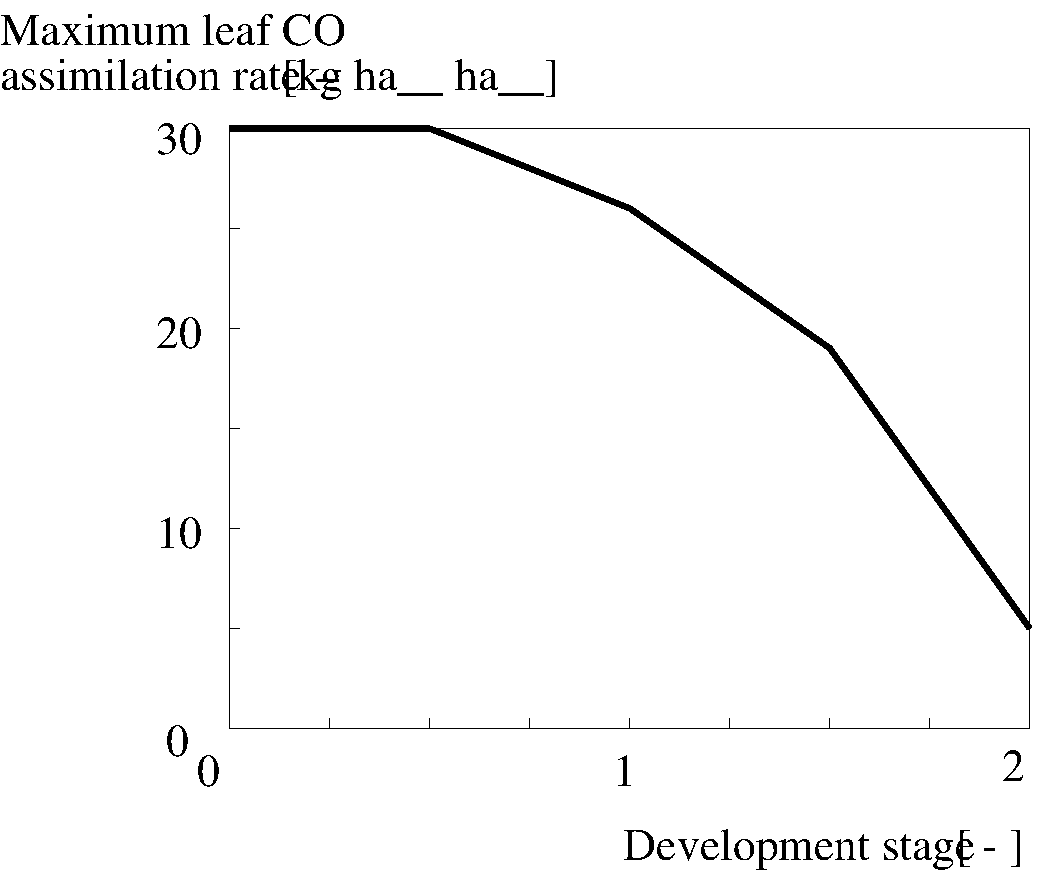
\includegraphics[width=85mm]{\FigDir/AMAXTB.pdf}
\caption{Maximum leaf CO$_{{\rm 2}}$ assimilation the rate as a function of development of
the development stage.}
\label{fig:AMAXTB}
\end{figure}

\subsubsection{Daytime temperature}
The maximum leaf CO$_{{\rm 2}}$ assimilation rate, A$_{{\rm m}}$, has to be corrected for sub-optimal average
daytime temperatures. The correction factor is determined by the average daytime
temperature and is also crop specific. An AFGEN table (acronym: {\bf TMPFTB}) with the
average day time temperature as the independent variable is used to describe this
dependency (see also Appendix 2). For an example see figure \ref{fig:TMPFTB}. 
The correction factor has to be multiplied with A$_{{\rm m}}$. The daytime temperature can be
calculated as:

\begin{equation}
% eq 5.32
T_{day} = {\frac{T_{\max} + T}{2}} ~~~~ where ~~~~ T = {\frac{T_{\max } + T_{\min}}{2}}
\end{equation}

Where:\\[5pt]
\begin{tabularx}{\textwidth}{llXr}
T$_{{\rm day}}$ &:& Average daytime temperature    &    [\degrees C]\\
T &:& (Average) daily temperature    &    [\degrees C]\\
T$_{{\rm max}}$ &:& Maximum daily temperature   &     [\degrees C]\\
T$_{{\rm min}}$  &:& Minimum daily temperature  &      [\degrees C]\\
\end{tabularx}

\begin{figure}[p]
%figure 5.4
\centering
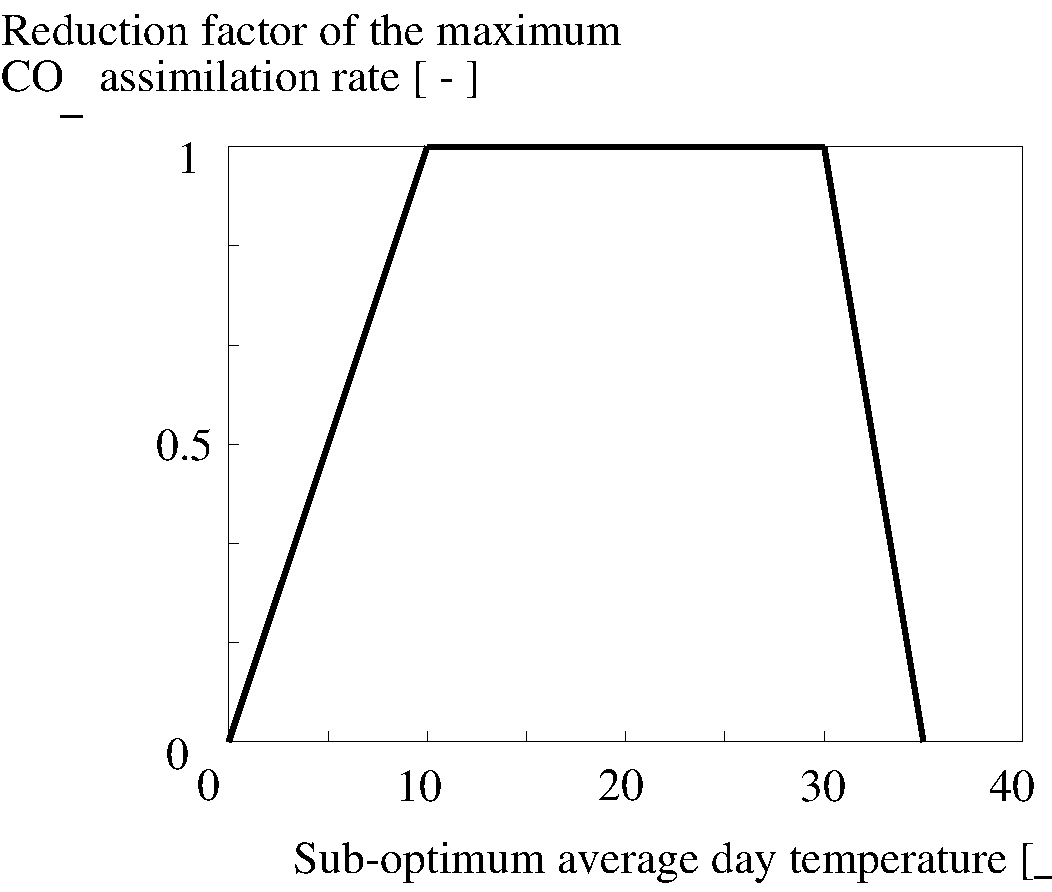
\includegraphics[width=140mm]{\FigDir/TMPFTB.pdf}
\caption{Reduction factor of the maximum leaf CO$_{{\rm 2}}$ assimilation as a function of
average temperature.}
\label{fig:TMPFTB}
\end{figure}

\subsubsection{Nighttime temperature}
The gross CO$_{{\rm 2}}$ assimilation rate cannot exceed the maximum CO$_{{\rm 2}}$ assimilation rate. It
should also be noted that assimilation is an enzymatic process and such processes are
temperature dependent (Downes, 1970). However, there seems to be a considerable
adaption of the assimilation processes to fluctuating and varying temperatures (de Wit {\it et
al.}, 1978). A wide temperature range for optimum photosynthetic performance under field
conditions is observed (Wardlaw, 1974). Low nighttime temperatures also affect the
assimilation. At night the assimilates, produced during daytime, are transformed into
structural biomass. This process is hampered by low temperature. If these low temperatures prevail 
for a several days, the assimilates accumulate in the plant and the assimilation rate diminishes 
and ultimately halts.

In the model, this temperature effect is accounted for by introducing a correction factor,
which should be multiplied with A$_{{\rm m}}$. This correction factor is a function of low minimum
temperature and is crop specific. An AFGEN table (acronym: {\bf TMNFTB}) is used to
describe this dependency.

As a measure for quantifying the effect of low minimum temperature, the seven day
running average of minimum temperature is used as the independent variable in the
AFGEN table (see also Appendix 2).

\begin{equation}
% eq 5.33
T _{low} ~=~\begin{array}{c}{i=7}  \\
\sum  \\
{i=1}\end{array}{\frac{\, T _{\min ,i} }{7}}
\end{equation}

Where:\\[5pt]
\begin{tabularx}{\textwidth}{llXr}
T$_{{\rm min}}$  &:& Daily minimum temperature   &     [\degrees C]\\
T$_{{\rm low}}$ &:& Seven day running average of minimum temperature    &    [\degrees C]\\
i &:& Day    &    [-]
\end{tabularx}


\subsubsection{Photosynthesis in terms of CH$_{{\rm 2}}$O}
In the photosynthesis process, CO$_{{\rm 2}}$ is reduced to carbohydrates (CH$_{{\rm 2}}$O) using the energy
supplied by the absorbed light. The overall chemical reaction of this complex process is:

\begin{equation}
% equation 5.34
6\, CO _{2} ~+~ 6\, H _{2} O ~\,\begin{array}{c}{light}  \\
{--->}\end{array} \, ~C _{6} H _{12} O _{6} ~+~ 6\, O _{2}
\end{equation}

or in simplified form:

\begin{equation}
% equation 5.35
CO _{2} ~+~ H _{2} O~\,\begin{array}{c}{light}  \\
{--->}\end{array} \, ~ CH _{2} O ~+~ O _{2}
\end{equation}

For each kg of CO$_{{\rm 2}}$ absorbed, 30/44 kg of CH$_{{\rm 2}}$O is formed, the numerical values
representing the molecular weights of CH$_{{\rm 2}}$O and CO$_{{\rm 2}}$ respectively.

\begin{equation}
% equation 5.36
R _{d}^{1} ~=~ A _{d}^{1} \,\,{\frac{30}{44}}
\end{equation}

Where:\\[5pt]
\begin{tabularx}{\textwidth}{llXr}
R$^{{\rm 1}}$$_{{\rm d}}$ &:& Gross daily CH$_{{\rm 2}}$O assimilation rate 
   (not corrected for water stress) &   [kg ha$^{{\rm -1}}$ d$^{{\rm -1}}$]\\
A$^{{\rm 1}}$$_{{\rm d}}$ &:& Gross daily CO$_{{\rm 2}}$ assimilation rate 
   (see eq. \ref{eq:5.11}) (corrected for low minimum temperature)   &    [kg ha$^{{\rm -1}}$ d$^{{\rm -1}}$]\\   
\end{tabularx}
 
As mentioned earlier, the gross daily CO$_{{\rm 2}}$ assimilation rate, A$^{{\rm 1}}$$_{{\rm d}}$, 
can be calculated by multiplying the total hourly instantaneous assimilation rate (eq. \ref{eq:5.31}) 
with the day length (eq. \ref{eq:AstroDaylength}). 

\subsubsection{Transpiration}
The calculated daily assimilation in CH$_{{\rm 2}}$O per ha will be reduced when water stress
occurs. In the model the effects of water stress on assimilation are related to the ratio of
actual transpiration and potential transpiration (van Keulen \& Seligman, 1987).
The gross assimilation rate, corrected for water stress, can be calculated as.

\begin{equation}
\label{eq:5.37}
R _{d} ~=~ R _{d}^{1} \,\,{\frac{T _{a} }{T _{p} }}
\end{equation}

Where:\\[5pt]
\begin{tabularx}{\textwidth}{llXr}
R$_{{\rm d}}$ &:& Gross daily CH$_{{\rm 2}}$O assimilation rate   &     
    [kg ha$^{{\rm -1}}$ d$^{{\rm -1}}$]\\
R$^{{\rm 1}}$$_{{\rm d}}$ &:& Gross daily CH$_{{\rm 2}}$O assimilation rate
   (not corrected for water stress)   &     [kg ha$^{{\rm -1}}$ d$^{{\rm -1}}$]\\
T$_{{\rm a}}$ &:& Actual transpiration   &     [cm d$^{{\rm -1}}$]\\
T$_{{\rm p}}$ &:& Potential transpiration   &     [cm d$^{{\rm -1}}$]\\
\end{tabularx}

In \S \ref{sec:evapotranspiration} the calculation of the potential, T$_{{\rm p}}$, and actual 
the transpiration, T$_{{\rm a}}$, will be explained.

\subsection{Maintenance respiration}

Some of the carbohydrates formed are respired to provide energy for maintaining the
existing biostructures. The maintenance processes include resynthesis of degraded proteins
(especially enzymes) and maintenance of ionic gradients across cell membranes. The
higher the metabolic activity of the plant, the higher the maintenance costs (Penning de
Vries, 1975), probably due to a higher enzyme turnover and higher transport costs.

Maintenance respiration provides the energy for living organisms to maintain their
biochemical and physiological status. Through the reaction which is the reverse of CO$_{{\rm 2}}$
reduction in the CO$_{{\rm 2}}$ assimilation, the radiation energy which was fixed in the
photosynthetic process is released in a suitable form (ATP and NADPH):

\begin{equation}
% eq 5.38
CH _{2} O ~+~ O _{2} ~--->~ CO _{2} ~+~ H _{2} O ~+~ energy
\end{equation}

This maintenance respiration consumes roughly 15 - 30\% of the carbohydrates produced
by a crop in a growing season (Penning de Vries {\it et al.}, 1979). This indicates the
importance of accurate quantification of this process in the model.

\subsubsection{Maintenance respiration as a function of the weight of dry matter}
The maintenance costs may be estimated on the basis of the quantities of proteins and
minerals present in the biomass and on crop metabolic activity, as presented by De Wit {\it et
al.} (1978). This method, however, requires information on the nitrogen and mineral
contents of the vegetation.
Based on the results of this analysis, typical values for the maintenance coefficients of
various plant organs have been derived by Penning de Vries \& van Laar (1982).
In the model, these coefficients are used to calculate the maintenance requirements of the
crop. According to this approach the maintenance requirements are approximately 
proportional to the dry weights of the plant organs to be maintained: 

\begin{equation}
\label{eq:5.39}
R _{m,r} ~ = ~\begin{array}{c} {i=1}  \\
\sum  \\
{i=4}\end{array} \, c _{m,i} \, W _{i}
\end{equation}

Where:\\[5pt]
\begin{tabularx}{\textwidth}{llXr}
R$_{{\rm m,r}}$ &:& Maintenance respiration rate at reference 
   temperature of 25 \degrees C &   [kg ha$^{{\rm -1}}$ d$^{{\rm -1}}$]\\
c$_{{\rm m,i}}$ &:& Maintenance coefficient of organ i  & [kg kg$^{{\rm -1}}$ d$^{{\rm -1}}$]\\
W$_{{\rm i}}$ &:& Dry matter weight organ i (see eq. \ref{eq:5.49})   &     [kg ha$^{{\rm -1}}$]\\
i &:& Leaves (lv), storage organs (so), stems (st) or roots (rt)\\ 
\end{tabularx}
 
The maintenance coefficient of organ i, {\bf c$_{{\rm m,i}}$}, is crop dependent and should be provided by
the user. Acronyms used in the model: {\bf RML} (lv), {\bf RMO} (so), {\bf RMS} (st) and {\bf RMR} (rt).

In \S \ref{sec:DMpartitioning}, $\Delta$W$_{{\rm i}}$, the increase of the dry matter weight of 
organ i per time step, will be
discussed. Integration of $\Delta$W$_{{\rm i}}$ over the previous time steps yields the total dry matter
weight of organ i (dead and alive). Integration of the net increase of dry matter, $\Delta$Wn$_{{\rm i}}$,
(see eq. \ref{eq:5.48}) over the previous time steps yields the living dry matter weight of organ i
(see eq \ref{eq:5.49}). Note that differences in nitrogen contents in the different organs cause
differences in the maintenance coefficients. However, in the model nitrogen contents are
not simulated.

\subsubsection{Dependency of the maintenance respiration on development stage}
The calculated maintenance respiration rate (eq. \ref{eq:5.39}) has to be corrected for senescence.
This correction factor is crop specific and is defined as a function of development stage
(see figure 5.5). An AFGEN table (acronym: {\bf RFSETB}) with the development stage as
independent variable, is used to describe this dependency. The maintenance respiration
should be multiplied with this factor.

\begin{figure}[htbp]
%figure 5.5
\centering
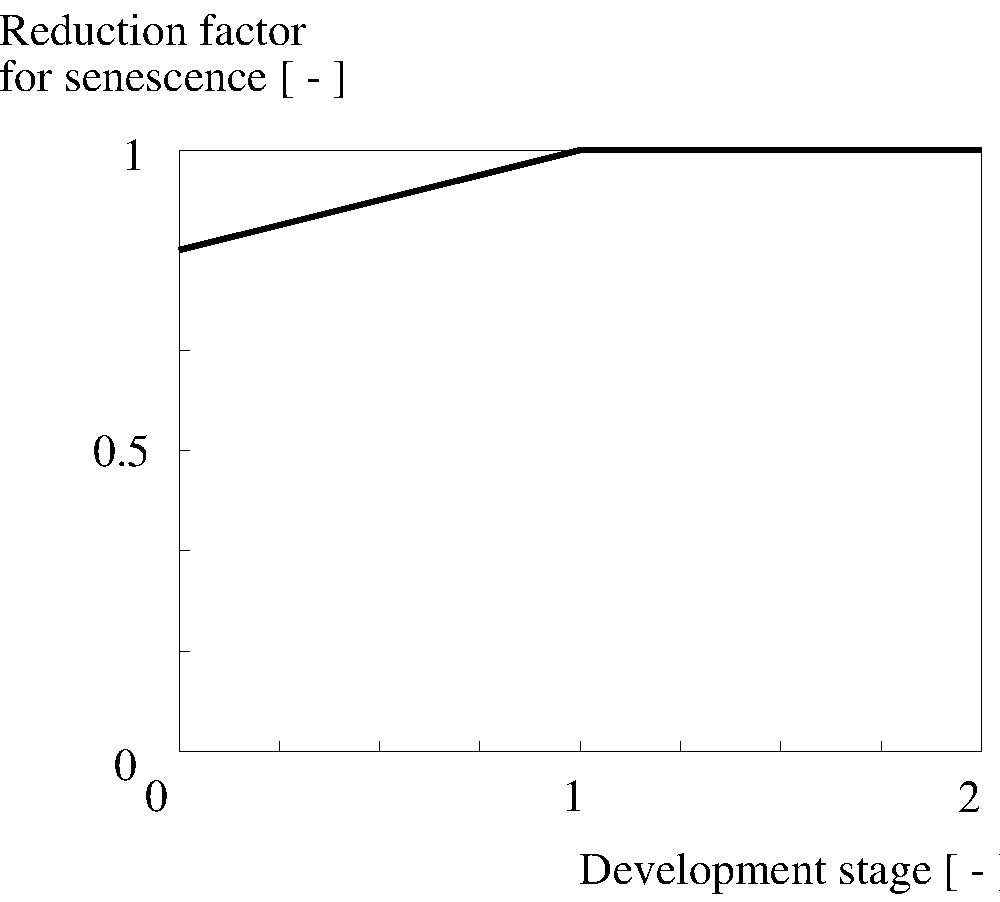
\includegraphics[width=85mm]{\FigDir/RFSETB.pdf}
\caption{Reduction factor for senescence as a function of development stage}
\label{fig:RFSETB}
\end{figure}

\subsubsection{Dependency of the maintenance respiration on temperature}
Higher temperatures accelerate the turnover rates in plant tissue and hence the costs of
maintenance. An increase in temperature of 10\degrees C increases maintenance respiration by a
factor of about 2 (Kase \& Catsky, 1984; Penning de Vries \& van Laar, 1982). However,
in order to be more flexible, in the model a variable {\bf Q$_{{\rm 10}}$} (acronym: {\bf Q10}) is introduced.
Q$_{{\rm 10}}$ is defined as the relative increase of the respiration rate per 10\degrees C temperature
increase. Q$_{{\rm 10}}$ should be provided by the user. The rate of the maintenance respiration at a
certain temperature, can be calculated with:

\begin{equation}
\label{eq:5.40}
R _{m,T} ~=~ R _{m,r} \, Q _{10}^{~~{\frac{T-T _{r} }{10}} }
\end{equation}
 
Where:\\[5pt]
\begin{tabularx}{\textwidth}{llXr}
R$_{{\rm m,T}}$ &:& Maintenance respiration rate at 
    temperature T &    [kg ha$^{{\rm -1}}$ d$^{{\rm -1}}$]\\
R$_{{\rm m,r}}$ &:& Maintenance respiration rate at reference 
    temperature of 25 \degrees C (see eq. \ref{eq:5.39})   &     [kg ha$^{{\rm -1}}$ d$^{{\rm -1}}$]\\
Q$_{{\rm 10}}$ &:& Relative increase of the respiration rate
    per 10\degrees C temperature increase    &    [-]\\
T &:& Average daily temperature    &     [\degrees C]\\
T$_{{\rm r}}$ &:& Reference temperature {\small [=25 \degrees C in 
    the model]}    &    [\degrees C]\\
\end{tabularx}

 
For tropical species, the reference temperature may be 10\degrees C higher than for species from
temperate climates. The maintenance requirements of a crop are likely to be adapted to
the higher growth temperatures. However, in WOFOST 6.0 the reference temperature is
fixed at 25\degrees C for all crops.

As stated before, maintenance respiration rate depends on the amount of dry matter in the
various organs, the relative maintenance rate per organ and the temperature. It cannot
exceed the actual gross assimilation rate. It is assumed that the vegetation will not be
'self-consuming' in terms of carbohydrates. Actual gross assimilation rate minus 
maintenance respiration rate results in the amount of assimilates available for conversion into
structural material. When the crop ages, its metabolic activity and therefore its
maintenance requirements decreases. This effect could be accounted for by relating 
the maintenance coefficients to the N content of the tissues (van Keulen \& Seligman, 1987).
However, N contents are not simulated in the model. 

\subsection{Growth respiration}

The primary assimilates in excess of the maintenance costs, are for conversion into
structural plant material. In this conversion process of the glucose molecules, CO$_{{\rm 2}}$ and
H$_{{\rm 2}}$O are released. This is a partial combustion of glucose to provide energy required in
the various biochemical pathways. Hence, biosynthesis of the various structural compounds can 
be considered a process of cut and paste, the scraps representing the weight
lost in growth respiration.
Each structural compound is formed along a distinct, non crop-specific pathway.
Following these reactions, the weight of glucose required to produce a unit of the
compound can be calculated (Penning de Vries {\it et al.}, 1974). The transport costs of the
molecules are included. Two active passages of membranes are assumed. Each active
passage requires 1 ATP, which is provided by respiring $^{{\rm 1}}$/$_{{\rm 3}}$$_{{\rm 8}}$ molecule of glucose.

The assimilates required to produce a unit weight of a certain plant organ can now be
calculated from its chemical composition and the assimilate requirements of the various
chemical compounds. Storage organs (grains, tubers, etc.) vary to much in composition
among species for one general value of their assimilate requirements to be given. The
conversion efficiency represents the inverse of the assimilate requirement.

At higher temperatures the conversion processes are accelerated, but the pathways are
identical (Spitters {\it et al.} 1989). Hence, the assimilate requirements do not vary with
temperature. The growth respiration rate can then be calculated as:

\begin{equation}
\label{eq:5.41}
R _{g} ~=~ R _{d} ~-~ R _{m,T} 
\end{equation}

Where:\\[5pt]
\begin{tabularx}{\textwidth}{llXr}
R$_{{\rm g}}$ &:& Growth respiration rate   &     [kg ha$^{{\rm -1}}$ d$^{{\rm -1}}$]\\
R$_{{\rm d}}$ &:& Actual daily CH$_{{\rm 2}}$O assimilation rate (see eq. \ref{eq:5.37})   &   
    [kg ha$^{{\rm -1}}$ d$^{{\rm -1}}$]\\
R$_{{\rm m,T}}$ &:& Maintenance respiration rate at 
    temperature T (see eq. \ref{eq:5.40})   &     [kg ha$^{{\rm -1}}$ d$^{{\rm -1}}$]\\
\end{tabularx}

\subsection{Dry matter partitioning  }
\label{sec:DMpartitioning}

As explained, conversion into dry matter costs energy, therefore a conversion factor is
defined. This factor depends on the conversion efficiency of assimilates and on the
partitioning factors of the different organs. The dry matter is multiplied with this overall
conversion efficiency factor to calculate the dry matter increase. The conversion 
efficiency of carbohydrates into structural plant material is calculated as a weighted average
of the efficiencies for the various plant organs.

\begin{equation}
\label{eq:5.42}
C _{e} ~={\frac{~1}{
        \begin{array}{c}
        {i=3}  \\
        \sum  \\
        {i=1}
        \end{array} {pc_{i}}/{C_{e,i}} \cdot (1-pc_{rt} ) + {pc_{rt}}/{C_{e,rt}} 
        }}
\end{equation}

Where:\\[5pt]
\begin{tabularx}{\textwidth}{llXr}
C$_{{\rm e}}$ &:& Conversion efficiency factor of assimilates, total crop  &   
    [kg kg$^{{\rm -1}}$]\\
C$_{{\rm e,i}}$ &:& Conversion efficiency factor of the assimilates 
    of a specified organ  &      [kg kg$^{{\rm -1}}$]\\
pc$_{{\rm i}}$ &:& Partitioning factor of organ i   &
     [kg kg$^{{\rm -1}}$]\\
i &:& Leaves (lv), storage organs (so), stems (st)\\
rt &:& roots\\
\end{tabularx}

The conversion efficiency factor for the assimilates of a specified organ, {\bf C$_{{\rm e,i}}$}, is crop
specific and should be given by the user. Acronyms used in the model: {\bf CVL} (lv), {\bf CVO}
(so), {\bf CVR} (rt) and {\bf CVS} (st).

The dry matter growth rate of the total crop can be calculated as:

\begin{equation}
% eq 5.43
\Delta W~=~ C_{e} \cdot R_{g} 
\end{equation}

Where:\\[5pt]
\begin{tabularx}{\textwidth}{llXr}
$\Delta$W &:& Dry matter growth rate total crop   &
    [kg ha$^{{\rm -1}}$ d$^{{\rm -1}}$]\\
C$_{{\rm e}}$ &:& Conversion efficiency factor of assimilates,
    total crop (see eq. \ref{eq:5.42})    &    [kg kg$^{{\rm -1}}$] \\
R$_{{\rm g}}$ &:& Growth respiration rate (see \ref{eq:5.41})   &
     [kg ha$^{{\rm -1}}$ d$^{{\rm -1}}$]\\
\end{tabularx}

The pattern of dry matter distribution over the various plant organs is closely related to
the development stage of the crop. Development is defined as progression in the successive 
phenological stages. It is characterized by the formation rate of the various vegetative
and reproductive organs and their order of appearance.

The amount of the absorbed CH$_{{\rm 2}}$O that remains after correction and reduction of the
gross CO$_{{\rm 2}}$ assimilation rate is the so called dry matter. Growth, in fact is the increase in
biomass ignoring its water content. The dry matter is partitioned over the 4 parts of the
plant. In the model, total dry matter growth is partitioned according to fixed distribution
factors, defined as a function of development stage. Dry matter is first partitioned
between shoots and roots. 

\stepcounter{equation}
\begin{align}
% eqn 5.44a,b
\Delta W_{rt} &= pc_{rt} \cdot \Delta W   \subeqn  \\
\Delta W_{sh} &= (1 - pc_{rt}) \Delta W \subeqn
\end{align}

 
Where:\\[5pt]
\begin{tabularx}{\textwidth}{llXr}
$\Delta$W &:& Dry matter growth rate total crop   &
     [kg ha$^{{\rm -1}}$ d$^{{\rm -1}}$]\\
$\Delta$W$_{{\rm rt}}$ &:& Dry matter growth rate roots    &
    [kg ha$^{{\rm -1}}$ d$^{{\rm -1}}$]\\
$\Delta$W$_{{\rm sh}}$ &:& Dry matter growth rate shoots    &
    [kg ha$^{{\rm -1}}$ d$^{{\rm -1}}$]\\
pc$_{{\rm rt}}$ &:& Partitioning factor of roots    &
    [kg kg$^{{\rm -1}}$]\\
\end{tabularx}

The growth rate of leaves, stems and storage organs is simply the product of the dry
matter growth rate of the shoots and the fraction allocated to these organs.

\begin{equation}
\label{eq:5.45}
\Delta W_{i} ~=~ pc_{i} \cdot \Delta W_{sh} 
\end{equation}

Where:\\[5pt]
\begin{tabularx}{\textwidth}{llXr}
$\Delta$W$_{{\rm i}}$ &:& Dry matter growth rate of organ i &
    [kg ha$^{{\rm -1}}$ d$^{{\rm -1}}$]\\
$\Delta$W$_{{\rm sh}}$ &:& Dry matter growth rate of shoots   &
    [kg ha$^{{\rm -1}}$ d$^{{\rm -1}}$]\\
pc$_{{\rm i}}$ &:& Partitioning factor of organ i    &
    [kg kg$^{{\rm -1}}$]\\
i &:& Leaves (lv), storage organs (so), stems (st)
\end{tabularx}

The partitioning factors, {\bf pc$_{{\rm i}}$}, are a function of development stage and are crop specific. In
the model, the dependency is described using AFGEN tables with the development stage
as the independent variable (see Appendix 2). Acronyms used in the model: {\bf FLTB} (lv),
{\bf FOTB} (so), {\bf FRTB} (rt) and {\bf FSTB} (st).

At any development stage the following relation must be valid, if not, the simulation will
be stopped (see also fig. 5.6):

\begin{equation}
% eq 5.46
pc_{lv} + pc_{st} + pc_{so} = 1
\end{equation}

Where:\\[5pt]
\begin{tabularx}{\textwidth}{llXr}
pc$_{{\rm i}}$ &:& Partitioning factor of organ i   &
     [kg kg$^{{\rm -1}}$]\\
i &:& Leaves (lv), storage organs(so), stems (st)
\end{tabularx}

\begin{figure}[p]
% fig 5.6
\centering
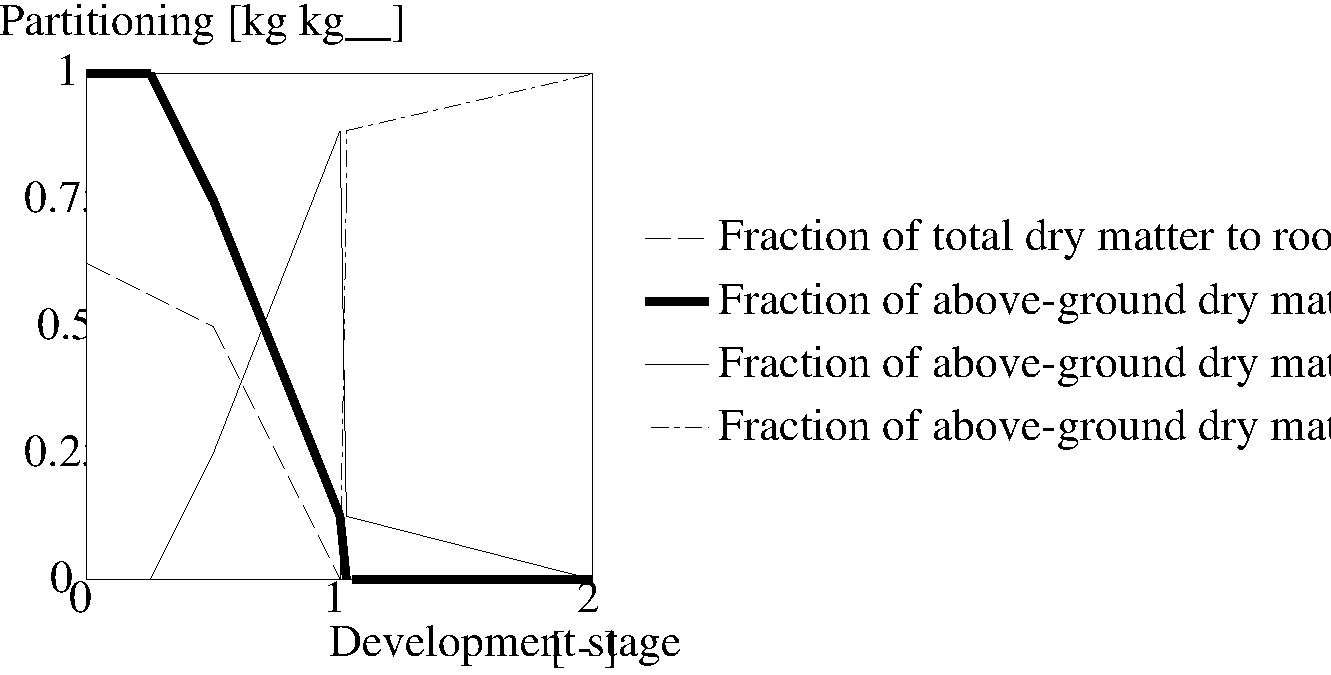
\includegraphics[width=120mm]{\FigDir/FRTB.pdf}
\caption{Partitioning factors of the different organs as a function of development stage}
\label{fig:partitioning}
\end{figure}

The actual gross CO$_{{\rm 2}}$ assimilation rate has to be identical to the amount of structural plant
material produced plus the amounts used for maintenance respiration and conversion (see
figure 5.1). The carbon balance has to be zero. 

\begin{equation}
\label{eq:5.47}
0 = {\frac{R_{d} - R_{m,T} - R_{g} \big( pc_{rt} + (pc_{lv} + pc_{st} + pc_{so}) \cdot (1 - pc_{rt}) \big) }{R_d}}  
\end{equation}

Where:\\[5pt]
\begin{tabularx}{\textwidth}{llXr}
R$_{{\rm g}}$ &:& Growth respiration rate (see eq. \ref{eq:5.41})   &
     [kg ha$^{{\rm -1}}$ d$^{{\rm -1}}$]\\
R$_{{\rm d}}$ &:& Actual daily CH$_{{\rm 2}}$O assimilation rate (see eq. \ref{eq:5.37})   &
     [kg ha$^{{\rm -1}}$ d$^{{\rm -1}}$]\\
R$_{{\rm m,T}}$ &:& Maintenance respiration rate (see eq. \ref{eq:5.40})   &
     [kg ha$^{{\rm -1}}$ d$^{{\rm -1}}$]\\
pc$_{{\rm i}}$ &:& Partitioning factor of organ i    &
     [kg kg$^{{\rm -1}}$]\\
i &:& Leaves (lv), storage organs (so), stems (st), roots (rt)\\
\end{tabularx}

As mentioned earlier, it is assumed that maintenance respiration can not exceed the actual
gross assimilation rate. However, in case the daily CH$_{{\rm 2}}$O assimilation rate comes close to
zero, this might happen and therefore simulation should be stopped. Introducing a
division by R$_{{\rm d}}$ in the carbon check (eq. \ref{eq:5.47}) will identify the occurrence of such an
event.It should be mentioned that in subsequent versions of the WOFOST model, the carbon
balance check will be simplified.

\subsection{Growth and leaf senescence  }
\label{sec:5.4.5}

As is explained in paragraph \ref{sec:DMpartitioning}, the growth rate of a certain plant organ is obtained by
multiplying the growth rate of either shoot or root by the fraction allocated to that organ.
Its total dry biomass (dead and alive) is obtained by integrating this growth rate over
time. Taking the death rate of the different organs into account, the integration of the net
increase of dry matter, $\Delta$Wn$_{{\rm i}}$, (see eq. \ref{eq:5.48}) over the previous time steps 
yields the living dry matter weight of organ i (see eq. \ref{eq:5.49}).

This approach of the partitioning of dry matter is descriptive, as the distribution keys are
defined as a function of the development stage of the crop only. The influence of
environmental factors could be included by applying modification factors to these keys,
depending on temperature, water and nutrient status of the crop, and its reserve level
(Loomis {\it et al.}, 1979; van Keulen \& Seligman, 1987). In the WOFOST model, however,
this is not applied. Some more attention is paid to the crop growth by introducing a death
rate for leaves, roots and stems. Death rate is a function of the development stage of the
plant and is crop and organ specific.

\subsubsection{Growth and growth rate}
In the model, the death rate of the storage organs is considered to be zero. For the roots
and the stems increase in living biomass can be easily determined as the growth rate
minus death rate. This yields the net growth rate (eq. \ref{eq:5.48}). The death rate is crop
specific and is defined as the daily amount of the living biomass which no longer
participates in the plant processes. The death rate of stems and roots is considered to be a
function of development stage (see fig. \ref{fig:DeathRoots}). This dependency is described using an
AFGEN table with the development stage as the independent variable (see also Appendix
2). The death rate of leaves is more complicated. Leaf senescence due to shading (high
LAI), water stress and also due to exceedance of the life span should be accounted for.


\begin{figure}[p]
%Fig. 5.7
\centering
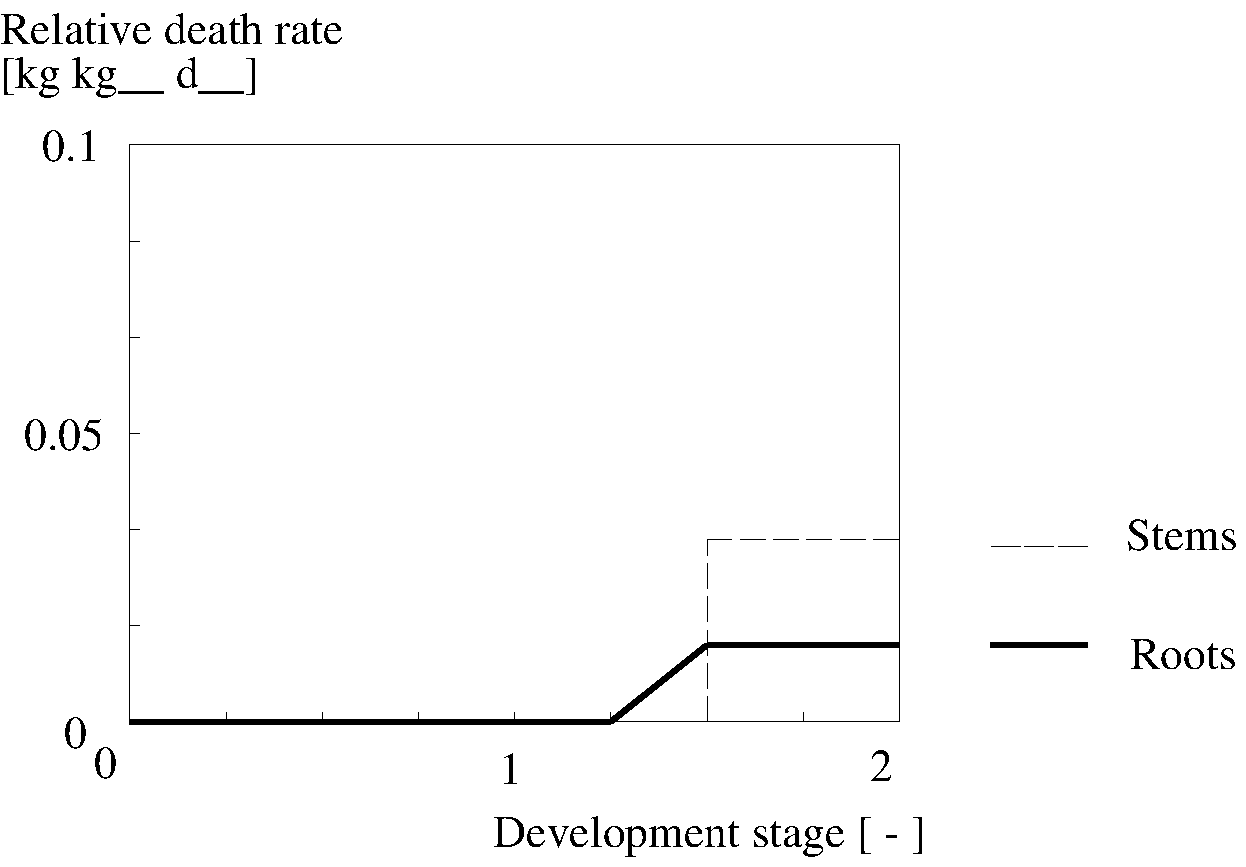
\includegraphics[width=100mm]{\FigDir/RDRRTB.pdf}
\caption{Death rate of roots and stems as a function of development rate}
\label{fig:DeathRoots}
%\begin{forcewidth}{10.05cm}
% \begin{center}\InputPS{\FigDir/RDRRTB.eps} \end{center}
%\end{forcewidth}
\end{figure}


The net growth rate of the stems and roots can described by:

\begin{equation}
\label{eq:5.48}
\Delta Wn _{i~} =~\,\,\Delta W _{i~} -~ {\rm \dag } _{i} \,\, W _{i} 
\end{equation}

Where:\\[5pt]
\begin{tabularx}{\textwidth}{llXr}
$\Delta$Wn$_{{\rm i}}$ &:& Net dry matter growth rate of organ i   &
    [kg ha$^{{\rm -1}}$ d$^{{\rm -1}}$]\\
$\Delta$W$_{{\rm i}}$ &:& Dry matter growth rate of organ i (see eq. \ref{eq:5.45})   &
    [kg ha$^{{\rm -1}}$ d$^{{\rm -1}}$]\\
W$_{{\rm i}}$ &:& Dry matter weight organ i  &
    [kg ha$^{{\rm -1}}$]\\
\dag $_{{\rm i}}$ &:& Death rate organ i   &
    [kg kg$^{{\rm -1}}$ d$^{{\rm -1}}$]\\
i &:& Stems (st), roots (rt)\\
\end{tabularx}

The death rates of stems and roots are crop specific and should be provided by the user.
A dependency of the development stage is assumed. AFGEN tables (acronym: {\bf RDRRTB}
(rt), {\bf RDRSTB} (st)) with the development stage as the independent variable are used to
describe this dependency.

Although the process which describes the death rate of leaves is more complicated than
the calculation of the death rate of stems and roots, the calculation to establish the total
dry weight of living leaves is the same as the computation of the dry matter weight of
stems and roots. The total dry matter weight of living leaves, stems and roots can be
found by integration over time of the net dry matter growth, $\Delta$Wn$_{{\rm i}}$, yields 
the dry matter.

\begin{equation}
\label{eq:5.49}
W _{t,i} ~=~W _{t-1\, ,\, i} ~+~\Delta Wn _{i} \,\Delta t
\end{equation}

Where:\\[5pt]
\begin{tabularx}{\textwidth}{llXr}
W$_{{\rm i,t}}$ &:& Dry matter weight organ i at time step t   &
     [kg ha$^{{\rm -1}}$]\\
$\Delta$Wn$_{{\rm i}}$ &:& Net dry matter growth rate of organ i   &
     [kg ha$^{{\rm -1}}$ d$^{{\rm -1}}$]\\
$\Delta$t &:& Times step   &
     [d]\\
i &:& Stems (st), roots (rt), leaves (lv)\\
\end{tabularx}

The equation \ref{eq:5.49} is recursive. In the model, the initial values of the dry weight of the
various organs are calculated. An initial value for the total dry weight of the crop
(acronym: {\bf TDWI}) should be provided by the user. This value is multiplied by the
partioning factors, pc$_{{\rm i}}$, at emergence, yielding the initial values of dry weight of the
various organs.

\subsubsection{Growth of leaves}
The area of green leaves is the major determinant for light absorption and photosynthesis
of the crop. Under optimal conditions, light intensity and temperature are the environmental factors influencing the rate of leaf area expansion. Light intensity determines the
rate of photosynthesis and hence the supply of assimilates to the leaves.

Temperature affects the rates of cell division and extension (Ng \& Loomis, 1984; Sheehy
{\it et al.}, 1980; Acock {\it et al.}, 1978). During the early stages of crop growth, temperature is
the overriding factor. The rate of leaf appearance and final leaf size are constrained by
temperature through its effect on cell division and extension, rather than by the supply of
assimilates (Hunt, 1982; Causton \& Venus, 1981; van Dobben, 1962). The growth curve
in the early stage has an exponential form. Some unpublished field data have shown that
the exponential model should be restricted to the situation where the development stage, 
D$_{{\rm s,t}}$ $<$ 0.3 and LAI $<$ 0.75 (see also eq. \ref{eq:5.4}). In the model, however, it is assumed that
the exponential growth rate of the leaf area index is valid until the source-limited increase
of the leaf area index equals the exponential growth rate.

The growth rate of the leaf area index per time step in the early, exponential growth
stage, can be calculated as:

\begin{equation}
% eq:5.50
L _{Exp,t} ~=~LAI _{{t~RL~T}_{e}}
\end{equation}

Where:\\[5pt]
\begin{tabularx}{\textwidth}{llXr}
L$_{{\rm Exp,t}}$ &:& Growth rate of the leaf area index at time step t
    during exponential growth stage   &    [ha ha$^{{\rm -1}}$ d$^{{\rm -1}}$]\\
LAI$_{{\rm t}}$ &:& Leaf area index at time step t    &
    [ha ha$^{{\rm -1}}$]\\
RL &:& Maximum relative increase of leaf area index   &
    [\degrees C$^{{\rm -1}}$ d$^{{\rm -1}}$]\\
T$_{{\rm e}}$ &:& Daily effective temperature (see 5.2c)   &
    [\degrees C]\\
\end{tabularx}

In theory, the maximum relative increase of the leaf area index, {\bf RL}, is a function of
effective temperature. For a relative wide range of temperatures {\bf RL} responds more or
less linearly to temperature (Hunt {\it et al.}, 1985; Causton \& Venus, 1981; van Dobben,
1962). In the model however, a fixed value per crop type is assumed (acronym: 
{\bf RGRLAI}). This value should be given by the user.

The accumulated leaf area index at time step t during the exponential growth stage can be
described as:

\begin{equation}
\label{eq:5.51}
LAI _{t~} =~LAI _{t-1} ~+~L _{Exp\, ,\, t} ~\Delta t
\end{equation}

Where:\\[5pt]
\begin{tabularx}{\textwidth}{llXr}
L$_{{\rm Exp,t}}$ &:& Growth rate of the leaf area index at time step t
    during exponential growth stage    &    [ha ha$^{{\rm -1}}$ d$^{{\rm -1}}$]\\
LAI$_{{\rm t}}$ &:& Leaf area index at time step t   &
    [ha ha$^{{\rm -1}}$]\\
$\Delta$t &:& Time step   &    [d]
\end{tabularx}

The equation\ref{eq:5.51} is recursive. In the model, {\bf LAI$_{{\rm t}}$} is initialized by 
setting the starting
value equal to the leaf area index at emergence (acronym: {\bf LAIEM}). The leaf area index
at emergence is crop specific and should be provided by the user.

During the development of the crop, leaf area expansion is increasingly restricted by
assimilate supply (i.e. source limited increase). Branching and tillering generate an
increasing number of sites per plant, where leaf initiation can take place. As mentioned
earlier, in the model it is assumed that the exponential growth rate of leaf area index will
continue until it equals the source limited growth rate of the leaf area index.

The growth rate of the leaf area index at time step t during the source limited growth 
stage can be described by:

\begin{equation}
\label{eq:5.52}
L _{Sc,t} ~=~\Delta Wn _{lv} ~S _{la} 
\end{equation}

Where:\\[5pt]
\begin{tabularx}{\textwidth}{llXr}
L$_{{\rm Sc,t}}$ &:& Growth rate of the leaf area index at time step t
    during the source limited growth stage    &
    [ha ha$^{{\rm -1}}$ d$^{{\rm -1}}$]\\
$\Delta$Wn$_{{\rm lv}}$ &:& Net dry matter growth of leaves at time step t    &
    [kg ha$^{{\rm -1}}$ d$^{{\rm -1}}$]\\
S$_{{\rm la}}$ &:& Specific leaf area at time step t   &
    [ha kg$^{{\rm -1}}$]\\
\end{tabularx}
 
The net dry matter growth of leaves, $\Delta$Wn$_{{\rm lv}}$, can be found by subtracting the weight of
leaves which died during the current time step from the dry matter growth of leaves,
$\Delta$W$_{{\rm lv}}$. This process will be described later in more detail in this paragraph.

The specific leaf area, {\bf S$_{{\rm la}}$} (acronym: {\bf SLATB}), is defined as the increase of the leaf area
of the crop per kg weight increase of the living leaves. S$_{{\rm la}}$ is crop specific and a function
of the development stage (see figure 8). In the model this dependency is described using
an AFGEN table with the development stage as the independent variable (see also
Appendix 2).

The accumulated leaf area index at time step t during the source limited growth stage can
be described as:

\begin{equation}
\label{eq:5.53}
LAI _{t~} =~LAI _{t-1} ~+~L _{Sc\, ,\, t} ~\Delta t
\end{equation}

Where:\\[5pt]
\begin{tabularx}{\textwidth}{llXr}
L$_{{\rm Sc,t}}$ &:& Growth rate of the leaf area index at time step t
    during the source limited growth stage     &   [ha ha$^{{\rm -1}}$ d$^{{\rm -1}}$]\\
LAI$_{{\rm t}}$ &:& Leaf area index at time step t     &
    [ha ha$^{{\rm -1}}$]\\
$\Delta$t &:& Time step    &    [d]\\
\end{tabularx}
 
The equation \ref{eq:5.53} is recursive. In the model, {\bf LAI$_{{\rm t}}$} is initialized by 
setting the starting
value equal to the leaf area index at emergence (acronym: {\bf LAIEM}). The leaf area index
at emergence is crop specific and should be provided by the user.

In the model, however, the accumulated leaf area cannot be calculated directly. The leaf
area index has to be corrected for leaf senescence which occurred during the current time
step. The leaf senescence can be caused by physiological ageing, water stress and/or high
leaf area index (i.e. mutual shading). Later in this text, more attention will be paid to
these effects.

In order to correct for leaf senescence, the specific leaf area of each time step, S$_{{\rm la}}$, the
growth of the dry matter weight of leaves per time step, $\Delta$W$_{{\rm lv}}$ and the physiological age,
P$_{{\rm age}}$ (see eq. \ref{eq:5.57}), have to be stored in three different arrays. These arrays are organized
as follows: the first element of the arrays represents the most recent age class (or time
step) and the last element of the arrays represents the oldest age class (or time step). It
should be clear that the position of an element in the arrays represents its age class, in
time steps. The dry matter weight of the leaves, which have died during the current time
step, has to be. subtracted from the growth of dry matter weight per time step. One array
contains thus the net dry matter growth of the leaves per time step, $\Delta$Wn$_{{\rm lv}}$. 
The procedure which describes this process will be explained later in this text. 

After the correction for leaf senescence, the accumulated leaf area can be established. The
net dry matter weight of the leaves, $\Delta$Wn$_{{\rm lv,}}$  in the remaining and new leaf classes is
multiplied with the specific leaf areas (see eq. \ref{eq:5.52}) to get the growth rate of the leaf area
index of the living leaves per age class. Multiplication with $\Delta$t and summation over the
classes (eq. \ref{eq:5.53}) yields the total leaf area index. The green area index of the stems and
the storage organs is added to this amount. The total dry matter weight of living leaves
can be found in a similar way by using equation \ref{eq:5.49}.

\begin{figure}[p]
%Fig. 5.8   
\centering
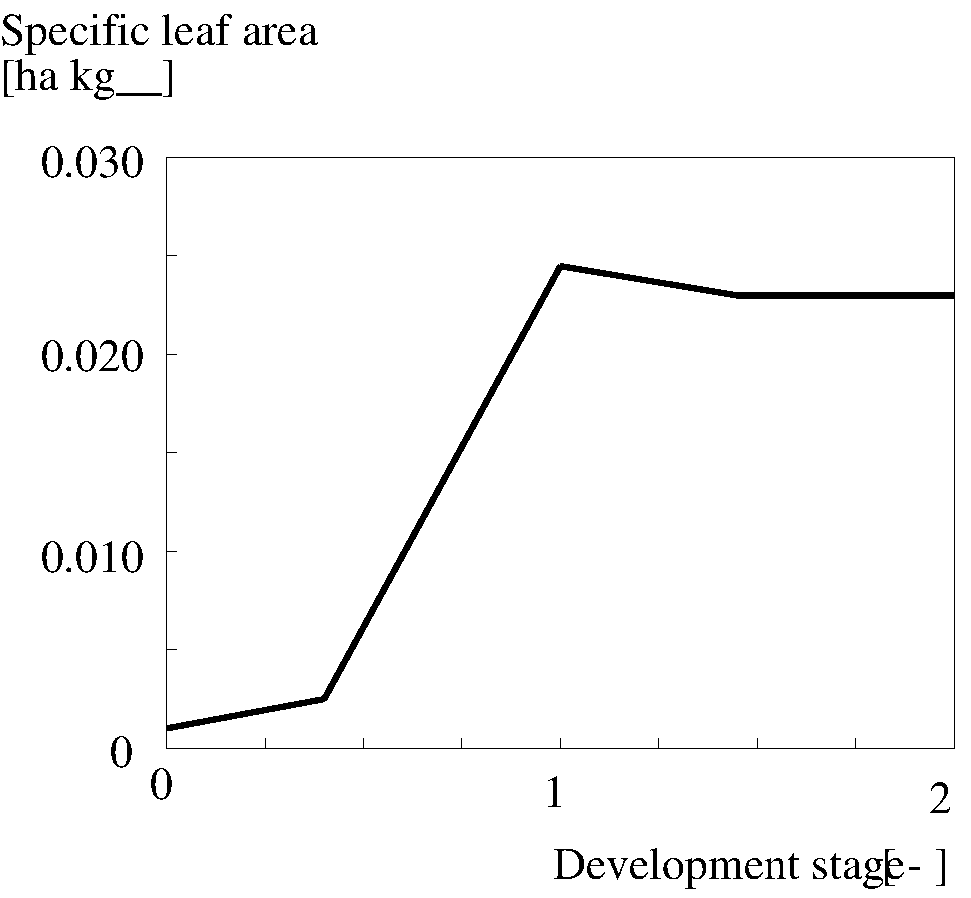
\includegraphics[width=120mm]{\FigDir/SLATB.pdf}
\caption{Specific leaf area as a function of development stage}
\label{fig:SpecificLeafArea}
%\begin{forcewidth}{10.05cm}
% \begin{center}\InputPS{\FigDir/SLATB.eps} \end{center}
%\end{forcewidth}
\end{figure}

As is mentioned earlier, the green area index of the stems and storage organs, may absorb
a substantial amount of radiation. Therefore it should be added to the total leaf area
index. The green area index of these organs can be calculated by:

\begin{equation}
% eq:5.54
GAI_{i} ~=~SS _{i} W _{i} 
\end{equation}

Where:\\[5pt]
\begin{tabularx}{\textwidth}{llXr}
GAI$_{{\rm i}}$ &:& Green area index of organ i    &
    [ha ha$^{{\rm -1}}$]\\
SS$_{{\rm i}}$ &:& Specific green area of organ i    &
    [ha kg$^{{\rm -1}}$]\\
W$_{{\rm i}}$ &:& Dry matter organ i (see eq. \ref{eq:5.49})    &
    [kg ha$_{{\rm -1}}$]\\
i &:& Stems (st), storage organs (so)\\
\end{tabularx}

The specific green area of stems (acronym: {\bf SSA}) and storage organs (acronym: {\bf SPA}) are
crop specific and should be provided by the user. The specific storage organ area is also
known as the specific pod area.

Special attention should be paid to the fact that during the exponential growth stage, the
specific leaf is not established. Therefore, during this period, for each time step, the
specific leaf area has to be calculated according to:

\begin{equation}
% eq:5.55
S_{\exp,t} ~=~ {\frac{L_{\exp,t}}{\Delta W_{lv} }}
\end{equation}

Where:\\[5pt]
\begin{tabularx}{\textwidth}{llXr}
S$_{{\rm exp,t}}$ &:& Specific leaf area at time step t during the 
    exponential growth stage    &     [ha kg$^{{\rm -1}}$]\\
$\Delta$W$_{{\rm lv}}$ &:& Dry matter increase of leaves (see eq. \ref{eq:5.45})   &
    [kg ha$_{{\rm -1}}$ d$^{{\rm -1}}$]\\
L$_{{\rm \exp,t}}$ &:& Growth rate of the leaf area index at time step t
   during exponential growth stage (see eq. \ref{eq:5.51})   &
        [ha ha$^{{\rm -1}}$ d$^{{\rm -1}}$]\\
\end{tabularx}

 
In de model, it is assumed that senescence does not occur during the exponential growing
stage. This means that $\Delta$W$_{{\rm lv}}$ can be used in stead of the net dry matter growth, $\Delta$Wn$_{{\rm lv}}$.

\subsubsection{Leaf senescence}
As stated before, leaf senescence is more complicated. Senescence refers to the loss of
capacity to carry out essential physiological processes and to the loss of living biomass.
The fundamental processes involve physiological ageing and protein breakdown. These
processes are difficult to quantify. Leaves are assumed to die when they have completed
their life cycle. The dying rate may be accelerated as a result of drought stress or of
mutual shading.

{\it physiologic ageing}\\
Leaves die due to exceedance of the life span for leaves (i.e. physiologic ageing). Life
span is defined as the maximum time in days a leaf can live at a constant temperature of
35\degrees C. Life span is crop specific. The concept of lifespan is compatible with a definition
in terms of temperature sum as given by Gallagher (1979).
The physiologic ageing factor per time step can be calculated as:

\begin{equation}
% eq:5.56
f _{rai} ~=~{\frac{ T~-~T _{b\, ,\, age} }{35~-~ T _{b\, ,\, age} }}
\end{equation}

Where:\\[5pt]
\begin{tabularx}{\textwidth}{llXr}
f$_{{\rm rai}}$ &:& Physiologic ageing factor for leaf age increase   &
    [-]\\
T &:& Daily (average) temperature   &
    [\degrees C]\\
T$_{{\rm b,age}}$ &:& Lower threshold temperature for physiologic ageing   &
    [\degrees C]\\
\end{tabularx}

The lower threshold temperature for physiologic ageing, {\bf T$_{{\rm b,age}}$} (acronym: {\bf TBASE}), is
crop specific and should be provided by the user. The integral of the physiologic ageing
factor over time yields the physiologic age. 

\begin{equation}
\label{eq:5.57}
P _{age,t} ~=~ P _{age,t-1} ~+~f_{rai} \Delta t
\end{equation}

Where:\\[5pt]
\begin{tabularx}{\textwidth}{llXr}
P$_{{\rm age,t}}$ &:& Physiologic age at time step t & [d]\\
f$_{{\rm rai}}$ &:& Physiologic ageing factor for leaf age increase & [-]\\
$\Delta$t &:& time step & [d]\\
\end{tabularx}

Leaves may attain the age defined by the crop specific life span (acronym: {\bf SPAN}).
However, as is mentioned earlier, they can not exceed it. In the model the ages of the
leaf classes are checked. The first class younger than the defined life span becomes the
oldest class. Note that death of old leaves takes place after ageing, being the result of the
daily shifting from one leaf class to the next (Johnson \& Thornley, 1983). In this way,
the life time of leaves is the maximum number of days that a leaf class contributes to the
LAI and to photosynthesis.

{\it Death rate due to water stress}\\
The potential death rate of leaves due to water stress can be calculated as:

\begin{equation}
% eq:5.58
\Delta W_{d}^{1} ~=~ W_{lv} \, (\, 1\, -\,{\frac{T _{a} }{T _{p} }} \, )\, {\rm \dag } _{\max ,lv} 
\end{equation}

Where:\\[5pt]
\begin{tabularx}{\textwidth}{llXr}
$\Delta$W$^{{\rm 1}}$$_{{\rm d}}$ &:& Potential death rate of leaves due to water stress   &
    [kg  ha$^{{\rm -1}}$ d$^{{\rm -1}}$]\\
\dag $_{{\rm max,lv}}$ &:& Maximum relative death rate of leaves due to
    water stress   &     [kg kg$^{{\rm -1}}$ d$^{{\rm -1}}$]\\
W$_{{\rm lv}}$ &:& Dry matter weight of the leaves (see eq. \ref{eq:5.49})  &
    [kg ha$^{{\rm -1}}$]\\
T$_{{\rm a}}$ &:& Actual transpiration (see \S \ref{sec:evapotranspiration})    &
    [cm d$^{{\rm -1}}$]\\
T$_{{\rm p}}$ &:& Potential transpiration (see \S \ref{sec:evapotranspiration})   &
    [cm d$^{{\rm -1}}$]\\
\end{tabularx}
 
The maximum relative death rate of leaves due to water stress, {\bf \dag $_{{\rm max,lv}}$} 
(acronym: {\bf PERDL}) is crop specific and should be provided by the user.

{\it Death rate due to high leaf area index}\\
Leaf senescence also occurs due to high leaf area index (i.e. mutual shading). A relative
death rate due to self$-$shading is defined which increases linearly from zero at a certain,
critical leaf area index, to its maximum value at twice this critical leaf area index. Typical
values for the maximum relative death rate and the critical LAI are 0.03 d$^{{\rm -1}}$ and 4 
ha ha$^{{\rm -}{1}}$, respectively (Spitters {\it et al.} 1989).

The potential death rate of leaves due to high LAI can be calculated as:

\begin{equation}
% eq:5.59
\Delta W_{d}^{2} ~=~ W_{lv} \cdot 0.03 \cdot {\frac{LAI - LAI_c}{LAI_c}}
\end{equation}

Where:\\[5pt]
\begin{tabularx}{\textwidth}{llXr}
$\Delta$W$^{{\rm 2}}$$_{{\rm d}}$ &:& Potential death rate of leaves due to 
    high LAI   &    [kg ha$^{{\rm -1}}$ d$^{{\rm -1}}$]\\
W$_{{\rm lv}}$ &:& Dry matter weight of the leaves  &  [kg ha$^{{\rm -1}}$]\\
LAI &:& Leaf area index   &    [ha ha$^{{\rm -1}}$]\\
LAI$_{{\rm c}}$ &:& Critical leaf area index   &     [ha ha$^{{\rm -1}}$]\\
\end{tabularx}

The critical leaf area index, LAI$_{{\rm c}}$, can be computed by:

\begin{equation}
% eq:5.60
LAI_{c} = {\frac{3.2}{\kappa_{df} }}
\end{equation}

Where:\\[5pt]
\begin{tabularx}{\textwidth}{llXr}
LAI$_{{\rm c}}$ &:& Critical leaf area index    &    [ha ha$^{{\rm -1}}$]\\
$\kappa$$_{{\rm df}}$ &:& Extinction coefficient for 
    the diffuse radiation flux   &    [-]\\
\end{tabularx}

The last term of the right hand side of the equation 5.59 must be between 0 and 0.03. A 
value lower than 0 will be set to 0 and a value higher than 0.03 will be set to 0.03. In the
model, the highest value of the two calculated potential death rates of leaves, 
$\Delta$W$^{{\rm 1}}$$_{{\rm d}}$ and $\Delta$W$^{{\rm 2}}$$_{{\rm d}}$, is selected 
for further calculations of the reduction of dry matter weight increase,
per time step of the leaf classes, as is will be explained now. 

The weight of leaves which have died during the current time step, can be calculated by
multiplying the death rate (due to water stress and/or high LAI), with the time step.

\begin{equation}
% eq:5.61
W_{d} = \max(\Delta W_{d}^{1} , \Delta W_{d}^{2})\cdot \Delta t
\end{equation}

Where:\\[5pt]
\begin{tabularx}{\textwidth}{llXr}
W$_{{\rm d}}$ &:& Weight of leaves that have died during 
    current time step    &    [kg ha$^{{\rm -1}}$]\\
$\Delta$W$^{{\rm 1}}$$_{{\rm d}}$ &:& Potential death rate of leaves due 
    to water stress   &      [kg ha$^{{\rm -1}}$ d$^{{\rm -1}}$]\\
$\Delta$W$^{{\rm 2}}$$_{{\rm d}}$ &:& Potential death rate of leaves due to 
    high LAI   &     [kg ha$^{{\rm -1}}$ d$^{{\rm -1}}$]\\
$\Delta$t &:& Time step    &    [d]\\
\end{tabularx}

The weight of the leaves which have died, W$_{{\rm d}}$, is subtracted from the weight of the oldest
leaf class. If there is only one class the result should be positive. When more leaf classes
exist, the oldest leaf class may be emptied completely, the remainder is subtracted from
the next leaf class. Emptying the oldest leaf class goes on, until the original amount is
dissipated completely and the remaining amount of leaves remains positive. All leaves are
shifted every time step (daily) to the next class.

\section{Root growth}
\label{sec:rootgrowth}

Subroutine {\bf ROOTD} calculates the vertical extension of roots. The rate of vertical root
extension is equal to the maximum daily increase, unless maximum rooting depth is
reached.

Transpiration by the vegetation must be balanced by water uptake from the soil. Water
uptake depends on the difference in potential between the water in the plant and in the
soil. The resistance of transport of moisture from the soil to the atmosphere plays also an
important role. Numerous experimental and theoretical studies have been conducted to
determine the relative importance of the various components of the total resistance
(Newman, 1969a, 1969b; Andrews \& Newman, 1969; Cowan, 1965; Slatyer \& Gardner
1965; Gardner, 1960).

The general consensus is that the major resistance to moisture transport is:
\begin{itemize}
\item in the plant in case the soil moisture potential is low.
\item in the soil in case the soil moisture potential is high.
\end{itemize}

In the model, root growth is implemented in a straightforward way. One needs to specify
the following crop and soil specific parameters:
\begin{itemize}
\item Initial rooting depth, {\bf RD$_{{\rm i}}$} (acronym: {\bf RDI});
\item Maximum rooting depth determined by the crop, {\bf RD$_{{\rm crop}}$} (acronym: {\bf RDMCR});
\item Maximum daily increase in rooting depth, {\bf RR$_{{\rm max}}$} (acronym: {\bf RRI});
\item Maximum rooting depth determined by the soil, {\bf RD$_{{\rm soil}}$} (acronym: {\bf RDMSOL}).
\end{itemize}

The daily increase of the rooting depth is a function of development stage and is crop
specific. The root growth can be calculated as:

\begin{equation}
% eq:5.62
\Delta RD~=~RR_{\max} \cdot \Delta t
\end{equation}

Where:\\[5pt]
\begin{tabularx}{\textwidth}{llXr}
$\Delta$RD &:& Increase of the rooting depth   &   [cm]\\
RR$_{{\rm max}}$ &:& Maximum daily increase in rooting depth  &  [cm d$^{{\rm -}{1}}$]\\
$\Delta$t &:& Time step   &  [d]\\
\end{tabularx}

In the model it is assumed that the extension growth of the roots continues until the
maximum rooting depth is reached. The rooting depth can be established by:

\begin{equation}
% eq:5.63
RD _{t~} =~RD _{t-1} ~+~\Delta RD
\end{equation}

Where:\\[5pt]
\begin{tabularx}{\textwidth}{llXr}
RD$_{{\rm t}}$ &:& Rooting depth at time step t   &  [cm]\\
$\Delta$RD &:& Increase of the rooting depth    & [cm]\\
\end{tabularx}

In the model, the maximum rooting depth is established by taking the lowest value of the\\
maximum rooting depth determined by the crop, RD$_{{\rm crop}}$, the maximum rooting depth
determined by the soil, RD$_{{\rm soil}}$, and the depth the roots would reach in the potential
production situation. It is assumed that the maximum rooting depth is always equal or
higher than the initial rooting depth.

In theory, extension growth of the roots ceases when no more assimilates are available,
when an impermeable layer in the profile is reached, when the root tip reaches a soil
compartment with a moisture content at or below wilting point (Salim {\it et al.}, 1965) or
when the root tip reaches the groundwater table. This last situation only occurs in case
the crop cannot form airducts. In the model, however, only the following situations are
distinguished. The root extension stops when no more assimilates are available, but then
the complete simulation process ceases (eq. \ref{eq:5.47}). Root extension also stops, when the
root tip comes within ten centimeters of the groundwater table and the crop cannot form
airducts. The user should provide information if the crop can produce airducts (acronym:
{\bf IAIRDU}) or not.

For the calculation of potential crop growth, water delivery is assumed to be optimal; the
soil moisture content is always at field capacity.

\section{Crop variables}

The crop species are characterized by a set of parameters and functions. In the following
sub sections the estimated values, derived from experimental data, found in literature will
be discussed in some detail.

\subsection{Distribution and absorption of light in the canopy} 

The radiation flux, incident on a leaf, is partly absorbed and partly scattered. Scattering
consists of reflection and transmission. Species differ in the optical properties of their
leaves. In the model, a value of 0.20 is used for the scattering coefficient of individual 
leaves for PAR.

The light distribution within the canopy is characterized by the extinction coefficient ($\kappa$).
As a reference, the situation is considered where the leaves show a spherical angle
distribution (i.e. as if they were placed on the surface area of a sphere), and are 
distributed randomly within the canopy volume. Assuming the above scattering coefficient of
0.20, the theoretical value of the extinction coefficient for the diffuse radiation flux is
0.72 (Goudriaan, 1977). Actual values, however, can deviate substantially from this
theoretical value. Crops with more erect leaves have lower $\kappa$ values, whereas crops with
more prostrate leaves show higher values of $\kappa$. 

In the model, a spherical leaf angle
distribution is assumed. Alternative distributions can easily be implemented using the
procedure described by Goudriaan (1988). A clustered distribution of leaves increases
mutual shading, resulting in reduced light absorption and hence a lower value for $\kappa$.
However, especially in dicotyledons, new leaves are formed, preferably in gaps within the
canopy, thus increasing the value of $\kappa$. In the model, an actual value for the extinction
coefficient for diffuse radiation is used. The ratio between this actual value and the above
theoretical value is used as a cluster factor. The various extinction coefficients and the
fraction sunlit leaf area are multiplied by this factor.

Light absorption by organs other than leaves results in a calculated extinction coefficient
which is too high, if the measured extinction is related to leaf area only. If light 
absorption and assimilation by these organs are important, as for ears and panicles in cereals,
these processes should be accounted for explicitly in the model; e.g. by treating them as
light competing assimilators. This is also necessary for other factors, such as foliar
diseases, that affect the photosynthetic capacity of the leaves and are distributed
non$-$uniformly over canopy depth.

Typical values of $\kappa$ are 0.4 to 0.7 for monocotyledons and 0.65 to 1.1 for broad leaved
dicotyledons (Monteith, 1969). The extinction coefficient can be estimated from 
measurements of PAR above and below a canopy with a known LAI, making sure that PAR is
measured rather than total global radiation. The extinction coefficient for total radiation is
about $\frac{2}{3}$ that of PAR. 

The extinction coefficient has to be measured under a uniform overcast sky. Direct
radiation has to be avoided as the solar elevation determines the extinction coefficient for
direct radiation. In the morning all direct radiation will be absorbed and scattered in the
top layer of the canopy because of path length. At noon, direct radiation will penetrate
further in the canopy. If measurements have to be taken at a clear sky, a board can be
used to shade the light measurement instrument. Otherwise, the average extinction
coefficient over the day has to be calculated or the value has to be corrected for solar
elevation. Light extinction can be measured by comparing radiation intensity above and
below the canopy using a lightbar. From the LAI and the measured light extinction, the
extinction coefficient for the diffuse flux can be calculated. When global radiation is
measured the extinction coefficient for the diffuse flux will be about $\frac{2}{3}$ of the extinction
coefficient calculated for global radiation, because absorption of near the infrared
radiation by the canopy is less efficient.

An important factor which may confound the interpretation of measurements, is the light
absorption by other organs than leaves. In the calculation of the extinction coefficient for
diffuse light, from measurements, this effect should be accounted for.

\subsection{Photosynthesis-light response of individual leaves} 

The response of leaf photosynthesis to light intensity is characterized by its slope at low
light intensity ($\epsilon$) and its maximum rate at light saturation (A$_{{\rm m}}$). With respect to the
photosynthetic pathway, three groups of species can be identified: C$_{{\rm 3}}$ and C$_{{\rm 4}}$ species and
CAM plants. Lists of C$_{{\rm 4}}$ species have been published by Downton (1975) and
Raghavendra \& Das (1978).   

At a leaf temperature of 20\degrees C, both C$_{{\rm 3}}$ and C$_{{\rm 4}}$ species have an initial 
light use efficiency of approximately 12.5 $\mu$g CO$_{{\rm 2}}$ J$^{{\rm -1}}$ absorbed PAR or 0.45 kg 
CO$_{{\rm 2}}$ ha$^{{\rm -}{1}}$ leaf h$^{{\rm -}{1}}$ (J m$^{{\rm 2}}$ S$^{{\rm -}{1}}$)$^{{\rm -}{1}}$
(Ehleringer \& Pearcy, 1983). In C$_{{\rm 3}}$ species, $\epsilon$ decreases with increasing temperature due
to accelerated photo-respiration. This temperature effect is relatively small: $\epsilon$ changes by
about 1\% with each change of 1\degrees C in temperature (Farquhar {\it et al.}, 1980; Ehleringer,
1978; Leverenz \& \"{O}quist, 1987). In C$_{{\rm 4}}$ species, $\epsilon$ is not affected by temperature because
photo-respiration is suppressed in the C$_{{\rm 4}}$ pathway. 

Among both C$_{{\rm 3}}$ and C$_{{\rm 4}}$ species, there
is hardly any variation in (Ehleringer \& Pearcy, 1983). However, when $\epsilon$ is expressed per
unit of incident PAR, instead of per unit of absorbed PAR, apparent differences may
occur, due to differences in the absorption coefficient of the leaves (Hunt {\it et al.}, 1985).
Yellowing of leaves results in increased reflection and transmission and, therefore, in an
apparent decrease of $\epsilon$.  

Measured values of the gross assimilation rate of leaves at light saturation (A$_{{\rm m}}$) show a
large variation. The main sources of variation are differences in measurement conditions
of temperature and ambient CO$_{{\rm 2}}$ concentration, differences in physiological and 
anatomical properties of the leaves as a result of differences in leaf age and pre$-$treatment, and
variation among species and cultivars.

The influence of temperature on the rate of leaf photosynthesis is described in the model
by multiplying the value of A$_{{\rm m}}$ by a temperature$-$dependent factor. The relationship
between temperature and Am is based on Versteeg \& van Keulen (1986). Various
reaction types are distinguished according to crop species and habitat.

The photosynthetic capacity of the leaves is affected by the preceding conditions of
radiation and temperature to which they were exposed: leaves adapt their photosynthetic
capacity to the environment. Therefore, A$_{{\rm m}}$ shows a seasonal course, which correlates
with the time course of radiation and temperature (Parsons \& Robson, 1981). This
adaptation may be mimicked by using a seven$-$day running average of the value of A$_{{\rm m}}$
which has been adjusted for the environmental conditions (Schapendonk \& Gaastra, 1984;
Acock {\it et al.}, 1978). A consequence of this adaptation is that the photosynthetic 
characteristics of leaves of plants grown in climate rooms, are not representative for plants grown
in the field.

The photosynthetic capacity of a leaf is also affected by its age: A$_{{\rm m}}$ reaches a maximum
shortly after full expansion of the leaf, followed by a gradual decline with ageing
(Rawson {\it et al.}, 1983; Dwyer \& Stewart, 1986). Differences in photosynthetic capacity of
the leaves are closely related to their nitrogen content, whether these variations are due to
age, growing conditions or fertilizer application (van Keulen \& Seligman, 1987). Leaves

lower in the canopy have a lower photosynthetic capacity because they are older and are
adapted to lower radiation levels (Acock {\it et al.}, 1978; Williams, 1985). They also have
lower nitrogen concentrations. The value of A$_{{\rm m}}$ used in the model, refers to the
photosynthetic capacity of full$-$grown leaves at the top of the canopy, as these leaves
absorb most of the radiation. Effects of canopy senescence are introduced by a multiplication 
factor which is a function of development stage.

The photosynthetic capacity of leaves varies with crop species and cultivar. The coefficient of
variation in A$_{{\rm m}}$ among genotypes within a species is of the order of 5$-$10\%
(Spitters \& Kramer, 1986). Species can be grouped according to C$_{{\rm 3}}$ and C$_{{\rm 4}}$ types.
Characteristic values range from 15$-$50 kg CO$_{{\rm 2}}$ ha$^{{\rm -}{1}}$ leaf h$^{{\rm -}{1}}$ 
for C$_{{\rm 3}}$ species and from 40-90
kg CO$_{{\rm 2}}$ ha$^{{\rm -1}}$ h$^{{\rm -1}}$ for C$_{{\rm 4}}$ species, depending on leaf 
N concentration and temperature (Spitters {\it et al.}, 1986). Other values mentioned, 
range from 10$-$50 kg CO$_{{\rm 2}}$ ha$^{{\rm -}{1}}$ leaf h$^{{\rm -}{1}}$ for
C$_{{\rm 3}}$ species and from 10-90 kg CO$_{{\rm 2}}$ ha$^{{\rm -1}}$ h$^{{\rm -1}}$ 
for C$_{{\rm 4}}$ species (Goudriaan, 1982; van Keulen \&
Seligman, 1987). Species from ruderal habitats show higher values than species from
shaded habitats. In the model, estimates of A$_{{\rm m}}$ must be used, which are found by fitting
the exponential function [equation \ref{eq:5.23}] to data of gross photosynthesis of individual
leaves. Such estimates may deviate from the measured values of photosynthetic efficiency
at low light and photosynthesis at light saturation. If no firmly based value of A$_{{\rm m}}$ is
available, a value of 40 kg CO$_{{\rm 2}}$ ha$^{{\rm -1}}$ h$^{{\rm -}{1}}$ for C$_{{\rm 3}}$ 
species and 70 kg CO$_{{\rm 2}}$ ha$^{{\rm -1}}$ h$^{{\rm -1}}$ for C$_{{\rm 4}}$
species is, in general, a reasonable estimate.

\subsection{Respiration} 

Respiration is usually measured as CO$_{{\rm 2}}$ evolution in the absence of light energy. This
dark respiration can be partitioned into growth and maintenance respiration; estimation
procedures being reviewed by Amthor (1984). Standard values for maintenance coefficients are 
0.03 for leaves, 0.015 for stems and 0.01 for roots (Spitters {\it et al.}, 1989). For
tropical crops lower values are used: 0.02 for the leaves and 0.01 for the other plant
organs (Penning de Vries {\it et al.}, 1989). As mentioned previously, these coefficients are
affected by temperature, nitrogen content and mineral content of the plant tissue, and by
the metabolic activity of the crop.

Measured rates of dark respiration of full$-$grown leaves, showed a large variation among
species and among cultivars (M.J. de Kock, AB-DLO, Wageningen, unpubl.). The
maintenance coefficients applied in the model are not based on conclusive evidence. This
introduces a significant uncertainty in simulating the rate of crop growth, especially when
the standing biomass is large compared to the current rate of photosynthesis, as at the end
of the growth period.   

%\chapter{SOIL WATER BALANCE}

Plant production involves intake of atmospheric CO$_{{\rm 2}}$ through stomatal openings in the
epidermis. Most of the water that plants take up from the soil is again lost to the
atmosphere by transpiration through the same openings. The daily turnover can be
considerable: transpiration from 0.4 cm of water from a crop surface on a clear sunny
day corresponds with a water loss from the root zone of than 40.000 kg ha$^{{\rm -1}}$ 
d$^{{\rm -1}}$. If soil
moisture take up by the roots is not replenished, the soil will dry out to such an extent
that the plants wilt and - ultimately - die.

The tenacity with which the soil retains its water is equaled by the suction which the
roots must exert to be able to take up soil moisture. This suction known as the soil
moisture potential or 'matrix suction', can be measured. In hydrology, the potential is
usually used and is expressed as energy unit per weight of soil water, with the dimension
of length (van Bakel, 1981). An optimum range exists within which the plant takes up
water freely. Above or below this level the plant senses stress. It reacts by actively
curbing its daily water consumption through partial or complete closure of the stomata.
The consequence is evident: this stomatal closure interferes with CO$_{{\rm 2}}$ intake and 
reduces assimilation and, consequently, dry matter production.

A crop growth simulation model must therefore keep track of the soil moisture potential
to determine when and to what degree a crop is exposed to water stress. This is commonly 
done with the aid of a water balance equation, which compares for a given period of
time, incoming water in the rooted soil with outgoing water and quantifies the difference
between the two as a change in the amount of soil moisture stored.

Therefore the purpose of the soil water balance calculations is to estimate the daily value
of the actual soil moisture content, which influences soil moisture uptake and crop
transpiration.

\begin{figure}[p]
%Fig. 6.1
\centering
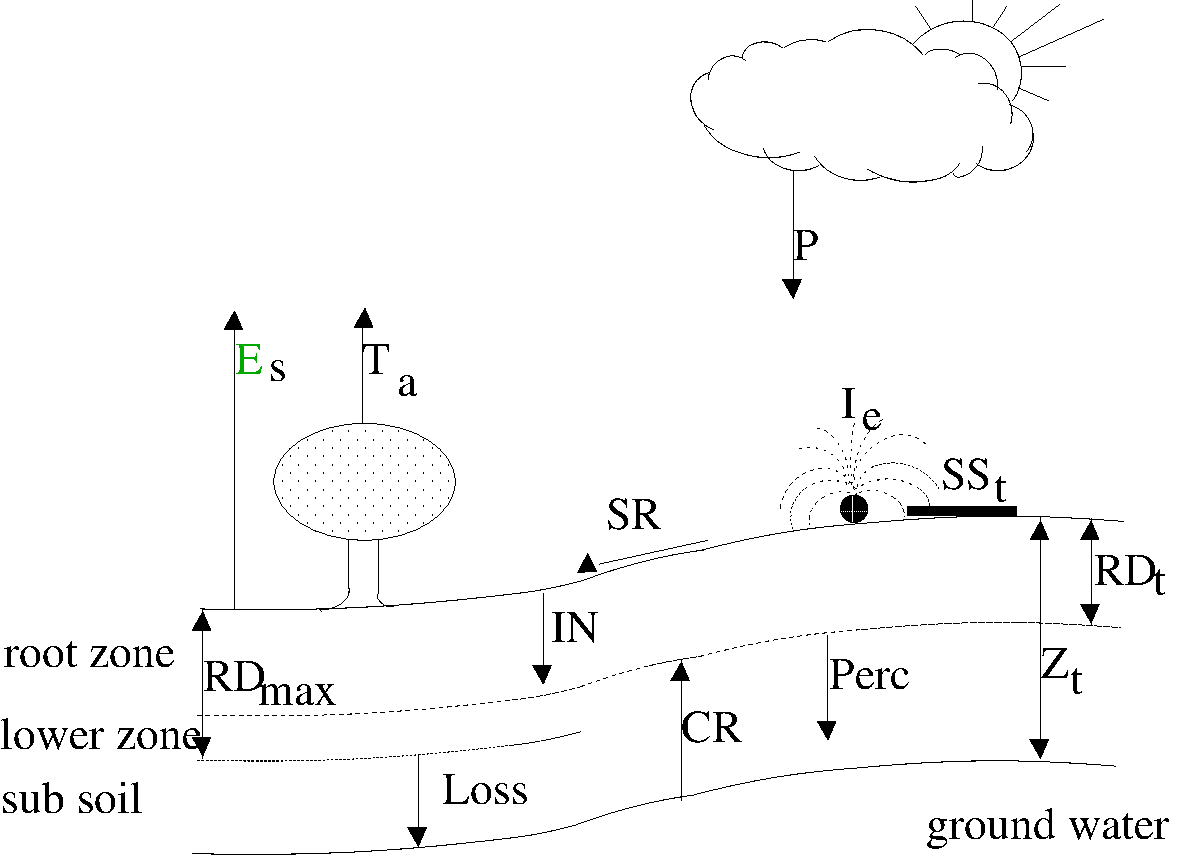
\includegraphics[width=120mm]{\FigDir/WATBAL1.pdf}
\caption{Schematic representation of the different components of a soil water balance}
\label{fig:WatBalSchematic}
\end{figure}

The actual soil moisture content can be established according to (Driessen, 1986):

\stepcounter{equation}
\begin{align}
% equations 6.1a-b
\label{eq:6.1}
\theta_{t~} &= {\frac{IN _{up} ~+~(IN _{low} ~-~T _{a} )}{RD}} \Delta t \subeqn \\[1em]
IN_{up} &= P~+~I _{e} ~-~E _{s} ~+~SS _{t} \, /\Delta t-~SR  \subeqn  \\[1em]
IN_{low} &= CR~-~Perc \subeqn
\end{align}

Where:\\[5pt]
\begin{tabularx}{\textwidth}{llXr}
$\theta$$_{{\rm t}}$ &:& Actual moisture content of the root zone at time step t
   & [cm$^{{\rm 3}}$ cm$^{{\rm -3}}$]\\
IN$_{{\rm up}}$ &:& Rate of net influx through the upper root zone boundary
   & [cm d$^{{\rm -1}}$]\\
IN$_{{\rm lo}}$$_{{\rm w}}$ &:& Rate of net influx through the lower root zone boundary
   & [cm d$^{{\rm -1}}$]\\
T$_{{\rm a}}$ &:& Actual transpiration rate of crop
   & [cm d$^{{\rm -1}}$]\\
RD &:& Actual rooting depth  & [cm]\\
P &:& Precipitation intensity  & [cm d$^{{\rm -1}}$]\\
I$_{{\rm e}}$ &:& Effective daily irrigation  & [cm d$^{{\rm -1}}$]\\
E$_{{\rm s}}$ &:& Soil evaporation rate   & [cm d$^{{\rm -1}}$]\\
SS$_{{\rm t}}$ &:& Surface storage  & [cm]\\
SR &:& Rate of surface runoff  & [cm d$^{{\rm -1}}$]\\
CR &:& Rate of capillary rise  & [cm d$^{{\rm -1}}$]\\
Perc &:& Percolation rate  & [cm d$^{{\rm -1}}$]\\
$\Delta$t &:& Time step  & [d]\\
Z$_{{\rm t}}$ &:& Depth of groundwater table (see figure \ref{fig:WatBalSchematic})  & [cm]\\
\end{tabularx}

Processes directly affecting soil moisture content of the root zone can be defined as:
\begin{itemize}
\item infiltration is transport from the soil surface into the root zone;
\item evaporation is the loss of soil moisture to the atmosphere;
\item transpiration by plants is loss of water from the interior root zone;
\item percolation is downward transport of water from the root zone to the layer below the root zone;
\item capillary rise is upward transport into the rooted zone.
\end{itemize}

The water balance equation has to be solved for each time interval in the crop growth cycle.

In the model the soil water balance calculations for potential production and the soil water
balance calculations for water limited production have been separated into different
subroutines. For the calculation of potential production the soil moisture content is
assumed to be at field capacity and no calculations have to be performed to simulate the
water balance in the soil. Only the actual evaporation rate and the actual transpiration rate
have to be accumulated. 

For the calculation of the water limited production two different soil water balances are
distinguished. One soil water balance without groundwater influence (i.e. for a freely
draining soil) and one soil water balance with groundwater influence. In the JRC version
of WOFOST, the system with groundwater is not activated because of lack of sufficiently
good data. However, the groundwater option can be easily applied whenever data are
made available. So, actually three water balance subroutines can be distinguished:
\begin{itemize}
\item Potential production [WATPP, \S \ref{sec:WATPP}]
\item Water limited production, without groundwater influence [WATFD, \S \ref{sec:WATFD}]
\item Water limited production, with groundwater influence [WATGW, \S \ref{sec:WATGW}]
\end{itemize}

The actual transpiration rate of a canopy, used in the calculations of potential and water
limited production, is calculated in the same way for all options. The calculation method
will therefore be treated separately in \S \ref{sec:evapotranspiration}. 

The capillary rise in the system with groundwater influence is a complicated subject. It
will be discussed separately in \S \ref{sec:CapillaryFlow}.

In the calculations for the water limited growth the water content of the root zone is the
most important state variable. In- and outflow of water is calculated for each time step. It
is important to realize that the model is not intended for detailed physical treatment of
water movement in the soil, but only for estimating moisture availability to the crop. The
distribution of water within the root zone is assumed to be instantaneous (within the time
step of the model, being one day). The available water contained in the rooted zone is
directly at the disposal of the crop. Water just below the root zone is available after
further root growth and water below the potential rooting depth cannot be used by the
crop.

The process of infiltration is not treated in a physical sense at all, because simulation of
this process would require a much smaller time step (Rietveld, 1978; Stroosnijder {\it et al}.,
1972; van Keulen \& van Beek, 1971). Instead a predefined fraction of the rain is not
infiltrating on the day of rainfall (van Diepen {\it et al}., 1988).

Soil water content at saturation is equal to soil porosity. Field capacity is the volumetric
water content of the soil after wetting and initial redistribution (Veihmeyer \& Hendrickson, 
1931). It is often treated as a soil characteristic (van Keulen, 1975; Driessen, 1986;
Jansen \& Gosseye, 1986), although it also depends on boundary conditions. Field capacity
is usually defined as the volumetric  water content at a soil moisture suction of 100 mbar
or pF 2.0 at least in the Netherlands. It is the moisture suction in equilibrium with a
groundwater table at 100 cm. Elsewhere in the world, for loamy soils field capacity
corresponds with a value of 200 mbar moisture suction. For sandy soils 60 mbar is a
realistic value under field conditions. Above a certain value of moisture suction, plants do
not recover and wilt permanently. The volumetric water content of the soil at this point is
called wilting point. The soil moisture at wilting point has usually a value of about 16000
mbar or pF 4.2. The soil moisture content of an air dry soil is assumed to be at pF 7.0
(van Keulen, 1975).

\section{Evapo(transpi)ration}
\label{sec:evapotranspiration}

In the subroutine {\bf EVTRA} the following processes are calculated for a given crop cover:
\begin{itemize}
\item The maximum evaporation rate from a shaded soil surface;
\item The maximum evaporation rate from a shaded water surface;
\item The maximum crop transpiration rate;
\item The actual crop transpiration rate. 
\end{itemize}

Transpiration, or the rate of water loss from the plants depends on the energy available
for vaporization, on the difference in vapor pressure between the plant and the surrounding 
air and on the resistance to water vapor diffusion from the stomatal cavity to the
atmosphere (van Keulen \& Seligman, 1987). Potential transpiration is the water loss from
a field crop which covers the soil completely and has an optimum supply of water from
the soil. The method, introduced by Penman (1956, 1948) and for the present use,
adapted according to Choisnel {\it et al}. (1992), is now used for daily totals of canopy
transpiration and for daily totals of soil evaporation (Jarvis, 1981; Feddes {\it et al}., 1978;
van Keulen, 1975)

\subsection{Evaporation and transpiration}
Potential evapotranspiration of a crop ET0 is the sum of potential transpiration T$_{{\rm m}}$ and
soil evaporation E0$_{{\rm s}}$.

\begin{equation}
\label{eq:6.2}
ET0 ~=~ E0_{s} ~+~ T_{m} 
\end{equation}
 
Where:\\[5pt]
\begin{tabularx}{\textwidth}{llXr}
ET0 &:& Potential evapotranspiration rate (see \S 4.1.3) & [cm d$^{{\rm -1}}$]\\
E0$_{{\rm s}}$ &:& Potential evaporation of a bare soil (see \S 4.1.3)  & [cm d$^{{\rm -1}}$]\\
T$_{{\rm m}}$ &:& Maximum crop transpiration rate (see eq. 6.4)  & [cm d$^{{\rm -1}}$]\\
\end{tabularx}

For some crops the potential evapotranspiration can be higher than the Penman evapotranspiration. 
Therefore, in the model a correction factor, a so called  crop coefficient
(acronym: {\bf CFET}) is introduced to account for this effect. The Penman evapotranspiration
should be multiplied by this crop coefficient (Feddes, 1978; Doorenbos \& Pruitt, 1977).
The evaporation is reduced due to the presence of vegetation, which intercepts the solar
energy and reduces the windspeed. The evaporation of the soil as a function of the leaf
area index (Goudriaan, 1977; Ritchie, 1972; 1971) can be estimated as:

\begin{equation}
\label{eq:6.3}
E0 _{s} ~=~ ET0 \cdot e^{-\kappa_{gb} \cdot LAI}
\end{equation}

Where:\\[5pt]
\begin{tabularx}{\textwidth}{llXr}
E0$_{{\rm s}}$ &:& Potential bare soil evaporation  & [cm d$^{{\rm -1}}$]\\
 $\kappa$$_{{\rm gb}}$ &:& Extinction coefficient for global radiation  & [-]\\
 LAI &:& Leaf area index  & [ha ha$^{{\rm -1}}$]\\
\end{tabularx}
 
The potential transpiration rate can be calculated by combining equations \ref{eq:6.2} and 
\ref{eq:6.3}.

\begin{equation}
\label{eq:6.4}
T _{m} ~=~ ET0\, (1~-~e ^{-\kappa _{gb} \, LAI} )
\end{equation}
 
Where:\\[5pt]
\begin{tabularx}{\textwidth}{llXr}
T$_{{\rm m}}$ &:& Maximum crop transpiration rate & [cm d$^{{\rm -1}}$]\\
ET0 &:& Potential evapotranspiration rate & [cm d$^{{\rm -1}}$]\\
$\kappa$$_{{\rm gb}}$ &:& Extinction coefficient for global radiation & [-]\\
LAI &:& Leaf area index (see \S \ref{sec:5.4.5}) & [ha ha$^{{\rm -1}}$]\\
\end{tabularx}

The extinction coefficient for global radiation can be estimated as a factor times the
extinction coefficient of diffuse radiation:

\begin{equation}
\label{eq:6.5}
\kappa_{gb} ~=~ 0.75\, \kappa_{df} 
\end{equation}

Where:\\[5pt]
\begin{tabularx}{\textwidth}{llXr}
$\kappa_{{\rm gb}}$ &:& Extinction coefficient for global radiation & [-]\\
$\kappa_{{\rm df}}$ &:& Extinction coefficient for diffuse light & [-]\\
\end{tabularx}

The maximum evaporation rate from a shaded water surface can be calculated in the same
way as equation \ref{eq:6.4}: 

\begin{equation}
\label{eq:6.6}
E_{w,\max } ~=~ E0_{w} \cdot e^{-\kappa_{gb} LAI}
\end{equation}

Where:\\[5pt]
\begin{tabularx}{\textwidth}{llXr}
E$_{{\rm w,max}}$ &:& Maximum evaporation rate from a shaded water surface & 
    [cm d$^{{\rm -1}}$]\\
E0$_{{\rm w}}$ &:& Potential evaporation rate from a water surface 
    (see \S \ref{sec:penman}) & [cm d$^{{\rm -1}}$]\\
$\kappa$$_{{\rm gb}}$ &:& Extinction coefficient for global radiation & [-]\\
LAI &:& Leaf area index & [ha ha$^{{\rm -1}}$]\\
\end{tabularx}

The maximum evaporation rate from a shaded bare soil surface can also be calculated in
the same way as in equation \ref{eq:6.4} and \ref{eq:6.6}:

\begin{equation}
\label{eq:6.7}
E_{s,\max } ~=~ E0 _{s} \,\,\, e ^{-\kappa  _{gb} LAI}
\end{equation}

Where:\\[5pt]
\begin{tabularx}{\textwidth}{llXr}
E$_{{\rm s,max}}$ &:& Maximum evaporation rate from a shaded 
    soil surface & [cm d$^{{\rm -1}}$]\\
E0$_{{\rm s}}$ &:& Potential evaporation rate from a bare soil 
    surface & [cm d$^{{\rm -1}}$]\\
$\kappa$$_{{\rm gb}}$ &:& Extinction coefficient for total global radiation & [-]\\
LAI &:& Leaf area index & [ha ha$^{{\rm -1}}$]\\
\end{tabularx}

\subsection{Reduction of the transpiration due to water stress}

For the potential run the actual transpiration rate is always equal to the maximum
transpiration rate, because sufficient water is available. The actual transpiration rate is
calculated from the maximum transpiration rate, taking into account reductions for
shortage or excess of water in the root zone. Water uptake by the roots depends on the
difference in potential between the water in the plant and in the soil, and on the resistance
to transport of moisture from the soil to the atmosphere (van Keulen \& Seligman, 1987).
In contrast to Feddes {\it et al}. (1978) not soil water potential, but soil water content is
chosen as the independent variable (Gollan {\it et al}., 1986; Schulze 1986).

Up to a point, the water potential in the plant can be adapted in order to maintain
potential transpiration. At what soil moisture content the transition from potential
transpiration to a transpiration deficit takes place, is difficult to quantify. In the model,
the actual transpiration for the water limited run is obtained by multiplying the potential
transpiration with a reduction factor. This reduction factor is defined as (van Diepen {\it et
al}., 1988):

\begin{equation}
\label{eq:6.8}
R_{ws} ~=~{\frac{\theta_{t} ~-~ \theta  _{wp} }{ \ _{ws} ~-~ \theta_{wp} }}
\end{equation}

Where:\\[5pt]
\begin{tabularx}{\textwidth}{llXr}
$R_{{\rm ws}}$ &:& Reduction factor for transpiration in case of
    water shortage & [-]\\
$\theta_{{\rm t}}$ &:& Actual soil moisture content (see eq. 6.1 and 
    6.34) & [cm$^{{\rm 3}}$ cm$^{{\rm -3}}$]\\
$\theta_{{\rm wp}}$ &:& Soil moisture content at wilting 
    point & [cm$^{{\rm 3}}$ cm$^{{\rm -3}}$]\\
$\theta_{{\rm ws}}$ &:& Critical soil moisture & [cm$^{{\rm 3}}$ cm$^{{\rm -3}}$]\\ 
\end{tabularx}

The critical soil moisture content is defined as the quantity of stored soil moisture below
which water uptake is impaired and the crop begins to close its stomata. It is not a fixed
value. Restriction of water uptake due to water stress starts at a higher water content
when the potential transpiration rate is higher (Denmead \& Shaw, 1962). The critical
moisture content can be calculated as (van Diepen {\it et al}., 1988):

\begin{equation}
\label{eq:6.9}
\theta_{ws} ~=~ (1\, -\, p )\, (\theta_{fc} \, -\, \theta_{wp} )\, +\, \theta_{wp} 
\end{equation}

Where:\\[5pt]
\begin{tabularx}{\textwidth}{llXr}
$\theta$$_{{\rm ws}}$ &:& Critical soil moisture content & [cm$^{{\rm 3}}$ cm$^{{\rm -3}}$]\\
p &:& Soil water depletion fraction as a function 
     of pot. evapotranspiration & [cm$^{{\rm 3}}$ cm$^{{\rm -3}}$]\\
$\theta$$_{{\rm fc}}$ &:& Soil moisture content at field capacity & [cm$^{{\rm 3}}$ cm$^{{\rm -3}}$]\\
$\theta$$_{{\rm wp}}$ &:& Soil moisture content at wilting point & [cm$^{{\rm 3}}$ cm$^{{\rm -3}}$]\\
\end{tabularx}

The soil moisture content at field capacity, {\bf $\theta$$_{{\rm fc}}$} (acronym: {\bf SMFCF}), 
and the soil moisture content at wilting point, {\bf $\theta$$_{{\rm wp}}$} (acronym: {\bf SMW}), 
are soil specific and should be given by the user. The soil water depletion fraction, p, is 
a function of the potential evapotranspiration rate (for a closed canopy) and the crop group 
number. It is established in subroutine
{\bf SWEAF}. In literature, instead of the term soil water depletion fraction, also the 
expression easily available water is used. Easily available water is defined as the amount of
water between $\theta$$_{{\rm fc}}$ and $\theta$$_{{\rm wp}}$ which can be extracted from the root 
zone without reducing the
transpiration. Indicative p-values for the most important crops at different values of ET0
are presented in Table 6.1. The crop group number ranges from 1 (drought-sensitive) to 5
(drought-resistant). An example of a classification of the different crop groups is
presented in Table 6.2.

\begin{table}
% Table 6.1
\caption{Soil water depletion fraction (p) as a function of potential evapotranspiration 
of a closed crop canopy for different crop groups (Doorenbos {\it et al}.,1978).}
\label{tbl:soilwatdeplfraction}
\begin{tabularx}{\textwidth}{Xrrrrrrrrr}
\hline
\multicolumn{10}{c}{Crop ET0 in cm d-1}\\
\hline
group$^{\rm *}$ & 0.2 & 0.3 & 0.4 & 0.5 & 0.6 & 0.7 & 0.8 & 0.9 & 1.0\\
1 & 0.45 & 0.38 & 0.30 & 0.25 & 0.23 & 0.20 & 0.18 & 0.16 & 0.15\\
2 & 0.60 & 0.50 & 0.43 & 0.35 & 0.30 & 0.28 & 0.25 & 0.23 & 0.20\\
3 & 0.75 & 0.65 & 0.55 & 0.45 & 0.40 & 0.38 & 0.33 & 0.30 & 0.25\\
4 & 0.85 & 0.75 & 0.65 & 0.55 & 0.50 & 0.48 & 0.43 & 0.38 & 0.35\\
5 & 0.92 & 0.85 & 0.75 & 0.65 & 0.60 & 0.55 & 0.50 & 0.48 & 0.45\\
\hline 
\end{tabularx} 
\end{table}


\begin{table}
% Table 6.2
\caption{Example of crops in the different crop groups (Doorenbos {\it et al}., 1978).}
\label{tbl:ExampleCropGroups}
\begin{tabularx}{\textwidth}{lX}
\hline
Group no & Representative crop types\\
\hline
1 & leaf vegetables, strawberry\\     
1-2 & cabbage, onion\\
2 & clover, carrot, early tobacco\\     
2-3 & banana, pepper\\
3 & grape, pea, potato\\
3-4 & bean, sunflower, tomato, water melon, grass\\
4 & citrus, groundnut, pineapple\\
4-5 & alfalfa cotton, tobacco, cassava, sweet potato, grains\\
5 & olive, safflower, sorghum, soybean, sugarcane\\
\hline
\end{tabularx}
\end{table}

The soil water depletion fraction for very high values of potential evapotranspiration of a
closed canopy can be as low as 0.10. For very low values of potential evapotranspiration
of a closed canopy this fraction can be as high as 0.96.
Note that it is possible that the reduction factor R$_{{\rm ws}}$ (eq. \ref{eq:6.8}) might obtain 
values higher
than unity and lower than zero for certain values of p and $\theta$$_{{\rm t}}$. Since this does not make
any sense, in the model the highest possible value for R$_{{\rm ws}}$ is set to unity and the lowest
possible value is set to zero.
An empirical formula can be used to calculate the fraction of easily available soil water,
yielding identical values as the ones given in the Table \ref{tbl:soilwatdeplfraction} 
(van Diepen {\it et al}., 1988).

\begin{equation}
\label{eq:6.10}
p~={\frac{~1}{ \alpha _{p} ~+~ \beta _{p} ~ET0}} ~-~ 0.10\, (\, 5~-~No _{cg} \, )
\end{equation}

Where:\\[5pt]
\begin{tabularx}{\textwidth}{llXr}
p &:& Fraction of easily available soil water  & [cm$^{{\rm 3}}$ cm$^{{\rm -3}}$]\\
$\alpha$$_{{\rm p}}$ &:& Regression constant {\small (=0.76 van Diepen et al., 1988)}  & [-]\\
$\beta$$_{{\rm p}}$ &:& Regression constant {\small (=1.5 van Diepen et al., 1988)}  & [d cm-$^{{\rm 1}}$]\\
ET0 &:& Potential evapotranspiration rate  & [cm d$^{{\rm -1}}$]\\
No$_{{\rm cg}}$ &:& Crop Group number {\small (=1 to 5, Doorenbos et al., 1978)}  & [-]\\
\end{tabularx}
 
Note that crop group number, {\bf No$_{{\rm cg}}$} (acronym: {\bf DEPNR}) is input in the model and should
be provided by the user.

For crop group 1 and 2 this estimate is not very accurate and an additional correction is
applied to reproduce the table values correctly (van Diepen {\it et al}., 1988):

\begin{equation}
%eq 6.11
p~=~p~+~{\frac{ET0 ~-~ 0.6}{No _{cg} \, (\, No _{cg} ~+~3\, )}}
\end{equation}

Where:\\[5pt]
\begin{tabularx}{\textwidth}{llXr}
where p &:& Fraction of easily available soil water  & [cm$^{{\rm 3}}$ cm$^{{\rm -3}}$]\\
ET0 &:& Potential evapotranspiration rate  & [cm d$^{{\rm -1}}$]\\
No$_{{\rm cg}}$ &:& Crop Group number {\small (=1 to 5, Doorenbos et al., 1978)}  & [-]\\
\end{tabularx}

\subsection{Reduction of the transpiration due to oxygen stress}
The transpiration rate of the plants can also be reduced when the root zone is completely
saturated. Root systems which have been developed in aerobic soils do not have airducts
and degenerate within several days when anaerobic conditions (waterlogging) are imposed
(Penning de Vries {\it et al}., 1989). Flooding quickly depletes the O$_{{\rm 2}}$ in the soil and root cells
disintegrate when their metabolic activities are hampered by oxygen depletion. For
detailed information on the physiological effects of excess water on a crop see Jackson
and Drew (1984).

Reduction in transpiration occurs when the actual soil moisture content exceeds the
critical soil moisture content for aeration. The critical soil moisture content for aeration
can be calculated as:

\begin{equation}
\label{eq:6.12}
\theta_{air} ~=~ \theta_{\max} ~-~\theta_{c} 
\end{equation}

Where:\\[5pt]
\begin{tabularx}{\textwidth}{llXr}
$\theta$$_{{\rm air}}$ &:& Critical soil moisture content for aeration & [cm$^{{\rm 3}}$ cm$^{{\rm -3}}$]\\
$\theta$$_{{\rm max}}$ &:& Soil porosity & [cm$^{{\rm 3}}$ cm$^{{\rm -3}}$]\\
$\theta$$_{{\rm c}}$ &:& Critical air content & [cm$^{{\rm 3}}$ cm$^{{\rm -3}}$]\\
\end{tabularx}

The soil porosity, {\bf $\theta$$_{{\rm max}}$} (acronym: {\bf SMO}) and the critical soil air 
content, {\bf $\theta$$_{{\rm c}}$} (acronym:{\bf CRAIRC}), are soil specific and should 
be provided by the user. 

In the model, maximum reduction is reached after four successive days of anaerobic
conditions. In reality however, this period depends on the development stage and on the
species. If at the fifth successive day oxygen shortage occurs the reduction remains the
same as on the fourth day. The reduction factor for the transpiration rate due to oxygen
shortage can be calculated as (van Diepen, personal communication):

\stepcounter{equation}
\begin{align}
\label{eq:6.13a-b}
R_{os,\max } &= \frac{ \theta  _{\max } ~-~ \theta  _{t} }{\theta _{\max } ~-~ \theta  _{air} } \subeqn  \\
R_{os} &= 1 - \frac{No _{d} }{4} \, (\, 1\, -\, R _{os,\max } \, ) ~~~ with~~ No_{d} ~\le ~ 4 \subeqn
\end{align}

Where:\\[5pt]
\begin{tabularx}{\textwidth}{llXr}
 R$_{{\rm os,max}}$ &:& Maximum reduction factor due to oxygen shortage & [-]\\
 R$_{{\rm os}}$ &:& Reduction factor due to oxygen shortage & [-]\\
 $\theta$$_{{\rm air}}$ &:& Critical soil moisture content for aeration 
     & [cm$^{{\rm 3}}$ cm$^{{\rm -3}}$]\\
 $\theta$$_{{\rm max}}$ &:& Soil porosity & [cm$^{{\rm 3}}$ cm$^{{\rm -3}}$]\\
 $\theta$$_{{\rm t}}$ &:& Actual soil moisture content (see eq. \ref{eq:6.34}) 
     & [cm$^{{\rm 3}}$ cm$^{{\rm -3}}$]\\
 No$_{{\rm d}}$ &:& Number of successive days with oxygen stress & [-]\\
\end{tabularx}

For crops which roots develop airducts, like for example rice, and for crops grown on
perfectly drained land, the reduction factor for oxygen shortage equals unity. If this ratio
is less then unity, the actual transpiration rate is reduced proportionally.

Usually, in freely draining soils oxygen stress does not play any role. It may occur when
the critical soil moisture content for aeration is greater than the soil moisture content at
field capacity and when the subsoil is very slowly permeable. In case of groundwater
influence, oxygen shortage may occur regularly. However, the process of transpiration
reduction due oxygen shortage is poorly parametrized and therefore values for the
reduction factor are rather speculative. 

\subsection{Actual transpiration}
As a result of water excess and/or water shortage the actual transpiration rate can be
calculated as:

\begin{equation}
\label{eq:6.14}
T_{a~} = R_{ws} \,\, R_{os} \,\, T_{m} 
\end{equation}

Where:\\[5pt]
\begin{tabularx}{\textwidth}{llXr}
 T$_{{\rm a}}$ &:& Actual transpiration rate & [cm d$^{{\rm -1}}$]\\
 T$_{{\rm m}}$ &:& Maximum transpiration rate (see eq. \ref{eq:6.4}) & [cm d$^{{\rm -1}}$]\\
 R$_{{\rm os}}$ &:& Reduction factor due to oxygen reduction & [-]\\
 R$_{{\rm ws}}$ &:& Reduction factor due to water shortage (see eq. \ref{eq:6.8}) & [-]\\
\end{tabularx}
 
\section{Soil water balance calculations, potential production}
\label{sec:WATPP}

In the subroutine {\bf WATPP}, the variables of the soil water balance in the potential 
production situation are calculated. The purpose is to quantify the crop water requirements for
continuous growth without drought stress. It is assumed that the soil is permanently at
field capacity.

\begin{equation}
\label{eq:6.15}
\theta  _{t} ~ =~\theta  _{fc} 
\end{equation}

Where:\\[5pt]
\begin{tabularx}{\textwidth}{llXr}
 $\theta$$_{{\rm t}}$ &:& Actual soil moisture content & [cm$^{{\rm 3}}$ cm$^{{\rm -3}}$]\\
 $\theta$$_{{\rm fc}}$ &:& Soil moisture content at field capacity & [cm$^{{\rm 3}}$ cm$^{{\rm -3}}$]\\
\end{tabularx}
 
Rainfall, irrigation, capillary rise and drainage are not taken into account. This does not
mean that these processes will not occur. The result of these processes will be a soil
moisture content at field capacity level. The only two processes to consider are evaporation of 
the surface and the transpiration of the crops. In the previous paragraph the
calculation of these processes is described in detail.

The evaporation rate is calculated for two situations. In the first situation
Airducts are present in the roots. This means that the crop tolerates waterlogging. This
is the case for example with rice. The evaporation rate is then calculated as the 
evaporation rate from a shaded water surface:

\begin{equation}
%eq 6.16
E _{w} ~=~ E _{w, \max } 
\end{equation}

Where:\\[5pt]
\begin{tabularx}{\textwidth}{llXr}
    E$_{{\rm w}}$ &:& Evaporation rate from a shaded water surface & [cm d$^{{\rm -1}}$]\\
    E$_{{\rm w,max}}$ &:& Maximum evaporation rate from shaded 
    water surface (see eq. \ref{eq:6.6}) & [cm d$^{{\rm -1}}$]\\
\end{tabularx}

In the second situation airducts are absent in the roots. This means that the crop does
not tolerate water
logging. This is the case for most crops. The evaporation rate is then calculated as the
evaporation rate from a soil surface (van Diepen, personal communication):  

\begin{equation}
\label{eq:6.17}
E _{s~} =~ E _{s,\max } {\frac{ \theta  _{fc} ~-~ {{\frac{\theta  _{wp} }{3}}} }{\theta  _{\max } ~-~{{\frac{\theta  _{wp} }{3}}} }}
\end{equation}

Where:\\[5pt]
\begin{tabularx}{\textwidth}{llXr}
    E$_{{\rm s}}$ &:& Evaporation rate from a shaded soil surface & [cm d$^{{\rm -1}}$]\\
    E$_{{\rm s,max}}$ &:& Maximum evaporation rate from a shaded
    soil surface (see eq. \ref{eq:6.7}) & [cm d$^{{\rm -1}}$]\\
    $\theta$$_{{\rm fc}}$ &:& Soil moisture content at field capacity & [cm$^{{\rm 3}}$ cm$^{{\rm -3}}$]\\
    $\theta$$_{{\rm wp}}$ &:& Soil moisture content at wilting point & [cm$^{{\rm 3}}$ cm$^{{\rm -3}}$]\\
    $\theta$$_{{\rm max}}$ &:& Soil porosity & [cm$^{{\rm 3}}$ cm$^{{\rm -3}}$]\\
\end{tabularx}

\section{System without groundwater influence}
\label{sec:WATFD}

In the subroutine {\bf WATFD}, the variables of the soil water balance in the actual 
water-limited production situation are calculated for freely draining soil. No influence from
groundwater is assumed. The purpose is to quantify the crop water requirements for
continuous growth with either drought stress or water excess, and to quantify a possible
reduction of the crop transpiration rate, leading to a reduced growth.

\subsection{The soil water submodel}

For the rooted zone the water balance equation is solved every daily time step. At the
upper boundary, processes comprise the infiltration of water from precipitation or
irrigation, evaporation from the soil surface and uptake of water and transpiration by the
crop. If rainfall intensity exceeds the infiltration and surface storage capacity of the soil,
water runs off. Water can be stored in the soil till the field capacity is reached. Additional
water percolates beyond the lower boundary of the rooting zone.
The flow rates are limited by the maximum percolation rate of the root zone and the
maximum percolation rate of the water to the subsoil.

The textural profile of the soil is conceived homogeneous. Initially the soil profile
consists of three layers (zones):
\begin{itemize}
\item the rooted zone between soil surface and actual rooting depth
\item the lower zone between actual rooting depth and maximum rooting depth
\item the subsoil below maximum rooting depth
\end{itemize}

The extension of the root zone from initial rooting depth to maximum rooting depth is
described in \S \ref{sec:rootgrowth}. Its effect on the soil moisture content is accounted 
for in this soil water
balance calculation. From the moment that the maximum rooting depth is reached the soil
profile is described as a two layer system (Driessen, 1986). The lower zone no longer
exists.

The water balance is driven by rainfall, possibly buffered as surface storage, and
evapotranspiration. The processes considered are infiltration, soil water retention,
percolation and the loss of water beyond the maximum root zone.

As mentioned earlier, no groundwater influence is assumed, therefore capillary rise is not
accounted for. Only downward flow, evaporation from the soil surface and transpiration
are included in the calculations. 

\subsection{Elements of the water balance  }
\label{sec:WBElements}

\subsubsection{Initial soil water content and initial soil water amount}

The initial value of the actual soil moisture content in the rooted part of the soil can be
calculated as:

\begin{equation}
\label{eq:6.18}
\theta_{t} ~ =~\theta_{wp} ~+~{\frac{W_{av}}{RD}}
\end{equation}

Where:\\[5pt]
\begin{tabularx}{\textwidth}{llXr}
$\theta$$_{{\rm t}}$ &:& Actual soil moisture content in rooted z
    one  & [cm$^{{\rm 3}}$ cm$^{{\rm -3}}$]\\
$\theta$$_{{\rm wp}}$ &:& Soil moisture content at wilting   & [cm$^{{\rm 3}}$ cm$^{{\rm -3}}$]\\
W$_{{\rm av}}$ &:& Initial amount of available soil moisture 
    in excess of $\theta$$_{{\rm wp}}$ & [cm]\\
RD &:& Actual rooting depth (see \S 5.5) & [cm]\\
\end{tabularx}

It should be mentioned that the initial actual soil moisture content, $\theta$$_{{\rm t}}$, cannot be lower
than the soil moisture content at wilting point. In case the crop cannot develop airducts,
the initial soil moisture content cannot be higher than the soil moisture content at field
capacity. If the crop can develop airducts the initial soil moisture content cannot exceed
the soil porosity. {\bf W$_{{\rm av}}$} (acronym: {\bf WAV}), the initial amount of available 
soil moisture in excess of $\theta$$_{{\rm wp}}$ should be provided by the user. 

Multiplying the actual soil moisture content with the rooting depth yields the initial
amount of water in the rooted zone. The initial amount of soil moisture in the lower zone,
the zone between the rooted zone and the maximum rooting depth, can be calculated as:

\begin{equation}
\label{eq:6.19}
W_{lz} ~ =~ W _{av} ~+~ RD_{\max } ~\theta_{wp} ~-~RD~\theta_{t} 
\end{equation}

Where:\\[5pt]
\begin{tabularx}{\textwidth}{llXr}
 W$_{{\rm lz}}$ &:& Amount of soil moisture in the lower zone & [cm]\\
 W$_{{\rm av}}$ &:& Initial amount of available soil moisture 
    in excess of $\theta$$_{{\rm wp}}$ & [cm]\\
 RD$_{{\rm max}}$ &:& Maximum rooting depth & [cm]\\
 RD &:& Actual rooting depth & [cm]\\
 $\theta$$_{{\rm t}}$ &:& Actual soil moisture content in rooted zone  
     & [cm$^{{\rm 3}}$ cm$^{{\rm -3}}$]\\
 $\theta$$_{{\rm wp}}$ &:& Soil moisture content at wilting point  
     & [cm$^{{\rm 3}}$ cm$^{{\rm -3}}$]\\
\end{tabularx}

The soil moisture content of the lower zone is also limited by the field capacity in case
the crop cannot develop airducts, else the soil moisture content is limited by the soil
porosity. In the model, initially, the variable D$_{{\rm slr}}$, days since last rain, is set 
to one. If the
actual soil moisture content is halfway between the field capacity and wilting point a
value of five days is assumed. 

\subsubsection{Evaporation}

The evaporation rate is computed by the soil water balance as it is independent of whether
a crop is present on the soil surface or not.

The evaporation depends on the amount of available water in the soil and the infiltration
capacity of the soil. If the water layer on the surface, the so called surface storage, 
exceeds 1 cm, the actual evaporation rate from the soil is set to zero and the actual
evaporation rate from the surface water is equal to the maximum evaporation from a
shaded water surface.

If the surface storage is less than 1 cm and the infiltration rate of the previous day
exceeds 1 cm d$^{{\rm -1}}$, the actual evaporation rate from the surface water is set to zero and the
actual evaporation rate from the soil is equal to the maximum evaporation from a shaded
soil surface. All water on the surface can infiltrate within one day. The value of the
variable days since last rain, D$_{{\rm slr}}$, is reset to unity.

If the infiltration rate is less than 1 cm d$^{{\rm -1}}$, the amount of infiltrated water is considered
too small to justify a reset of the parameter D$_{{\rm slr}}$ and the evaporation rate decreases as the
top soil starts drying. The reduction of the evaporation is thought to be proportional to the
square root of time (Stroosnijder, 1987, 1982). The evaporation can be calculated as:

\begin{equation}
\label{eq:6.20}
E _{s} ~=~ E _{s,\max } ( \sqrt{D _{slr} } ~-~ \sqrt{D _{slr} \, -\, 1} )
\end{equation}

Where:\\[5pt]
\begin{tabularx}{\textwidth}{llXr}
E$_{{\rm s}}$ &:& Evaporation rate from a shaded soil surface  & [cm d$^{{\rm -1}}$]\\
E$_{{\rm s,max}}$ &:& Maximum evaporation rate from a shaded soil
   surface (see eq. \ref{eq:6.7})  & [cm d$^{{\rm -1}}$]\\
D$_{{\rm slr}}$ &:& Days since last rain  & [d]\\
\end{tabularx}

When a small amount of water has infiltrated, or rather wetted the soil surface, this
amount can be evaporated the same day, irrespective of D$_{{\rm slr}}$. Therefore, the actual
evaporation from the soil surface, as calculated according to equation \ref{eq:6.20}, should be
corrected for this amount of water infiltrating the soil. This amount should be added to
the actual evaporation rate. However, it should be noted that the actual evaporation never
can exceed the maximum evaporation rate.

\subsubsection{Precipitation}
Not all the precipitation will reach the surface. A fraction will be intercepted by leaves,
stems, etc. From the amount of precipitation which reaches the soil surface, not all will
infiltrate. A part runs off. Runoff from a field can be 0-20 percent, and even higher on
unfavorable surfaces (Stroosnijder \& Kon\'{e}, 1982). In the model, it is assumed that a
fixed fraction of the precipitation will not infiltrate on the same day. This fraction can be
reduced in situations with relatively small amounts of rainfall. In the model a reduction
factor is defined as function of the amount of rainfall (van Diepen {\it et al}., 1988). See 
figure \ref{fig:NonInfiltFrac} and equation \ref{eq:6.26}. Note that the non infiltrating 
fraction refers to rainfall only.
Irrigation water is assumed to infiltrate freely. However, the irrigation option is not
implemented in WOFOST 6.0.

\begin{figure}[p]
% Fig. 6.2 
\centering
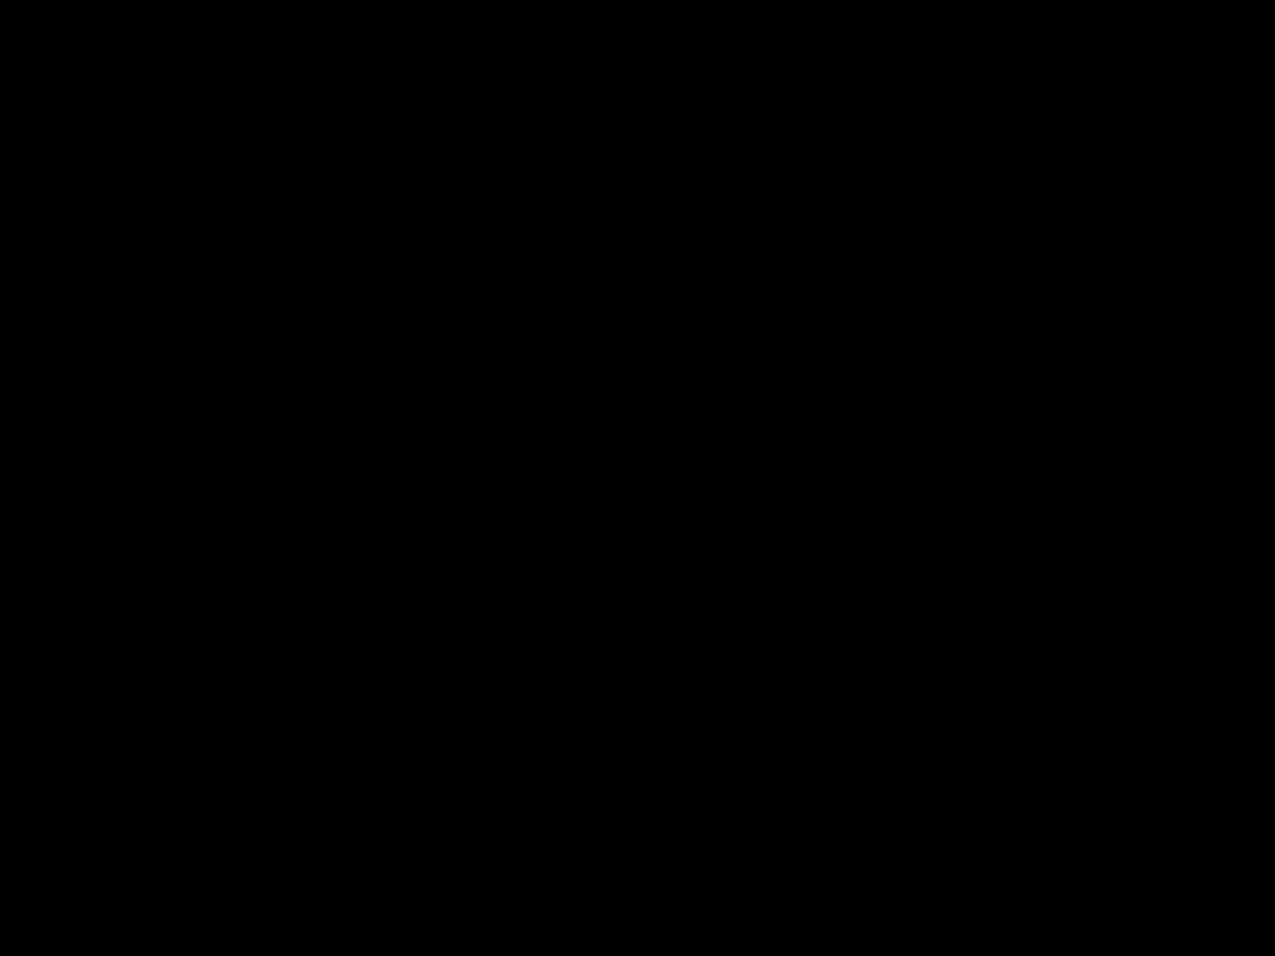
\includegraphics[width=110mm]{\FigDir/RED.pdf}
\caption{Reduction factor of the non infiltrating fraction as a function of rainfall.}
\label{fig:NonInfiltFrac}
\end{figure}
    
\subsubsection{Percolation}
If the soil moisture content of the root zone is above field capacity, water percolates to
the lower part of the potentially rootable zone and to the subsoil. In the model, a clear
distinction is made between percolation from the actual rootzone to the so-called lower
zone, and percolation from the lower zone to the subsoil. The former is called Perc and
the latter is called Loss. The percolation rate from the rooted zone can be calculated as:

\begin{equation}
\label{eq:6.21}
Perc  ~=~{\frac{W _{rz} \, -\, W _{rz,\, fc} }{\Delta t}} ~-~ T _{a} ~-~ E _{s} 
\end{equation}

Where:\\[5pt]
\begin{tabularx}{\textwidth}{llXr}
Perc &:& Percolation rate from the root zone to the lower zone  & [cm d$^{{\rm -1}}$]\\
W$_{{\rm rz}}$ &:& Amount of soil moisture in the root zone (see eq. \ref{eq:6.33}a)  & [cm]\\
W$_{{\rm rz,fc}}$ &:& Equilibrium amount of soil moisture in the root
   zone (see eq. \ref{eq:6.22})  & [cm]\\
$\Delta$t &:& Time step  & [d]\\
T$_{{\rm a}}$ &:& Actual transpiration rate (see eq. \ref{eq:6.14})  & [cm d$^{{\rm -1}}$]\\
E$_{{\rm s}}$ &:& Evaporation rate from a shaded soil surface 
  (see eq. \ref{eq:6.7}  and \ref{eq:6.20})  & [cm d$^{{\rm -1}}$]\\
\end{tabularx}

The equilibrium amount of soil moisture in the root zone can be calculated as the soil
moisture content at field capacity times the depth of the rooting zone:

\begin{equation}
\label{eq:6.22}
W _{rz,\, fc} ~=~ \theta  _{fc} \,\, RD
\end{equation}

Where:\\[5pt]
\begin{tabularx}{\textwidth}{llXr}
W$_{{\rm rz,fc}}$ &:& Equilibrium amount of soil moisture in the root zone  & [cm]\\
$\theta$$_{{\rm fc}}$ &:& Soil moisture content at field capacity  & 
    [cm$^{{\rm 3}}$ cm$^{{\rm -3}}$]\\
RD &:& Actual rooting depth  & [cm]\\
\end{tabularx}

The percolation rate is limited by the conductivity of the wet soil (acronym: {\bf SOPE}) in the
same way as the infiltration is limited. The conductivity is soil specific and should be
given by the user. Note that the percolation from the root zone to the lower zone can be
limited by the up take capacity of the lower zone. Therefore, the value calculated with 
equation \ref{eq:6.21} is preliminary. The capacity should first be checked.

The percolation from the lower zone to the subsoil, the so-called Loss, should take the
amount of water in the lower zone into account. If the amount of water in the lower zone
is less than the equilibrium amount of soil moisture, a part of the percolating water will
be retained and the percolation rate will be reduced. The loss of water from the lower end
of the maximum root zone can be calculated as:

\begin{equation}
\label{eq:6.23}
Loss ~=~{\frac{W _{lz} \, -\, W _{lz,\, fc} }{\Delta t}} ~+~ Perc
\end{equation}

Where:\\[5pt]
\begin{tabularx}{\textwidth}{llXr}
Loss &:& Percolation rate from the lower zone to the subsoil   & [cm d$^{{\rm -1}}$]\\
Perc &:& Percolation rate from root zone to lower zone (see eq. \ref{eq:6.21})  & [cm d$^{{\rm -1}}$]\\
W$_{{\rm lz}}$ &:& Amount of soil moisture in the lower zone (see eq. \ref{eq:6.33}b)  & [cm]\\
W$_{{\rm lz,fc}}$ &:& Equilibrium amount of soil moisture in the
   lower zone (see eq. \ref{eq:6.24})  & [cm]\\
$\Delta$t &:& Time step   & [d]\\
\end{tabularx}

The loss of water from the potentially rootable zone, is also limited by the maximum
percolation rate of the subsoil. This maximum percolation rate (acronym: {\bf KSUB}) is soil
specific and should be provided by the user. The equilibrium amount of soil moisture in
the lower zone can be calculated as the soil moisture content at field capacity times the
depth of the root zone:

\begin{equation}
\label{eq:6.24}
W_{lz,\, fc} = \theta_{fc} \,\, (RD_{\max} ~-~RD)
\end{equation}

Where:\\[5pt]
\begin{tabularx}{\textwidth}{llXr}
W$_{{\rm rz,fc}}$ &:& Equilibrium amount of soil moisture in the lower zone  & [cm]\\
$\theta$$_{{\rm fc}}$ &:& Soil moisture content at field capacity  & [cm$^{{\rm 3}}$ cm$^{{\rm -3}}$]\\
RD$_{{\rm max}}$ &:& Maximum rooting depth  & [cm]\\
RD &:& Actual rooting depth  & [cm]\\
\end{tabularx}

For rice an additional limit of five percent of the saturated soil conductivity is set to
account for the effect of puddling (a rather arbitrary value, which may be easily changed
in the program). The saturated soil conductivity (acronym: {\bf K0}) is soil specific. In the
model, K0 is calculated using equating \ref{eq:6.67} with pF= -1.0 (i.e. a hydraulic head of 0.1
cm) The percolation rate from the lower zone to the sub soil is not to exceed this value
(van Diepen {\it et al}., 1988). 

As mentioned before, the value calculated with equation \ref{eq:6.21}, should be regarded as
preliminary. The storage capacity of the receiving layer may become limiting. The
storage capacity of the lower zone, also called the uptake capacity, is the amount of air
plus the loss (van Diepen {\it et al}., 1988). The storage capacity can de defined as:

\begin{equation}
\label{eq:6.25}
UP  ~=~{\frac{(\, RD _{\max } \, -\, RD\, )\, \theta  _{\max } ~-~ W _{lz} }{\Delta t}} ~+~ Loss
\end{equation}

Where:\\[5pt]
\begin{tabularx}{\textwidth}{llXr}
UP &:& Uptake capacity of lower zone  & [cm d$^{{\rm -1}}$]\\
RD$_{{\rm max}}$ &:& Maximum rooting depth  & [cm]\\
RD &:& Actual rooting depth  & [cm]\\
W$_{{\rm lz}}$ &:& Amount of soil moisture in lower zone  & [cm]\\
$\theta$$_{{\rm max}}$ &:& Soil porosity (maximum soil moisture)  & [cm$^{{\rm 3}}$ cm$^{{\rm -3}}$]\\
$\Delta$t &:& Time step  & [d]\\
Loss &:& Percolation rate from the lower zone to the subsoil   & [cm d$^{{\rm -1}}$]\\
\end{tabularx}

The percolation to the lower part of the potentially rootable zone can not exceed the
uptake capacity of the lower zone. Therefore the percolation rate is equal to the minimum
of the calculated percolation rate (eq. \ref{eq:6.21}) and the uptake.

\subsubsection{Preliminary infiltration}
The infiltration rate depends on the amount of available water and the infiltration capacity
of the soil. If the actual surface storage is less then or equal to 0.1 cm, the preliminary
infiltration capacity is simply described as:

\begin{equation}
\label{eq:6.26}
IN_{p} =~ (\, 1\, -\, F _{I} \, C _{I} \, )\, P~+~ I _{e~} +~ SS _{\frac{t}{ \Delta t}} 
\end{equation}

Where:\\[5pt]
\begin{tabularx}{\textwidth}{llXr}
IN$_{{\rm p}}$ &:& Preliminary infiltration rate  & [cm d$^{{\rm -1}}$]\\
F$_{{\rm I}}$ &:& Maximum fraction of rain not infiltrating during time step t  & [-]\\
C$_{{\rm I}}$ &:& Reduction factor applied to F$_{{\rm I}}$ as a function of the 
   precipitation intensity  & [-]\\
P &:& Precipitation intensity  & [cm d$^{{\rm -1}}$]\\
I$_{{\rm e}}$ &:& Effective irrigation  & [cm d$^{{\rm -1}}$]\\
SS$_{{\rm t}}$ &:& Surface storage at time step t (see eq. \ref{eq:6.29})  & [cm]\\
$\Delta$t &:& Time step  & [d]\\
\end{tabularx}

The maximum fraction of rain not infiltrating during time step t, {\bf F$_{{\rm I}}$} 
(acronym: {\bf NOTINF})
can be either set to a fixed value or be made variable by multiplying F$_{{\rm I}}$ 
with a precipitation dependent reduction factor {\bf C$_{{\rm I}}$} (acronym: {\bf NINFTB}). 
If the fraction is variable, it means that it is maximum for high rainfall amounts, and 
that it will be reduced for low rainfall. The user should provide F$_{{\rm I}}$. 
Values of the C$_{{\rm I}}$ table are included in the model and
are assumed to be fixed. The infiltration rate calculated is preliminary, as the storage
capacity of the soil is not yet taken into account. 

If the actual surface storage is more than 0.1 cm, the available water which can 
potentially infiltrate, is equal to the amount of water, present on the surface, that is supplied via
rainfall and irrigation and depleted via evaporation from the water surface:

\begin{equation}
\label{eq:6.27}
IN_{p} ~=~P~+~I _{e} ~-~ E _{w~} +~ SS _{\frac{t}{\Delta t}} 
\end{equation}

Where:\\[5pt]
\begin{tabularx}{\textwidth}{llXr}
IN$_{{\rm p}}$ &:& Preliminary infiltration rate  & [cm d$^{{\rm -1}}$]\\
P &:& Precipitation intensity  & [cm d$^{{\rm -1}}$]\\
I$_{{\rm e}}$ &:& Effective irrigation  & [cm d$^{{\rm -1}}$]\\
E$_{{\rm w}}$ &:& Evaporation rate from a shaded water surface  & [cm d$^{{\rm -1}}$]\\
SS$_{{\rm t}}$ &:& Surface storage at time step t (see eq. 6.29)  & [cm]\\
$\Delta$t &:& Time step  & [d]\\
\end{tabularx}
 
However, the infiltration rate is hampered by the conductivity of the soil. The calculated
infiltration rate cannot exceed the conductivity of the soil, which is used as an infiltration
limit. The conductivity of the soil (acronym: {\bf SOPE}) is soil specific and should be given
by the user.

\subsubsection{Adjusted infiltration}
The total loss of water from the root zone can now be calculated as the sum of the
transpiration, the evaporation and the percolation. The sum of this loss and the available
pore space in the root zone define the maximum infiltration rate. The preliminary
infiltration rate cannot exceed this value. The maximum possible infiltration rate is given
by:

\begin{equation}
\label{eq:6.28}
IN_{\max } ~=~{\frac{(\, \theta  _{\max } \, -\, \theta  _{t} \, )\, RD}{\Delta t}} ~+~ T _{a} ~+~ E _{s} ~+~ Perc
\end{equation}

Where:\\[5pt]
\begin{tabularx}{\textwidth}{llXr}
IN$_{{\rm max}}$ &:& Maximum infiltration rate  & [cm d$^{{\rm -1}}$]\\
$\theta$$_{{\rm max}}$ &:& Soil porosity (maximum soil moisture)  
    & [cm$^{{\rm 3}}$ cm$^{{\rm -3}}$]\\
$\theta$$_{{\rm t}}$ &:& Actual soil moisture content  
    & [cm$^{{\rm 3}}$ cm$^{{\rm -3}}$]\\
RD &:& Actual rooting depth  & [cm]\\
$\Delta$t &:& Time step  & [d]\\
T$_{{\rm a}}$ &:& Actual transpiration rate   & [cm d$^{{\rm -1}}$]\\
E$_{{\rm s}}$ &:& Evaporation rate from a shaded soil surface  & [cm d$^{{\rm -1}}$]\\
Perc &:& Percolation rate from root zone to lower zone  & [cm d$^{{\rm -1}}$]\\
\end{tabularx}

\subsubsection{Surface runoff}

Surface runoff is also taken into account by defining a maximum value for the surface
storage. If the surface storage exceeds the maximum value for surface storage the
exceeding amount of water will run off. The surface storage at time step t can be
calculated as:

\begin{equation}
\label{eq:6.29}
SS_{t} ~=~ SS _{t-1} ~+~ (\, P ~+~ I _{e} ~-~ E _{w} ~-~ IN\, )\, \Delta t
\end{equation}

Where:\\[5pt]
\begin{tabularx}{\textwidth}{llXr}
SS$_{{\rm t}}$ &:& Surface storage at time step t  & [cm d$^{{\rm -1}}$]\\
P &:& Precipitation intensity  & [cm d$^{{\rm -1}}$]\\
I$_{{\rm e}}$ &:& Effective irrigation rate  & [cm d$^{{\rm -1}}$]\\
E$_{{\rm w}}$ &:& Evaporation rate from a shaded water surface  & [cm d$^{{\rm -1}}$]\\
IN &:& Infiltration rate (adjusted)  & [cm d$^{{\rm -1}}$]\\
\end{tabularx}

The surface runoff can be calculated as:

\begin{equation}
%6.30
SR_{t} = SS_{t} - \min (SS_{t}, SS_{\max})\\
\end{equation}

Where:\\[5pt]
\begin{tabularx}{\textwidth}{llXr}
SR$_{{\rm t}}$ &:& Surface runoff at time step t  & [cm]\\
SS$_{{\rm t}}$ &:& Surface storage at time step t  & [cm]\\
SS$_{{\rm max}}$ &:& Maximum surface storage  & [cm]\\
\end{tabularx}
 
{\bf SS$_{{\rm max}}$} (acronym: {\bf SSMAX}) is an environmental specific variable 
and should be provided by the user.

\subsubsection{Rates of change and root extension}
The rates of change in the amounts of water in the root zone and the lower zone are
calculated straightforward from the flows found above:

\stepcounter{equation}
\begin{align}
\label{eq:6.31}
\Delta W _{rz} &=~ (IN ~-~ T _{a} ~-~ E _{s} ~-~ Perc)\,\Delta \, t  \subeqn  \\
\Delta W _{lz} &=~ (Perc ~-~ Loss)\,\Delta \, t \subeqn
\end{align}

Where:\\[5pt]
\begin{tabularx}{\textwidth}{llXr}
$\Delta$W$_{{\rm rz}}$ &:& Change of the amount of soil moisture in the root zone  & [cm]\\
$\Delta$W$_{{\rm lz}}$ &:& Change of the amount of soil moisture in the lower zone  & [cm]\\
T$_{{\rm a}}$ &:& Actual transpiration rate   & [cm d$^{{\rm -1}}$]\\
E$_{{\rm s}}$ &:& Evaporation rate from a shaded soil surface  & [cm d$^{{\rm -1}}$]\\
IN &:& Infiltration rate  & [cm d$^{{\rm -1}}$]\\
Perc &:& Percolation rate from root zone to lower zone  & [cm d$^{{\rm -1}}$]\\
Loss &:& Percolation rate from lower zone to sub soil  & [cm d$^{{\rm -1}}$]\\
$\Delta$t &:& Time step  & [d]\\
\end{tabularx}

Due to extension of the roots into the lower zone, extra soil moisture becomes available.
The amount of the extra soil moisture in the new rootzone and the amount of water in the
reduced lower zone can be calculated as:

\begin{equation}
\label{eq:6.32}
\Delta W _{rz} ~=~\Delta W _{lz} ~=~ W _{lz} \,{\frac{ RD _{t} \, -\, RD _{t-1} }{RD _{\max } \, -\, RD _{t-1} }}
\end{equation}

Where:\\[5pt]
\begin{tabularx}{\textwidth}{llXr}
RD$_{{\rm t}}$ &:& Rooting depth at time step t  & [cm]\\
RD$_{{\rm t-1}}$ &:& Rooting depth at time step t-1  & [cm]\\
RD$_{{\rm max}}$ &:& Maximum rooting depth  & [cm]\\
W$_{{\rm lz}}$ &:& Amount of soil moisture in the lower zone (see eq. \ref{eq:6.33}b)  & [cm]\\
$\Delta$W$_{{\rm rz}}$ &:& Change of the amount of soil moisture in the root zone  & [cm]\\
$\Delta$W$_{{\rm lz}}$ &:& Change of the amount of soil moisture in the lower zone  & [cm]\\
\end{tabularx}

With equation \ref{eq:6.31} the actual amount of water in the root zone and in the lower zone can
be calculated according to:

\stepcounter{equation}
\begin{align}
\label{eq:6.33}
W _{rz,t} ~=~ W _{rz, t-1} ~+~ \Delta W _{rz} \subeqn  \\
W _{lz,t} ~=~ W _{lz, t-1} ~\, +~ \Delta W _{lz} \subeqn
\end{align}

Where:\\[5pt]
\begin{tabularx}{\textwidth}{llXr}
W$_{{\rm rz,t}}$ &:& Amount of soil moisture in the root zone at time step t  & [cm]\\
W$_{{\rm lz,t}}$ &:& Amount of soil moisture in the lower zone at time step t  & [cm]\\
W$_{{\rm rz,t-1}}$ &:& Amount of soil moisture in the root zone at time step t-1  & [cm]\\
W$_{{\rm lz,t-1}}$ &:& Amount of soil moisture in the lower zone at time step t-1  & [cm]\\
$\Delta$W$_{{\rm rz}}$ &:& Rate of change of the amount of soil moisture in the root 
   zone  & [cm]\\
$\Delta$W$_{{\rm lz}}$ &:& Rate of change of the amount of soil moisture in the 
   lower zone  & [cm]\\
\end{tabularx}

\subsubsection{Actual soil moisture content}
The actual soil moisture content can now be calculated according to (see also eq. \ref{eq:6.1}):

\begin{equation}
\label{eq:6.34}
\theta _{t} ~=~ W _{\frac{rz, t}{RD}} 
\end{equation}

Where:\\[5pt]
\begin{tabularx}{\textwidth}{llXr}
$\theta$$_{{\rm t}}$ &:& Actual soil moisture content at time step t  & [cm$^{{\rm 3}}$ cm$^{{\rm -3}}$]\\
W$_{{\rm rz,t}}$ &:& Amount of soil moisture in the root zone at time step t  & [cm]\\
RD &:& Actual rooting depth  & [cm]\\
\end{tabularx}


\section{System with groundwater influence  }
\label{sec:WATGW}

In the subroutine {\bf WATGW} the variables of the soil water balance in the actual 
water-limited production situation are calculated. Influence from groundwater is assumed. The
purpose is to quantify the crop water requirements for continuous growth with either
drought stress or water excess, and to quantify a possible reduction of the crop transpiration 
rate, leading to a reduced growth.

\subsection{Submodel with groundwater influence  }

The textural profile of the soil is conceived as homogeneous. Three soil zones are
distinguished in this system:\\

\begin{itemize}
 \item the rooted zone between soil surface and actual rooting depth;
 \item the zone between rooting depth and groundwater;
 \item the soil below groundwater level to a reference depth of 1000 centimeters. This
 reference depth is used to calculate a system water balance. It is a formal system
 boundary.
\end{itemize}
 
The extension of the root zone from initial rooting depth is described in \S \ref{sec:rootgrowth}. 
Its effect on the soil moisture content is accounted for in this soil water balance calculation.
From the moment that the maximum rooting depth is reached the soil profile is described
as a two layer system, because then the lower zone no longer exists.

Two situations are distinguished: with artificial drainage and without artificial drainage.
The soil water balance is calculated for a cropped field in the water-limited production
situation. The purpose of the calculations is to estimate the daily value of the mean soil
moisture content, because this variable influences uptake and crop transpiration and thus
the assimilation.

The water balance is driven by rainfall, possibly buffered as surface storage and
evapotranspiration. The processes considered are infiltration, soil water retention, the
steady state flow between the root zone and the groundwater table (capillary rise($\uparrow$) or
percolation($\downarrow$)), and drainage rate. An irrigation term is included but not used. The
resulting depth, moisture and air contents in the root zone are calculated. The calculation
of the evaporation rate, the preliminary infiltration rate, the precipitation as well as the
surface storage and runoff, in the system with groundwater influence, do not differ from
the processes in the system without groundwater influence. Therefore, for a description of
these processes one should see \S \ref{sec:evapotranspiration} and \S \ref{sec:WBElements}.

Groundwater influence is taken into account by calculation of capillary rise for a
stationary situation for a homogeneous soil. The time step of one day implies that
realization of some of the calculated flow rates over a whole day could result in moisture
contents exceeding the total pore space. This clearly sets limits to the values of these rates
of change. As a consequence, the model has more or less the character of a bookkeeping
system. The rate of capillary rise or percolation determine the change in groundwater
level. The new groundwater level is thus estimated from the calculated capillary rise or
percolation. The soil moisture profile in the soil between groundwater and rooted zone, is
assumed to be again in equilibrium. (in fact a contradiction with capillary rise or
percolation).

Difficulty arises when the groundwater rises into the rooted zone. The following procedure is 
then applied:
\begin{itemize}
\item To simplify the calculations, it is assumed that in the current time step the
  groundwater can rise at its highest level until the lower boundary of the rooted
  zone.
\item In the next time step the soil air content of the rooted zone is calculated. If the
  amount of water in the rooted zone increases, a subdivision is made between a
  lower, saturated, layer and the higher layer with the original air content and soil
  moisture content. The groundwater table is situated at the boundary between these
  zones. The root zone may be completely filled. Then the groundwater level is
  zero.
\item Loss of water from the rooted zone implies a rise of the groundwater level. In
  case so much water is lost, the groundwater level may drop below the rooted
  zone. The increase of soil moisture in the zone between groundwater and root
  zone is considered as capillary rise.
\end{itemize}
 
No capillary flow occurs if the groundwater table is within the root zone. The simulation
stops if the following circumstances arise:
\begin{itemize}
\item In case waterlogging occurs (i.e. groundwater depth less then 10 cm) and the
  plants cannot form airducts.
\item In case the plants can form airducts but waterlogging prevails for more then ten
  consecutive days.
\end{itemize}

\subsection{Root extension and the actual soil moisture content  }

The elements of the water balance have to be established before the actual soil moisture
content can be calculated. Therefore, in the following paragraph the percolation or
capillary rise, the adjusted infiltration and the actual soil moisture amount are treated
first. The calculation of the evaporation rate, the preliminary infiltration rate, the
precipitation as well as the surface storage and the surface runoff are not treated. These
processes are described earlier in \S \ref{sec:evapotranspiration} and \S \ref{sec:WBElements}. 
The new level of the groundwater
table is also established. The depth of the groundwater table is needed to calculate the
capillary rise (subroutine {\bf SUBSOL}). The effect of root extension will be explained at the
end of this paragraph.

\subsubsection{Initialization}
Some remarks have to be made on the initialization. The soil moisture content values at
field capacity, wilting point and the soil porosity are derived from the water retention
curve, $\theta$$_{{\rm log(}{\rm \Psi}{)}}$ (see eq. \ref{eq:6.38}). An AFGEN table (acronym: 
{\bf SMTAB}) with the $^{{\rm 10}}$log of the
matric head (pF) as the independent variable is used to describe this curve (see Appendix
2). The water retention curve is soil specific and should be provided by the user. The soil
moisture content at field capacity, {\bf $\theta$$_{{\rm fc}}$} (acronym: {\bf SMFCF}), 
the soil moisture content at
wilting point, {\bf $\theta$$_{{\rm wp}}$} (acronym: {\bf SMW}) and the soil porosity, 
{\bf $\theta$$_{{\rm max}}$} (acronym: {\bf SM0}) are
established using the AFGEN tale mentioned above with a matric head of 200 cm, 16000
cm and 0.1 cm respectively. In the model a pF table is constructed (acronym: {\bf PFTAB}).
It is the inverse of the SMTAB table.

First, the model calculates a table with values of the cumulative soil air volume above the
groundwater level at equilibrium. Under equilibrium conditions, the matric head values
are numerically equal to the height at which they occur. With soil air volume, the
cumulative amount of air as a function of height above groundwater under equilibrium
conditions is meant (acronym: {\bf SDEFTB}). The values of the cumulative amount of air for
the following values of height (matric head, also called soil suction): 0,2,4,8,16,32,64,
128,..,16384 cm are calculated and put into an AFGEN table. 

To calculate the cumulative air amount, the soil air content has to be integrated over the
intervals mentioned above. The three point Gaussian integration method is used in the
model. The length of the integration interval is given by:

\begin{equation}
\label{eq:6.35}
\Delta  \psi ~=~ \psi _{1} ~-~ \psi _{0} 
\end{equation}

Where:\\[5pt]
\begin{tabularx}{\textwidth}{llXr}
$\Delta$$\psi$ &:& Height of interval matric head  & [cm]\\
$\psi$$_{{\rm 0}}$ &:& Lower boundary interval matric head  & [cm]\\
$\psi$$_{{\rm 1}}$ &:& Upper boundary interval matric head  & [cm]\\
\end{tabularx}

Within each interval, three points are selected and used by the Gaussian integration, to
integrate over the interval are given by:

\begin{equation}
\label{eq:6.36}
 \Delta  \psi _{i} ~=~ (0.5 ~+~ p \sqrt{0.15} ) \Delta  \psi ~~~~~p~=~-1,0,1
\end{equation}

Where:\\[5pt]
\begin{tabularx}{\textwidth}{llXr}
$\psi$$_{{\rm i}}$ &:& Matric head   & [cm]\\
p &:& Three points for Gaussian integration  & [-]\\
\end{tabularx}

The average air content for the selected matric head can be calculated as:

\begin{equation}
\label{eq:6.37}
\theta  _{air, \psi _{i} } ~=~ \theta _{\max } ~-~ \theta  _{\psi _{i} }
\end{equation}

Where:\\[5pt]
\begin{tabularx}{\textwidth}{llXr}
$\theta$$_{{\rm air,}{\rm \Psi}{i}}$ &:& Air content at selected matric head  
    & [cm$^{{\rm 3}}$ cm$^{{\rm -3}}$]\\
$\theta$$_{{\rm max}}$ &:& Soil porosity  & [cm$^{{\rm 3}}$ cm$^{{\rm -3}}$]\\
$\theta$$_{{\rm \Psi}{i}}$ &:& Actual soil moisture content as a function of matric head  
    & [cm$^{{\rm 3}}$ cm$^{{\rm -3}}$]\\
\end{tabularx}

The actual soil moisture content can be derived as a function of the selected matric head
by using the soil specific water retention curve:

\begin{equation}
\label{eq:6.38}
\theta_{\psi_{i}} = \theta_{{\rm log} (\psi_{0} + \Delta \psi_{i})}
\end{equation}

Where:\\[5pt]
\begin{tabularx}{\textwidth}{llXr}
$\theta$$_{{\rm \Psi}{i}}$ &:& Actual soil moisture content as a function of 
    matric head  & [cm$^{{\rm 3}}$ cm$^{{\rm -3}}$]\\
$\Delta$$\psi$ &:& Height of interval matric head  & [cm]\\
$\psi$$_{{\rm 0}}$ &:& Lower boundary interval matric head  & [cm]\\
\end{tabularx}

Using the equations 6.35, 6.36, 6.37 and 6.38, the cumulative amount of air as a function
of height above groundwater under equilibrium conditions can now be calculated as: 

\begin{equation}
\label{eq:6.39}
A_{air} (h) ~=~\Delta  \psi \,{\frac{ \theta_{air, -1} ~+~ 1.6\, \theta_{air,0} ~+~ \theta_{air,1} }{3.6}}
\end{equation}

Where:\\[5pt]
\begin{tabularx}{\textwidth}{llXr}
A$_{{\rm air}}$(h) &:& Amount of air as a function of height (h) above
   groundwater table   & [cm]\\
$\Delta$$\psi$ &:& Height of interval matric head  & [cm]\\
$\theta$$_{{\rm air,p}}$ &:& Air content at selected matric head 
   p=-1,0,1  & [cm$^{{\rm 3}}$ cm$^{{\rm -3}}$]
\end{tabularx}

The AFGEN table, the matric head (or height above groundwater) as a function of the
cumulative air amount, $\psi$(A$_{{\rm air}}$) (acronym: {\bf DEFDTB}), is also calculated in the model. It is
the inverse of the table calculated above.

With the use of equation \ref{eq:6.39}, the soil air amount above the water table at equilibrium,
the initial state variables of the water balance can be computed. These are, the equilibrium 
amount of moisture in the subsoil, in the root zone and above the drains up to the
surface. Before this can be done however, the soil air volume below the rooted zone, in
the root zone and above the drains up to the surface has to be established. To estimate the
amount of air at a specific depth at equilibrium, the height of that specific level above soil
water table is used. It is assumed that in the rootzone no gradient exists. 

The equilibrium amount of moisture in the subsoil, the root zone and above the drains up
to the surface can than be calculated as:

\stepcounter{equation}
\begin{align}
\label{eq:6.40}
W_{ss,\, fc} &=~ (\, D_{\max} ~-~ RD\, )\, \theta_{\max } ~-~ A_{air} (h_{1} )
    \subeqn  \\
W_{rz,\, fc} &=~ RD\, \theta_{\max } ~+~A_{air} (h_{1} )~-~A_{air} (h_{2} ) 
   \subeqn  \\
W_{dd,\, fc} &=~ DD\, \theta_{\max } ~-~A _{air} (h_{3} )~~\, 
   \subeqn
\end{align}

Where:\\[5pt]
\begin{tabularx}{\textwidth}{llXr}
h$_{1}$ &:& Z$_{t~}$ - RD & [cm]\\
h$_{2}$ &:& Z$_{t}$  & [cm]\\
h$_{3}$ &:& DD  & [cm]\\

W$_{{\rm ss,fc}}$ &:& Equilibrium soil moisture amount below rooted zone  & [cm]\\
W$_{{\rm rz,fc}}$ &:& Equilibrium soil moisture amount in rooted zone  & [cm]\\
W$_{{\rm dd,fc}}$ &:& Equilibrium soil moisture amount above the drains up 
   to the surface  & [cm]\\
A$_{{\rm air}}$(h) &:& Amount of air as a function of height above groundwater
   table (see eq. \ref{eq:6.39})  & [cm]\\
$\theta$$_{{\rm max}}$ &:& Soil porosity  & [cm$^{{\rm 3}}$ cm$^{{\rm -3}}$]\\
RD &:& Actual rooting depth  & [cm]\\
DD &:& Drain depth  & [cm]\\
Z$_{{\rm t}}$ &:& Depth of groundwater table at time step t  & [cm]\\
\end{tabularx}

In the model, the initial moisture content in the rooted zone is assumed to be equal to the
equilibrium amount of moisture in the root zone if the groundwater level is within 100 cm
from the root zone or even in the root zone. If the groundwater level is lower than 100
cm below the root zone the initial moisture content in the rooted zone is calculated as the
soil moisture at field capacity. The variable days since last rain, D$_{{\rm slr}}$, which is used to
calculate the evaporation rate from a shaded soil (see eq. \ref{eq:6.20}), is set to unity. In case the
soil moisture is lower than pF 3.0, a value of five days is assumed.

\subsubsection{Capillary rise and percolation}
If the groundwater level is within the root zone, capillary rise and percolation are set to
zero and no capillary rise or percolation has to be calculated. 
If the groundwater level is below the root zone, capillary rise and percolation are
calculated. From the pF of the root zone, the height difference between the lower
boundary of the root zone and the groundwater depth, and the table of the hydraulic
conductivity, the capillary flow from groundwater to the root zone can be calculated. The
pF can be derived via interpolation from the soil specific water retention curve. Capillary
flow is calculated separately in the subroutine {\bf SUBSOL}. Because of its complex 
calculations this subroutine is discussed separately in \S \ref{sec:CapillaryFlow}. 

For sandy soils, a shallow groundwater depth and a shallow root zone, the capillary flow
may be so large that the system becomes unstable. Therefore, the calculated flow rate is
limited to the flow rate that would exist in a state of equilibrium with the groundwater
level. This maximum flow in a state of equilibrium with the ground- water level can be
calculated as:

\begin{equation}
% 6.41
CR_{\max} ~=~{\frac{W_{rz,\, fc} ~-~ W_{rz} }{\Delta t}}
\end{equation}

Where:\\[5pt]
\begin{tabularx}{\textwidth}{llXr}
CR$_{{\rm max}}$ &:& Maximum flow rate calculated at equilibrium  & [cm d$^{{\rm -1}}$]\\
W$_{{\rm rz,fc}}$ &:& Equilibrium amount of water in the rooted
   zone (see eq. 6.40b)  & [cm]\\
W$_{{\rm rz}}$ &:& Actual amount of water in the rooted zone (see eq. \ref{eq:6.55}) & [cm]\\
$\Delta$t &:& Time step  & [d]\\
\end{tabularx}

A positive flow rate is defined as capillary rise whereas a negative flow rate is considered
as percolation. For rice crops the percolation is limited to 5\% of the estimated soil
specific hydraulic conductivity, to account for the effect of puddling. This is a rather
arbitrary value.

\subsubsection{Drainage}
The drainage rate is calculated only if there is artificial drainage and if the ground- water
level is above the drainage depth. For other cases the drainage depth is set to zero.
The drainage rate depends on the amount of water that could drain, and on the capacity of
the drainage system.

The capacity of the drainage system is calculated first as (van Diepen {\it et al}., 1988):

\begin{equation}
\label{eq:6.42}
DR _{\max } ~=~ 0.2\, K0
\end{equation}

Where:\\[5pt]
\begin{tabularx}{\textwidth}{llXr}
DR$_{{\rm max}}$ &:& Maximum drainage rate, equal to the drainage capacity  & [cm d$^{{\rm -1}}$]\\
K0 &:& Hydraulic conductivity at saturation   & [cm d$^{{\rm -1}}$]\\
\end{tabularx}

The hydraulic conductivity at saturation, {\bf K0}  (acronym: {\bf K0}), is soil specific. In the
model, K0 is calculated using equating \ref{eq:6.67} with pF= -1.0 (i.e. a matric head of 0.1
cm). If the groundwater table is below the root zone the amount of water which can be
drained is the amount of water between the drains and the root zone minus the equilibrium 
amount which corresponding with the groundwater level at drainage depth. In the
model it is assumed that the drainage rate is always positive or zero (in case RD $>$ DD
and W$_{{\rm rz}}$ $<$ W$_{{\rm dd,fc}}$).

The drain depth, {\bf DD} (acronym: {\bf DD}) should be given be the user. The drainage rate can
be calculated as:

\begin{equation}
\label{eq:6.43}
DR ~=~{\frac{W _{rz} ~+~ (DD\, -\, RD)\, \theta _{\max } ~-~ W _{dd\, ,\, fc} }{\Delta t}}
\end{equation}

Where:\\[5pt]
\begin{tabularx}{\textwidth}{llXr}
DR &:& Drainage rate  & [cm d$^{{\rm -1}}$]\\
W$_{{\rm rz}}$ &:& Amount of water in the root zone (see eq. \ref{eq:6.55})  & [cm]\\
DD &:& Drain depth  & [cm]\\
RD &:& Actual rooting depth  & [cm]\\
$\theta$$_{{\rm max}}$ &:& Soil porosity  & [cm$^{{\rm 3}}$ cm$^{{\rm -3}}$]\\
W$_{{\rm dd,fc}}$ &:& Amount of water above drains (see eq. \ref{eq:6.40}c)  & [cm]\\
$\Delta$t &:& Time step  & [d]\\ 
\end{tabularx}

For groundwater located within the root zone the amount of water which can be drained
equals the water content of the root zone plus the water content of the (saturated) zone
between the drains and the rootzone, minus the equilibrium amount of water above the
drains. The drainage rate can be calculated as:

\begin{equation}
\label{eq:6.44}
DR = {\frac{A_{air} (h_{1}) - A_{air} (h_{2})}{\Delta t}}
\end{equation}

Where:\\[5pt]
\begin{tabularx}{\textwidth}{llXr}
DR &:& Drainage rate  & [cm d$^{{\rm -1}}$]\\
h$_{1}$ &:& DD - RD & [cm]\\
h$_{2}$ &:& Z$_{t~}$ - RD & [cm]\\
A$_{{\rm air}}$(h) &:& Amount of air as a function of height above groundwater
   table  (see eq. \ref{eq:6.39}) & [cm]\\
DD &:& Drain depth  & [cm]\\
RD &:& Actual rooting depth  & [cm]\\
Z$_{{\rm t}}$ &:& Depth of groundwater table at time step t  & [cm]\\
$\Delta$t &:& Time step  & [d]\\
\end{tabularx}

It should be noted that the drainage rate, calculated for both cases, cannot exceed the
drainage capacity of the system (eq. \ref{eq:6.42})

\subsubsection{Change of groundwater depth and adjustment of infiltration rate}

In the following text, the change of the groundwater and the adjustment of the infiltration
rate will be explained. Two different situations can be distinguished.
\begin{itemize}
\item Groundwater table below the rooted zone;
\item Groundwater table within the rooted zone.
\end{itemize}

In case the groundwater table is within the rooted zone, the water table might drop below
the rooted zone. In order to maintain a stable moisture content in the model, water is
recovered from the subsoil. In the water balance of the rooted zone this amount of water
is accounted for as capillary rise.

\subsubsection{Groundwater table below rootzone}
Now the change in the groundwater depth and the infiltration rate can be adjusted. If the
groundwater level is below the root zone the calculation is simple. From the drainage
rate, the rate of capillary rise and/or percolation rate, the new air amount between root
zone and groundwater can be found:

\begin{equation}
\label{eq:6.45}
 A_{new} ~=~ A_{air} (h) ~+~ (\, DR ~+~ CR ~-~ Perc\, )\, \Delta t
\end{equation}

Where:\\[5pt]
\begin{tabularx}{\textwidth}{llXr}
h &:& Z$_{t~}$ - RD & [cm]\\
A$_{{\rm new}}$ &:& New air amount between root zone and groundwater level  & [cm]\\
A$_{{\rm air}}$(h) &:& Amount of air as a function of height above groundwater
   table  (see eq. 6.39) & [cm]\\
RD &:& Actual rooting depth  & [cm]\\
Z$_{{\rm t}}$ &:& Depth of groundwater table at time step t  & [cm]\\
DR &:& Drainage rate  & [cm d$^{{\rm -1}}$]\\
CR &:& Rate of capillary rise (see \S \ref{sec:CapillaryFlow})  & [cm d$^{{\rm -1}}$]\\
Perc &:& Percolation rate  & [cm d$^{{\rm -1}}$]\\
\end{tabularx}

To simplify calculations, the groundwater is not allowed to enter the root zone in the
current time step. This could happen in case the new air amount between ground-water
and root zone, A$_{{\rm new}}$, assumes a negative value. The groundwater level is allowed to rise
maximally till the lower boundary of the root zone (A$_{{\rm new}}$=0). In the next time step the
groundwater may rise further. Therefore, the percolation rate is constrained to prevent
such an occasion. 

\begin{equation}
\label{eq:6.46}
Perc ~=~Perc ~+~{\frac{A _{new} }{\Delta t}}
\end{equation}

Where:\\[5pt]
\begin{tabularx}{\textwidth}{llXr}
Perc &:& Percolation rate   & [cm d$^{{\rm -1}}$]\\
A$_{{\rm new}}$ &:& New air amount between root zone and groundwater table  & [cm]\\
$\Delta$t &:& Time step  & [d]\\
\end{tabularx}

The definitive value of the percolation is now known and used to constrain the rate of the
maximum possible infiltration rate. This is done in order to prevent an over saturated root
zone.

The maximum possible infiltration equals the available soil air volume which is given by:

\begin{equation}
\label{eq:6.47}
IN_{\max } ~=~{\frac{(\, \theta _{\max } ~-~ \theta _{t} ~-~ 0.0004\, )\, RD}{\Delta t}} ~+~ T _{a} ~+~ E _{s} ~+~ Perc ~-~ CR
\end{equation}

Where:\\[5pt]
\begin{tabularx}{\textwidth}{llXr}
IN$_{{\rm max}}$ &:& Maximum infiltration rate  & [cm d$^{{\rm -1}}$]\\
$\theta$$_{{\rm max}}$ &:& Soil porosity  & [cm$^{{\rm 3}}$ cm$^{{\rm -3}}$]\\
$\theta$$_{{\rm t}}$ &:& Soil moisture content (see eq. \ref{eq:6.56})  
    & [cm$^{{\rm 3}}$ cm$^{{\rm -3}}$]\\
RD &:& Actual rooting depth  & [cm]\\
$\Delta$t &:& Time step  & [d]\\
T$_{{\rm a}}$ &:& Actual transpiration  & [cm d$^{{\rm -1}}$]\\
E$_{{\rm s}}$ &:& Evaporation rate of shaded soil surface  & [cm d$^{{\rm -1}}$]\\
Perc &:& Percolation rate  & [cm d$^{{\rm -1}}$]\\
CR &:& Rate of capillary rise  & [cm d$^{{\rm -1}}$]\\
\end{tabularx}

The soil moisture content of the root zone is limited to a value just below saturation to
prevent zero air content in the root zone, which could lead to problems in the next time
step if, at that day, the groundwater enters the rooted zone. The adjusted infiltration rate
(see eq. \ref{eq:6.26} and \ref{eq:6.27}) is established by limiting the preliminary infiltration to maximum
possible infiltration rate.

The equilibrium profile is assumed and the new height of the root zone above the
groundwater level (i.e. matric head at the root tip) can now be obtained from the relation
between height above the groundwater table and the cumulative air amount $\psi$(A$_{{\rm air}}$), by
introducing the new air amount between the root zone and the groundwater level, A$_{{\rm new}}$,
into this relation. Adding the actual rooting depth, RD, yields the depth of the groundwater 
table. The rate of change of the groundwater level is found by subtracting the old
value of the groundwater depth from the new value of the groundwater depth. 

\begin{equation}
\label{eq:6.48}
\Delta Z = {\frac{\psi (A_{new} ) + RD - Z_{t-1}}{\Delta t}}
\end{equation}

Where:\\[5pt]
\begin{tabularx}{\textwidth}{llXr}
$\Delta Z$ &:& Change in groundwater level per time step  & [cm d$^{ -1}$]\\
$\psi$() &:& Matric head as a function of the amount of air  & [cm]\\
$A_{new}$ &:& New air amount between root zone and groundwater
   level (see eq. \ref{eq:6.45})  & [cm]\\
$RD$ &:& Actual rooting depth  & [cm]\\
$Z_{t-1}$ &:& Depth of groundwater table at time step t-1  & [cm]
\end{tabularx}

The initial depth of the groundwater table (acronym: {\bf ZTI}) should be provided by the
user. 

\subsubsection{Groundwater table within the rooted zone}
When the groundwater enters the rooted zone, the air concentration in the root zone is
calculated. The percolation is assumed to equal the maximum drainage rate. The root
zone is divided into a part saturated with water, and an unsaturated part. The initial air
concentration is maintained in the unsaturated part. This implies that an increase of the
water content leads to a shallower unsaturated part and hence to a rising groundwater
level.

This rather artificial construction is necessary because of the inter-dependence of the
water content and the groundwater depth. In this system the relation between water
content and groundwater depth is (van Diepen {\it et al}., 1988):

\begin{equation}
\label{eq:6.49}
Z_{t} \cdot \theta_{air,t} = RD \cdot \theta_{max} - W_{t} 
\end{equation}

Where:\\[5pt]
\begin{tabularx}{\textwidth}{llXr}
$Z_{t}$ &:& Depth of groundwater table at time step t  & [cm]\\
$\theta$$_{{\rm air,t}}$ &:& Air content above groundwater table  
    & [cm$^{{\rm 3}}$ cm$^{{\rm -3}}$]\\
$RD$ &:& Actual rooting depth  & [cm]\\
$\theta_{ma}$ &:& Soil porosity  & [cm$^{{\rm 3}}$ cm$^{{\rm -3}}$]\\
$W_{ t}$ &:& Amount of water in the root zone (see eq. \ref{eq:6.55})  & [cm]\\
\end{tabularx}

Both sides of the expression equal the amount of air in the root zone. Note that on the
day at which the groundwater enters the root zone, the air content above the groundwater
table should assume a non-zero value. This implies that the groundwater may not rise
from below the root zone to the soil surface in one time step. Moreover, at the day at
which the groundwater enters the root zone, the soil should not be saturated. This is in
fact the same condition as the first one. 

When the groundwater is within the root zone, the drainage rate is equivalent to the rate
of percolation. The preliminary infiltration rate (see e.q. \ref{eq:6.26} and \ref{eq:6.27}) 
cannot exceed
the available soil air volume ('over saturation'). The adjusted infiltration rate is thus
established by limiting the preliminary infiltration to the available soil air volume. The
maximum value the adjusted infiltration rate can reach is defined as:

\begin{equation}
\label{eq:6.50}
IN_{max} = {\frac{\theta_{air,t} \cdot Z _{t}}{\Delta t}} + T_{a} + E_{s} + Perc
\end{equation}

Where:\\[5pt]
\begin{tabularx}{\textwidth}{llXr}
$IN_{max}$ &:& Maximum infiltration rate  & [cm d$^{{\rm -1}}$]\\
$Z_{t}$ &:& Depth of groundwater table at time step t  & [cm]\\
$\theta_{air,t}$ &:& Air content above groundwater table (see eq. \ref{eq:6.49})  
    & [cm$^{{\rm 3}}$ cm$^{{\rm -3}}$]\\
$T_{a}$ &:& Actual transpiration rate (see eq. 6.14)  & [cm d$^{-1}$]\\
$E_{s}$ &:& Evaporation rate of a shaded soil surface (see eq. \ref{eq:6.20})  
    & [cm d$^{{\rm -1}}$]\\
$Perc$ &:& Percolation rate  & [cm d$^{{\rm -1}}$]\\
\end{tabularx}

In the model, two different situations are distinguished. During the current time step the
groundwater stays within the root zone or the groundwater level drops below the root
zone. When the groundwater table stays within the root zone, the change in the depth of
the groundwater table can be established by using the rates of transpiration, evaporation,
percolation and infiltration. Transpiration, evaporation and percolation cause an increase
of the amount of air in the root zone, whereas the infiltration causes a decrease in the
amount of air. From these rates the change in groundwater depth follows. 

\begin{equation}
\label{eq:6.51}
\Delta Z ~=~{\frac{T _{a} ~+~ E _{s} ~+~ Perc ~-~ IN }{\theta _{air\, ,\, t} }}
\end{equation}

Where:\\[5pt]
\begin{tabularx}{\textwidth}{llXr}
$\Delta$Z &:& Change in groundwater level per time step  & [cm d$^{{\rm -1}}$]\\
IN &:& Infiltration rate  & [cm d$^{{\rm -1}}$]\\
T$_{{\rm a}}$ &:& Actual transpiration  & [cm d$^{{\rm -1}}$]\\
E$_{{\rm s}}$ &:& Evaporation rate  & [cm d$^{{\rm -1}}$]\\
Perc &:& Percolation rate  & [cm d$^{{\rm -1}}$]\\
$\theta$$_{{\rm air,t}}$ &:& Air content above groundwater table  & [cm$^{{\rm 3}}$ cm$^{{\rm -3}}$]
\end{tabularx}

When the groundwater level falls below the root zone, in order to maintain a stable
moisture content during the transition in the rooted zone, water is recovered from the
subsoil. In the water balance of the rooted zone this amount of water is accounted for as
capillary rise. (This rather artificial construction is used because the time step of one day
is too large to keep track of fluctuations of the groundwater level.)

\begin{equation}
\label{eq:6.52}
CR = {\frac{ (\Delta Z \cdot \Delta t - (RD - Z_{t})) \cdot \theta_{air, t} }{\Delta t}}
\end{equation}

Where:\\[5pt]
\begin{tabularx}{\textwidth}{llXr}
$CR$ &:& Rate of capillary rise  & [cm d$^{{\rm -1}}$]\\
$\Delta Z$ &:& Change in groundwater level per time step  & [cm d$^{-1}$]\\ 
$Z_{t}$ &:& Depth of groundwater table at time step  & [cm d$^{-1}$]\\
$\Delta t$ &:& Time step  & [d]\\
$RD$ &:& Actual rooting depth  & [cm]\\
$\theta_{air,t}$ &:& Air content above groundwater table  & [cm$^{{\rm 3}}$ cm$^{{\rm -3}}$]\\
\end{tabularx}

The equilibrium profile is assumed again. The new height of the root zone above the
groundwater level can now be obtained from the relation between height above the
groundwater table and the cumulative air amount $\psi$(A $_{{\rm air}}$), by introducing CR.$\Delta$t, 
the replaced air amount between the root zone and the groundwater level, into this relation.
and the rate of change of the groundwater depth can be found by subtracting the old value
of the groundwater depth from the new value of the groundwater depth (see eq. \ref{eq:6.48}). 

\subsubsection{Moisture amount}
The rate of change in amount of moisture in the root zone is calculated in a straightforward 
way from the calculated flow rates:

\begin{equation}
\label{eq:6.53}
\Delta W ~=~ -\, T _{a} ~-~ E _{s} ~-~ Perc ~+~ CR ~+~ IN
\end{equation}

Where:\\[5pt]
\begin{tabularx}{\textwidth}{llXr}
$\Delta$W &:& Rate of change in the amount of moisture in the root zone  & [cm d$^{{\rm -1}}$]\\
T$_{{\rm a}}$ &:& Actual transpiration rate  & [cm d$^{{\rm -1}}$]\\
E$_{{\rm s}}$ &:& Evaporation rate  & [cm d$^{{\rm -1}}$]\\
Perc &:& Percolation rate  & [cm d$^{{\rm -1}}$]\\
CR &:& Rate of capillary rise  & [cm d$^{{\rm -1}}$]\\
IN &:& Infiltration rate  & [cm d$^{{\rm -1}}$]\\
\end{tabularx}

\subsubsection{Root extension}
Due to extension of the roots into the lower zone, extra soil moisture becomes available.
The extra soil moisture added to the rooted zone by root growth can be calculated as:

\begin{equation}
\label{eq:6.54}
\Delta W_{rz} ~=~(RD _{t} \, -\, RD _{t-1} )~\theta _{\max } ~-~({\rm A} _{air} (h _{1} )~-~A _{air} (h _{2} ))  
\end{equation}

Where:\\[5pt]
\begin{tabularx}{\textwidth}{llXr}
h$_{1}$ &:& Z$_{t~}$ - RD$_{t~}$ & [cm]\\
h$_{2}$ &:& Z$_{t-1}$ - RD$_{t-1}$ & [cm]\\
$\Delta$W$_{{\rm rz}}$ &:& Change of the amount of soil moisture in the root zone  & [cm]\\
RD$_{{\rm t}}$ &:& Rooting depth at time step t  & [cm]\\
A$_{{\rm air}}$(h) &:& Amount of air as a function of height above groundwater 
   table  (see eq. \ref{eq:6.39}) & [cm]\\
Z$_{{\rm t}}$ &:& Depth of the groundwater table at time step t  & [cm]\\
$\theta_{{\rm max}}$ &:& Soil porosity  & [cm$^{{\rm 3}}$ cm$^{{\rm -3}}$]\\
\end{tabularx}

It is clear that the amount of air in the lower zone as well as the equilibrium soil moisture
amount below the rooted zone are reduced by the extension of the roots. With equation
\ref{eq:6.54} the actual amount of water in the root zone and in the lower zone can be calculated
according to:

\begin{equation}
\label{eq:6.55}
W_{rz,t} ~=~ W_{rz, t-1} ~+~ \Delta W_{rz} 
\end{equation}

Where:\\[5pt]
\begin{tabularx}{\textwidth}{llXr}
W$_{{\rm rz,t}}$ &:& Amount of soil moisture in the root zone at time step t  & [cm]\\
W$_{{\rm rz,t-1}}$ &:& Amount of soil moisture in the root zone at time step t-1  & [cm]\\
$\Delta$W$_{{\rm rz}}$ &:& Change of the amount of soil moisture in the root zone  & [cm]\\
\end{tabularx}

\subsubsection{Actual soil moisture content}
The actual moisture content can now be calculated according to (see also eq. 
\ref{eq:6.1} and \ref{eq:6.34}):

\begin{equation}
\label{eq:6.56}
\theta_{t} ~=~ W _{\frac{rz, t}{RD}} 
\end{equation}

Where:\\[5pt]
\begin{tabularx}{\textwidth}{llXr}
$\theta$$_{{\rm t}}$ &:& Actual soil moisture content at time step t  
    & [cm$^{{\rm 3}}$ cm$^{{\rm -3}}$]\\
W$_{{\rm rz,t}}$ &:& Amount of soil moisture in the root zone at time step t  & [cm]\\
RD &:& Actual rooting depth  & [cm]\\
\end{tabularx}

It should be mentioned that the simulation will be stopped in case more than ten successive
days of water logging occur and the crop cannot develop airducts. Water logging is defined
in the model as a groundwater depth of less than 10 cm.

\section{Calculation of capillary flow  }
\label{sec:CapillaryFlow}

In subroutine {\bf SUBSOL} the capillary flow is calculated. The capillary rise is defined as
the flow between the groundwater table and the root zone, whereas  percolation is defined
as the flow from the root zone to the groundwater. The flow is calculated for a stationary
situation, which means that the soil moisture profile does not change within one time step
of integration. The basic equation is given by:

\begin{equation}
\label{eq:6.57}
FL _{p} =~({\frac{d \psi }{ d\,\, Z _{rd} }} ~-~ 1)~K
\end{equation}

Where:\\[5pt]
\begin{tabularx}{\textwidth}{llXr}
FL$_{{\rm p}}$ &:& Flow rate  & [cm d$^{{\rm -1}}$]\\
Z$_{{\rm rd}}$ &:& Distance between root zone and groundwater table  & [cm]\\
K &:& Hydraulic conductivity  & [cm d$^{{\rm -1}}$]\\
$\psi$ &:& Matric head  & [cm]\\
\end{tabularx}

Equation \ref{eq:6.57} can be rewritten according to:

\begin{equation}
\label{eq:6.58}
d\, Z _{rd} ~=~{\frac{K\,\, d \psi }{ K ~+~ FL _{p} }}
\end{equation}

Where:\\[5pt]
\begin{tabularx}{\textwidth}{llXr}
Z$_{{\rm rd}}$ &:& Distance between root zone and groundwater table  & [cm]\\
K &:& Hydraulic conductivity  & [cm d$^{{\rm -1}}$]\\
$\psi$ &:& Matric head  & [cm]\\
FL$_{{\rm p}}$ &:& Flow rate  & [cm d$^{{\rm -1}}$]\\
\end{tabularx}

Between groundwater and rootzone a $\psi$-profile exists. An increase in Z implies an
increase in $\Psi$. Close to the groundwater, the hydraulic conductivity is relatively large and
the ratio K/(K+FL$_{{\rm p}}$) is close to unity. At some height above the groundwater table, the
hydraulic conductivity becomes smaller and the ratio starts to decrease fast. So, for a
large value of $\Psi$, a small increase of groundwater level will lead to large in $\Psi$\\
A stationary soil moisture profile implies a flow rate independent of the height above the
groundwater table. The hydraulic conductivity as a function of the $\Psi$ is known, so the
right hand side of equation \ref{eq:6.58} depends only on $\Psi$ and can be numerically integrated
over the interval (0-$\Psi$$_{{\rm rootzone}}$), at least, after an estimate of the flow has been made. If the
resulting height difference, Z$_{{\rm rd}}$, is equal to the real distance between rootzone and
groundwater, D, the estimated flow is correct. If Z$_{{\rm rd}}$ is greater than D, however, the
estimated flow is too low and if Z$_{{\rm rd}}$ is less than D, the estimated flow is too high. Via an
iteration procedure the value of flow can be adjusted until a satisfactory value is found.

\subsection{Initialization}
The matric head can be calculated from a pF curve using the following equation:

\begin{equation}
\label{eq:6.59}
\psi ~=~e ^{pF \cdot \ln(10)} 
\end{equation}

Where:\\[5pt]
\begin{tabularx}{\textwidth}{llXr}
$\psi$ &:& Matric head  & [cm]\\
pF &:& pF value  & [-]\\
\end{tabularx}

The pF value in equation \ref{eq:6.59} is calculated using the AFGEN table PFTAB with the soil
moisture content as the independent variable. The PFTAB table is constructed out of the
SMTAB table. If the calculated matric head is smaller than or equal to zero the hydraulic
conductivity is set equal to the saturated conductivity. For these conditions the flow can
be calculated as:

\begin{equation}
\label{eq:6.60}
FL~=~K\,{\frac{\psi }{D}} ~-~ 1
\end{equation}

Where:\\[5pt]
\begin{tabularx}{\textwidth}{llXr}
FL &:& Flow rate  & [cm d$^{{\rm -1}}$]\\
K  &:& Hydraulic conductivity  & [cm d$^{{\rm -1}}$]\\
$\Psi$ &:& Matric head  & [cm]\\
D &:& Height difference between the root zone and the groundwater table  & [cm]\\
\end{tabularx}

\subsection{Integration}
If the calculated matric head is positive, the flow rate has to be derived by means of an
iteration loop. However, first the number and width of the integration intervals has to be
established. The maximum number of integration intervals equals four, their width's are
defined as: [0-45 cm], [45-170 cm], [170-330 cm] and [330,$\Psi$$_{{\rm rootzone}}$].
To integrate the last interval, a logarithmic transformation is applied. This interval is then
written as ($^{{\rm 10}}$log(330), $^{{\rm 10}}$log($\Psi$$_{{\rm rootzone}}$)).
If for example the matric head is 220 cm, only three integration intervals will be
included: [0-45 cm], [45-170 cm], [170-220 cm]. If the matric head is larger than 330 cm
a fourth integration interval will be included. The width of the fourth interval will than be
calculated as pF minus $^{{\rm 10}}$log330. Using a logarithmic transformation, equation 
\ref{eq:6.55} becomes:

\begin{equation}
\label{eq:6.61}
dZ_{rd} = d pF{\frac{\ln(10) K 10^{pF} }{K + FL_{p}}}
\end{equation}

Where:\\[5pt]
\begin{tabularx}{\textwidth}{llXr}
Z$_{{\rm rd}}$ &:& Distance between root zone and groundwater table  & [cm]\\
K &:& Hydraulic conductivity  & [cm d$^{{\rm -1}}$]\\
pF &:& pF value  & [-]\\
FL$_{{\rm p}}$ &:& Flow rate  & [cm d$^{{\rm -1}}$]\\
\end{tabularx}

The three point Gaussian integration is used for the integration of $\Psi$ over the intervals
mentioned above. The length of each integration interval can be expressed as:

\begin{equation}
\label{eq:6.62}
\Delta \psi ~=~ \psi _{1} ~-~ \psi _{0} 
\end{equation}

Where:\\[5pt]
\begin{tabularx}{\textwidth}{llXr}
$\Delta$$\psi$ &:& Length of the interval matric head  & [cm]\\
$\psi$$_{{\rm 0}}$ &:& Lower boundary interval matric head  & [cm]\\
$\psi$$_{{\rm 1}}$ &:& Upper boundary interval matric head  & [cm]\\
\end{tabularx}

According to Gaussian integration method, three distances within the length of the
integration interval are selected. These distances are:

\begin{equation}
\label{eq:6.63}
\Delta \psi_{i} = (0.5 + p \sqrt{0.15}) \Delta \psi ~~~~ for ~~~~ p = -1, 0, 1 
\end{equation}

Where:\\[5pt]
\begin{tabularx}{\textwidth}{llXr}
$\Psi$$_{{\rm i}}$ &:& Matric head  & [cm]\\
p &:& Three points of the Gaussian integration\\
\end{tabularx}

The selected matric head values for Gaussian integration for each integration interval can
be calculated as:

\begin{equation}
\label{eq:6.64}
\psi ~=~ \psi _{0} ~+~\Delta \psi _{i} 
\end{equation}

Where:\\[5pt]
\begin{tabularx}{\textwidth}{llXr}
$\psi$ &:& Total selected matric head  & [cm]\\
$\psi$$_{{\rm 0}}$ &:& Lower boundary interval matric head  & [cm]\\
$\Delta$$\psi$$_{{\rm i}}$ &:& Selected matric head  & [cm]\\
\end{tabularx}

The selected matric head values can be expressed as pF-values according:

\begin{equation}
\label{eq:6.65}
pF ~=~\ ^{10} {\rm log} (\psi )
\end{equation}

Where:\\[5pt]
\begin{tabularx}{\textwidth}{llXr}
pF &:& pF-value  & [-]\\
$\psi$ &:& Matric head  & [cm]\\
\end{tabularx}

For the full-width integration intervals, the selected matric head values and therefore the
selected pF-values will always be the same. With the equations \ref{eq:6.62},  
\ref{eq:6.63} and \ref{eq:6.64}, the
three selected matric heads per interval for the Gaussian integration can be calculated.
With the help of equation \ref{eq:6.65}, the pF-values for the full-width integration intervals can
be calculated. The results are presented in Table \ref{tab:Table6.3}.

\begin{table}
%Table 6.3
\centering
\caption{pF values of the selected matric heads per interval}
\label{tab:Table6.3}
\begin{tabular}{l|rrr}
\hline
Interval & \multicolumn{3}{c}{pF values}\\
\hline
0, 45    & 0.705143  &  1.352183 &    1.601282    \\
45, 170  &  1.771497 &  2.031409 &    2.192880    \\
170, 330 &  2.274233 &  2.397940 &    2.494110    \\
\hline
\end{tabular}
\end{table}

The pF-values for the full width integration intervals are included in the subroutine
{\bf SUBSOL} in order to diminish calculation time. For different integration intervals the
calculations are the same. 

For the last interval, as mentioned before, a logarithmic transformation is applied. Instead
of matric head values, now three pF values are selected, using the Gaussian integration
method.

\begin{equation}
\label{eq:6.66}
\Delta pF_{i} = (0.5 + p \cdot \sqrt{0.15})\Delta pF ~~~~ for ~~~~ p = -1, 0, 1
\end{equation}

Where:\\[5pt]
\begin{tabularx}{\textwidth}{llXr}
pF$_{{\rm i}}$ &:& pF value  & [-]\\
p &:& Three points of the Gaussian integration\\
\end{tabularx}

As mentioned earlier, first the intervals have to be selected. For these intervals, for every
selected hydraulic head or pF-value (three per interval), the hydraulic conductivity is
computed using the following equation:

\begin{equation}
\label{eq:6.67}
K = e^{\ln(10) \cdot K(pF)} 
\end{equation}

Where:\\[5pt]
\begin{tabularx}{\textwidth}{llXr}
K &:& Hydraulic conductivity  & [cm d$^{{\rm -1}}$]\\
K(pF) &:& $^{{\rm 10}}$log of hydraulic conductivity as a function of pF  & [-]\\
\end{tabularx}

The $^{{\rm 10}}$log of hydraulic conductivity as a function of pF, {\bf K(pF)} 
(acronym: {\bf CONTAB}), is soil specific and should be provided by the user.
The values of K, calculated with equation \ref{eq:6.67}, are needed in the iteration loop to
calculate (K+FL$_{{\rm p}}$), the denominator of equation \ref{eq:6.58}. In the model, the nominator of the
right-hand side of equation \ref{eq:6.58} is integrated using the Gaussian integration. Therefore,
the K values are multiplied by the size of the interval ($\Delta$$\Psi$) and by the weighing factor
(see Appendix 1). The results are put in a help array.

\subsection{Iteration}
In order to find the correct flow rate in the iteration process, an upper limit and a lower
limit have to be established. The actual flow rate lies somewhere in between. The upper
limit of the flow rate is set to 1.27 cm d$^{{\rm -1}}$ and lower limit for the flow rate can be set as:

\begin{equation}
\label{eq:6.68}
FL_{l} = - e^{\ln(10) \cdot K(pF)}
\end{equation}

Where:\\[5pt]
\begin{tabularx}{\textwidth}{llXr}
FL$_{{\rm l}}$ &:& Lower limit for the flow rate  & [cm d$^{{\rm -1}}$]\\
K(pF) &:& Hydraulic conductivity as a function of the pF  & [-]\\
\end{tabularx}

The estimate of the flow rate is chosen halfway between the upper and lower limit. After
an estimate of the flow rate is made, the iteration process starts. The calculated height
above the groundwater table is compared with the real distance between root zone and
groundwater. Depending on the outcome, either the upper limit or the lower limit is
adjusted, and the process starts again. If the absolute error is smaller then 0.01 and the
relative error smaller than 0.1, the iteration is terminated. The iteration is limited to a
maximum of 15 steps.

It is assumed that the rate of capillary rise is never higher than 1.27 cm d$^{{\rm -1}}$. If 
the matric
head is smaller than the depth of the groundwater level, the upper limit for the flow rate
is set to zero. If the matric head is larger than the groundwater depth the lower limit is
set to zero. If the matric head is equal to the depth of the groundwater both, upper and
lower limit are set to zero and therefore the flow rate equals zero.


\backmatter
\appendix
\chapter*{APPENDIX 1}

\section*{Gaussian Integration}

The Gaussian integration method as applied in the model, is based on a study by Goudriaan
(1986). In the following text this method will be briefly explained.

The rate of crop photosynthesis can be computed from the photosynthesis - light response
curve of individual leaves, the incoming radiation and the leaf area index. Leaf area
distribution, extinction and reflection coefficients must also be known since they influence
the distribution of the available radiation. This computational problem was essentially solved
by De Wit (1965). He applied a stratification of the leaf canopy, calculated the absorbed
radiation and the corresponding rates of photosynthesis of sunlit and shaded leaves in each
layer. The contributions of the individual layers  were added to find the rate of crop
photosynthesis. This procedure was repeated every 15 minutes to obtain the daily total of
crop photosynthesis. This procedure is lucid and flexible, but rather time consuming.
Therefore, its use during an entire season as one would want in simulation of crop growth,
might become problematic.

For application in such models Goudriaan and Van Laar (1978) developed a summary model
for the daily total of crop photosynthesis, based on a semi-empirical equation, fitted to
computer output of the detailed model.

Usually integration in time or in spatial dimension is done by means of the well-known
numerical methods such as Eulerian (rectangular), Simpson or Runga - Kuta methods. These
methods are excellent and generally applicable because they permit feedback of the
integrated value (state variable) on the rate itself. But when there is no such feedback, and
the profile of the rate is known on forehand, a method, devised by the German
mathematician Gauss, is much more efficient and accurate. 

Several examples of processes where this feedback is absent can be defined in the crop
growth modeling. In those cases the Gaussian integration can be applied. Examples in the
WOFOST model where this method is used:
\begin{itemize}
\item the calculation of crop photosynthesis from a known light profile. Integration
    of the light response curve over the leaf area depth of the canopy. 
\item integrate an independently given diurnal course (for example assimilation) into
    a daily total.
\end{itemize}

Gaussian integration is explained in several textbooks on numerical methods (Lanczos, 1957;
Scheid, 1968). The basic idea is to compute the rate at positions in the total integration
interval area as representative as possible. In its simplest form, the Gaussian one-point
method, one single value of the rate is taken halfway through the integration interval. It
gives a more accurate result than the rectangular integration method, because errors left and
right of the evaluation point in the center practically cancel.

In a more formal analysis the integration interval is normalized to unity, and centralized
between x=-$\frac{1}{2}$ and x=$\frac{1}{2}$. The polynomial given by 
y=a+bx+cx$^{{\rm 2}}$+dx$^{{\rm 3}}$ ... will have value
a at the center point x=0. Therefore, the integrated value obtained by the one point
Gaussian integration, will also be equal to a. Analytical integration of the polynomial term
by term shows that the integrals of all odd terms disappear around x=0, That means that
the one-point method not only exactly integrates y=a, but also y=a+bx. Similarly the two-point 
method will exactly integrate y=a+bx+cx$^{{\rm 2}}$ and y=a+bx+cx$^{{\rm 2}}$+dx$^{{\rm 3}}$. 
The next step is the three point method which will enable exact integration of the fourth order 
term (and automatically the fifth as well).
 
\begin{figure}
 \centering
%  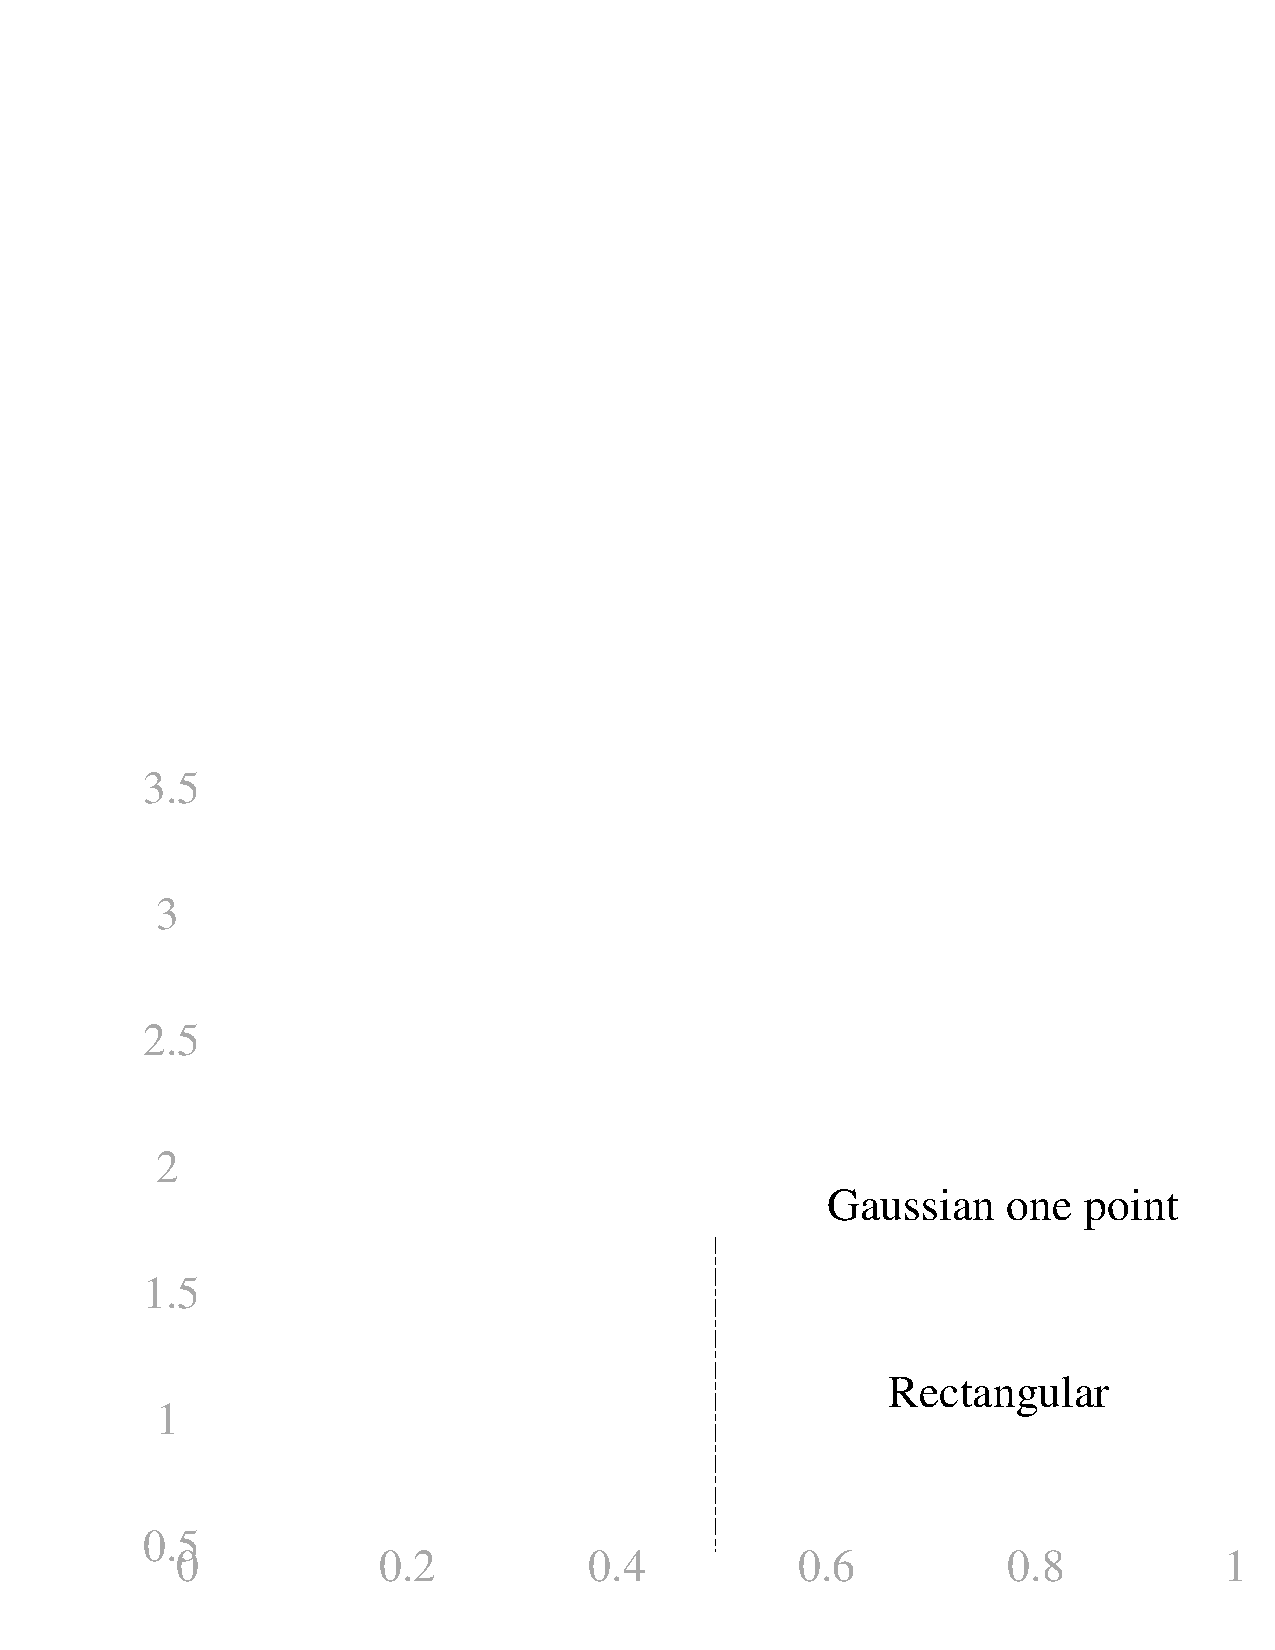
\includegraphics[width=6.53cm]{figs/gauss1.pdf}
%  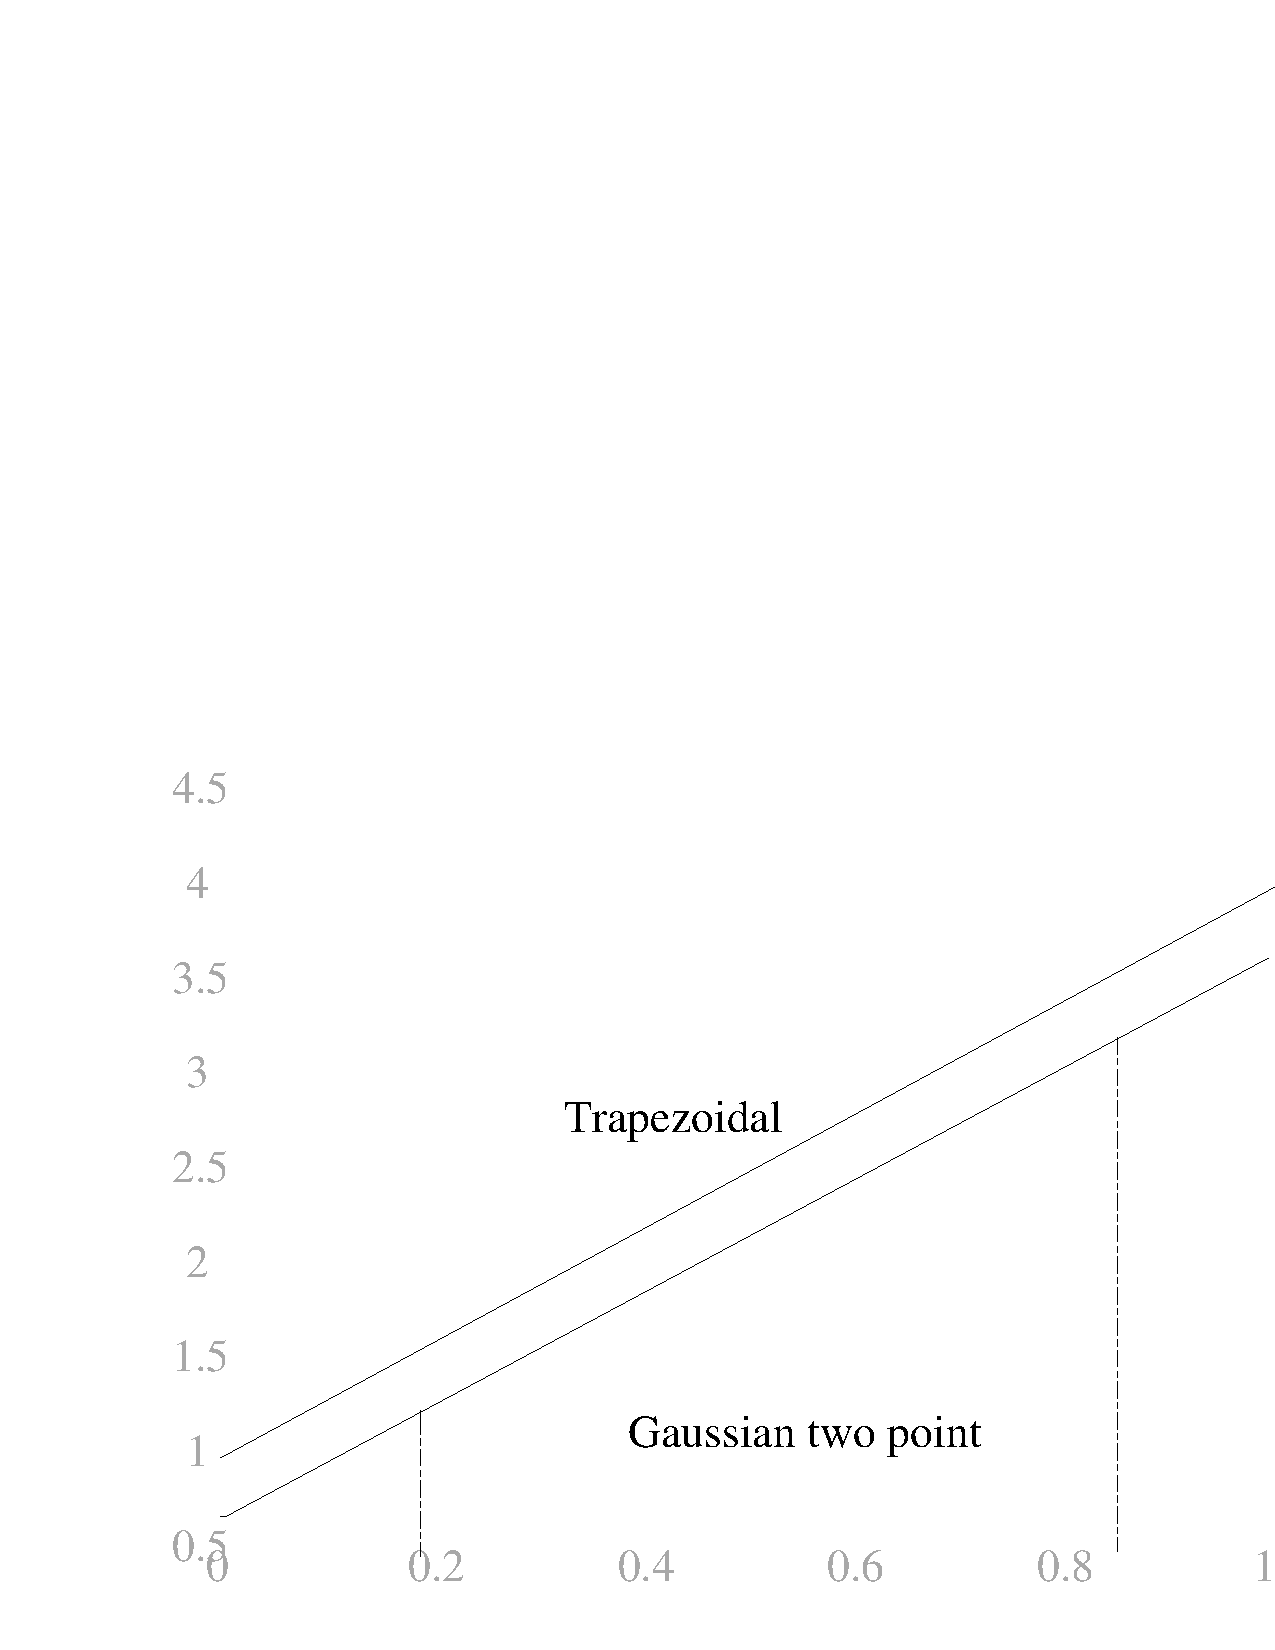
\includegraphics[width=6.53cm]{figs/gauss2.pdf}
%  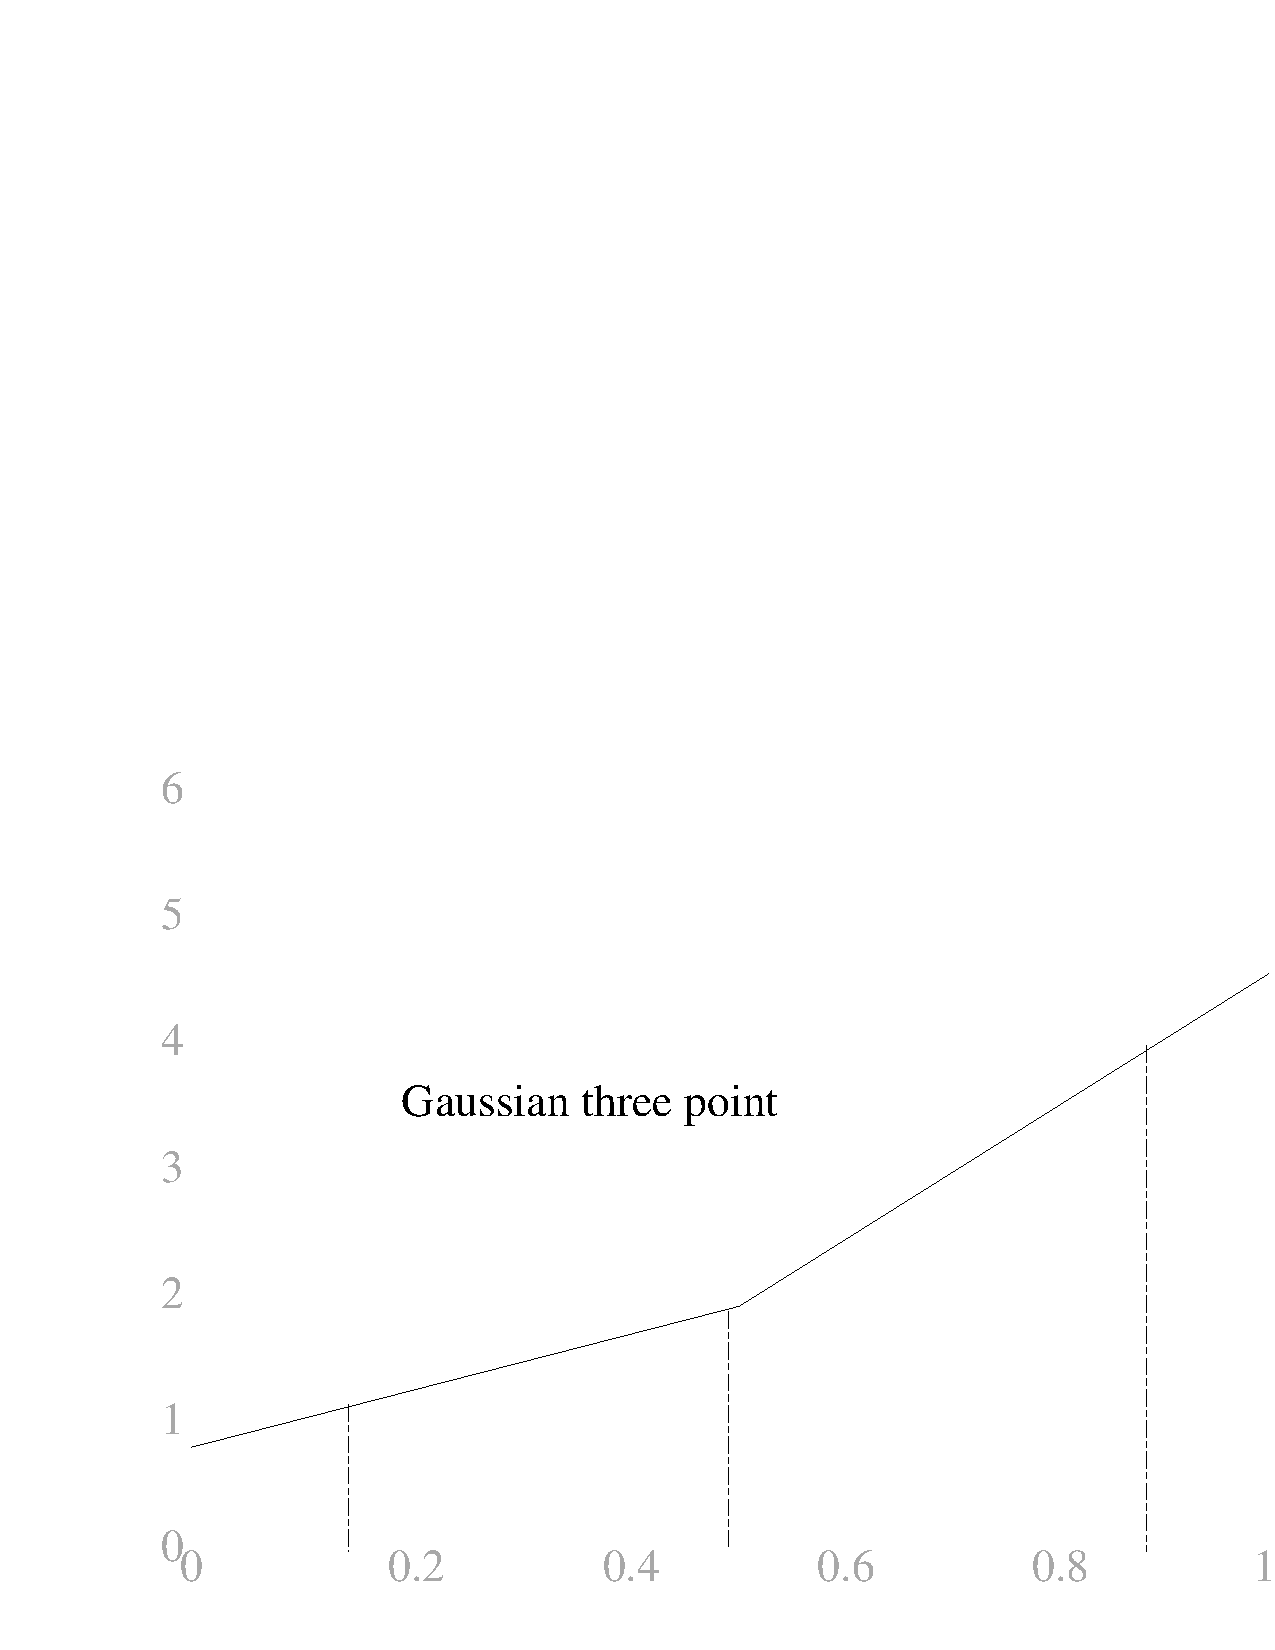
\includegraphics[width=6.53cm]{figs/gauss.pdf}
\caption{Numerical integration methods for general use and the corresponding Gaussian
    methods for use when there is no feedback. 1 - Rectangular - Gaussian one point; 
    2 - Trapezoidal - Gaussian two point; 3 - Gaussian three point}
\end{figure}
     
The three points of the Gaussian numerical integration are situated symmetrical around x =
0, in order to integrate the interval [-0.5,0.5]. Therefore, one of the three function
evaluation points will be at the center, x=0. The other two points will be located at either
side of the Y-axis at distance $\gamma$ (so x=-$\gamma$ and x=$\gamma$). Now the interval [-0.5 ,0.5] is divided
in three parts, around these three points. The lengths of these sub-intervals determine the
weights which must be imposed on the Y-values corresponding to these three x-values and
considered representative for their sub-interval. Because of the symmetry again, the weights
belonging to -$\gamma$ and $\gamma$ are equal. When these weights are considered 1, the weight of the
central sub-interval is equal to $\omega$.

The values of the relative distance $\gamma$ and of the weight $\omega$ can be derived from the
requirement that both the second and the fourth order terms of the polynomial will be
exactly integrated (Goudriaan, 1986):

\begin{align*}
  & Numerical \ result  & Analytical \ result\\
  2^{nd} order \qquad&  
    \frac{(-\gamma)^{2} + 0 \cdot \omega  + \gamma^{2}}{1+\omega +1} &= 
    \int_{-\frac{1}{2}}^{-\frac{1}{2}} x^2 dx &= \frac{1}{12}   \\
  4^{th} order \qquad&  
    \frac{(-\gamma)^{4} + 0 \cdot \omega +\gamma^{4} }{1 +\omega +1} &=
    \int_{-\frac{1}{2}}^{-\frac{1}{2}} x^4 dx &= \frac{1}{80}   \\
\end{align*}



\begin{align*}
 2^{nd} order & & 4^{th} order\\
 \frac{(-\gamma)^{2} + \gamma^{2}}{1 + \omega + 1} &= {\frac{1}{12}} &
 \frac{(-\gamma)^{4} + \gamma^{4}}{1 + \omega + 1} &= \frac{1}{80} \nonumber  \\
 \frac{2 \gamma^{2}}{2 + \omega} &= \frac{1}{12} & 
 \frac{2 \gamma^{4}}{2 + \omega} &= \frac{1}{80} \nonumber \\
 24 \gamma^{2} &= 2 + \omega  & 160 \gamma^{4} &= 2n+ \omega
\end{align*}

Substitution yields the following values for the relative distance and the weight:

\begin{align*}
\gamma =\sqrt{{\frac{24}{160}}} = \sqrt{0.15}  \\
\omega = 1.6
\end{align*}

\section*{Examples of the use of Gaussian Integration in the model}

Canopy assimilation is calculated as a weighted average of the assimilation at three
horizons within the canopy. The leaf area index of the selected horizons can be calculated
as:

\begin{align*}
 L &=~(0.5~+~p \sqrt{0.15} )LAI \qquad where \ p~=~-1,0,1 \Rightarrow  \\
L_{1} &= 0.1127017 \cdot LAI  \\
L_{2} &= 0.5 \cdot LAI   \\
L_{3} &= 0.8872983 \cdot LAI
\end{align*}

The weighted average of the assimilation over the three selected horizons is: 

\begin{align*}
A_{h} = \frac{LAI(A_{-1} ~+~1.6A _{0} ~+~A _{1} )}{3.6} \Rightarrow   \nonumber  \\
A_{h} = LAI(0.2778A_{-1} ~+~0.4444A_{0} ~+~0.2778A_{1} )
\end{align*}

Where:\\[5pt]]
\begin{tabularx}{\textwidth}{llXr}   
A$_{{\rm h}}$ &:& Hourly canopy assimilation & [g CO$_{{\rm 2}}$ m$^{{\rm -2}}$ h$^{{\rm -1}}$]\\
\end{tabularx}

To integrate the instantaneous canopy assimilation over the day, again the Gaussian
approach of numerical integration is applied. The three selected points refer to the period
from noon to sun set. Daily canopy assimilation is obtained as the weighted average of the
instantaneous assimilation rates at the selected time points:

\begin{align*}
t_{h} &= 12 ~+~ 0.5D(0.5~+~p \sqrt{0.15} ) \qquad where \ p =-1,0,1 \\
A_{d} &= \frac{D(A_{h,-1} + 1.6A_{h,o} + A_{h,1})}{3.6}
\end{align*}

Where:\\[5pt]
\begin{tabularx}{\textwidth}{lcXr}
D &:& Day length     &    [h]\\
th &:& Hour of day   &     [h]\\
A$_{{\rm d}}$ &:& Daily canopy assimilation    & 
    [g CO$_{{\rm 2}}$ m$^{{\rm -2}}$ d$^{{\rm -1}}$]\\
\end{tabularx}
\chapter{APPENDIX 2: AFGEN function} 

%\section*{AFGEN function}

{\bf AFGEN} stands for {\bf A}rbitrary {\bf F}unction {\bf GEN}erator. It is a fortran function 
which is used for
linear interpolation in a one-dimensional array with paired data. The uneven places in the
array represent the X-values, whereas the Y-values are represented by the even places of the
array. Such an array can be used to describe the dependency of variable Y of variable X in
case no mathematical description is available or is too cumbersome. A plotted example is
depicted in figure A2:

\begin{figure}[htbp]
 \centering
%     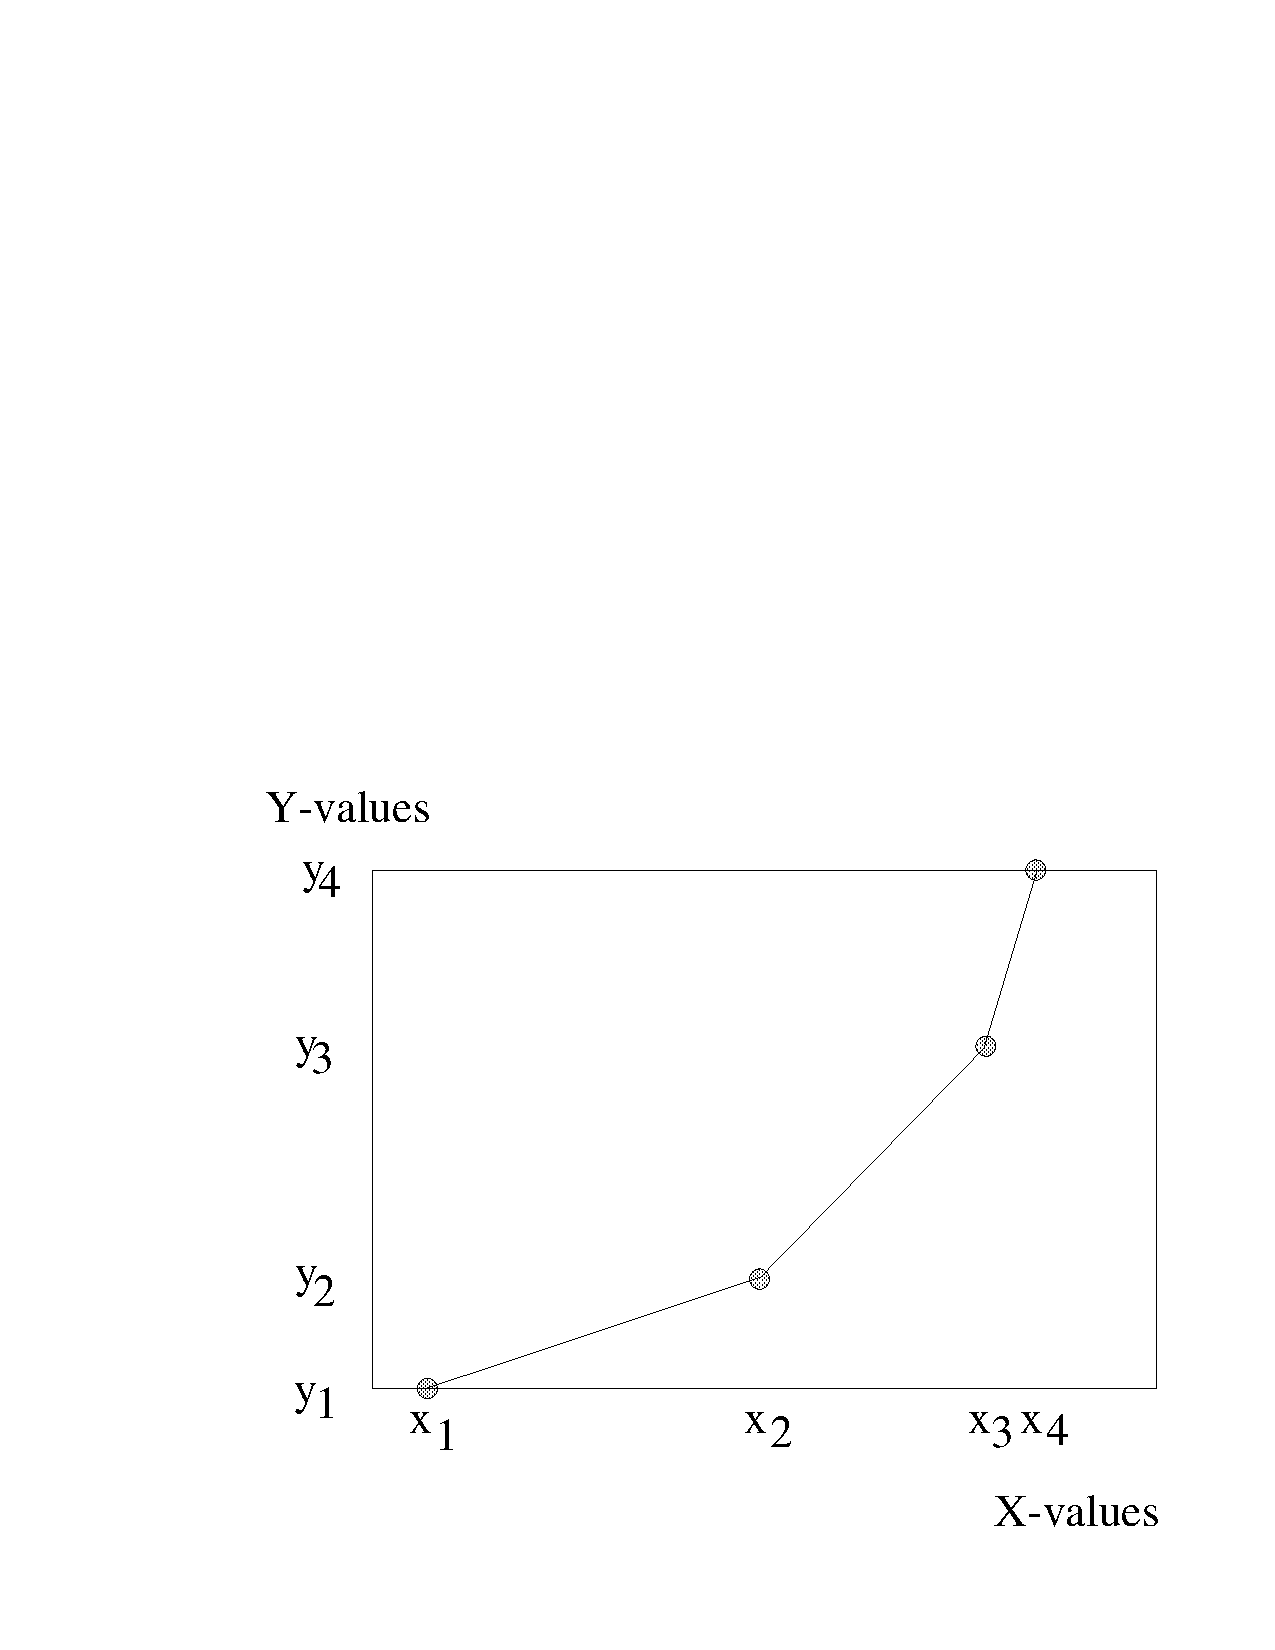
\includegraphics[0.8\textwidth]{figs/afgen.pdf}
 \caption{Linear interpolation}
 \label{fig:afgen}    
\end{figure}

The array belonging to this example has to be filled as:\\

\begin{center}
\begin{tabular}{lcccccccc}
Place & (1)& (2)& (3)& (4)& (5)& (6)& (7)& (8)\\
Value & X$_{{\rm 1}}$ & Y$_{{\rm 1}}$   & X$_{{\rm 2}}$& Y$_{{\rm 2}}$   & X$_{{\rm 3}}$ & Y$_{{\rm 3}}$   & X$_{{\rm 4}}$ & Y$_{{\rm 4}}$\\
\end{tabular}
\end{center}

The arguments of the AFGEN function in order of their place in the argument list are: name
of the table, number of pairs, X value to be interpolated. The X-values have to be arranged
from low to high values and are not allowed to be interchanged. Every X-value has to
precede its connected Y-value.

Three situations for interpolation can occur:

\begin{enumerate}
\item The argument {\it x} at which interpolation should take place is less or equal to the first
    X-value in the array. The Y-value is set to the first Y-value in the array.
\item The argument {\it x\/} value at which interpolation should take place is between the first
    and the last X-value in the array. The Y-value can now be found via linear
    interpolation. First the X values left and right from the argument {\it x\/} have to be
    detected, then the Y-value can be calculated:\\
    \begin{equation*}
    y~=~ Y _{n-1} ~+~ (\, x\, -\, X _{n-1} \, )\,{\frac{ Y _{n} \, -\, Y _{n-1} }{X _{n} \, -\, X _{n-1} }}
    \end{equation*}
\item The argument {\it x\/} at which interpolation should take place is equal to or larger then the
    last X-value in the array. The Y-value is set to the last Y-value in the array.
\end{enumerate}
\chapter{APPENDIX 3: Variables in WOFOST}

\section*{Crop specific variables}

\footnotesize
%\begin{longtable}[c]{lcll}
\begin{longtable}[c]{
       p{0.1\linewidth}p{0.1\linewidth}p{0.6\linewidth}p{0.2\linewidth}
       }
    
\hline \hline
\textbf{Acronym} & \textbf{Symbol} & \textbf{Description} & \textbf{Units}\\
\hline
\multicolumn{4}{l}{\textit{Initial values}}\\
LAIEM & & leaf area index at emergence   &    ha ha$^{{\rm -1}}$\\
TDWI & W & initial total dry weight of the crop  &     kg ha$^{{\rm -1}}$ \\
RGRLAI & RL & maximum relative increase in leaf area index  &     ha ha$^{{\rm -1}}$ d$^{{\rm -1}}$\\

\multicolumn{4}{l}{\textit{emergence}}\\
TBASEM & T$_{{\rm b}}$ & lower threshold temperature below which phenological 
  development stops &      \degrees C\\
TSUMEM & R & threshold temperature sum from sowing to emergence  &     \degrees C\\
TEFFMX & R & maximum effective temperature for emergence  &     \degrees C\\

\multicolumn{4}{l}{\textit{Phenology}}\\
DLC &  D$_{{\rm c}}$ & critical day length for development (lower threshold)   &    h\\
DLO & D$_{{\rm o}}$ & optimum day length for development    7   h\\
IDSL & - & indicates whether pre-anthesis development depends on temperature
  (0) temperature, (1) daylength, (2) temperature and daylength\\
DTSMTB & DT$_{{\rm s}}$ & daily increase in temperature sum as a function
  of temperature (AFGEN table)   &    \degrees C\\
TSUM1 & $\Sigma$T$_{{\rm i}}$ & threshold temperature sum from emergence to anthesis   &    \degrees C\\
TSUM2 & $\Sigma$T$_{{\rm i}}$ & threshold temperature sum from anthesis to maturity    &   \degrees C\\
DVSEND & - & development stage at harvest\\

\multicolumn{4}{l}{\textit{Green Area}}\\
SLATB & S$_{{\rm la}}$ & specific leaf area as a function of 
    development stage (AFGEN table)  &      ha kg$^{{\rm -1}}$\\
SPA & SS$_{{\rm so}}$ & specific pod area  &      ha kg$^{{\rm -1}}$\\
SPAN & - & life span of leaves growing at an average temperature of 35 \degrees C &  d\\
SSA & SS$_{{\rm st}}$ & specific stem area  &      ha kg$^{{\rm -1}}$\\

\multicolumn{4}{l}{\textit{Assimilation}}\\
AMAXTB & A$_{{\rm m}}$& maximum CO2 assimilation rate as a function of
    development stage of the crop (AFGEN table)   &    kg ha$^{{\rm -1}}$ h$^{{\rm -1}}$\\
EFF & $\epsilon$ & initial light use efficiency of CO2 assimilation of single leaves   &   
    kg ha$^{{\rm -1}}$ h$^{{\rm -1}}$ J$^{{\rm -1}}$ m$^{{\rm 2}}$s\\
KDIF & $\kappa$$_{{\rm df}}$ &extinction coefficient for diffuse visible light   &    -\\
TMNFTB & -& correction factor of daily gross CO2 assimilation rate as a
    function of T$_{{\rm low}}$ (AFGEN table)  &     \degrees C\\
TMPFTB & - &correction factor of maximum leaf CO2 assimila\-tion rate as a
    function of sub-optimum average day temperatu\-res, T$_{{\rm day}}$ (AFGEN table)  & 
    \degrees C\\

\multicolumn{4}{l}{\textit{Conversion of assimilates into biomass}}\\
CVL & C$_{{\rm e,lv}}$ & efficiency conversion of assimilates into leaf dry 
    matter   &    kg kg$^{{\rm -1}}$\\
CVO & C$_{{\rm e,so}}$ & efficiency conversion of assimilates into storage organ 
    dry matter   &    kg kg$^{{\rm -1}}$\\
CVR &  C$_{{\rm e,rt}}$ & efficiency conversion of assimilates into root dry 
    matter    &   kg kg$^{{\rm -1}}$\\
CVS &  C$_{{\rm e,st}}$ & efficiency conversion of assimilates into stem dry 
    matter  &     kg kg$^{{\rm -1}}$\\

\multicolumn{4}{l}{\textit{Maintenance respiration}}\\
Q10 & Q$_{{\rm 10}}$ & increase of the respiration rate per 10\degrees C
temperature increase    &   kg ha$^{{\rm -1}}$ d$^{{\rm -1}}$\\
FSETB & - & reduction factor for the maintenance respiration as a function \\
  of DVS (AFGEN table)       -\\
RML & c$_{{\rm m,lv}}$ & maintenance respiration rate coefficient of leaves       d$^{{\rm -1}}$\\
RMO & c$_{{\rm m,so}}$ & maintenance respiration rate coefficient of storage organs       d$^{{\rm -1}}$\\
RMS & c$_{{\rm m,rt}}$ & maintenance respiration rate coefficient of stems       d$^{{\rm -1}}$ \\
RMR & c$_{{\rm m,rt}}$ & maintenance respiration rate coefficient of roots       d$^{{\rm -1}}$ \\

\multicolumn{4}{l}{\textit{Maintenance respiration}}\\
FLTB & pc$_{{\rm lv}}$ & fraction of above-ground dry-matter increase partitioned to leaves
  as a function of development stage (AFGEN table)    &   -\\
FOTB & pc$_{{\rm so}}$ & fraction of above-ground dry-matter increase partitioned to storage
  organs as a function of development stage (AFGEN table)    &   -\\
FRTB & pc$_{{\rm rt}}$ & fraction of total dry-matter increase partitioned to roots
  as a function of development stage (AFGEN table)   &    -\\
FSTB & pc$_{{\rm st}}$ & fraction of above-ground dry-matter increase partitioned to stems
  as a function of development stage (AFGEN table)   &    -\\

\multicolumn{4}{l}{\textit{Death rate}}\\
PERDL & \dag $_{{\rm max,lv}}$ & maximum relative death rate of leaves due to water stress &
   d$^{{\rm -1}}$\\
RDRRTB & \dag $_{{\rm rt}}$ & relative death rate of roots as a function of DVS (AFGEN table) &
   kg kg$^{{\rm -1}}$ d$^{{\rm -1}}$\\
RDRSTB & \dag $_{{\rm st}}$ & relative death rate of stems as a function of DVS (AFGEN table) &\
   kg kg$^{{\rm -1}}$ d$^{{\rm -1}}$\\
TBASE & T$_{{\rm b,age}}$ & lower threshold temperature for physiological ageing of leaves  &
    \degrees C \\

\multicolumn{4}{l}{\textit{Water use}}\\
CFET & - & correction factor for evapotranspiration    &   -\\
DEPNR & No$_{{\rm cg}}$ & crop group number   &    -\\
IAIRDU & - & indicates presence (1) or absence (0) of airducts in the plant &   -\\

\multicolumn{4}{l}{\textit{Rooting}}\\
RDI & RD$_{{\rm I}}$ & initial rooting depth   &    cm\\
RDMCR & RD$_{{\rm crop}}$ & crop-dependent maximum rooting depth    &   cm\\
RDMSOL & RD$_{{\rm soil}}$ & soil-dependent maximum rooting depth   &    cm\\
RRI & RR$_{{\rm max}}$ & maximum daily increase of rooting depth   &    cm d$^{{\rm -1}}$\\

\hline \hline
                      
\end{longtable}
\normalfont
 
\section*{Soil specific variables}

\small
\begin{longtable}[c]{llll}
\hline \hline
\textbf{Acronym} & \textbf{Symbol} & \textbf{Description} & \textbf{Units}\\
\hline

\multicolumn{4}{l}{\textit{Soil water retention}}\\   
SMW & $\theta$$_{{\rm wp}}$ & soil moisture content at wilting point    &
   cm$^{{\rm 3}}$ cm$^{{\rm -3}}$\\
SMFCF & $\theta$$_{{\rm fc}}$ & soil moisture content at field capacity   &
   cm$^{{\rm 3}}$ cm$^{{\rm -3}}$\\
SM0 & $\theta$$_{{\rm max}}$ & soil porosity   &    cm$^{{\rm 3}}$ cm$^{{\rm -3}}$\\
WAV & W$_{{\rm av}}$ & initial available soil water amount in excess of 
   $\theta$$_{{\rm wp}}$   &    cm\\
NOTINF & F$_{{\rm I}}$ & maximum fraction of rain not infiltrating into the 
   soil   &    -\\
CRAIRC & $\theta$$_{{\rm c}}$ & critical soil air content    &
   cm$^{{\rm 3}}$ cm$^{{\rm -3}}$\\
CONTAB & K(pF) & $^{{\rm 10}}$log hydraulic conductivity as a function of the pF 
(AFGEN table)   &    log(cm)\\

\multicolumn{4}{l}{\textit{Percolation}}\\   
K0 & K & hydraulic conductivity   &    cm d$^{{\rm -1}}$\\
SOPE & - & maximum percolation rate rote zone   &    cm d$^{{\rm -1}}$\\
KSUB & - & maximum percolation rate subsoil   &    cm d$^{{\rm -1}}$\\
SSMAX & SS$_{{\rm max}}$ & maximum surface storage capacity   &    cm\\
DD & DD & drainage depth   &    cm\\
ZTI & - & initial depth of the groundwater table   &    cm\\

\multicolumn{4}{l}{\textit{Soil workability}}\\   
SPADS & Sp$_{{\rm 1}}$ & first topsoil seepage parameter, deep seedbed       -\\
SPODS & Sp$_{{\rm 2}}$ & second topsoil seepage parameter, deep seedbed       -\\
SPASS & Sp$_{{\rm 1}}$ & first topsoil seepage parameter, shallow seedbed       -\\
SPOSS & Sp$_{{\rm 2}}$ & second topsoil seepage parameter, shallow seedbed       -\\
IDESOW & - & earliest sowing date       -\\
IDLSOW & - & latest sowing date       -\\

\hline \hline

\end{longtable}
\normalfont


\end{document}
